% !TEX encoding = UTF-8 Unicode
% !BIB TS-program = biber 
% !BIB program = biber    

% This file is MIT-Thesis.tex, a LaTeX template for formatting an MIT thesis with the mitthesis class.
%
% Version: 1.11, 2023/11/02
%
% Author: John H. Lienhard, copyright 2023. Reuse under the MIT license: https://ctan.org/license/mit 

% Documentation is here: https://ctan.org/pkg/mitthesis

%% Don't modify the \DocumentMetadata command unless you know what it does. 
%% If this command throws an "undefined" error, your latex system is out of date: try commenting this command out.
\DocumentMetadata{ 
	pdfstandard = a-2b,
	pdfversion  = 1.7,
	lang		= en-US,
%	debug		= {xmp-export}, % uncomment to output a separate xmpi file showing the metadata
}
%%%%%%%%%%%%%%%%%%%%%%%%%%%%%%%%%%%%%%%

\documentclass[twoside]{mitthesis} %,fontset=libertine, fontset=newtx-sans-text, fontset=heros-stix2, fontset=stix2
%
% option [twoside]		gives facing-page behavior for printing; omitting twoside will eliminate even-numbered blank pages.
% option [lineno]	 	provides line numbers, as for editing
% option [mydesign] 	loads packages for color, title and list formats, margins, or captions: edit mydesign.tex to change defaults.
% option [fontset] is a keyvalue which can be:
%					 	pdftex or unicode engines:  defaultfonts, libertine, lucida
%					 	pdftex only: 				fira-newtxsf, newtx, newtx-sans-text
%						unicode engines (luatex):	heros-stix2, stix2, termes, termes-stix2
%					 	if no key value is given, fonts default to CMR (pdftex) or LMR (unicode), i.e., "the LaTeX font".
%					 	You can edit the fontset files or you can write your own, myfonts.tex, and do [fontset=myfonts].
%						If you are using multiple languages, load the babel package in your fontset file, before the fonts.

\usepackage{amsmath}
\usepackage{graphicx}
\usepackage{mathtools}		% for obscure math commands
\usepackage{amssymb}		% for obscure math symbols
\usepackage{amsfonts} 		% for obscure math fonts
\usepackage{float}			% [H] float command
\usepackage{subcaption} 	% for subfigure captions
\usepackage{sidecap}		% for figure side captions
\usepackage{makecell}		% formatting cells within tabular with \thead and \makecell
\usepackage{multicol} 		% for tabular \multicolumn 
\usepackage{multirow} 		% for tabular - \multirow
% \usepackage{hyperref}		% urls
\PassOptionsToPackage{hyphens}{url}\usepackage{hyperref}	% urls that linebreak
\usepackage{import}			% import subfiles
\usepackage{longtable}		% tables extend multiple pages \begin{longtable}{}
\usepackage{ltablex}		% provides tabularx, page breaking capabilities
\usepackage{rotating}		% sideways and rotate package
\usepackage{bbm}  % for indicator function
\usepackage{soul}  % for underline

\usepackage{fancyhdr}		% Fancy headers
\usepackage{setspace}		% double or set spacing
\usepackage{wrapfig}		% wrap figures around text
\usepackage{booktabs}		% top, mid and bottom rule for tables
\usepackage{rotating}		% writing vertically using \begin{turn} ... \end{turn}
\usepackage{amssymb}		% random symbols like checkmarks
\usepackage{enumitem}		% modifications to enumerated list
\usepackage{siunitx}		% include SI units in math mode
\usepackage{adjustbox}		% rescale tables to fit page
\usepackage{changepage}   	% for the adjustwidth environment
\usepackage[hang,flushmargin,bottom]{footmisc} 	% foot notes go on the bottom and no indent
\usepackage{cleveref}		% multi-clever referencing
\usepackage{pdfpages}		% add external pdf module
\usepackage{enumitem}		% enumerate referenced items
\usepackage{amsmath,amssymb,amsfonts,amsthm}
% \usepackage{algorithmic}
\usepackage[linesnumbered,ruled,vlined,resetcount,algosection]{algorithm2e}
\usepackage{algpseudocode}

%% Algorithm keywords
\SetKwInput{KwInput}{Input}                % Set the Input
\SetKwInput{KwOutput}{Output}              % set the Output
\SetKw{Break}{break}

% Theorem setup
\newtheorem{theorem}{Theorem}[section]
\newtheorem{lemma}[theorem]{Lemma}

%%%%%%%%%  Graphics path (to figure files)  %%%%%%%%%%%%%%%%%%%%%%%%%%%%%%%%

%% Can set graphicspath to point to specific directories containing figures (the current directory is searched automatically)
%% For instance, to search a subdirectory of the current directory called "figures" and a parallel directory called "art", set:

% \graphicspath{ {figures/} {../art/} }% For details see: https://latexref.xyz/dev/latex2e.html#g_t_005cgraphicspath

\graphicspath{ {images/} }

%%%%%%%%%  Representative set-up for biblatex  %%%%%%%%%%%%%%%%%%%%%%%%%%%%%

\usepackage[backend=biber,style=ieee,maxbibnames=10,sorting=none]{biblatex}% style=ext-numeric-comp,articlein=false,giveninits=true
	\DefineBibliographyStrings{english}{url= \textsc{url} ,  }% replaces default "[Online]. Available" by "URL"


\addbibresource{main.bib}

\usepackage{mymacros}

%% to avoid split urls and stretched white space, you can set the bibliography ragged-right:
%\appto{\bibsetup}{\raggedright}

% biblatex is very powerful, and you can customize most aspects the reference list and citations to suit your needs.
% documentation is here: https://ctan.org/pkg/biblatex


%%%%%%%%%%  Option to use natbib   %%%%%%%%%%%%%%%%%%%%%%%%%%%%%%%%%%%%%%%%%

%\RequirePackage[numbers,sort&compress]{natbib}
 
%%% add bibliography to table of contents
%\apptocmd{\bibliography}{\addcontentsline{toc}{chapter}{\protect\textbf{\bibname}}}{}{}

%%% You can use this to rename the bibliography section
%\renewcommand{\bibname}{References}

%%% Can adjust space between bibliography items (change 4pt to something else; don't drop last two lengths, they are stretchable "glue")
%\setlength\bibsep{4pt plus 1pt minus 1pt}


%%%%%%%%%%  Table related packages  %%%%%%%%%%%%%%%%%%%%%%%%%%%%%%%%%%%%%%%%

\usepackage{booktabs}% better quality tables, https://ctan.org/pkg/booktabs
\usepackage{array}%    additional options for table columns, https://ctan.org/pkg/array

%\usepackage{tabularx}%   https://ctan.org/pkg/tabularx

%\usepackage{dcolumn}%    alignment on decimal place, https://ctan.org/pkg/dcolumn
%\newcolumntype{d}[1]{D{.}{.}{#1}}


%%%%%%%%%%  Option for "double spacing" %%%%%%%%%%%%%%%%%%%%%%%%%%%%%%%%%%%%

%% Back in the typewriter era, double spaced lines were convenient for editing with a pencil. 
%% In typography, the separation between lines is called "leading", and it is usually set in 
%% proportion to the font size (i.e., when the font is loaded).  If you really feel the need 
%% to change the line separation, the most attractive results will be obtained by changing the
%% leading in proportion to the the current font size, rather than just doubling the space.

%% The setspace package provides a tool for changing line separation. Use these two commands here:
%
% \usepackage{setspace}%  documentation at https://ctan.org/pkg/setspace
% \setstretch{1.1}% you can choose some other value for the stretch of space between lines
%
%% Use one or more of the these commands AFTER the frontmatter
%
% \onehalfspacing
% \doublespacing
% \singlespacing  % will turn these effects off (you can use these anywhere in the document)

%% The best result may be to stay with leading selected by the typographer who set up the font.


%%%%%%%%%%%  Metadata  %%%%%%%%%%%%%%%%%%%%%%%%%%%%%%%%%%%%%%%%%%%%%%%%%%%%%%%

% Most of the document metadata is created automatically. 
% The following items should be adjusted to match your work. <================= !!!!!!!!!!

\hypersetup{%  % TODO
	pdfsubject={Template for writing MIT theses with the mitthesis class},
	% Change this to briefly state topic of your thesis 
% 
	pdfkeywords={Massachusetts Institute of Technology, MIT},
	% Add keywords that will help search engines and libraries to find your work.
	% Includes the name[s] of the author[s] 
	% (If you have used \DocumentMetadata, at line 15, you can just put "\CopyrightAuthor," for the names.)
%
	pdfurl={},
	% If you have a url for the thesis, put it here. Otherwise delete this.
	% (MIT Libraries will put your thesis in DSPACE with a persistent url after you submit it.)
%	
	pdfcontactemail={},
	% You can put a [permanent] email address into the metadata, if you like.
	% Otherwise delete this.
%
	pdfauthortitle={},
	% If you have a title, you can include it here.
}

%%%%%%%%%%%%%%  End preamble %%%%%%%%%%%%%%%%%%%%%%%%%%%%%%%%%%%%%%%%%%%%%%%%%%%%%%%%%%%%%%%%%%%%%
%%%%%%%%%%%%%%%%%%%%%%%%%%%%%%%%%%%%%%%%%%%%%%%%%%%%%%%%%%%%%%%%%%%%%%%%%%%%%%%%%%%%%%%%%%%%%%%%%%

\begin{document}

%%% edit the following commands to match your thesis %%%%%%%%%%

\title{Safety in an uncertain world: model-based verification-guided design for safety-critcial autonomous systems}

% \Author{Author full name}{Author department}[Author's first PREVIOUS degree][Author's second PREVIOUS degree][...
% Note that third, fourth, fifth, and sixth arguments are optional [] and may be omitted

% note on names: most of the following names are made up; Silas Holman was a physics professor at MIT in the 19th century.

\Author{Charles Burke Dawson}{Department of Aeronautics and Astronautics}[B.S. Engineering, Harvey Mudd College, 2019][M.S. Aeronautics and Astronautics, MIT, 2021]

% Use once for each degree fulfilled by thesis
% For two degrees from one department, leave the department argument blank for the second degree {}.
% \Degree{Bachelor of Science in Physics}{Department of Physics}
% \Degree{Master of Science in Physics}{}
\Degree{Doctor of Philosophy}{Department of Aeronautics and Astronautics}

% If there is more than one supervisor, use the \Supervisor command for each.
\Supervisor{Chuchu Fan}{Associate Professor of Aeronautics and Astronautics}
% \Supervisor{Russ Tedrake}{Professor of Electrical Engineering and Computer Science}
% \Supervisor{Serta\c c Karaman}{Professor of Aeronautics and Astronautics}

% Professor who formally accepts theses for your department (e.g., the Graduate Officer, Professor Sméagol,...)
% If more than one department, use more than once
% **If you need to reduce vertical space, put the acceptor title in the second argument and leave the third blank {}.**
\Acceptor{Jonathan P. How}{Professor of Aeronautics and Astronautics}{Chair, Graduate Program Committee, Department of Aeronautics and Astronautics}

% Usage: \DegreeDate{Month}{year}
% Valid degree months are September, February, or June
\DegreeDate{May}{2024}

% Date that final thesis is submitted to department
\ThesisDate{May 16, 2024}  % TODO

%%%%%%  Choose whether to have a CREATIVE COMMONS License  %%%%%%%%%%%%%%%%%%%%%%%%%%%%%%%%%%%%%%
%
% If you are using a cc license, put details of your cc license here. 
% Omit this command if you are not using a cc license.
%
\CClicense{CC BY-NC-ND 4.0}{https://creativecommons.org/licenses/by-nc-nd/4.0/}
%

%%%%%%%  Solutions for overflowing titlepage  %%%%%%%%%%%%%%%%%%%%%%%%%%%%%%%%%%%%%%%%%%%%%%%%%%%

% If your title page is overflowing (from too many names, degrees, etc.):
%
% (a) you can reduce the 12pt and 18pt skips between various blocks to 6pt with this command:
%
% \Tighten
%
% (b)  you can scale down the Signature block at the bottom with this command:
%
% \SignatureBlockSize{\small}  %or this one \SignatureBlockSize{\footnotesize}
%
% (c) you can put the acceptor name and title onto two lines, rather than three like this:
%
% \Acceptor{Tertius Castor}{Professor and Graduate Officer, Department of Research}{}
% \Acceptor{Quarta Castor}{Professor and Graduate Officer, Department of Mechanical Engineering}{}
%
% (d) you can change the font size of the the author name[s] with
%
%	\AuthorNameSize{\normalsize}
%
% (e) and you can omit any previous degrees from the title page, instead mentioning them in the Biosketch

% Also, if you prefer to keep the text toward the top of the page with most white space at the bottom, you
% can you this command to squash all of the vertical glue (stretchy space) with this command:
%
% \Squash 
%
% This command is useful when the text has not already reach the bottom of the page, since the glue gets squashed automatically
% when the page is too full.

%%%%%%%%%%%%%%%%%%%%%%%%%%%%%%%%%%%%%%%%%%%%%%%%%%%%%%%%%%%%%%%%%%%%%%%%%%%%%%%%%%%%%%%%%%%%%%%%%

%%% Make titlepage
\maketitle

%%%%%%%%% Contents that you need to write follows %%%%%%%%%%%%%%%%%%%%%%%%%%%%%%%%%%%%%%%%%%%%%%%%

% \includeonly{acknowledgments,biography,chapter1,chapter2,...,appendixa,...} 
%   for usage, see https://latexref.xyz/_005cinclude-_0026-_005cincludeonly.html

%%% Frontmatter (write this material in the mentioned files)  %%%%%%%%%%%%%%%%%%%%%%%%%%%%%%%%%%%%

% The abstract environment creates all the required headings and footers. 
% You only need to the text of the abstract in the file abstract.tex
\begin{abstract}
	% From mitthesis package
% Version: 1.01, 2023/06/19
% Documentation: https://ctan.org/pkg/mitthesis
%
% The abstract environment creates all the required headers and footnote. 
% You only need to add the text of the abstract itself.
%
% Approximately 500 words or less; try not to use formulas or special characters
% If you don't want an initial indentation, do \noindent at the start of the abstract

Before robots can be deployed in safety-critical environments, we must be able to verify they they will perform safely, ideally without the risk and expense of real-world testing. A wide variety of formal methods and simulation-driven techniques have been developed to solve this verification problem, but they typically rely on difficult-to-construct mathematical models or else use sample-inefficient black-box optimization methods. Moreover, existing verification methods provide little guidance on how to optimize the system's design to be more robust to the failures they uncover.
%
In this thesis, we develop a suite of methods that accelerate verification and design automation of robots and other autonomous systems by using program analysis tools such as automatic differentiation and probabilistic programming to automatically construct mathematical models of the system under test. In particular, we make the following contributions. First, we use automatic differentiation to develop a flexible, general-purpose framework for end-to-end design automation and statistical safety verification for autonomous systems. Second, we improve the sample efficiency of end-to-end optimization using adversarial optimization to falsify differentiable formal specifications of desired robot behavior. Third, we provide a novel reformulation of the design and verification problem using Bayesian inference to predict a more diverse set of challenging adversarial failure modes. Finally, we present a data-driven method for root-cause failure diagnosis, allowing system designers to infer what factors may have contributed to failure based on noisy data from real-world deployments.
%
We apply the methods developed in this thesis to a range of challenging problems in robotics and cyberphysical system. We demonstrate the use of our design and verification framework to optimize spacecraft trajectory and control systems, multi-agent formation and communication strategies, vision-in-the-loop controllers for autonomous vehicles, and robust generation dispatch for electrical power systems, and we apply our failure diagnosis tool on real-world data from scheduling failures in a nationwide air transportation network.% use \input rather than \include because we're inside an environment
\end{abstract}

%% acknowledgments.tex

% From mitthesis package
% Version: 1.01, 2023/10/16
% Documentation: https://ctan.org/pkg/mitthesis


\chapter*{Acknowledgments}
\addcontentsline{toc}{chapter}{Acknowledgments}

I am lucky to have had an array of supporters throughout my PhD, each of whom deserves thanks for their role in this adventure. First, to my advisor, Professor Chuchu Fan: thank you for bringing me into your lab nearly four years ago, coaching me through the ups and downs of academic life, and giving me space to explore new research interests. Our weekly discussions provided a great source of perspective, support, and (when needed) challenge, and I am a better researcher for having had the privilege of working with you. In addition, thank you to my undergraduate advisors, Professors Kash Gokli and Philip Cha, for starting me on my academic journey with just the right combination of support and independence.

Next, to my thesis committee and research collaborators. Professors Russ Tedrake and Serta\c c Karaman, thank you for your helpful discussions and feedback as I progressed from blurry vision to completed PhD. To Professors Sicun Gao and Max Li, thank you for the opportunity to work together at the start and end of my PhD journey, respectively. To Chelsea, Yang, Austin, and Falk: I'm grateful that we had the chance to collaborate and learn from each other's perspectives. To Chafik, Rachel, Jake, Fayez, Gee, Tyler, Jordyn, Britany, and the rest of the team at Marble, thanks for having me along for the ride!

I am also grateful for the countless conversations, both personal and research-related, with my labmates over the years: Kunal, Jake, Kwesi, Yue, Songyuan, Ji, Anjali, Oswin, Mingxin, Yongchao, Ruixiao, Yilun, Cheng, Allen, Laura, Chenning, Rujul, Sydney, Zengyi, and Kathleen. In addition, I am lucky to have had the opportunity to mentor a number of fantastic undergraduate researchers during my PhD: Dylan, Bethany, Mukun, Suchitha, Jenny, and Van. Hopefully you learned as much from working with me as I did from working with you. I know that you will all accomplish great things in the coming years.

Beyond MIT, thank you to the friends who have kept me sane over the last 5 years. To my friends from Harvey Mudd, Camille, Maggie, Alex, Sara, Katie, and Brenden: thank you for countless catch-up calls and apple-picking adventures. To my friends in Boston, Riley, Matt, Fran, James, Annie, Avi, and Leah: thank you for good times and board games, climbing, and canoeing. To Evan: thank you for your level-headed advice and good-natured humor.

Most importantly, thank you to my family. To Mom and Dad: I don't think a paragraph or even a whole thesis would be enough to say thank you for your boundless love and support. You've been there for me every step of the way, and I'm so grateful for you. To Grandma and Grandpa: you two are the best role models I could have asked for, both as educators and as loving, supportive human beings. To my brother, Henry: it has been such a privilege to grow up with you --- I'm a better person for having you as a brother, and I can't wait to see what you do next on your own journey.

Finally, to the love of my life, Lydia: words are not enough, but I can try. Thank you for being there with me through the ups and downs of both life and my PhD. Your compassion, intelligence, and sheer zest for life inspire me every day, and there's no place I would rather be than with you. You are the best, I love you, and I'm looking forward to discovering what the next chapter holds.
% .tex extension is presumed by \include 

%%% Table of contents and lists of stuff (delete lists you don't need, e.g., if no tables) %%%%%%%%

\tableofcontents
\listoffigures
\listoftables


%%% Chapters of thesis  %%%%%%%%%%%%%%%%%%%%%%%%%%%%%%%%%%%%%%%%%%%%%%%%%%%%%%%%%%%%%%%%%%%%%%%%%%%

%% If you want to use "double spacing", you should start here...
\onehalfspacing

%% TODO: update subsections to sections (so top level is chapter, then section, then subsection)

\chapter{Introduction}\label{section:introduction}

Before robots can be deployed in safety-critical environments, we must be able to verify that they will perform safely. Unfortunately, as robots and other cyberphysical systems become more complex, they become harder for human engineers to test, verify, and debug. For example, autonomous vehicle (AV) operators rely on a combination of low-fidelity but inexpensive testing on massively-parallel simulation and more expensive but higher fidelity testing on physical hardware. Despite large amounts of time, money, and engineering effort invested in these systems, AVs have struggled to reach the required high degree of reliability and still encounter unforeseen, life-threatening corner cases in the wild. The challenge of testing and debugging safety-critical cyberphysical systems is not particular to AVs; for instance, as the electric power grid is increasingly automated to deal with variable sources of renewable energy, or as airspace is increasingly occupied by unmanned aerial vehicles, it will be crucial to ensure that the associated prediction and control algorithms are thoroughly tested before deployment.

In cases where real-world testing is too risky or expensive, engineers must instead rely on mathematical modeling and simulation to verify that a robot will perform as intended. Unfortunately, there are issues with each of these approaches. Although mathematical models are amenable to formal proofs, robots are often too complex to reduce to a set of equations. On the other hand, although simulators can handle the full complexity of a robotic system, they are often treated as black-boxes, providing an incomplete view of a robot's performance. In order to safely deploy complex robots in the real world, we require new tools that blend the rigor of mathematical modeling with the scalability and generality of simulation.

This thesis aims to close the gap between formal methods based on mathematical models~\cite{beltaFormalMethodsControl2019,kress-gazitSynthesisRobotsGuarantees2018} and simulation-based verification techniques~\cite{zhouRoCUSRobotController2021,corsoSurveyAlgorithmsBlackBox2021,okellyScalableEndtoEndAutonomous2018} to develop tools to help engineers more easily design and verify complex robotic systems. Our key insight is that simulators, as computer programs, are not black boxes but instead contain rich mathematical structure. If we can exploit this structure using program analysis tools (e.g. automatic differentiation, tracing, etc.), we can improve the efficiency, flexibility, and rigor of simulation-based approaches.

\section{Thesis contributions}

Using this insight, we develop tools to support the design and analysis process for robots and other safety-critical cyberphysical systems in four ways:
\begin{enumerate}
    \item \textit{Design optimization:} automatically search for design parameters that achieve good performance.
    \item \textit{Safety verification:} characterize the robustness of a design and predict corner cases where it is likely to fail (by either violating a constraint or incurring a high cost).
    \item \textit{Verification-guided design:} closing the feedback loop between verification and design; e.g., by using predicted corner cases to guide future design iterations.
    \item \textit{Anomaly diagnosis:} explain the root causes of unexpected behavior observed in deployed systems.
\end{enumerate}
%
The goal of this thesis is to provide tools that will support engineers in developing increasingly complex robotic systems, enabling a more efficient design process and providing the ability to verify the safety of a design \textit{before} deployment. The following sections provide a summary of the contributions of this thesis in each of these areas before concluding with an outline of the rest of this document.

\subsection{End-to-end design optimization and robustness certification}

Practical robotic and cyberphysical systems often have diverse subsystems that do not lend themselves to easy mathematical abstraction and formal analysis. For example, it would be difficult to develop a formal mathematical model for the interactions between planning, perception, and control subsystems. Further complicating matters, these systems must operate reliably in uncertainty environments. This combination of complexity and uncertainty makes it difficult to design and verify these systems, especially when some subsystems contain machine learning models with thousands of tunable parameters and difficult-to-interpret behaviors.

To address these challenges, we develop an automated tool that enables efficient optimization and statistical robustness certification of robot designs. Our framework uses differentiable programming for end-to-end optimization of robotic systems, allowing users to flexibly model interactions between subsystems and the effect of environmental uncertainty. In addition, we develop a novel statistical framework for certifying the worst-case performance and sensitivity of optimized designs. We apply these tools to optimize the design of two robotic systems in hardware, using statistical certification to verify robustness before transferring the optimized designs to hardware without fine-tuning.

\subsection{Improving design robustness using counterexamples for formal specifications}

Although end-to-end design optimization provides a flexible means of optimizing robot behaviors, prior approaches to design optimization rely on domain randomization over a large number of environments to encourage robustness~\cite{tobinDomainRandomizationTransferring2017,dawsonCertifiableRobotDesign2022}. This approach is not only computationally expensive, but it also risks missing important corner cases if the set of training examples is too small.

In this thesis, we improve the sample efficiency of end-to-end design optimization techniques by incorporating adversarial optimization methods to search for counterexamples to formal specifications of robot behavior. We use differentiable temporal logic to specify high-level safety and performance requirements, then use adversarial optimization to search for the worst-case counterexamples falsifying these requirements. We show that feeding these adversarial counterexamples back into the design optimization process yields more robust designs while requiring far fewer samples than standard domain randomization techniques.

\subsection{Predicting and repairing diverse failure modes}

The end-to-end design and verification methods discussed so far have the advantage of using gradients from automatic differentiation to speed the search for high-performing designs and challenging failure modes, but there are a number of drawbacks to these gradient-based methods. In particular, because gradient-based methods quickly converge to local optima, they struggle to find a set of qualitatively different failure modes. Instead, nearby failure modes collapse into a single ``most severe'' mode. Moreover, high variance in the gradients found via automatic differentiation can create practical challenges for gradient-based optimization on systems with complex dynamics or visual feedback.

Building off of the adversarial optimization method discussed in the previous section, we resolve these issues via a novel reformulation of adversarial optimization as a sequential Bayesian inference problem, which allows us to develop a sampling-based algorithm for verification and design. Rather than using gradient ascent to find high-severity failure modes, we use gradient-accelerated Markov chain Monte Carlo (MCMC) algorithms to sample environmental parameters that are likely to induce failures. We find that not only do MCMC-based methods yield a more diverse and challenging set of failure modes, but they can also be used to repair the design by fine-tuning on the predicted failure modes. We demonstrate this ability to predict and repair a diverse set of failure modes on a wide range of autonomous and cyberphysical systems, including power networks, multi-agent systems, and robotic system with visual feedback. Across these examples, we find that our method yields designs with a lower failure rate than those found using existing gradient-free and gradient-based optimization techniques.

\subsection{Diagnosing anomalies from limited data}

Despite our best efforts at predicting and repairing possible failures in simulation, autonomous systems may still fail after deployment. In these cases, engineers must be able to diagnose the failure and understand its root causes before they can take corrective action. Because failures encountered in the wild are relatively rare, they can be challenging to diagnose due to the limited amount of available data. In the case of autonomous vehicles, we may have tens of thousands of miles of normal driving data for every mile of data where a failure occurred; in the case of critical infrastructure like power and transportation networks, there might be multiple years between severe failures. Although we can frame the anomaly diagnosis problem as one of Bayesian inference, existing inference methods struggle to handle this imbalanced dataset and will tend to either overfit to the limited anomaly data (which may be corrupted with noise or outliers) or else underfit the anomaly in favor of the much more abundant data from normal operations.

Existing methods require careful tuning of hyperparameters to avoid overfitting or underfitting; e.g., by adjusting the amount of regularization used when training on scarce anomaly data. In this thesis, we develop a novel hyperparameter-free method, \ouralg{}, for robust inference in this data-constrained setting. We use deep normalizing flows and take inspiration from robust regression and statistical bootstrapping methods to learn an appropriately-regularized posterior distribution for the anomaly data in a self-supervised manner.

We find that our method is able to outperform state-of-the-art regularized inference methods without requiring any hyperparameter tuning. We apply \ouralg{} to a real-world case study into the causes of the 2022 Southwest Airlines scheduling crisis, where we are able to infer how hidden changes in the distribution of aircraft within the Southwest network contributed to the disruption and allowed local disturbances to cascade into system-wide failures.

% \section{Summary of contributions}

% % TODO

\section{Outline}

This thesis is structured as follows. Chapter~\ref{section:lit_review} provides relevant background on design and verification tools for autonomous systems. Chapters~\ref{ch:rss}--\ref{ch:corl} develop a series of increasingly capable simulation-driven design and verification tools that rely on program analysis techniques to efficiently find and repair failure modes in autonomous systems. In particular, Chapter~\ref{ch:rss} introduces the end-to-end design optimization problem, demonstrates how it can be solved using differentiable simulation, and provides a statistical framework for robustness certification, Chapter~\ref{ch:iros} improves the sample efficiency of design optimization using adversarial optimization techniques, and Chapter~\ref{ch:corl} introduces a novel reformulation of this adversarial optimization approach through the lens of Bayesian inference, leading to the ability to efficiently predict and repair a diverse set of possible failure modes. While Chapters~\ref{ch:rss}--\ref{ch:corl} deal with testing an autonomous system in simulation \textit{prior} to deployment, Chapter~\ref{ch:icml} introduces a framework for diagnosing and explaining anomalies encountered \textit{after} deployment. Chapter~\ref{section:conclusion} concludes the thesis and outlines possible areas for future work.
\chapter{Background and Significance}\label{section:lit_review}

This section provides an overview of relevant literature, with an eye towards framing the significance of my thesis contributions. Where relevant, later chapters will also include a focused review of literature specific to the problems studied in each chapter.

\section{Safety verification}

Safety and robustness are critical concerns for any robotic system, and there is a correspondingly large body of work studying how to verify safety properties for autonomous systems. These approaches can be broadly categorized into \textit{model-based} and \textit{model-free} works. Model-based approaches rely on a mathematical model of the system to be verified, and use this model to prove that the system satisfies the desired safety properties. Model-free approaches, on the other hand, do not require a mathematical model of the system, and instead use a large number of samples of the system's input-output behavior to characterize its safety.

Regardless of approach, verification methods typically aim to solve one of three problems~\cite{corsoSurveyAlgorithmsBlackBox2021}: falsification, likely failure analysis, or failure probability estimation. Denote the disturbance space $y \in \mathcal{Y} \subseteq \R^n$, a simulator $f \maps \mathcal{Y} \to \Xi$ that maps disturbances to system traces $\xi$, and a specification $\psi \maps \Xi \to \R$ that determines whether a trace satisfies ($\psi(\xi) \geq 0$) or does not satisfy ($\psi(\xi) < 0$) the safety constraints. In this context, the falsification problem involves solving an optimization for a counterexample
%
\begin{equation}
    \text{find } {y \in \mathcal{Y}} \text{ s.t. } \psi(f(y)) < 0
\end{equation}
%
which is commonly reparameterized as a minimization problem to find the worst counterexample
%
\begin{equation}
    \min_{y \in \mathcal{Y}} \psi(f(y))\label{ch4:eq:falsification_opt}
\end{equation}
%
The likely failure analysis problem adds information about the prior distribution of disturbances $p(y)$ and aims to find the most likely counterexample
%
\begin{equation}
    \max_{y \in \mathcal{Y}} p(y) \text{ s.t. } \psi(f(y)) < 0 \label{ch4:eq:likely_failure_opt}
\end{equation}
%
Finally, the failure probability estimation problem aims to estimate the probability that the system violates the safety constraints
%
\begin{equation}
    \Pr\left[\psi(f(y)) < 0\right] = \mathbb{E}_{y \sim p(y)}\left[\mathbbm{1}\{\psi(f(y))\} \right] \label{ch4:eq:failure_probability}
\end{equation}

\subsection{Model-based safety verification}

Early approaches to model-based verification and fault identification used symbolic logical models of the system under test to formally reason about failures using (computationally expensive) satisfiability (SAT) solvers or search~\cite{dekleerDiagnosingMultipleFaults1987,benardRemoteAgentExperiment2000}. More recent approaches to model-based failure mode identification have used mathematical models of the system dynamics to frame the problem through the lens of reachability~\cite{annpureddySTaLiRoToolTemporal2011,bansalHamiltonJacobiReachabilityBrief2017}, optimal control~\cite{chouUsingControlSynthesis2018}, or optimization (e.g. sum-of-squares~\cite{ahmadiApplicationsPolynomialOptimization2016,majumdarControlVerificationHighdimensional2014}).

The primary challenge facing all of these methods is that it may be difficult or impossible to construct a symbolic model for the system under test. For example, simulating the dynamics of a power transmission system or certain contact models requires solving an optimization problem and does not have a closed form. Even when it is theoretically possible to obtain a closed-form symbolic model, in practice the need to construct and manipulate large sets of equations introduces the possibility of error and requires a large amount of human effort. Historically, this difficulty motivated the development of model-free approaches to safety verification.

\subsection{Black-box safety verification}

In practice, although we may not have access to a mathematical or symbolic model of a system, we often have access to a simulator instead, motivating a set of so-called ``black-box'' methods. These methods are characterized by restricting the verification algorithm to sampling input-output pairs from the simulator without side information such as gradients~\cite{corsoSurveyAlgorithmsBlackBox2021}. Since black-box methods are usually quite easy to integrate with an existing simulator (often relying on a standardized API such as the OpenAI Gym interface~\cite{brockmanOpenAIGym2016}), they have seen widespread use, particularly in verification for autonomous vehicles~\cite{xuSafeBenchBenchmarkingPlatform2022,riedmaierSurveyScenarioBasedSafety2020,okellyScalableEndtoEndAutonomous2018,corsoAdaptiveStressTesting2019,wangAdvSimGeneratingSafetyCritical2021,sunCornerCaseGeneration2021,zhongGuidedConditionalDiffusion2022,corsoInterpretableSafetyValidation2020a,zhangAdversarialRobustnessTrajectory2022,hanselmannKINGGeneratingSafetyCritical2022a}. The three most common types of black-box verification method involve black-box optimization, reinforcement learning, or black-box inference methods~\cite{corsoSurveyAlgorithmsBlackBox2021}.

\paragraph{Black-box optimization} uses the optimization formulations in Eq.~\eqref{ch4:eq:falsification_opt} or Eq.~\eqref{ch4:eq:likely_failure_opt} to search for a set of inputs that violate the safety property of interest, using methods like Bayesian optimization~\cite{wangAdvSimGeneratingSafetyCritical2021}, REINFORCE~\cite{dingLearningCollideAdaptive2020a}, and ant colony optimization~\cite{annpureddySTaLiRoToolTemporal2011}. There are a large number of subtly-different black-box optimization schemes that could be applied to this problem~\cite{kochenderfer_wheeler_2019}, all making different tradeoffs between exploration and exploitation.

\paragraph{Reinforcement learning} break the monolithic optimization problem in Eq.~\eqref{ch4:eq:falsification_opt} into a sequential decision making problem by simulating single steps rather than entire trajectories, then optimizing a policy that maximizes a reward that encourages violation of the safety property~\cite{corsoAdaptiveStressTesting2019}. This reward is often hand-designed using domain expertise, e.g. by rewarding an adversarial vehicle for reducing the distance between it and the vehicle under test~\cite{dingLearningCollideAdaptive2020a}.

\paragraph{Black-box inference} takes inspiration from algorithms for approximate Bayesian inference and are most often applied to the failure probability estimation~\cite{okellyScalableEndtoEndAutonomous2018} and likely failure mode problems~\cite{zhouRoCUSRobotController2021}. To estimate failure probability, \cite{okellyScalableEndtoEndAutonomous2018} uses adaptive importance sampling to guide exploration of the search space towards regions that are more likely to induce a failure (while adjusting the failure probability estimate to account for this biased exploration). To generate likely failure modes, \cite{zhouRoCUSRobotController2021} uses gradient-free Markov chain Monte Carlo (MCMC) to sample failure modes that are likely to induce a failure.

\subsection{Limitations and thesis significance}

In the context of prior work on model-based and black-box safety verification, this thesis aims to address two major technical gaps.

\paragraph{Model-based approaches are difficult to scale to complex systems} The requirement of a symbolic model is either theoretically impossible (when closed-form models do not exist) or practically infeasible (for large-scale systems with multiple interacting subsystems). The difficulty of constructing symbolic models by hand motivates my work in this thesis, which seeks to automatically extract information about the mathematical structure of a system from the simulator using program analysis techniques (discussed in the next section).

\paragraph{Black-box methods struggle with sample complexity} Lacking access to gradient information that could help guide their exploration of high-dimensional spaces, black-box methods often struggle to scale to high-dimensional problems, or (if they can scale) require a large number of simulated rollouts to converge. Although black-box methods are easy to integrate with existing simulators, these scalability and sample-complexity issues motivate my work in this thesis, which seeks to improve scalability and sample complexity by incorporating additional side information (e.g. automatically-derived gradients) into the optimization process.

\section{Programs as mathematical models}

Historically, symbolic models have been synonymous with hand derivation, a tedious and error-prone process that does not scale to complex systems. However, recent work in the programming languages community has shown that there is an alternate way to construct these models: by exploiting the rich mathematical structure available embedded in computer programs themselves.

In practice, often the term ``black-box'' is used to describe the setting where we have access to a computer program implementing a simulator of the system under test. The next two sections will show how we can obtain varying degrees of introspection into the structure of these programs using program analysis methods, effectively granting the ability to look inside the black box. In particular, we will discuss two exciting program analysis techniques that are relevant to this thesis: automatic differentiation (which treats computer programs as mathematical functions that can be differentiated) and probabilistic programming (which treats stochastic programs as graphical models that can be used for Bayesian inference).

\subsection{Automatic differentiation}

Perhaps the most well-known (and widely-used) program analysis method in the machine learning and robotics communities is automatic differentiation (autodiff, or AD). AD achieved widespread use in the form of backpropagation for training neural networks~\cite{rumelhartLearningRepresentationsBackpropagating1986}. The popularity of neural networks prompted the development of differentiable tensor math libraries such as PyTorch~\cite{pytorch}, TensorFlow~\cite{tensorflow2015-whitepaper}, and JAX~\cite{jax2018github}, and specialized AD tools followed in the form of differentiable optimization layers \cite{agrawalDifferentiableConvexOptimization2019}, simulators \cite{huDiffTaichiDifferentiableProgramming2019}, renderers~\cite{huDiffTaichiDifferentiableProgramming2019,lelidecDifferentiableRenderingPerturbed2021}, and even task specifications~\cite{leungBackPropagationSignalTemporal2021}, to name but a few (the discussion in this document is largely Python-focused, but similar ecosystems exist in Julia, C++, and other LLVM languages~\cite{NEURIPS2020_9332c513}).

At a high level, the aim of automatic differentiation is to allow the user to implement some function $y = f(x): \R^n \mapsto \R^m$ and then provide the ability, without writing any additional code, to obtain the Jacobian $Df(x) \in \R^{m\times n}$. This is typically done in one of two ways, referred to as forward- and reverse-mode AD, respectively. In the interest of space, this document will provide only a brief overview of these two methods; \cite{AutodiffCookbookJAX} provides a more thorough introduction.

Forward-mode AD computes the product between a vector in the input tangent space $\delta x$ and the Jacobian, ``pushing forward'' into the tangent space of the output $\delta x \mapsto \delta y = Df(x) \delta x$. As a result, forward-mode AD is sometimes referred to as the Jacobian-vector product (JVP) or the pushforward map. It is typically implemented by operator overloading, in which primitive operations (e.g. $+$, $\times$, $\sin$, etc.) are overloaded to operate on a new data type that carries both the primal $x$ and tangent $\delta x$. As the function is computed and each primitive operation is carried out, the tangent value is updated using hand-derived derivative rules for each operation. The benefit of forward-mode AD is that its memory usage is constant with respect to the number of operations used to define $f$ (roughly double the memory usage of just evaluating the function value). The potential downside is that computing the Jacobian requires one primal and tangent evaluation of $f$ for each column of the Jacobian; this is fine for functions with few inputs and many outputs, but does not scale to typical machine learning applications (where we often wish to differentiate with respect to thousands of model parameters).

Reverse-mode AD computes the product of a vector in the output tangent space $\delta y$ and the transposed Jacobian, ``pulling back'' into the tangent space of the input $\delta y \mapsto \delta x = Df(x)^T \delta y$, and it is referred to as the pullback map or vector-Jacobian product (VJP) accordingly. This mode is typically implemented as generalized backpropagation that tracks which primitive operations are applied in evaluating the output value $y = f(x)$ and constructs a computation graph. To compute the derivative, we trace backwards through the computation graph, applying derivative rules for each computation. The benefit of this method is that computing the full Jacobian requires one forward and backward pass for each row of the Jacobian, which is much more efficient in practice for systems with many input parameters and few outputs (including typical ML and optimization applications where there are many parameters or decision variables that yield a scalar objective output). The downside of this mode is that it is much more memory intensive, since the results of intermediate operations during the forward pass are typically cached and reused during the backwards pass, and the memory requirements scale linearly with the size of the function's computation graph.

Both of these modes require hand-derived derivative rules for the primitive operations used in computing $f$; however, in certain cases these rules may be overridden to provide more accurate or numerically stable gradients. An important case that commonly arises in robotics is the case where $f$ involves solving either an optimization (e.g. $f(x) = \argmin_y g(y, x)$) or root-finding problem (e.g. $f(x) = \text{find}_y \text{ s.t. } g(y, x) = 0$). In practice, these problems are solved iteratively, but na\"ively differentiating the primitive operations applied in each iteration is both costly and inaccurate. Instead, these optimization and root-finding problems are treated as primitive operations for the purposes of AD, and the derivative rules are found automatically using the implicit function theorem~\cite{agrawalDifferentiableConvexOptimization2019}. This approach allows for accurate differentiation of implicit dynamics (including certain contact models~\cite{howelllecleach2022}), rendering (since raytracing is a root-finding procedure), and optimization-based control.

It is important to note that although the gradients derived from AD are often referred to as exact or analytic, they are still only estimates of the true gradient. Most commonly used AD systems are not sound, admitting pathological inputs that can yield arbitrarily wrong gradients when differentiated (e.g. $f(x) = \set{x \text{ if } x \neq 0;\ -x \text{ otherwise}}$, which is identically equal to $y = x$ in both value and gradient but yields $df/dx(0) = -1$ when differentiated with most AD libraries). It is possible to detect some of these pathological cases, either at runtime or at compile-time, but even non-pathological functions can be stiff (with very large gradients), non-smooth, or even discontinuous. As a result, it is important to consider how these inaccuracies will affect downstream consumers of the gradient (e.g. for optimization). The downstream effects of these artifacts is an active area of research~\cite{suh2021_bundled_gradients,suhDifferentiableSimulatorsGive2022,metzGradientsAreNot2022}.

\paragraph{Significance of this thesis} The last few years have seen a surge of applications of AD, including robotics problems such as control synthesis and system identification~\cite{xuAcceleratedPolicyLearning2022,agrawalDifferentiableConvexOptimization2019,amosOptNetDifferentiableOptimization2017,belubute_peres_lcp_physics,du2021underwater}. However, despite these successful applications, two important research questions remain to be answered in this thesis. First, since both modes of AD require more computation than a standard function evaluation, we must ask whether the derivative juice is worth the computational squeeze. That is, do AD-derived gradients provide enough of a performance increase on downstream tasks, relative to gradient-free optimizers or zero-order gradient estimates and evaluated on robotics-relevant benchmarks, to merit this additional computational expense? Second, given that AD can yield poorly-conditioned gradients on many problems of interest for robotics, can we design downstream algorithms that are robust to variance or inaccuracy in the gradients they receive?

\subsection{Probabilistic programming}

Differentiable programming, although popular, is just the tip of the program analysis iceberg. Another promising emerging field of program analysis is that of probabilistic programming, which extends its view to include programs that make random choices (e.g. by querying a random number generator). Probabilistic programming takes the perspective that the computation graph of such a program can be viewed as a graphical probabilistic model (e.g. Bayesian network) that encodes a joint distribution over variables involved in the computation~\cite{woodNewApproachProbabilistic2014}. With this mindset, we can gain an additional level of introspection into the behavior of a program by automatically deriving this graphical model and applying approximate Bayesian inference techniques; for instance conditioning on certain variables and estimating the posterior distribution.

It is important to note that probabilistic programming is not an alternative to AD (in fact, most probabilistic programming frameworks rely on AD). AD treats programs as mathematical functions that can be differentiated, and probabilistic programming assigns a semantic meaning to those derivatives in the context of probabilistic inference problems. Moreover, while it is relatively easy to port existing code to use AD (e.g. replacing \texttt{numpy} with \texttt{jax.numpy} in Python), probabilistic programming frameworks require additional annotation of the source code, often defining additional syntax to annotate random choices (so that such choices can be traced and referred to while solving inference problems).

Treating programs as probabilistic models offers a number of benefits. Both constrained and unconstrained optimization problems can be transcribed as posterior inference problems (this is the optimization-as-inference approach discussed in~\cite{maSamplingCanBe2019,levineReinforcementLearningControl2018a}), but inference also allows us to answer questions such as the likely failure analysis problem in~\eqref{ch4:eq:likely_failure_opt}. In addition, the probabilistic mindset allows us to deal with models that combine continuous and discrete choices in a principled way (as hybrid continuous-discrete graphical models) and design inference algorithms accordingly~\cite{cusumano-townerGenGeneralpurposeProbabilistic2019}. Finally, probabilistic programming can also be applied to program synthesis, since the structure of the program's computation graph can itself be seen as the output of a stochastic program-generating process, allowing us to use conditional inference to search over the space of programs that might solve a particular problem~\cite{cusumano-townerAutomatingInvolutiveMCMC2020}.

\paragraph{Significance of this thesis} Probabilistic programming has been applied to a large number of problems in statistical inference; in fact, many of its original applications involved automating traditional statistical inference tasks such as regression and hierarchical modeling with a convenient programming interface~\cite{cusumano-townerGenGeneralpurposeProbabilistic2019}. Although probabilistic graphical models such as factor graphs have been applied widely in robotics, with deep roots in the SLAM community~\cite{dellaertFactorGraphsExploiting2021}, these methods have experienced some of the same hurdles as traditional model-based verification methods discussed above: it is difficult to derive these models by hand, particularly for complex dynamical systems found in traditional ``black-box'' settings. This thesis will close this gap by applying probabilistic programming to automatically generating these models for robotics safety verification and optimization problems.

\section{Design optimization for robotics}

Optimization is a fundamental tool for robotics, with a long history of use for motion planning and trajectory optimization~\cite{schulmanMotionPlanningSequential2014}, optimal control~\cite{liberzonCalculusVariationsOptimal2012}, localization and mapping~\cite{dellaertFactorGraphsExploiting2021}, and formal verification~\cite{liuAlgorithmsVerifyingDeep2021}, to name just a few areas of application. Without much risk of overstatement: for most problems in robotics, most roboticists rely on optimization as a key mental framework for approaching the problem. Given the huge variety of optimization problems to be found in robotics and control, it is important to narrow the scope of optimization problems considered in this thesis.

In particular, this thesis will focus on \textit{end-to-end design optimization problems} in robotics and cyberphysical systems. By design optimization, we mean the problem of finding some optimal set of parameters specifying the design of a system; e.g. control gains, physical layout of the system, neural network parameters, or roles of different agents in a multi-agent system. By taking an end-to-end approach to design optimization, we consider the joint optimization problem over all of these design parameters (e.g. simultaneously optimizing the hardware design parameters, control gains, and perception module), where we seek to simultaneously optimize the parameters of all subsystems to achieve some desired behavior.

Automatic differentiation has been a key enabling technology for end-to-end robot design optimization, as recent years have seen the development of a wide range of differentiable simulation environments for rigid contact~\cite{heiden2021neuralsim,belubute_peres_lcp_physics,qiaoDifferentiableSimulationSoft2021,howelllecleach2022}, articularted robots~\cite{qiaoEfficientDifferentiableSimulation2021}, soft and deformable bodies~\cite{huChainQueenRealTimeDifferentiable2019,chenDaxBenchBenchmarkingDeformable2023,qiaoDifferentiableSimulationSoft2021}, hydrodynamics~\cite{ma2021diffaqua,leeAquariumFullyDifferentiable2023}, various other physical dynamics~\cite{huDiffTaichiDifferentiableProgramming2019, kidgerNeuralDifferentialEquations2022, murthyGradSimDifferentiableSimulation2021}, and rendering~\cite{zhaoPhysicsbasedDifferentiableRendering2020,Jakob2020DrJit,lelidecDifferentiableRenderingPerturbed2021}.
%
These differentiable simulators have enabled a number of end-to-end design optimization approaches for specific domains, including simple walking robots~\cite{Schulz_robogami}, quadrotors~\cite{du2016computational}, soft robots~\cite{soft_robot_optimization_review,matthewsEfficientAutomaticDesign2023}, and swimming robots~\cite{du2021underwater,ma2021diffaqua}.

\subsection{Adversarial optimization}

Once we have generated a counterexample, using either a model-based or black-box method (e.g. \cite{xuSafeBenchBenchmarkingPlatform2022,riedmaierSurveyScenarioBasedSafety2020,okellyScalableEndtoEndAutonomous2018,corsoAdaptiveStressTesting2019,wangAdvSimGeneratingSafetyCritical2021,sunCornerCaseGeneration2021,zhongGuidedConditionalDiffusion2022,corsoInterpretableSafetyValidation2020a,zhangAdversarialRobustnessTrajectory2022,hanselmannKINGGeneratingSafetyCritical2022a}), a natural next question is how we might use that counterexample to guide further optimization of the system. The idea that counterexamples can be used for continued optimization to improve the robustness of a system is they key idea behind a body of work on adversarial optimization (or adversarial training in the machine learning literature). Verification using adversarial optimization has been applied in both model-based~\cite{dontiAdversariallyRobustLearning2021} and model-free~\cite{corsoSurveyAlgorithmsBlackBox2021} contexts. Generally speaking, model-based adversarial techniques use gradient-based optimization to locally search for adversarial examples that cause a system failure, then use gradient-based optimization to locally repair those failures~\cite{dontiAdversariallyRobustLearning2021}. The drawback of these methods is that they are inherently local and typically yield only a single adversarial counterexample. Model-free approaches~\cite{corsoSurveyAlgorithmsBlackBox2021} can avoid the issue of local minima by using black-box optimization techniques but incur additional computational cost as a result.

\paragraph{Limitations and thesis significance}

Most existing works on design optimization for robotics are specific to a particular application. Other works employ optimization to design specific subsystems, such as controllers~\cite{xu_uav_controllers} or motion plans~\cite{schulmanMotionPlanningSequential2014}. Moreover, most existing works on design optimization do not consider the problem of simultaneously verifying the safety of the optimized designs, nor do they consider how the results of verification can be used to guide further optimization. Works that do consider adversarial optimization typically rely on local optimization, which risks getting stuck in a local equilibrium and giving a false positive indication of the system's safety.

In contrast, this thesis develops general-purpose tools for robot design optimization that can be applied not only to a range of robot design problems but also to optimize the design of multiple subsystems simultaneously through the use of end-to-end simulation. This thesis also aims to close the loop between safety verification and design optimization by developing algorithms that use the results of verification to guide the optimization of more robust designs. Moreover, we address several key technical challenges that have limited the success of prior work on adversarial optimization for robotics, particularly issues of gradient quality and local equilibria.
\chapter{End-to-end Design Optimization with Statistical Robustness Certificates}\label{ch:rss}

Across disciplines, engineers use computer-aided design tools to boost their productivity and design increasingly complex systems. For example, mechanical engineers use a suite of 3D CAD (computer-aided design) and FEA (finite-element analysis) tools to design structures and understand their performance. Likewise, electrical engineers use electronic design automation tools, including hardware description languages like Verilog, to design and analyze large-scale, reliable, yet highly complex integrated circuits. Sadly, there is a lack of similar tools for designing autonomous systems and robots, often forcing roboticists to take an ad-hoc approach, relying heavily on experience and tedious parameter tuning.

Two factors have made it difficult to develop automated design tools for robotics. The first is complexity: most robots are composed of many interacting subsystems. Although some tools may aid in designing certain subsystems (e.g. Simulink for controllers, SolidWorks or CATIA for hardware, custom software for training perception systems), these tools cover only a small part of the overall robotics design problem, which includes sensing, actuation, perception, navigation, control, and decision-making subsystems. In addition to being interconnected, these subsystems often have a large number of parameters that require tuning to achieve good performance (neural network-based perception is an extreme example of this trend). Moreover, since few robotic systems are exactly alike, an effective design tool must allow the user to select an appropriate level of abstraction for the problem at hand. As a result, there is a need for flexible computational tools that can help designers optimize complex robotic systems.

The second difficulty is uncertainty. Robots operate in dynamic environments that cannot be fully specified \textit{a priori}, and nonlinear interactions between the robot and its environment can make this uncertainty difficult to quantify. Nevertheless, we must account for this uncertainty during the design process and ensure that our designs perform robustly. The nature of this uncertainty can vary from problem to problem, reiterating the requirement that an automated design tool must be flexible enough to adapt to different robot design problems.

To be successful, an automated robot design tool must address these two challenges (complexity and uncertainty). In addition, just as mechanical and electrical engineers use automated tools to both \textit{design} and \textit{verify} their designs, a robot design tool must enable its user to both design autonomous systems and certify the robustness of those designs. The development of a tool meeting both of these requirements is the primary goal of this thesis, and this chapter presents the first component of that system: a general-purpose robot design optimization tool that is both flexible (using differentiable programming to model complex systems) and robust (avoiding ``brittle'' optima), along with a novel statistical approach to certifying a design's robustness to environmental uncertainty. In later chapters, we refine this approach to improve its robustness using adversarial optimization and probabilistic methods, and we improve the coverage and efficiency of the verification process using techniques from statistical inference and rare event simulation. This chapter is based on the author's published work~\cite{dawsonCertifiableRobotDesign2022}.

Our goal is to develop a general-purpose robot design optimization tool that can be applied to a range of robot design problems with multiple subsystems. This goal is in contrast with other approaches that are restricted either to specific applications~\cite{Schulz_robogami,du2016computational,soft_robot_optimization_review,du2021underwater,ma2021diffaqua,zhang_mdo_analysis} or subsystems~\cite{xu_uav_controllers}. To accomplish this goal, we make two novel contributions in this chapter. The first is algorithmic: our approach builds on recent developments in programming languages (i.e. automatic differentiation) to provide the flexibility to model complex systems while still allowing fast gradient-based optimization. The second concerns certification: to ensure that our optimized designs are robust in the face of uncertainty, we pair design optimization with a novel statistical approach to robustness analysis.

Our experiments show that our methods can (in our first case study) optimize a robotic system with five subsystems and six design variables in under five minutes, achieving an 8.4x performance improvement over the initial design. In our second case study, we optimize a system with three subsystems and 454 design variables in under an hour, achieving a 44\% performance improvement over the initial design. Our use of differentiable programming allows us to complete this optimization 32\% and 20x faster, respectively in each example, compared to approximate gradient methods. Both of these designs are certified using a statistical robustness analysis and successfully deployed in hardware. An open-source implementation of our framework, including repeatable code examples, is available at \url{https://github.com/MIT-REALM/architect}.

\section{Preliminaries and assumptions}\label{ch:rss:prelim}

Key to the design of robotic systems is the tension between the factors a designer can control and those she cannot. For instance, a designer might be able to choose the locations of sensors and tune controller gains, but she cannot choose the sensor noise or disturbances (e.g. wind) encountered during operation.
Robot design is therefore the process of choosing feasible values for the controllable factors (here referred to as \textit{design parameters}) that achieve good performance despite the influence of uncontrollable factors (\textit{exogenous parameters}).

Of course, this is a deliberately narrow view of engineering design, since it focuses on parameter optimization and ignores important steps like problem formulation and system architecture selection. Our focus on parameter optimization is intentional, as it allows the designer to focus her creative abilities and engineering judgment on the architecture problem, using computational aids as interactive tools in a larger design process \cite{sharpe_thesis,cascaval2021differentiable}. This focus is common in design optimization (e.g. aircraft design in~\cite{sharpe_thesis} and 3D CAD optimization in~\cite{cascaval2021differentiable}).
%
To formalize the design optimization problem, we take a high-level view of the robot design problems (shown in Fig.~\ref{ch:rss:fig:block_diagram}), where a design problem has the following components:

\paragraph{Design parameters} The system designer has the ability to tune certain continuous parameters $\theta \in \Theta \subseteq \R^n$; e.g., control gains or the positions of nodes in a sensor network.
\paragraph{Exogenous parameters} Some factors are beyond the designer's control, such as wind speeds or sensor noise. We model these effects as random variables with some distribution $\phi \sim \Phi$ supported on a subset of $\R^m$. In this chapter, we assume no knowledge of $\Phi$ other than the ability to draw samples i.i.d..
\paragraph{Simulator} Given particular choices for $\theta$ and $\phi$, the system's state $s \in \mathcal{S}$ evolves in discrete time according to a known simulator $S : \Theta \times \Phi \mapsto \mathcal{S}^T$. This simulator describes the system's behavior over a finite horizon $T$ as a trace of states $s_1, \ldots, s_T$. $S$ should be deterministic; randomness must be ``imported'' via the exogenous parameters.
\paragraph{Cost} We assume access to a function $J: \mathcal{S}^T \mapsto \mathbb{R}$ mapping system behaviors (i.e. a trace of states) to a scalar metric that we seek to minimize.
\paragraph{Constraints} The choice of design parameters is governed by a set of constraints $c_i : \Theta \mapsto \R$ with index set $i \in \mathcal{I}_c$. Design parameters $\theta$ are feasible if $c_i(\theta) \geq 0 \ \forall i \in \mathcal{I}_c$. Here, we consider constraints as functions of $\theta$ only; we leave the extension to robust constraints involving $\phi$ to future work.

We assume that the simulator $S$, cost $J$, and constraints $c_i$ are automatically differentiable almost everywhere with respect to $\theta$ and $\phi$. We will re-use this notation throughout this thesis, but various assumptions will be relaxed in later chapters (e.g. to consider non-deterministic simulators), and additional assumptions (e.g. smoothness) will be introduced as needed to provide theoretical guarantees.

\begin{figure}[t!]
    \centering
    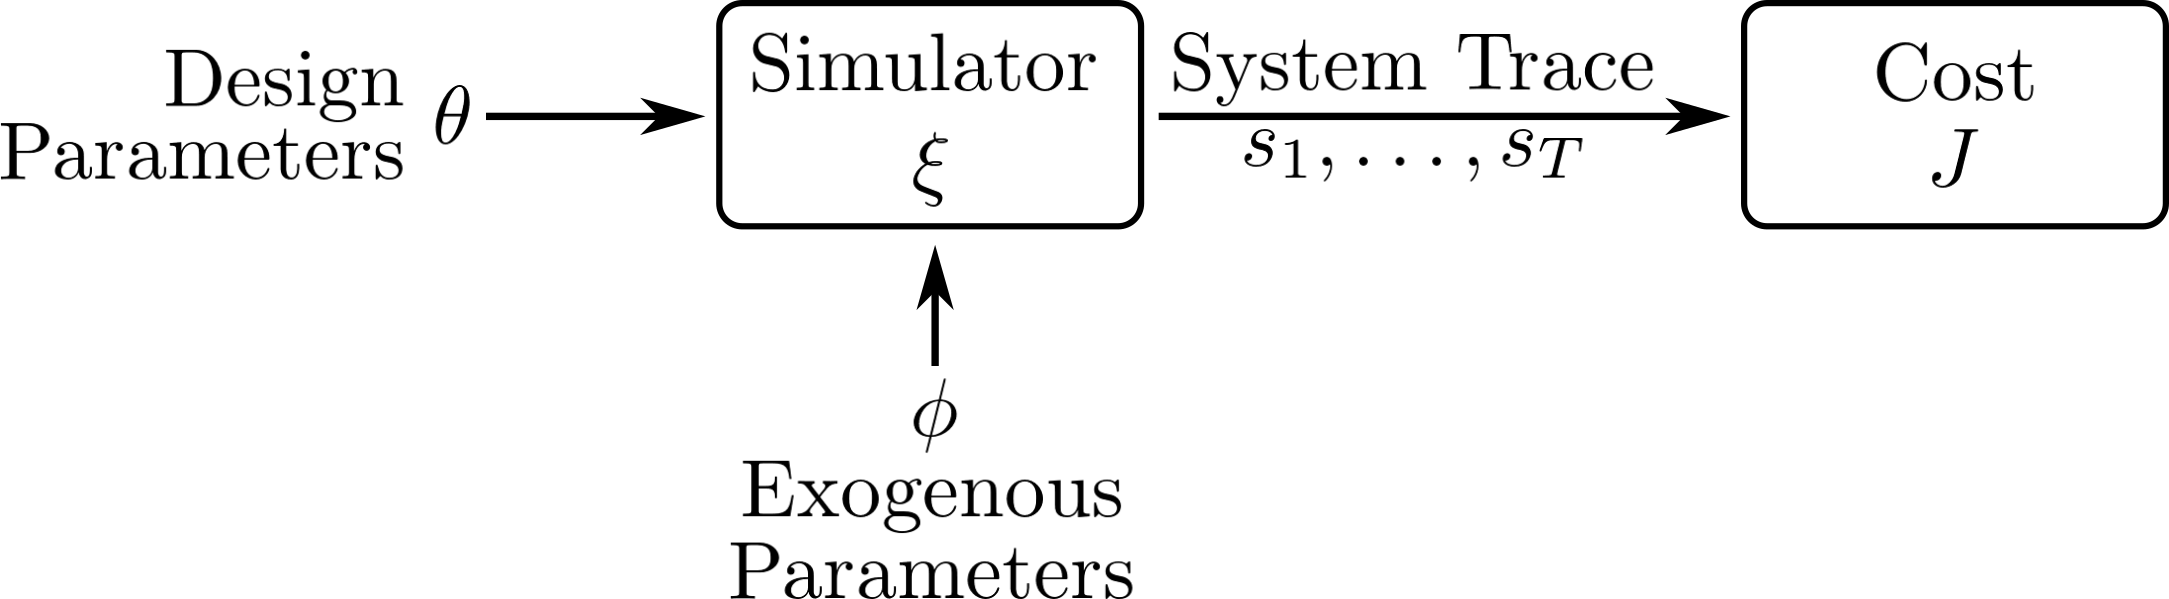
\includegraphics[width=\linewidth]{rss/block_diagram}
    \caption{A glass-box model of a generic robotic system. Design optimization involves finding a set of design parameters so that the simulated cost is minimized, while robustness analysis involves quantifying how changes in the exogenous parameters affect the simulated cost.}
    \label{ch:rss:fig:block_diagram}
\end{figure}

We can make this discussion concrete with an example: consider the autonomous ground vehicle (AGV) design problem illustrated in Fig.~\ref{ch:rss:fig:agv_example}. In this problem, our goal is to design a localization and navigation system that will allow the AGV to safely navigate between two obstacles. The AGV can estimate its position using an extended Kalman filter (EKF) with noisy measurements of its range from two nearby beacons and its heading from an IMU. The robot uses this estimate with a navigation function~\cite{aiama} and feedback controller to track a collision-free path between the obstacles.

In this problem, the design parameters $\theta$ include the $(x, y)$ locations of the two range beacons $b_1, b_2 \in \R^2$ and the feedback controller gains $k \in \R^2$. The exogenous parameters $\phi$ are the actuation and sensor noises at each timestep $w_t \in \R^3$ and $v_t \in \R^3$, drawn i.i.d. from Gaussian distributions $\mathcal{N}(0, Q)$ and $\mathcal{N}(0, R)$, respectively, as well as the initial state (also Gaussian). The simulator $\xi$ integrates the AGV's dynamics using a fixed timestep, updating the EKF and evaluating the navigation controller at each step. The cost function $J$ assigns a penalty to collisions with the environment, estimation errors, and deviations from the goal location. We will return to this example in more detail in Section~\ref{ch:rss:case1}; first, we discuss our approach to design optimization and robustness analysis in Sections~\ref{ch:rss:optimization} and~\ref{ch:rss:analysis}, respectively.

\begin{figure}[tb]
    \centering
    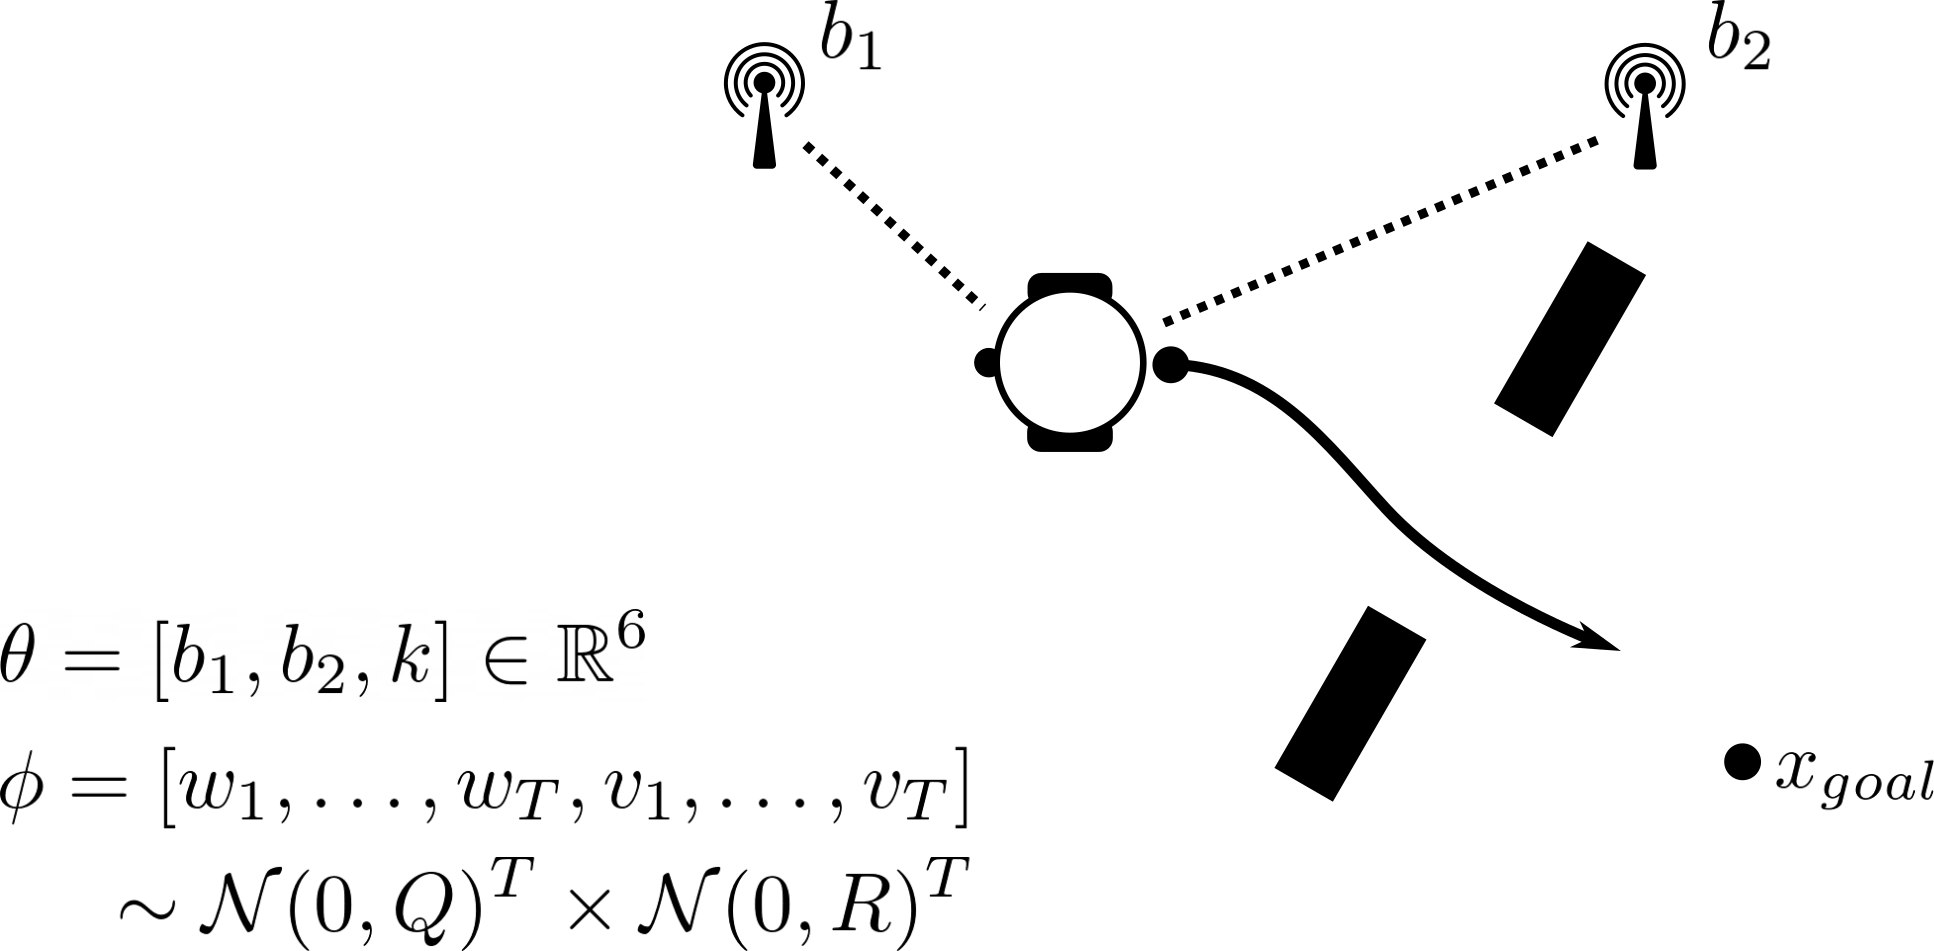
\includegraphics[width=0.8\linewidth]{rss/agv_example.png}
    \caption{A design optimization problem for an AGV localization and navigation system. The goal is to find placements for two range sensors along with parameters for the navigation system that allow the robot to safely pass through the narrow doorway.}
    \label{ch:rss:fig:agv_example}
\end{figure}

\section{Design optimization using differentiable programming}\label{ch:rss:optimization}

Given the notation from Section~\ref{ch:rss:prelim}, we can formally pose the robot design optimization problem. In formulating the optimization objective, it is important to consider the variance introduced by the exogenous parameters $\phi$. Simply minimizing the expected value of the cost $\expectation_{\phi \sim \Phi} \big[ J\circ S\pn{\theta, \phi} \big]$ (where $\circ$ denotes composition) can lead to myopic behavior where exceptional performance for some values of $\phi$ compensates for poor performance on other values; this is related to the phenomenon of ``reward hacking'' in reinforcement learning~\cite{amodei2016_ai_safety}.

Ideally, we would like our designs to be robust to variations in exogenous parameters: changing $\phi$ should not cause the performance to change much. We can include this requirement as a heuristic by penalizing the variance of $J$. Intuitively, this heuristic ``smooths'' the cost function with respect to the exogenous parameters: regions of high variance (containing sharp local minima) are penalized, while regions of low variance are rewarded. We return to justify this connection to robustness in Section~\ref{ch:rss:connection_to_robustness}. This heuristic leads us to the \textit{variance-regularized robust design optimization problem}:
\begin{subequations}\label{ch:rss:design_optimization_nlp_generic}
    \begin{align}
        \min_{\theta \in \Theta} & \quad \expectation_{\phi \sim \Phi} \Big[ J\circ S\pn{\theta, \phi} \Big] + \lambda \rm{Var}_{\phi\sim\Phi}\Big[ J\circ S\pn{\theta, \phi} \Big] \label{ch:rss:design_optimization_objective_generic} \\
        \text{s.t.}              & \quad c_i(\theta) \geq 0 \quad \forall i \in \mathcal{I}_c \label{ch:rss:design_optimization_constraints_generic}
    \end{align}
\end{subequations}
Practically, we replace the expectation and variance with unbiased estimates over $N$ samples $\phi_i \sim \Phi, i=1,\ldots,N$.
\begin{subequations}\label{ch:rss:design_optimization_nlp}
    \begin{align}
        \min_{\theta \in \Theta} & \quad \frac{1}{N}\sum_{i=1}^{N} \Big[J\circ S\pn{\theta, \phi_i}\Big] \label{ch:rss:design_optimization_objective}                                              \\
                                 & + \lambda \left[ \frac{\sum_{i=1}^N \pn{J\circ S\pn{\theta, \phi_i}}^2}{N-1} - \frac{\pn{\sum_{i=1}^N J\circ S\pn{\theta, \phi_i}}^2}{(N-1)N} \right] \nonumber \\
        \text{s.t.}              & \quad c_i(\theta) \geq 0 \quad \forall i \in \mathcal{I}_c \label{ch:rss:design_optimization_constraints}
    \end{align}
\end{subequations}

Of course, these Monte-Carlo estimates will require multiple evaluations of $J\circ S$ to evaluate~\eqref{ch:rss:design_optimization_objective}. Since $S$ might itself be expensive to evaluate, approximating the gradients of \eqref{ch:rss:design_optimization_objective} and \eqref{ch:rss:design_optimization_constraints} using finite differences will impose a large computational cost ($2nN$ additional evaluations of $J\circ S$ and $c_i$ at each step). Instead, we can turn to automatic differentiation (AD) to directly compute these gradients with respect to $\theta$, which we can use with any off-the-shelf gradient-based optimization algorithm. The precise choice of optimization algorithm is driven by the constraints and is not central to our framework. If the constraints are hyper-rectangle bounds on $\theta$, then algorithms like L-BFGS-B may be used, but if the constraints are more complex then sequential quadratic programming or interior-point methods may be used. Our implementation provides an interface to a range of optimization back-ends through SciPy~\cite{2020SciPy-NMeth}.

In this framework, the user need only implement the simulator and cost function for their specific problem using a differentiable programming framework like the JAX library for Python~\cite{jax2018github}, and this implementation can be used automatically for efficient gradient-based optimization. By implementing a library of additional building blocks in this AD paradigm (e.g. estimation algorithms like the EKF), we provide an AD-based design optimization tool that strikes a productive balance between flexibility and ease of use. At the time of this writing, this library of building blocks includes an EKF for state estimation, the dynamics of various common robot platforms, formal specification languages like signal temporal logic, and differentiable RGB and depth image rendering.

\section{Design certification via robustness analysis}\label{ch:rss:analysis}

Once we have found an optimal choice of design parameters, we need to verify that the design will be robust to uncertainty in the exogenous parameters. Similarly to 3D CAD and FEA packages for mechanical engineers, a successful design tool not only helps an engineer refine her design (i.e. using the design optimization framework in Section~\ref{ch:rss:optimization}) but also helps her analyze and predict its performance. To certify the performance of an optimized design, we are interested in two distinct questions. First, what is the maximum cost we can expect given variation in the exogenous parameters? Second, how sensitive is the cost to external disturbances: by how much can a change in the exogenous parameters increase the cost?

Answering these questions is difficult because we must extrapolate worst-case performance from a finite number of simulations. To address this difficulty, we develop a probabilistic approach based on extreme value theory in statistics~\cite{sridhar2021improving,wood_zhang_1996,coles_2001}. We begin by stating a relevant result:

\begin{theorem}[Extremal Types Theorem; 3.1.1 in ~\cite{coles_2001}]\label{ch:rss:extreme_value_thm}
    %
    Let $X_1, \ldots, X_N$ be random variables drawn i.i.d. from an unknown distribution and $M_N = \max_i \{ X_i \}$ be the sample maximum. If there exist sequences of normalizing constants $\{a_N > 0\}$ and $b_N$ such that the limiting distribution of $(M_N - b_N)/a_N$ as $N\to\infty$ is non-degenerate, then
    \begin{equation}
        \lim_{N\to\infty} \Pr\left[(M_N - b_N) / a_N \leq z \right] = G(z)
    \end{equation}
    where $G(z)$ is a Generalized Extreme Value Distribution (GEVD) with location $\mu$, scale $\sigma$, and shape $\xi$,
    \begin{equation}
        G(z) = \exp \left\{ -\left[ 1 + \xi\pn{\frac{z - \mu}{\sigma}} \right]^{-1/\xi} \right\},
    \end{equation}
    supported on $\{z : 1 + \xi(z - \mu)/\sigma > 0\}$.
\end{theorem}

In the special case $\xi = 0$, this distribution has a slightly different form (known as a Gumbel distribution), but the result holds. In practice, $a_n$ and $b_n$ are not estimated directly (this merely changes the fit values of $\mu$ and $\sigma$) and the GEVD is fit directly to $M_N$ by either maximizing the log likelihood~\cite{coles_2001} or estimating the posterior distribution of $(\mu, \sigma, \xi)$ using Markov Chain Monte Carlo methods~\cite{salvatier_wiecki_fonnesbeck_2016}. A useful feature of the GEVD is that if our data suggest that $\xi < 0$, then the support of $G(z)$ is bounded above and we can estimate an upper bound on the maximum $M_\infty$. If $\xi \geq 0$, then we cannot estimate a strict upper bound, but we can provide for a confidence interval for $M_\infty$ instead. In the following sections, we apply this theorem to analyze the robustness of an optimized design.

\subsection{Estimating the worst-case performance}

Our first robustness question concerns the worst-case performance of our design: given variation in $\phi$, what is the maximum cost we can expect for our choice of design parameters $\theta$? Our insight is that the variation $\phi \sim \Phi$ induces an (unknown) distribution in $J \circ S (\theta, \phi)$, so $J \circ S (\theta, \phi)$ a random variable to which the extremal types theorem applies. Algorithm~\ref{ch:rss:alg:worst_case_cost} provides a means for estimating the maximum of $J \circ S (\theta, \phi)$ by fitting a GEVD to observed maximums $M_N$. Generally speaking, the block size $N$ and sample size $M$ should be chosen to be as large as computationally feasible to reduce the variance of the GEVD estimate~\cite{coles_2001}.

\begin{algorithm}
    \caption{An algorithm for estimating the parameters of a GEVD governing the expected maximum cost $J \circ S$}\label{ch:rss:alg:worst_case_cost}
    \begin{algorithmic}
        \Require Block size $N > 0$ and sample size $M > 0$
        \State $X_j^i \gets J\circ S(\theta, \phi_{ij})$; with $\phi_{ij}\sim\Phi$, $1\leq j\leq N$, $1\leq i\leq M$
        \State $M_N^i \gets \max\{X_1^i, \ldots, X_N^i\}$ for $i=1,\ldots,M$
        \State $(\mu, \sigma, \xi) \gets$ posterior GEVD estimate given $\{M_N^i\}$
    \end{algorithmic}
\end{algorithm}

In practice, we use the automatic parallelization features of JAX to efficiently compute $X_j^i$ and obtain the posterior distribution of $\mu$, $\sigma$, and $\xi$ using Markov Chain Monte Carlo sampling with the PyMC3 library~\cite{salvatier_wiecki_fonnesbeck_2016}. From this posterior distribution, we take the $97\%$ confidence level for each parameter $(\mu^*, \sigma^*, \xi^*)$. If $\xi^* < 0$, we have confidence that the corresponding GEVD has bounded support on the right and estimate the maximum cost $J_{max} \leq \mu - \sigma/\xi$. Otherwise, we can estimate the 97\% confidence level for $J_{max}$ using the GEVD described by $(\mu^*, \sigma^*, \xi^*)$.

\subsection{Estimating sensitivity}

In addition to the expected worst-case performance, it is also useful to know the sensitivity of that performance. That is, if the design performs well in one situation (i.e. for some value of $\phi$), then how much can we expect its performance to degrade if $\phi$ changes? Formally, we define the sensitivity $L$ as the least constant such that for any two $\phi_1, \phi_2 \sim \Phi$, $$|J\circ S(\theta, \phi_1) - J\circ S(\theta, \phi_2)| \leq L ||\phi_1 - \phi_2||$$
If $J \circ S$ is Lipschitz then $L$ will be finite and equal the Lipschitz constant of $J \circ S$, but we do not require this assumption; if $J \circ S$ is not Lipschitz, then we can estimate a high-confidence upper bound on $L$.

In both cases, we can exploit the fact that $L$ is an extreme value of the slope $|J\circ S(\theta, \phi_1) - J\circ S(\theta, \phi_2)| / ||\phi_1 - \phi_2||$ and apply the extremal types theorem. Let $X = ||J\circ S(\theta, \phi_1) - J\circ S(\theta, \phi_2)|| / ||\phi_1 - \phi_2||$ be a random variable with $\phi_1, \phi_2 \sim \Phi$. The distribution of $X$ is unknown, but the extremal types theorem lets us characterize the sample maximum $L_N = \max\{X_1, \ldots, X_N\}$ using a GEVD. Algorithm~\ref{ch:rss:alg:sensitivity} provides our method for fitting this distribution. This approach is similar to that in~\cite{sridhar2021improving,knuthPlanningLearnedDynamics2021} but removes the assumption that $L$ is bounded by fitting a GEVD instead of a reverse Weibull distribution, allowing our approach to apply even when $J\circ S$ is not Lipschitz.
\begin{algorithm}
    \caption{An algorithm for estimating the parameters of a GEVD governing the sensitivity of $J \circ S$}\label{ch:rss:alg:sensitivity}
    \begin{algorithmic}
        \Require Block size $N > 0$ and sample size $M > 0$
        \State $X_j^i \gets |J\circ S(\theta, \phi_{ij,1}) - J\circ S(\theta, \phi_{ij,2})| / ||\phi_{ij,1} - \phi_{ij,2}||$, \hspace{2cm} \phantom{xxxxxxx} with $\phi_{ij,1}, \phi_{ij,2} \sim\Phi$, $j=1,\ldots,N$, $i=1,\ldots,M$
        \State $L_N^i \gets \max\{X_1^i, \ldots, X_N^i\}$ for $i=1,\ldots,M$
        \State $(\mu, \sigma, \xi) \gets$ posterior GEVD estimate given $\{L_N^i\}$
    \end{algorithmic}
\end{algorithm}

Algorithm~\ref{ch:rss:alg:sensitivity} is similar to Algorithm~\ref{ch:rss:alg:worst_case_cost}, but the interpretation of the results differs in that Algorithm~\ref{ch:rss:alg:sensitivity} allow us to understand the sensitivity of a design rather than its worst-case performance. In particular, if the 97\% confidence level for the shape parameter $\xi^*$ is negative, then $J\circ S$ is likely Lipschitz continuous with Lipschitz constant $L \leq \mu - \frac{\sigma}{\xi}$. If $\xi > 0$, then $J\circ S$ is likely not Lipschitz but we can estimate the 97\% confidence level for $L$. As a result, this statistical approach allows us to avoid making prior assumptions about the continuity of our system.

\subsection{Theoretical connections between verification by extremal types and variance-regularized optimization}\label{ch:rss:connection_to_robustness}

Here, we will attempt to justify the variance regularization heuristic introduced in Section~\ref{ch:rss:optimization} with reference to the worst-case performance $J_{max}$ and sensitivity $L$ computed by Algorithms~\ref{ch:rss:alg:worst_case_cost} and~\ref{ch:rss:alg:sensitivity}. First, let us examine the connection with expected worst-case performance $J_{max}$. If we take the probability of observing a cost $J = J\circ S(\theta, \phi)$ within $\alpha$ of $J_{max}$, with $0 < \alpha < 1$, and apply Cantelli's inequality~\cite{boucheron_lugosi_massart_2016}, we see that
\begin{align*}
    % \rm{Pr}_{\phi \sim \Phi}(J \geq \alpha J_{max}) &= \rm{Pr}\pn{J \geq \expectation_{\phi \sim \Phi}[J] + (\alpha J_{max} - \expectation_{\phi \sim \Phi}[J])} \\
    \rm{Pr}_{\phi \sim \Phi}(J \geq \alpha J_{max}) & \leq \frac{\rm{Var}_{\phi \sim \Phi}[J]}{\rm{Var}_{\phi \sim \Phi}[J] + (\alpha J_{max} - \expectation_{\phi \sim \Phi}[J])^2}
\end{align*}
Minimizing $\rm{Var}_{\phi \sim \Phi}[J]$ in addition to $\expectation_{\phi \sim \Phi}[J]$ will correlate with decreasing this upper bound. As a result, we expect variance regularization to correlate with decreased probability of encountering near-worst-case performance.

We can also justify the connection between variance regularization and reducing sensitivity $L$ by looking at the special case where $J \circ S$ is Lipschitz and the elements of $\phi$ are independent. The Bobkov-Houdr\'e variance bound for Lipschitz functions~\cite{bobkov} holds that $\rm{Var}_{\phi \sim \Phi}[J] \leq L^2 \sigma_{\Sigma\phi}^2$,
where $\sigma_{\Sigma\phi}^2$ is the variance of the sum of elements in $\phi$. This bound does not guarantee that minimizing $\rm{Var}_{\phi \sim \Phi}[J]$ decreases $L$, but it suggests a correlation between these quantities.

\section{Experimental results}\label{ch:rss:cases}

So far, we have developed the theoretical and algorithmic basis for our robot design framework. It remains for us to empirically answer two questions: first, is our framework useful for solving practical robot design problems? Second, is our statistical method for robustness analysis sound?

In this section, we answer these questions through the lens of two case studies. The first involves finding optimal sensor placements for robot navigation, and the second involves optimizing a pushing strategy for multi-agent manipulation. We demonstrate the success of our optimization and robustness analysis framework on each example, and we provide results from hardware testing in both cases. Next, we include an ablation study justifying our use of automatic differentiation and variance regularization. We conclude by verifying the soundness of our statistical robustness analysis.

\subsection{Case study: optimal sensor placement for navigation}\label{ch:rss:case1}

First, we return to the AGV localization and navigation example introduced in Fig.~\ref{ch:rss:fig:agv_example}. This design problem requires finding an optimal placement for two ranging beacons to minimize estimation error and allow the robot to safely navigate between two obstacles. Range measurements from these beacons are integrated with IMU data via an EKF, and the resulting state estimate is used as input to a navigation function and tracking feedback controller to guide the robot to its goal. This design problem has two important features. First, it involves interactions between multiple subsystems: the output from the EKF is used by the navigation function, which feeds input to the controller, which in turn influences future EKF predictions. Second, the effect of uncertainty on the robot's performance is relatively strong.

The design parameters are the $(x, y)$ locations of two range beacons and two feedback controller gains (6 total design parameters). The exogenous parameters include uncertainty in the robot's initial state along with actuation and sensing noise at each of $T$ timesteps ($3 + 6T$ total exogenous parameters). The cost function has three components: one penalizing large estimation errors, one penalizing deviations from the goal, and one penalizing collisions with the environment. A formal definition of the design and exogenous parameters, simulator, cost, and constraints is given in Table~\ref{ch:rss:tab:agv_design_problem} in the appendix. The simulator and cost functions are implemented in Python using the JAX framework for automatic differentiation.

Fig.~\ref{ch:rss:fig:agv_representative_trajectories} compares simulated trajectories for the initial and optimized beacon placements and feedback gains, clearly showing the impact of design optimization. Initially, poor beacon placement causes the robot to accumulate estimation error and drift away from its goal. The optimized design moves the beacons off to the side to eliminate this drift. Optimization ($N=512$, $\lambda=0.1$, L-BFGS-B back-end) takes 3 minutes \SI{34}{s} on a laptop computer (\SI{8}{GB} RAM, \SI{1.8}{GHz} 8-core processor).

We test the initial and optimized design in hardware using the Turtlebot 3 platform. To emulate range beacon measurements in our lab, odometry and laser scan data are fused into a full state estimate from which range measurements are derived (the full state estimate is hidden from the robot, which only received the emulated range measurements). The control frequency is increased from \SI{2}{Hz} in simulation to \SI{10}{Hz} in hardware, and the obstacles are recreated in our laboratory. The hardware results, shown in Figs.~\ref{ch:rss:fig:agv_hw} and~\ref{ch:rss:fig:agv_hw_cov}, confirm our simulation results: the initial design suffers from drift and ends approximately \SI{10}{cm} from its target position, while the optimized design does not drift and ends within \SI{5}{cm} of the goal. This difference can be seen most clearly in the posterior error covariance from the EKF;  Fig.~\ref{ch:rss:fig:agv_hw_cov} shows how the optimized design greatly reduces uncertainty in the state estimate compared to the initial design. No parameter estimation or tuning on hardware was required.

\begin{figure}[tb]
    \centering
    \begin{subfigure}[c]{0.45\linewidth}
        \centering
        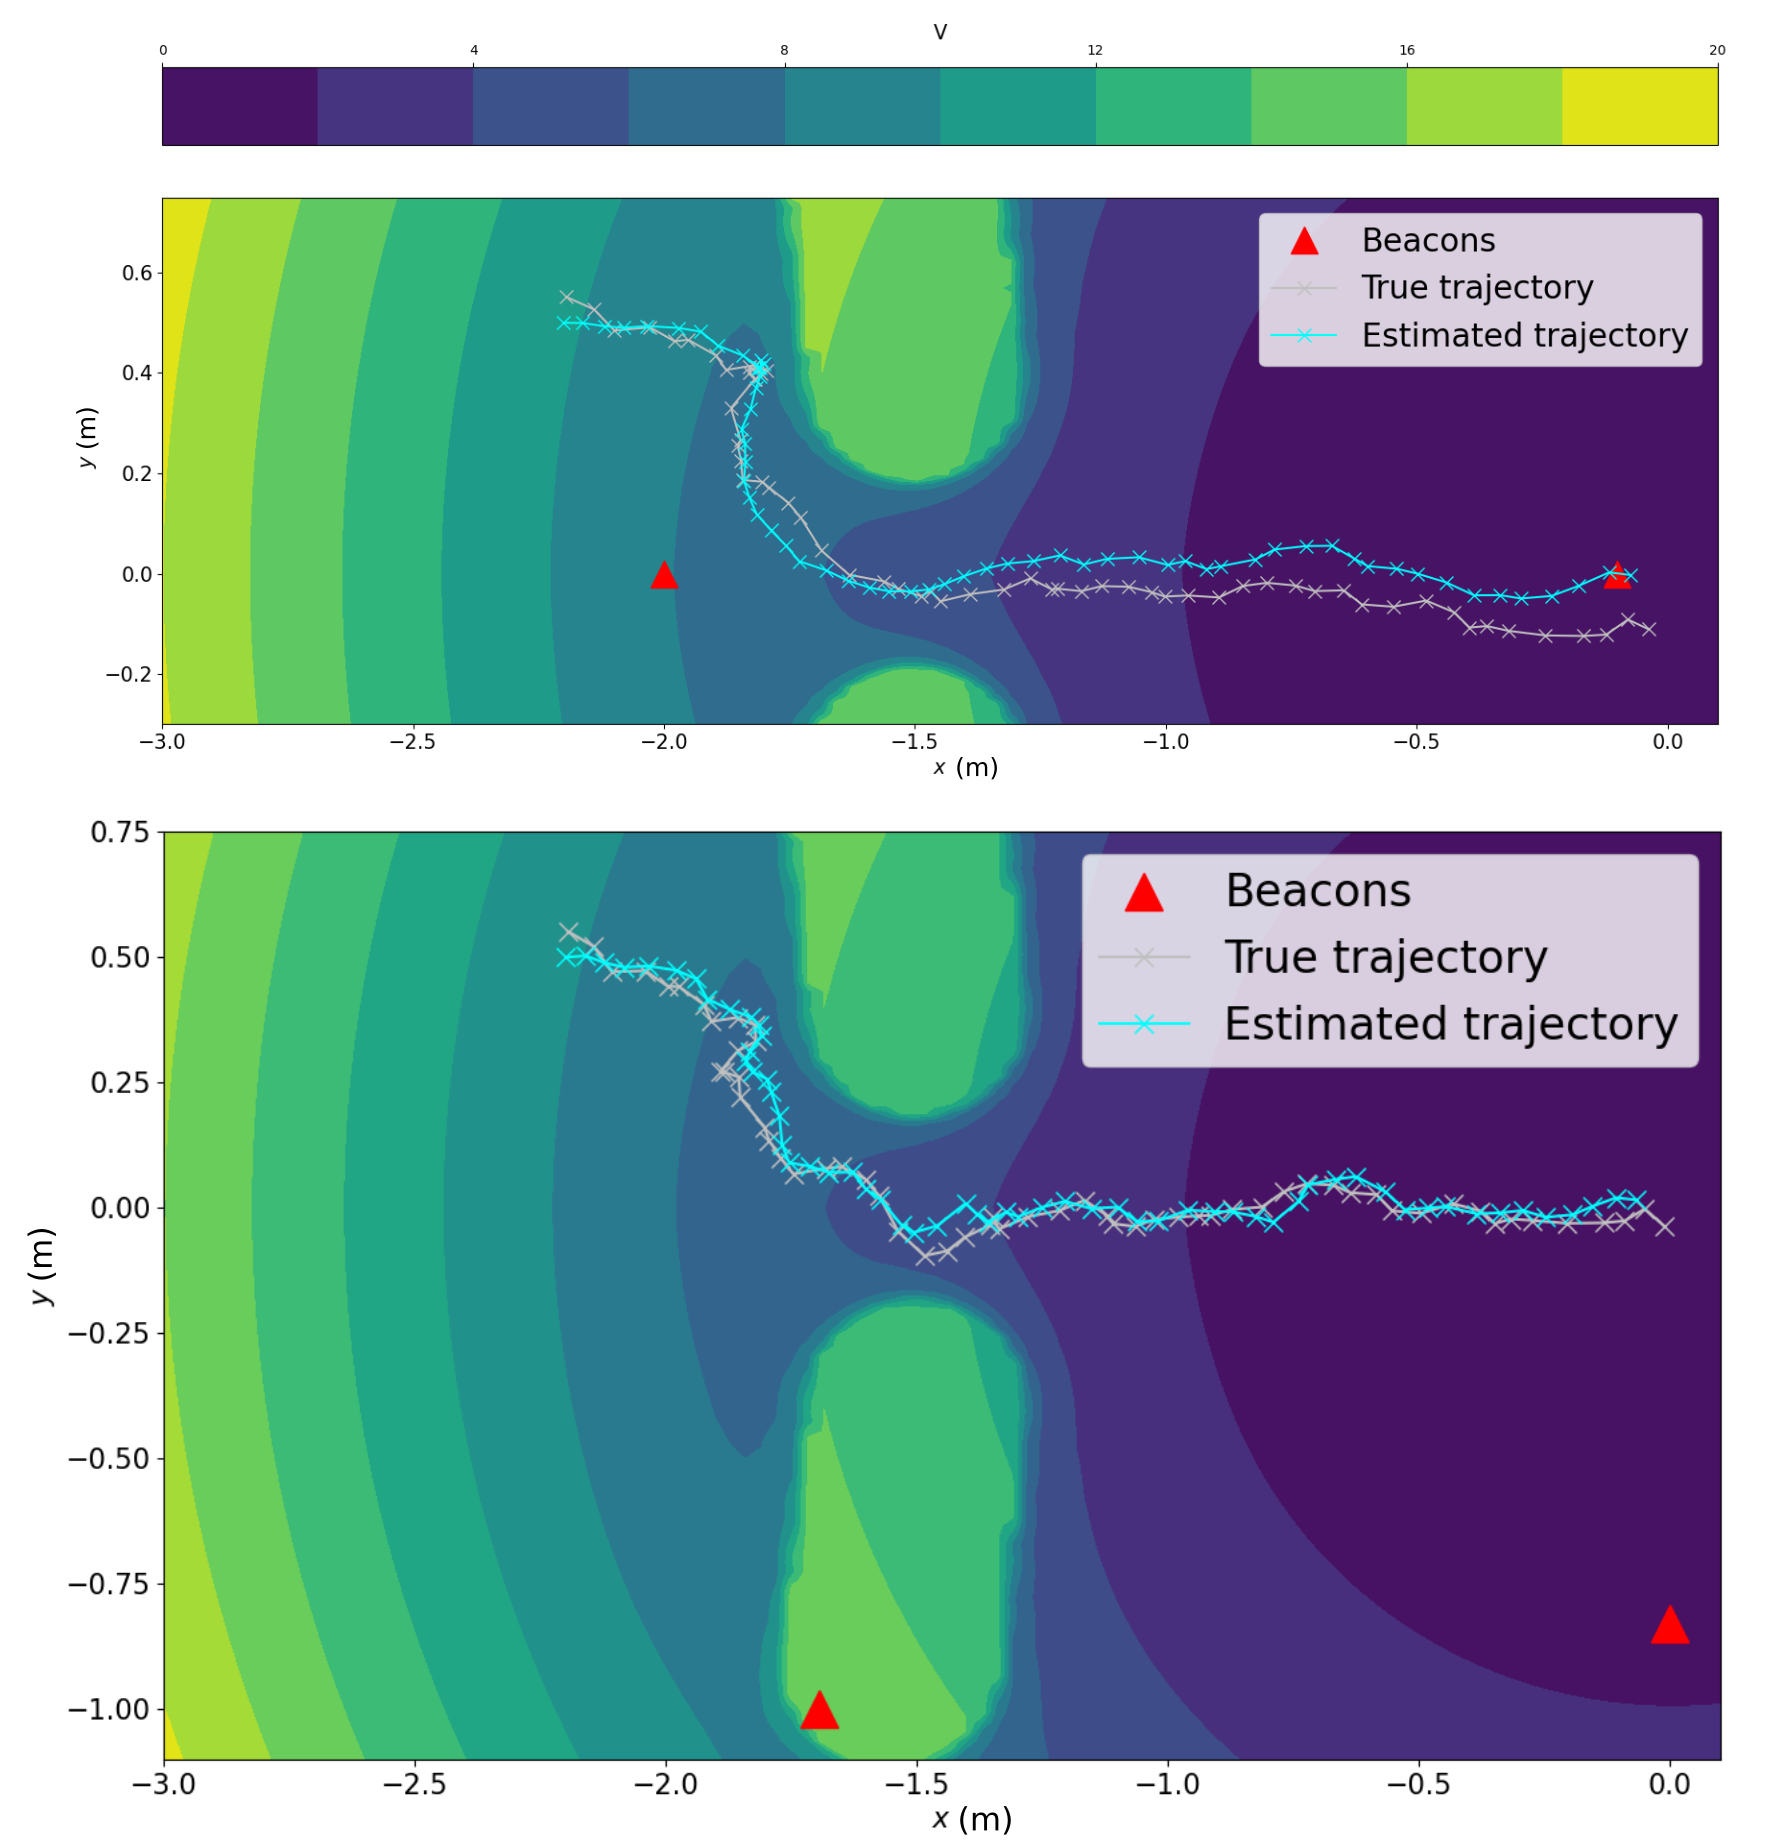
\includegraphics[width=\linewidth]{rss/agv_simulation_stacked.png}
        \caption{Simulated trajectories for the initial (top) and optimized (bottom) AGV designs. Navigation function contours are shown in color.}
        \label{ch:rss:fig:agv_representative_trajectories}
    \end{subfigure}
    \quad
    \begin{subfigure}[c]{0.45\linewidth}
        \begin{subfigure}[t]{\linewidth}
            \centering
            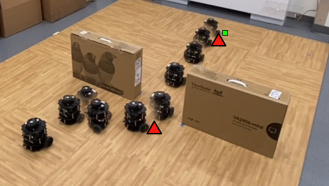
\includegraphics[width=\linewidth]{rss/agv_initial_composite.png}
        \end{subfigure}

        \begin{subfigure}[t]{\linewidth}
            \centering
            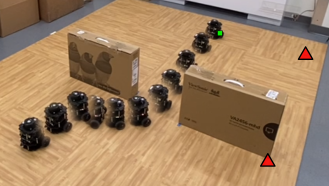
\includegraphics[width=\linewidth]{rss/agv_optimized_composite.png}
        \end{subfigure}
        \caption{Hardware performance of initial (top) and optimized (bottom) AGV designs. Square (green) shows the goal; triangles (red) show beacon locations. The optimized design eliminates drift relative to goal.}
        \label{ch:rss:fig:agv_hw}
    \end{subfigure}
\end{figure}

We then apply the robustness analysis from Section~\ref{ch:rss:analysis} to certify the maximum absolute estimation error $\norm{x_t - \hat{x}_t}$ in the optimized design (in meters, projected into the $xy$ plane). Note that this error is different from the cost used during optimization, but we can still apply Algorithm~\ref{ch:rss:alg:worst_case_cost} simply by changing the cost function for the duration of the analysis. Using block size $N = 1000$ and sample size $M = 1000$, we fit a GEVD using Algorithm~\ref{ch:rss:alg:worst_case_cost} to the maximum estimation error for both the initial and optimized designs. These distributions are shown in Fig.~\ref{ch:rss:fig:agv_gevd}; the optimized design significantly reduces the expected maximum estimation error. We observe that the 97\% confidence level for the shape parameter $\xi = 0.059$ is positive, so we cannot conclude that the worst-case estimation error is bounded, but we can derive a high-confidence bound of \SI{0.21}{m} for our optimized design.

\begin{figure}[tb]
    \centering
    \begin{subfigure}[c]{0.45\linewidth}
        \centering
        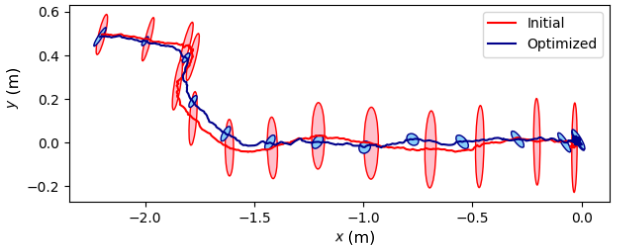
\includegraphics[width=\linewidth]{rss/agv_hw_covariance.png}
        \caption{Hardware results for EKF state estimates and posterior error covariance $3\sigma$ ellipse for initial and optimized AGV designs.}
        \label{ch:rss:fig:agv_hw_cov}
    \end{subfigure}
    \quad
    \begin{subfigure}[c]{0.45\linewidth}
        \centering
        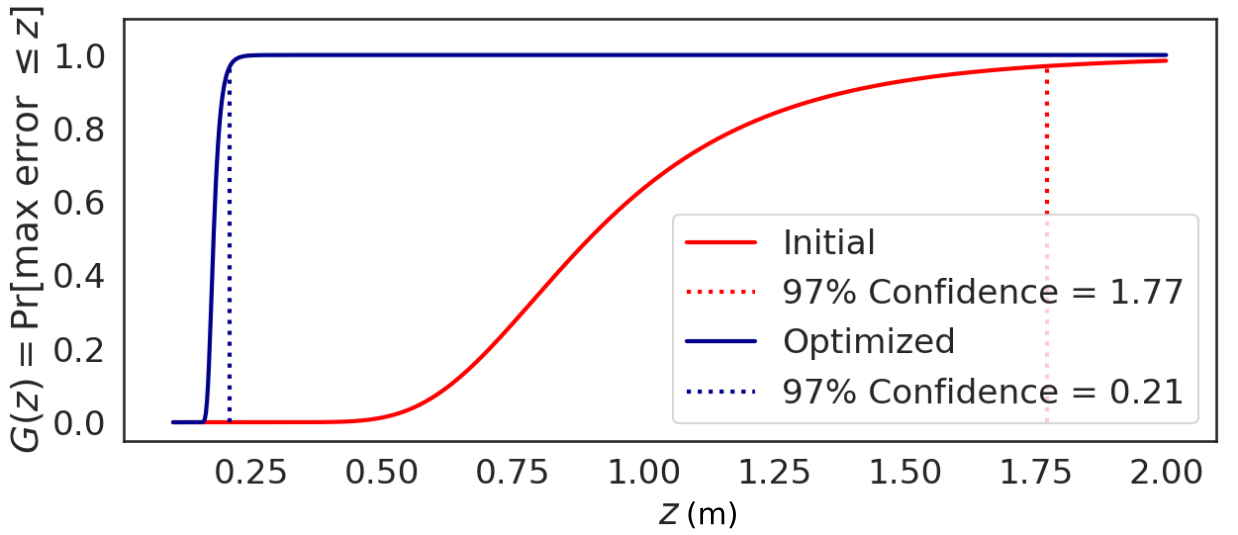
\includegraphics[width=\linewidth]{rss/agv_worst_case_error.png}
        \caption{GEVD CDF fit using Algorithm~\ref{ch:rss:alg:worst_case_cost} for the maximum absolute estimation error in the $xy$-plane in both the initial and optimized AGV designs, with 97\% confidence levels.}
        \label{ch:rss:fig:agv_gevd}
    \end{subfigure}
\end{figure}

\subsection{Case study: collaborative multi-robot manipulation}\label{ch:rss:case2}

Our second example involves finding a control strategy for multi-agent collaborative manipulation. In this setting, two ground robots must collaborate to push a box from its current location to a target pose (as in Fig.~\ref{ch:rss:fig:mam_example}). Given the desired box pose and the current location of each robot, a neural network plans a trajectory for each robot, which the robots then track using a feedback controller ($\theta$ includes both the neural network parameters and the tracking controller gains, with a total of 454 design parameters). The exogenous parameters include the coefficient of friction for each contact pair, the mass of the box, the desired pose of the box, and the initial pose for each robot (a total of 13 exogenous parameters; we vary the desired box pose and initial robot poses to prevent over-fitting during optimization). The cost function is simply the squared error between the desired box pose (including position and orientation) and its true final pose after a \SI{4}{s} simulation. A full definition of this design problem and contact dynamics model is included in Table~\ref{ch:rss:tab:mam_design_problem} in the appendix. We implement the contact dynamics simulator, trajectory planning neural network, and path tracking controller in Python using JAX.

\begin{figure}[tb]
    \centering
    \begin{subfigure}[c]{0.45\linewidth}
        \centering
        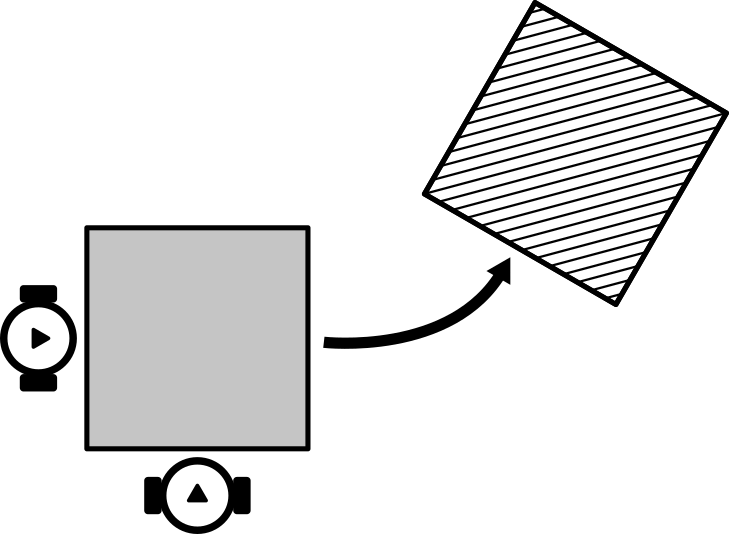
\includegraphics[width=0.7\linewidth]{rss/mam_example.png}
        \caption{Multi-agent manipulation design optimization problem. The goal is to find parameters for robot controllers and a neural network planner that push the box from an initial position (solid) to a desired position (striped).}
        \label{ch:rss:fig:mam_example}
    \end{subfigure}
    \quad
    \begin{subfigure}[c]{0.45\linewidth}
        \centering
        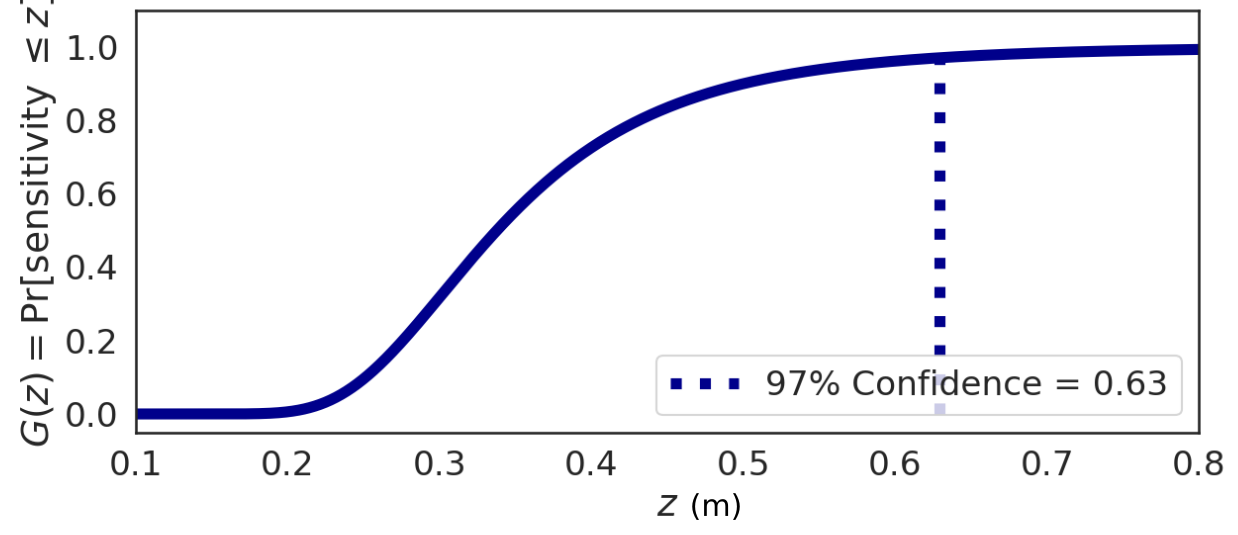
\includegraphics[width=0.8\linewidth]{rss/mam_sensitivity_friction.png}
        \caption{GEVD CDF fit using Algorithm~\ref{ch:rss:alg:sensitivity} for the maximum sensitivity of the optimized collaborative manipulation strategy to variation in friction coefficient. $z$ has units of meters per unit change in friction coefficient.}
        \label{ch:rss:fig:mam_gevd}
    \end{subfigure}
\end{figure}

\begin{figure}[tb]
    \centering
    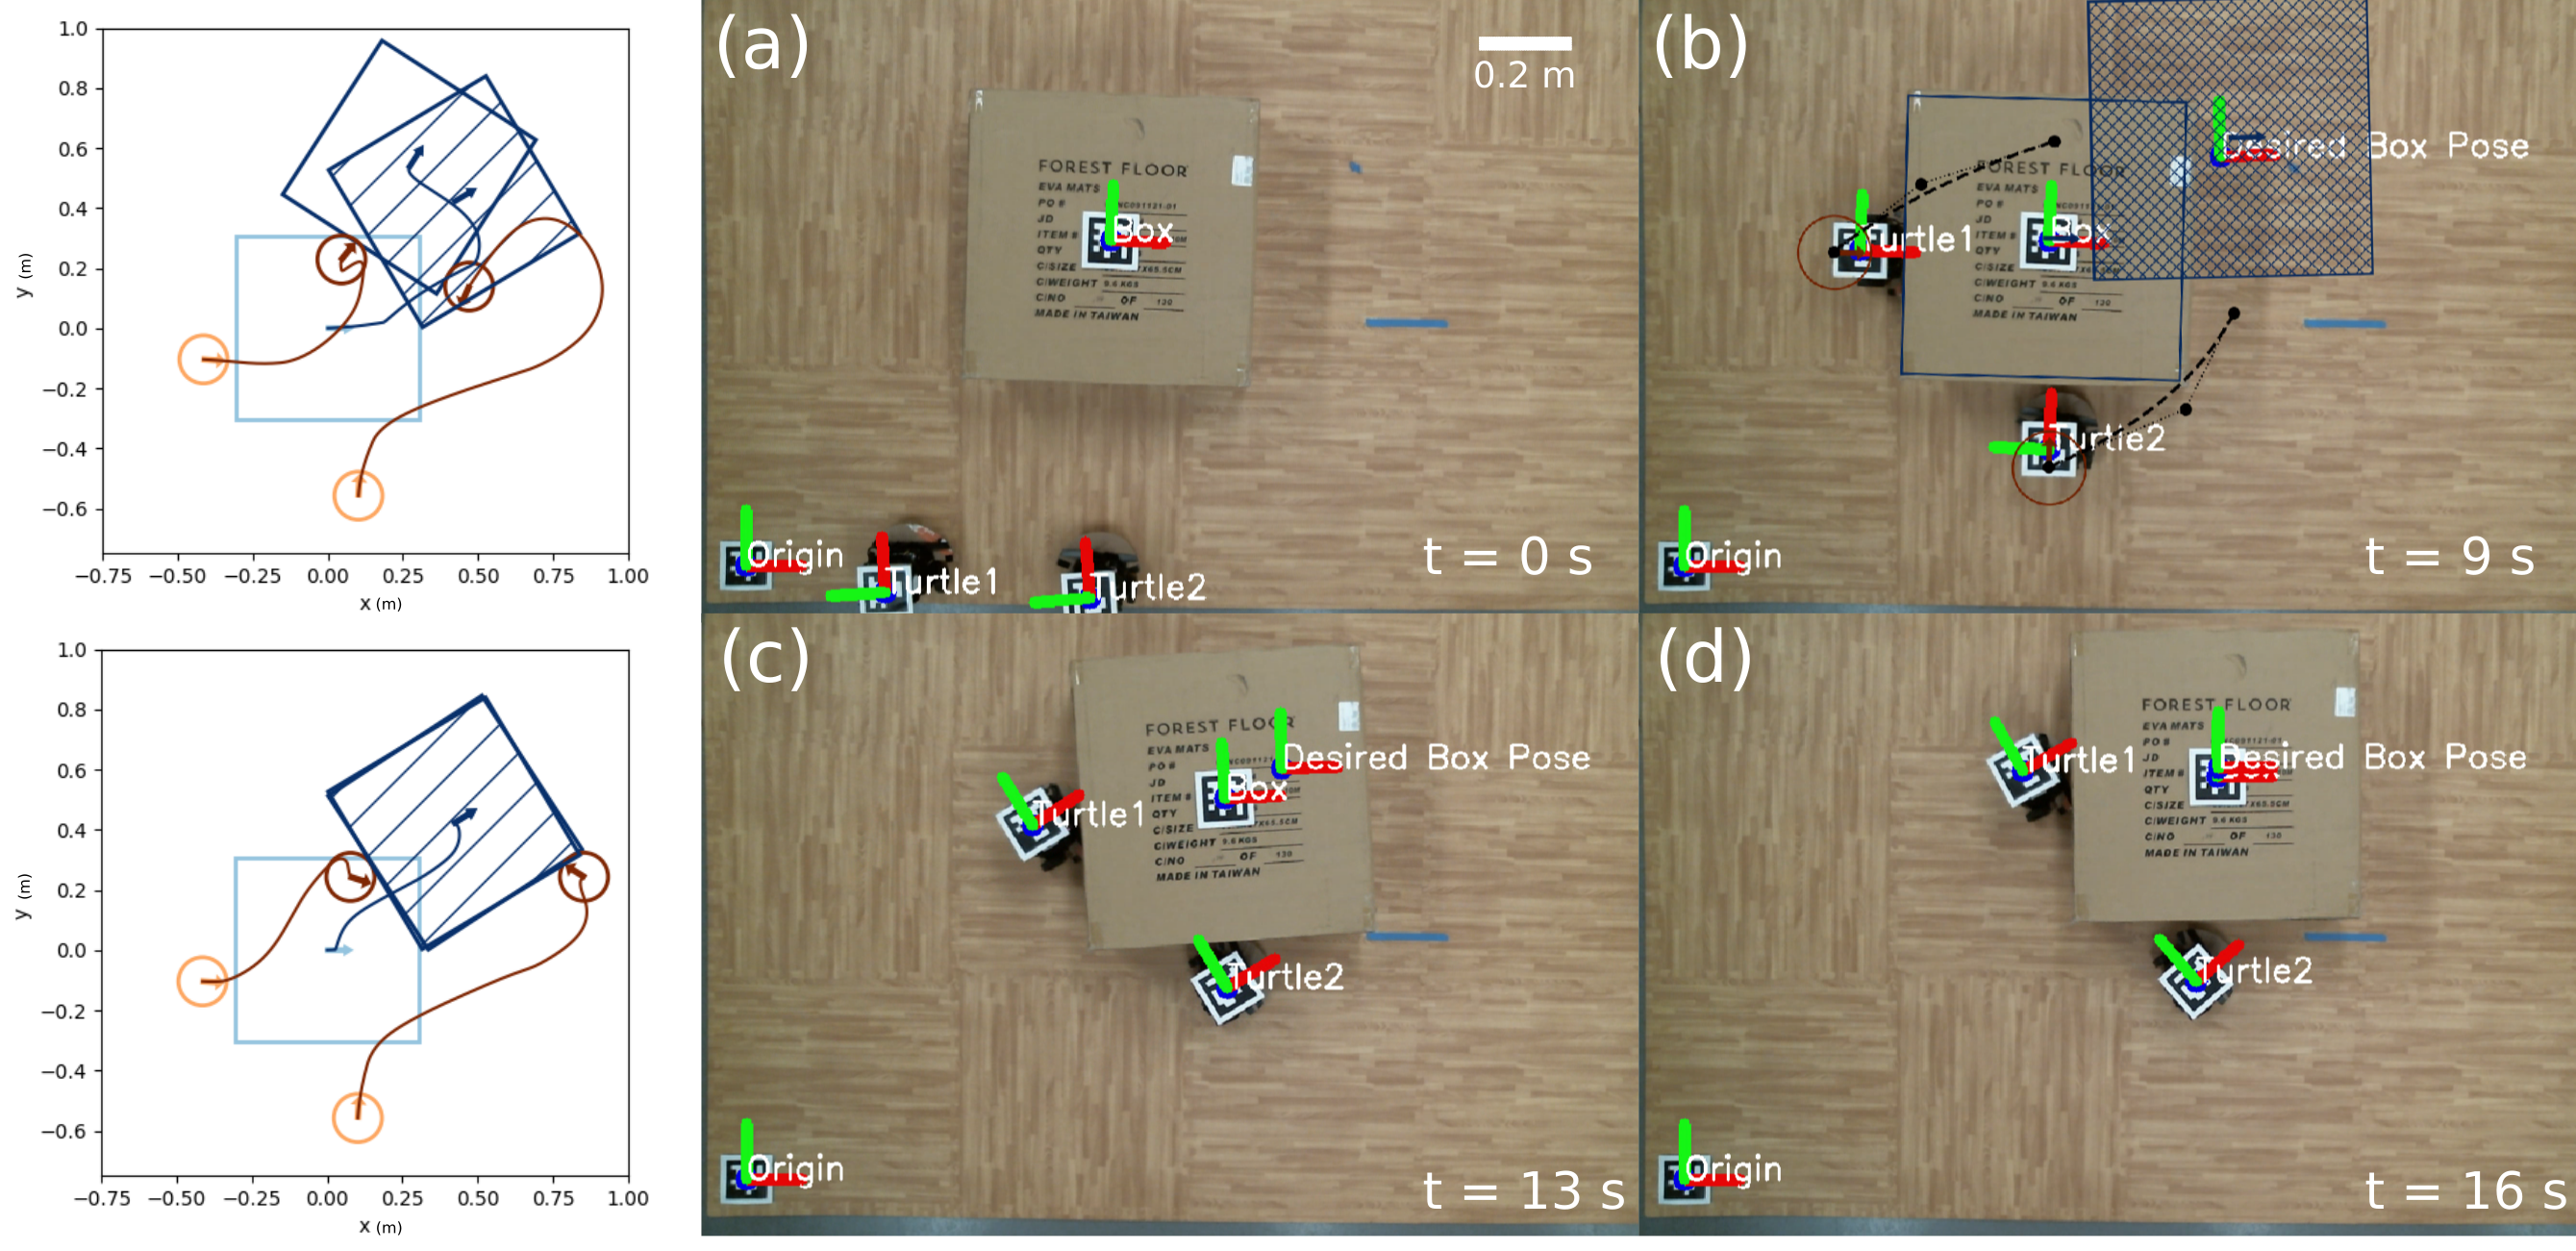
\includegraphics[width=\linewidth]{rss/mam_composite_w_sim.png}
    \caption{Left: Initial (top) and optimized (bottom) manipulation strategies in simulation (light/dark colors indicate initial/final positions, stripes indicate desired position). Right: Optimized manipulation strategy deployed in hardware. (a) The robots first move to positions around the box. (b) Using the optimized neural network, the robots plan a cubic spline trajectory pushing the box to its desired location. (c-d) The robots execute the plan by tracking that trajectory.}
    \label{ch:rss:fig:mam_hw}
\end{figure}


% \begin{figure}[tb!]
%     \centering
%     \begin{subfigure}[t]{0.4\linewidth}
%         \centering
%         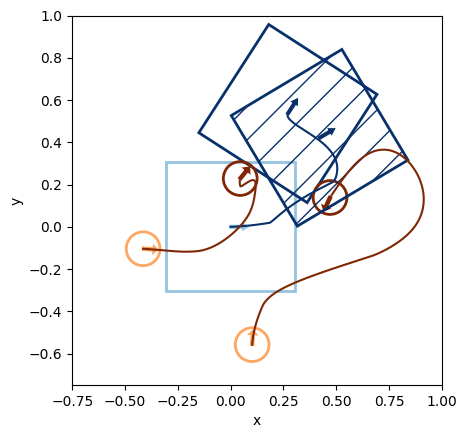
\includegraphics[width=\linewidth]{rss/mam_initial_traj.png}
%     \end{subfigure}%
%     \begin{subfigure}[t]{0.4\linewidth}
%         \centering
%         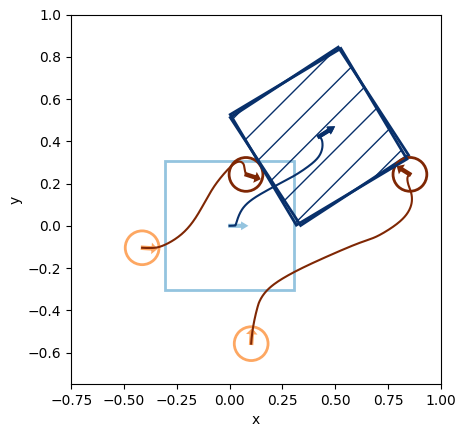
\includegraphics[width=\linewidth]{rss/mam_optimized_traj.png}
%     \end{subfigure}
%     \caption{Simulated initial (left) and optimized (right) manipulation strategies. Light/dark colors indicate initial/final positions, respectively. The striped box indicates the desired position.}
%     \label{ch:rss:fig:mam_sim}
% \end{figure}

Compared to the design problem in our first case study, this system has a simpler architecture (fewer subsystems) but more complicated dynamics and a much higher-dimensional design space. This example also showcases a different interpretation of the exogenous parameters: instead of representing true sources of randomness, these parameters represent quantities that are simply unknown at design-time. For example, the target position for the box is not random in the same way as sensor noise in the previous example, but since we cannot choose this value at design-time it must be included in $\phi$. As a result, minimizing the expected cost with respect to variation in $\phi$ yields a solution that achieves good performance for many different target poses, enabling the user to select one at run-time and be confident that the design will perform well.

To solve this design problem, the neural network parameters are initialized i.i.d. according to a Gaussian distribution, and the tracking controller gains are set to nominal values. We then optimize the parameters using $N = 512$, $\lambda = 0.1$, and L-BFGS-B back-end. This optimization took 45 minutes \SI{32}{s} on a laptop computer (\SI{8}{GB} of RAM and a \SI{1.8}{GHz} 8-core processor). Fig.~\ref{ch:rss:fig:mam_hw} shows a comparison between the initial and optimized strategies, and Fig.~\ref{ch:rss:fig:mam_more} in the appendix shows additional examples of the optimized behavior. The target pose is drawn uniformly $[x, y, \theta] \in[0, 0.5]^2 \times [-\pi/4, \pi/4]$, and the optimized design achieves a mean squared error of $0.0964$.

We test the optimized design in hardware, again using the Turtlebot 3 platform. An overhead camera and AprilTag~\cite{olson2011tags} markers are used to obtain the location of the box and each robot. At execution, each robot first moves to a designated starting location near the box, plans a trajectory using the neural network policy, and tracks that trajectory at \SI{100}{Hz} until the box reaches its desired location or a time limit is reached. Results from this hardware experiment are shown in Fig.~\ref{ch:rss:fig:mam_hw}. Again, no parameter tuning or estimation on hardware was needed.

After successfully testing the optimized design in the laboratory, it is natural to ask how its performance might change as conditions (particularly the coefficients of friction) change. Using $M = 500$ blocks of size $N=1000$ each, we use Algorithm~\ref{ch:rss:alg:sensitivity} to fit a GEVD for the sensitivity constant $L$ with respect to the coefficients of friction between each contact pair. We do this by allowing these coefficients to vary and freezing other elements of $\phi$ at nominal values (box mass \SI{1}{kg} and target pose $[0.3, 0.3, 0.3]$). The fit distribution is shown in Fig.~\ref{ch:rss:fig:mam_gevd}. The 97\% confidence level for the shape parameter is $\xi = 0.118 > 0$, so we cannot conclude that the performance of our design is Lipschitz with respect to the friction coefficients, but we can estimate the 97\% confidence level for $L$ as $0.63$.


\begin{figure}[t]
    \centering
    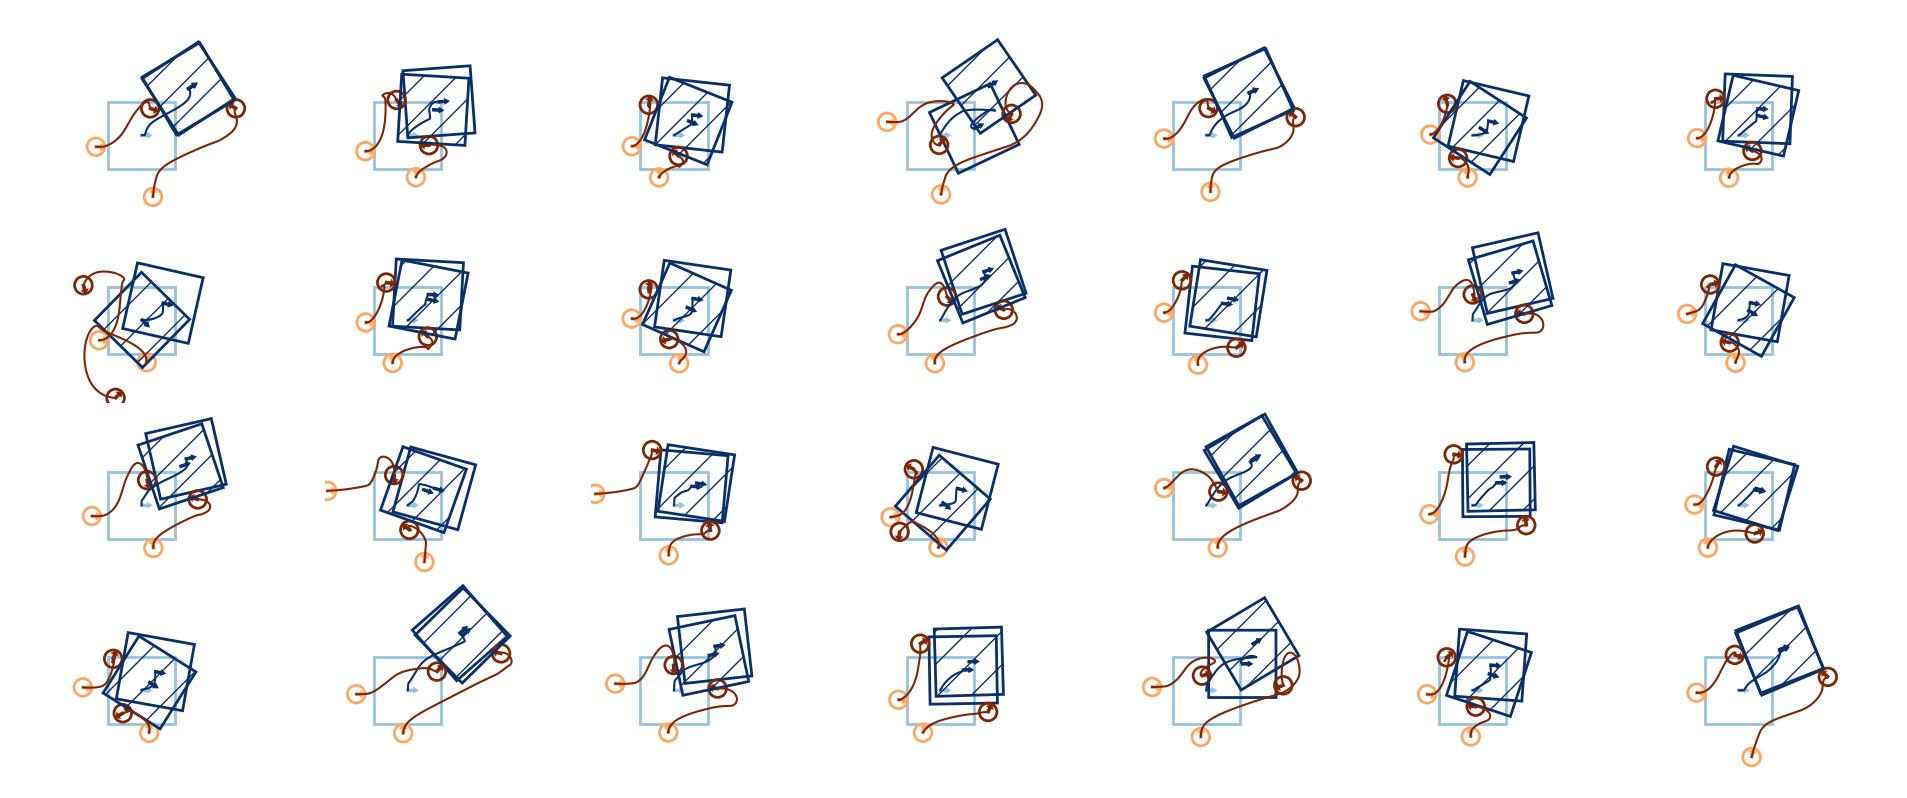
\includegraphics[width=\linewidth]{rss/mam_more.png}
    \caption{Additional examples of optimized multi-agent manipulation behavior in simulation, showing that the optimized strategy reaches the goal in most cases. Each example shows the results of executing the optimized pushing strategy for \SI{4}{s} with a randomly selected set of friction coefficients, random target pose, and random initial robot poses. Light/dark colors indicate initial/final positions, respectively, and the striped box indicates the target pose.}
    \label{ch:rss:fig:mam_more}
\end{figure}


\subsection{Design optimization ablation study}\label{ch:rss:ablation}

\begin{figure}[t]
    \centering
    \begin{subfigure}[t]{0.45\linewidth}
        \centering
        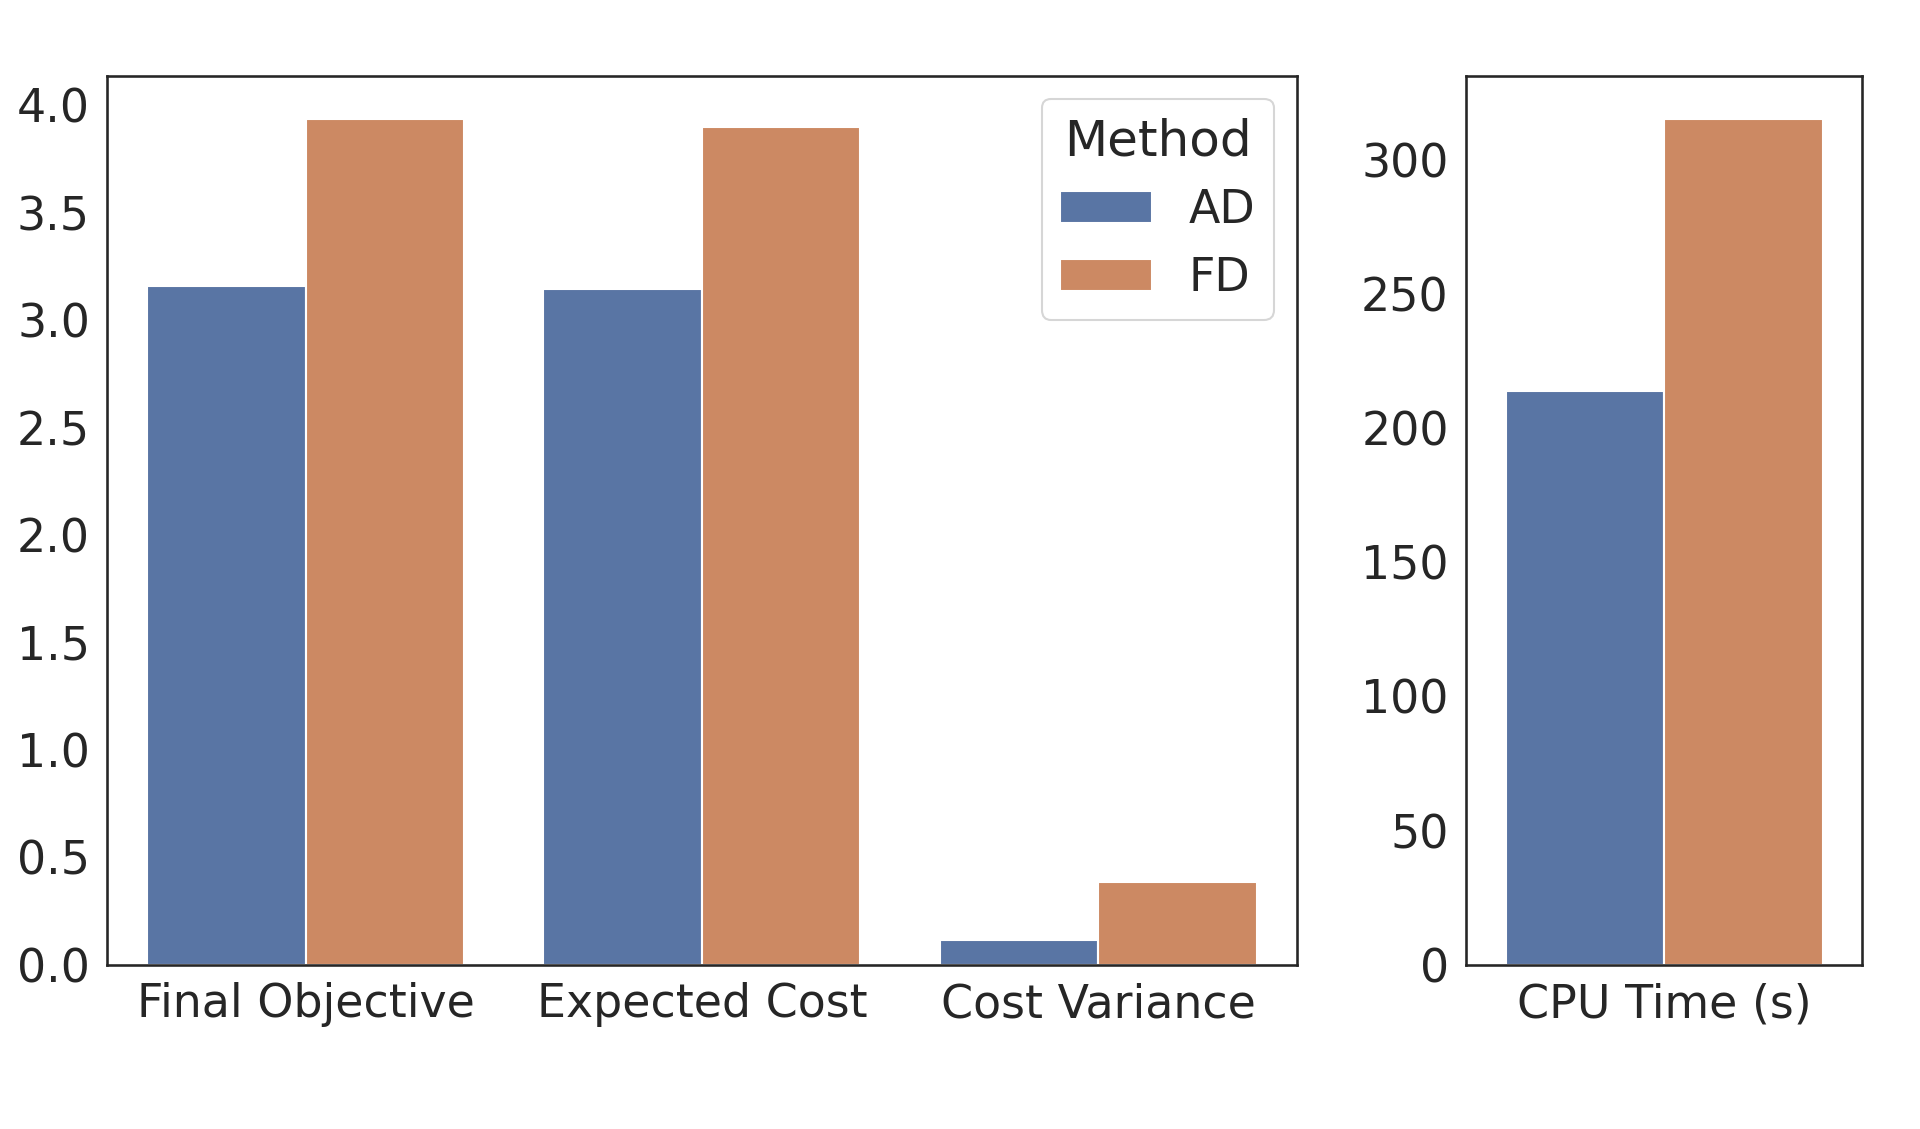
\includegraphics[width=\linewidth]{rss/agv_ad_fd_ablation.png}
        \caption{AD vs. FD; sensor placement}
    \end{subfigure}%
    % \ \\
    % \ \\
    \begin{subfigure}[t]{0.45\linewidth}
        \centering
        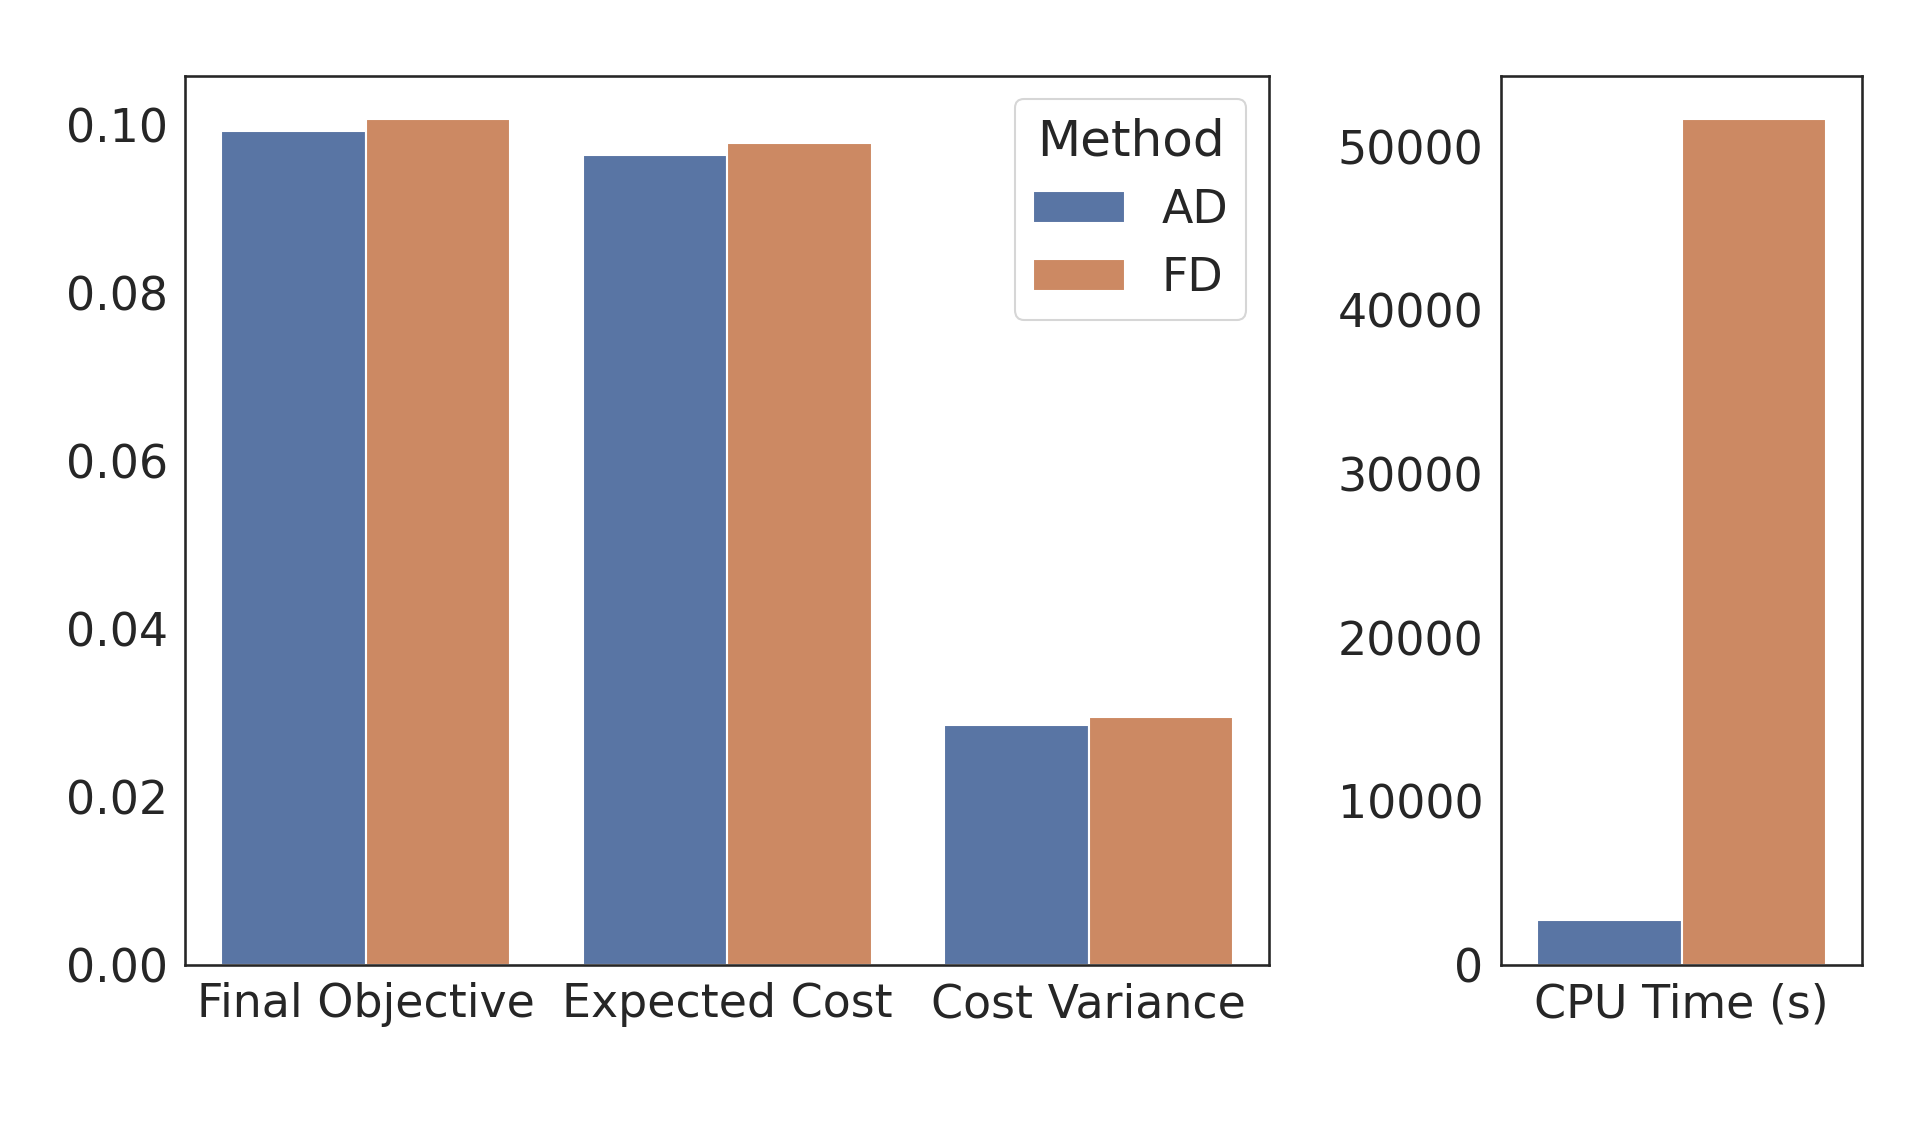
\includegraphics[width=\linewidth]{rss/mam_ablation_ad_fd.png}
        \caption{AD vs. FD; manipulation}
    \end{subfigure}
    \begin{subfigure}[t]{0.45\linewidth}
        \centering
        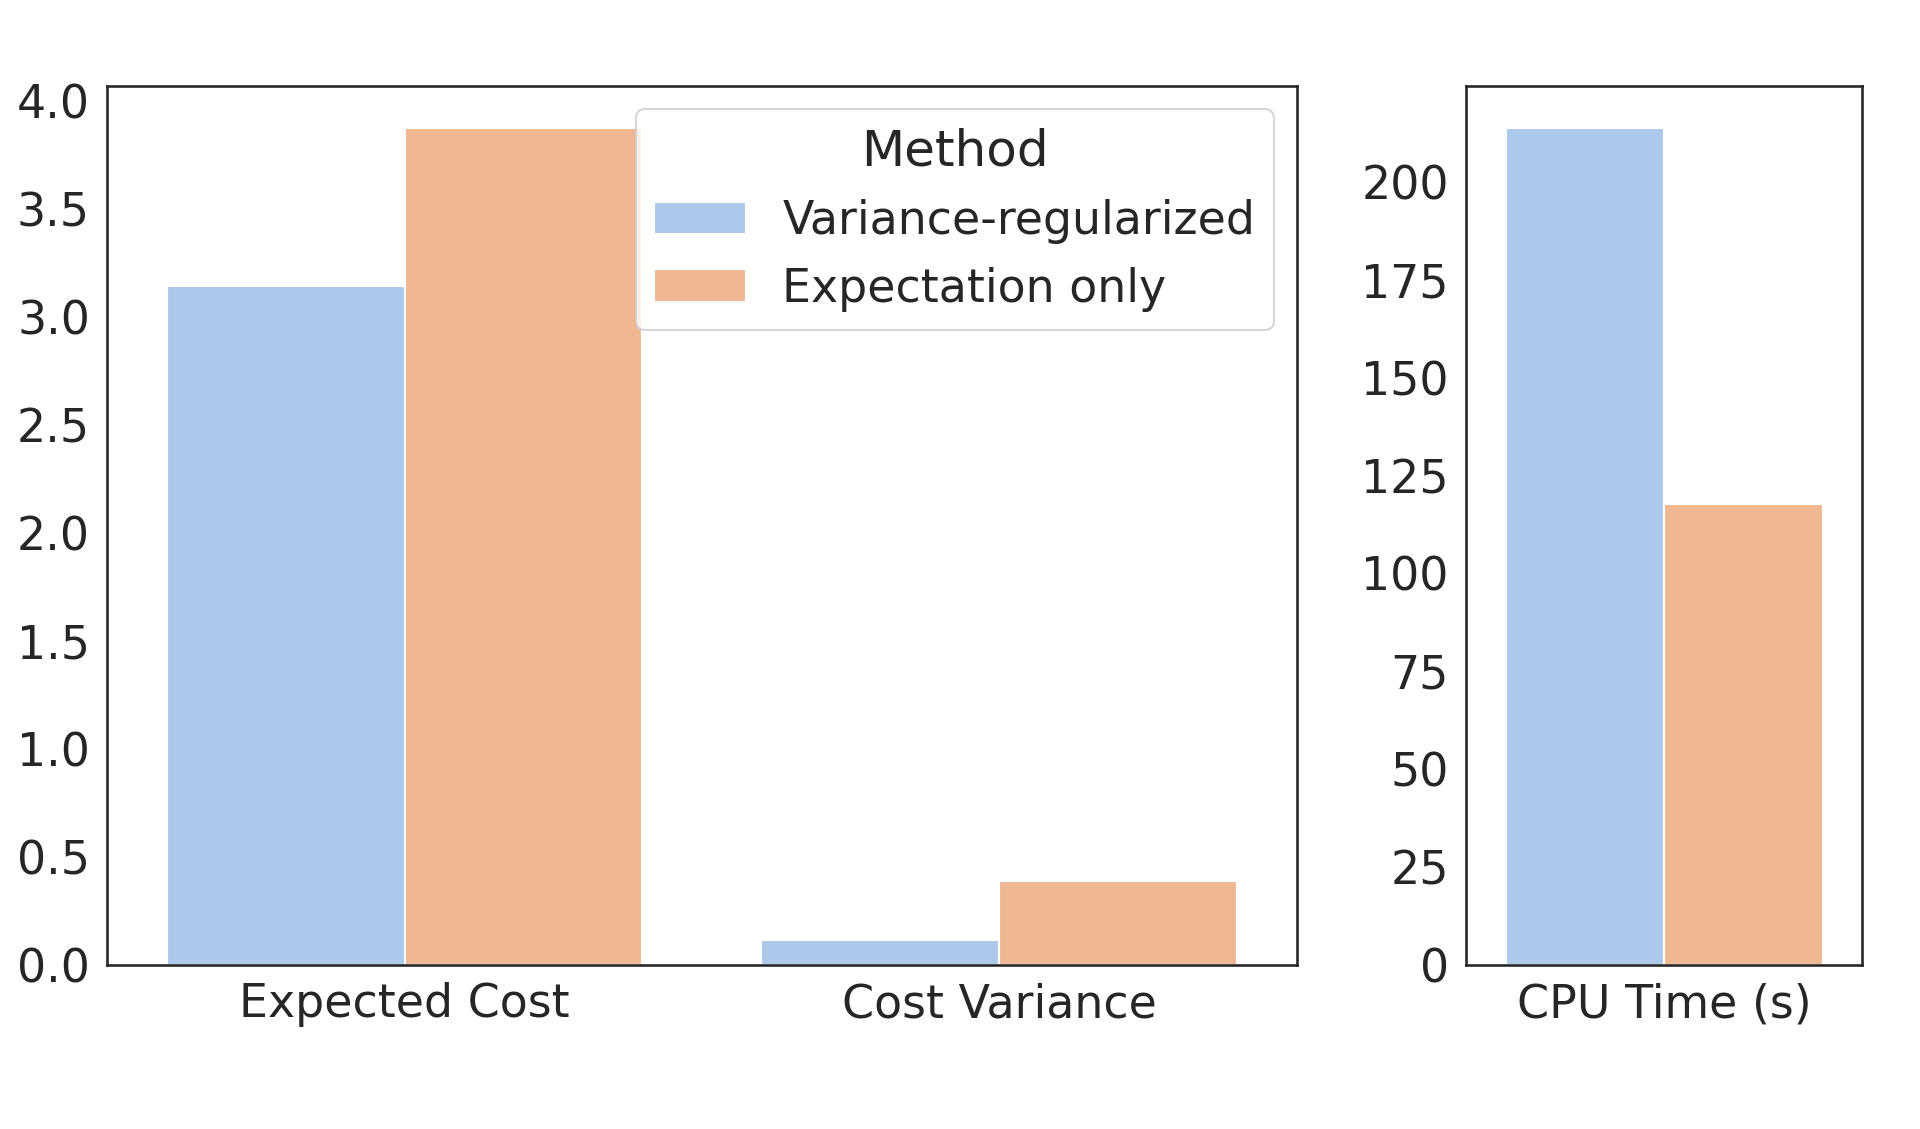
\includegraphics[width=\linewidth]{rss/agv_vr_ablation.png}
        \caption{Effect of VR; sensor placement}
    \end{subfigure}%
    % \ \\
    % \ \\
    \begin{subfigure}[t]{0.45\linewidth}
        \centering
        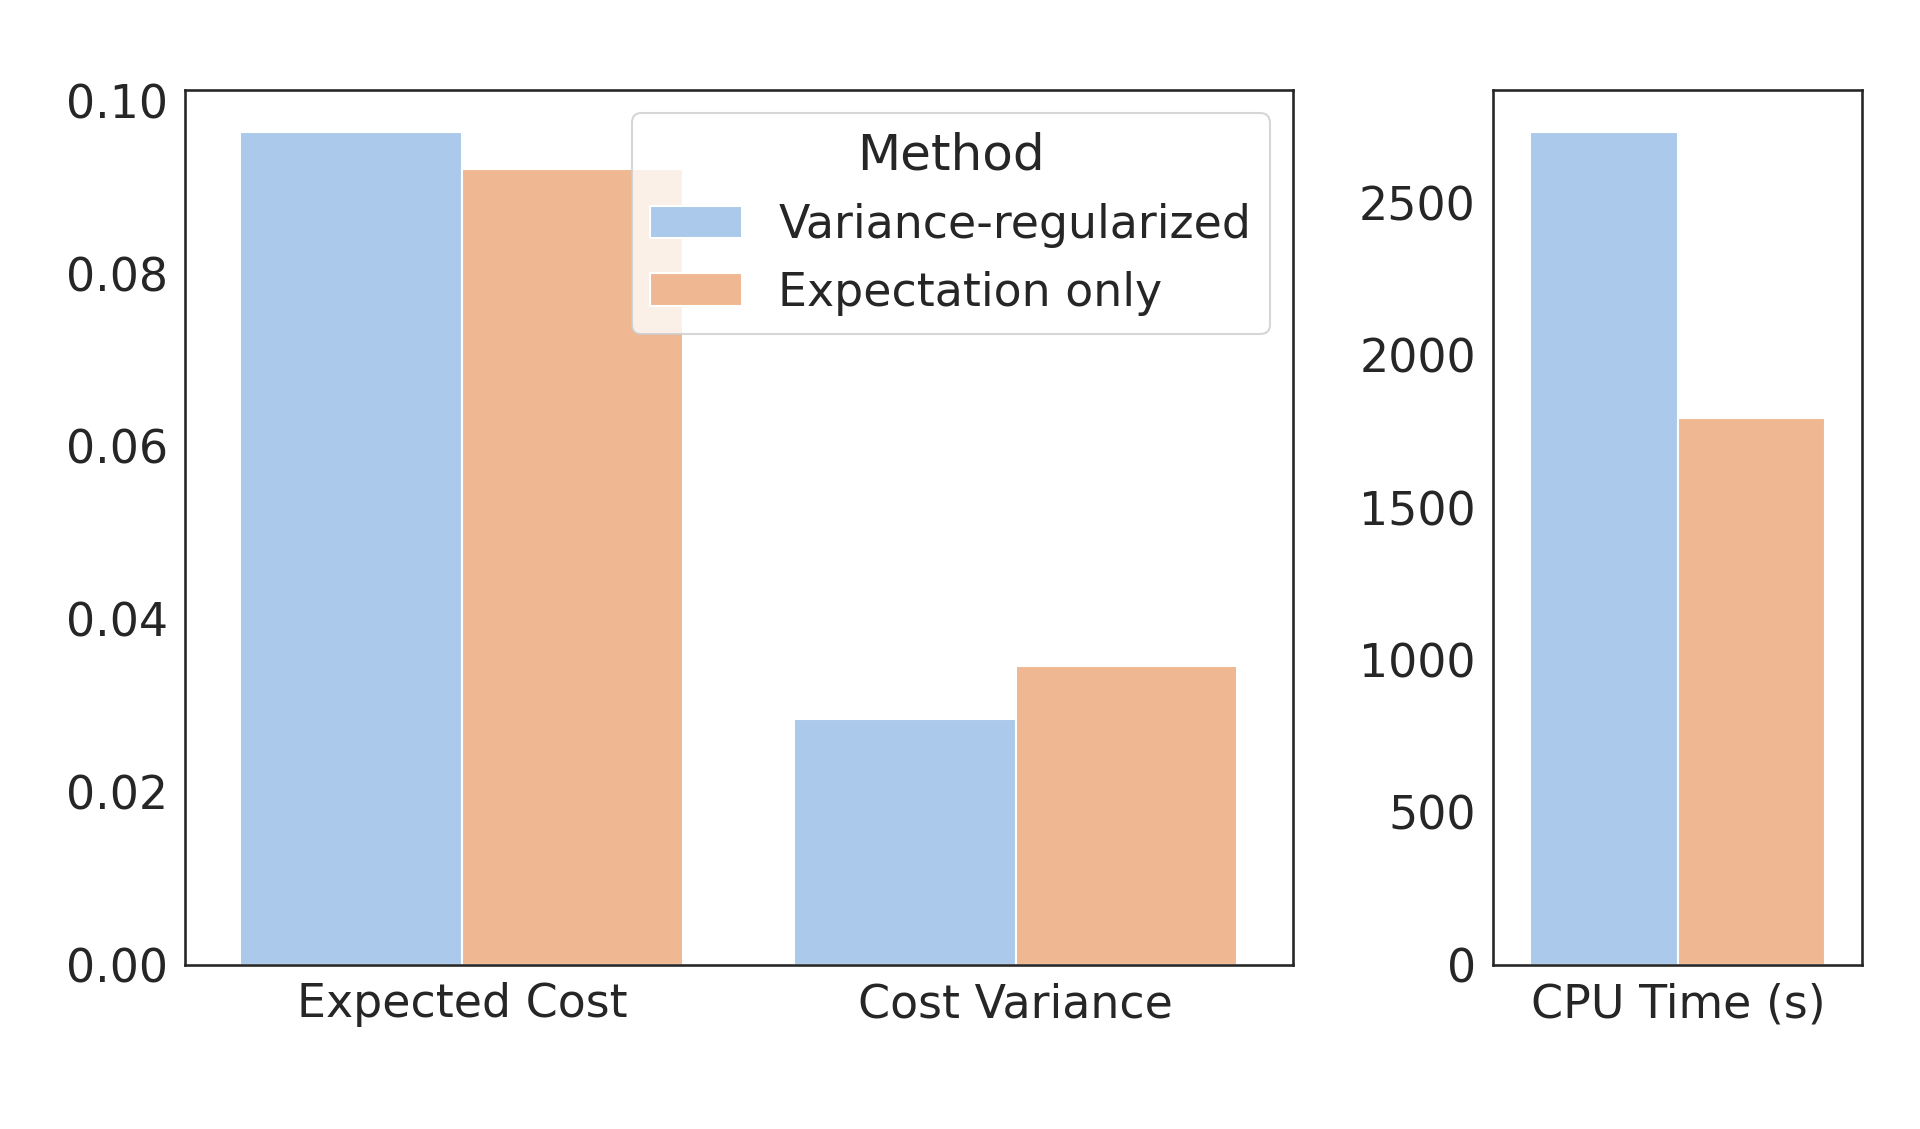
\includegraphics[width=\linewidth]{rss/mam_ablation_vr.png}
        \caption{Effect of VR; manipulation}
    \end{subfigure}
    \caption{(a)-(b) Improvement of automatic differentiation (AD) over finite differences (FD) in both case studies. (c)-(d) Effect of variance regularization (VR) in both case studies.}
    \label{ch:rss:fig:ablation}
\end{figure}

Our case studies in Sections~\ref{ch:rss:case1} and~\ref{ch:rss:case2} help demonstrate the utility of our framework for solving realistic robotics problems. However, it remains to justify the choices we made in designing this framework. For instance, how does automatic differentiation compare with other methods for estimating the gradient (e.g. finite differences)? What benefit does variance regularization in problem~\eqref{ch:rss:design_optimization_nlp} bring? We answer these questions here using an ablation study where we attempt to isolate the impact of each of these features.

First, why use automatic differentiation? On the one hand, AD allows us to estimate the gradient with only a single evaluation of the objective function, while other methods (such as finite differences, or FD) require multiple evaluations. On the other hand, AD necessarily incurs some overhead at runtime, making each AD function call more expensive than those used in an FD scheme. Additionally, some arguments~\cite{suh2021_bundled_gradients} suggest that exact gradients may be less useful than finite-difference or stochastic approximations when the objective is stiff or discontinuous. We compare AD with a 3-point finite-difference method by re-solving problem~\eqref{ch:rss:design_optimization_nlp} for both case studies, keeping all parameters constant ($N=512$, $\lambda=0.1$, same random seed) and substituting the gradients obtained using AD for those computed using finite differences. Fig.~\ref{ch:rss:fig:ablation} shows the results of this comparison. In the sensor placement example, AD achieves a lower expected cost and cost variance, and it runs in 32\% less time. In the collaborative manipulation example, both methods achieve similar expected cost and variance, but the AD version runs nearly 19x faster. These results lead us to conclude that AD enables more effective optimization than finite differences and is an appropriate choice for our framework.

The next question is whether variance regularization brings any benefit to the design optimization problem. To answer this question, we compare the results of re-solving both case studies with variance weight $\lambda = 0.1$ and $\lambda = 0$. These results are shown in Fig.~\ref{ch:rss:fig:ablation}; surprisingly, in the sensor placement example we see that the variance-regularized problem results in a lower expected cost, contrary to the intuition that regularization requires a trade off with increased expected cost. We expect that this lower expected cost may be a result of the regularization term smoothing the objective with respect to the exogenous parameters. However, these benefits are less pronounced than the benefits from automatic differentiation, and we do not see a distinct benefit from variance regularization in our second case study.

% \begin{figure}[tb]
%     \centering
%     \begin{subfigure}[t]{0.7\linewidth}
%         \centering
%         % \caption{Sensor placement}
%         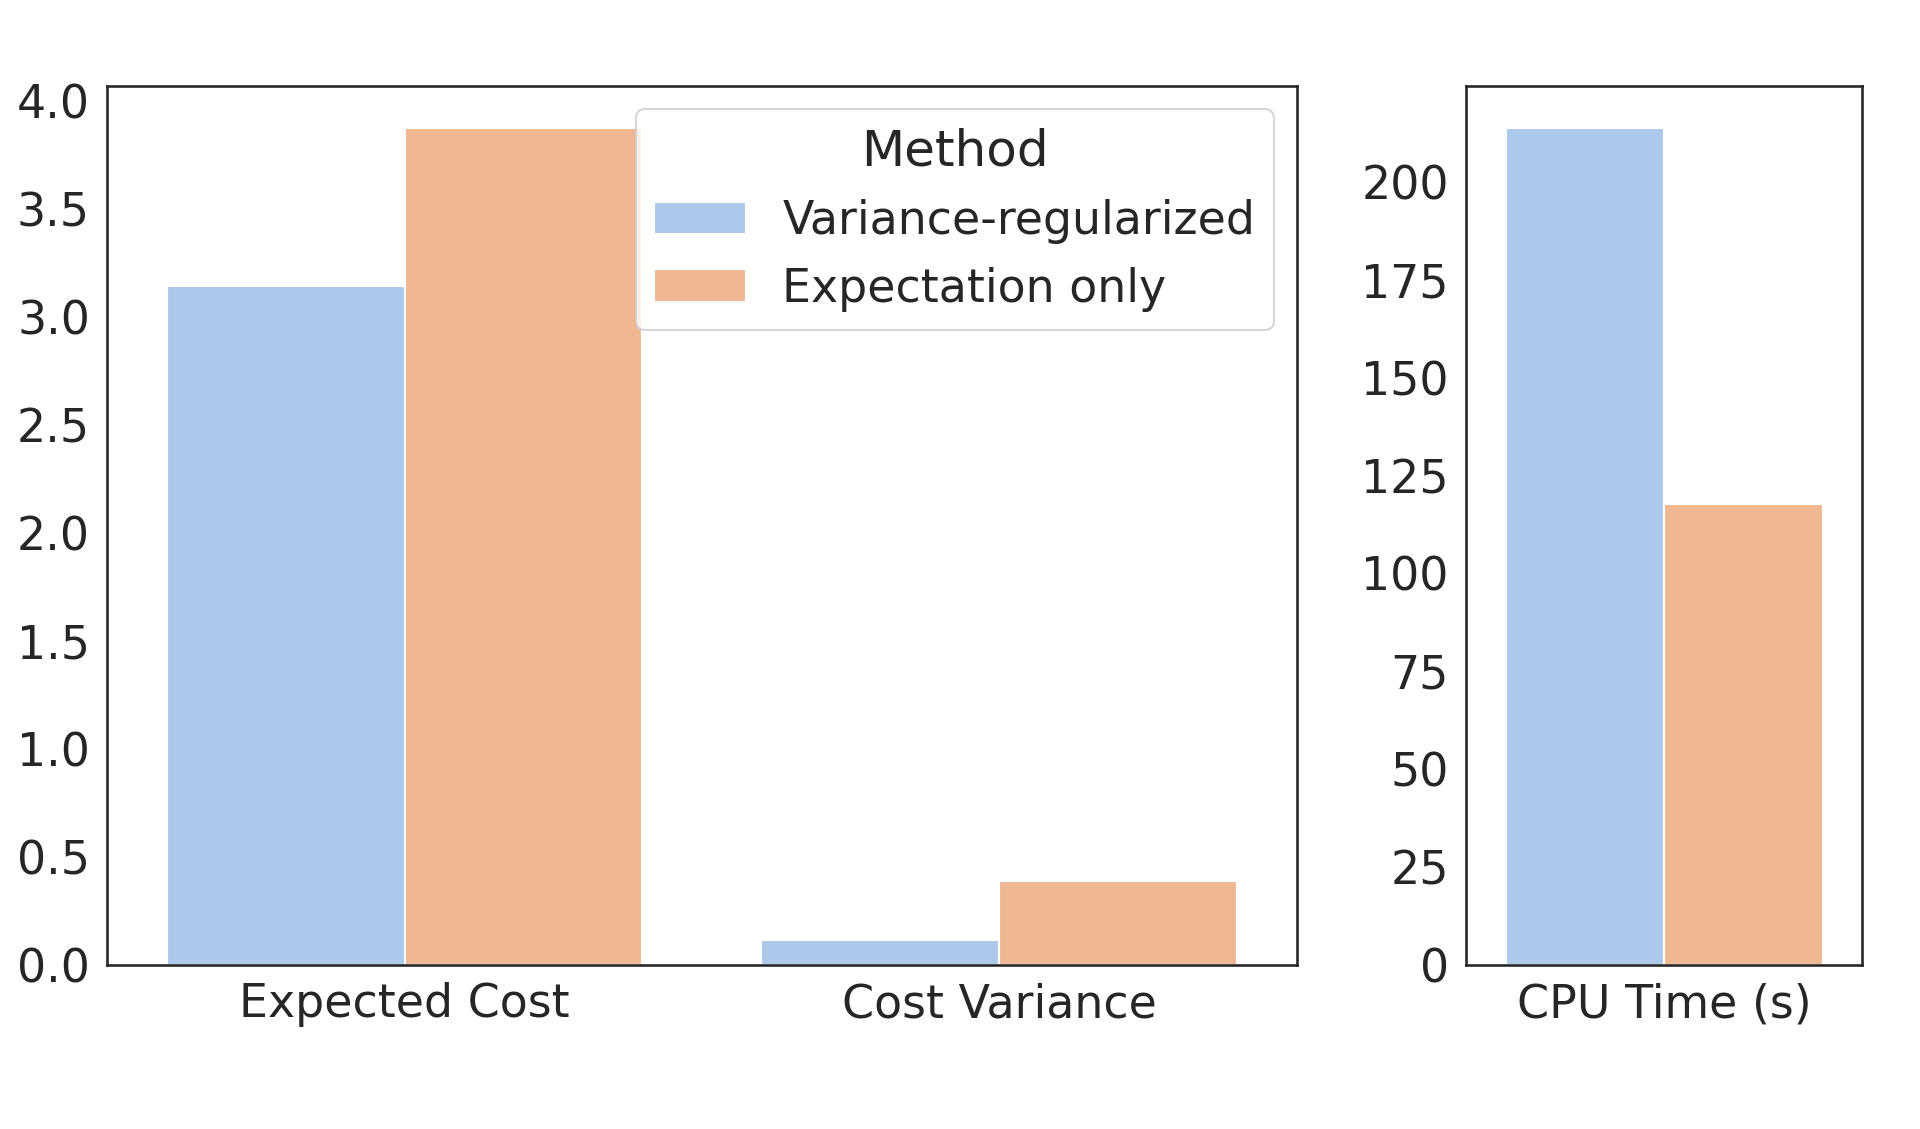
\includegraphics[width=\linewidth]{rss/agv_vr_ablation.png}
%     \end{subfigure}
%     % \ \\
%     % \ \\
%     \begin{subfigure}[t]{0.7\linewidth}
%         \centering
%         % \caption{Collaborative manipulation}
%         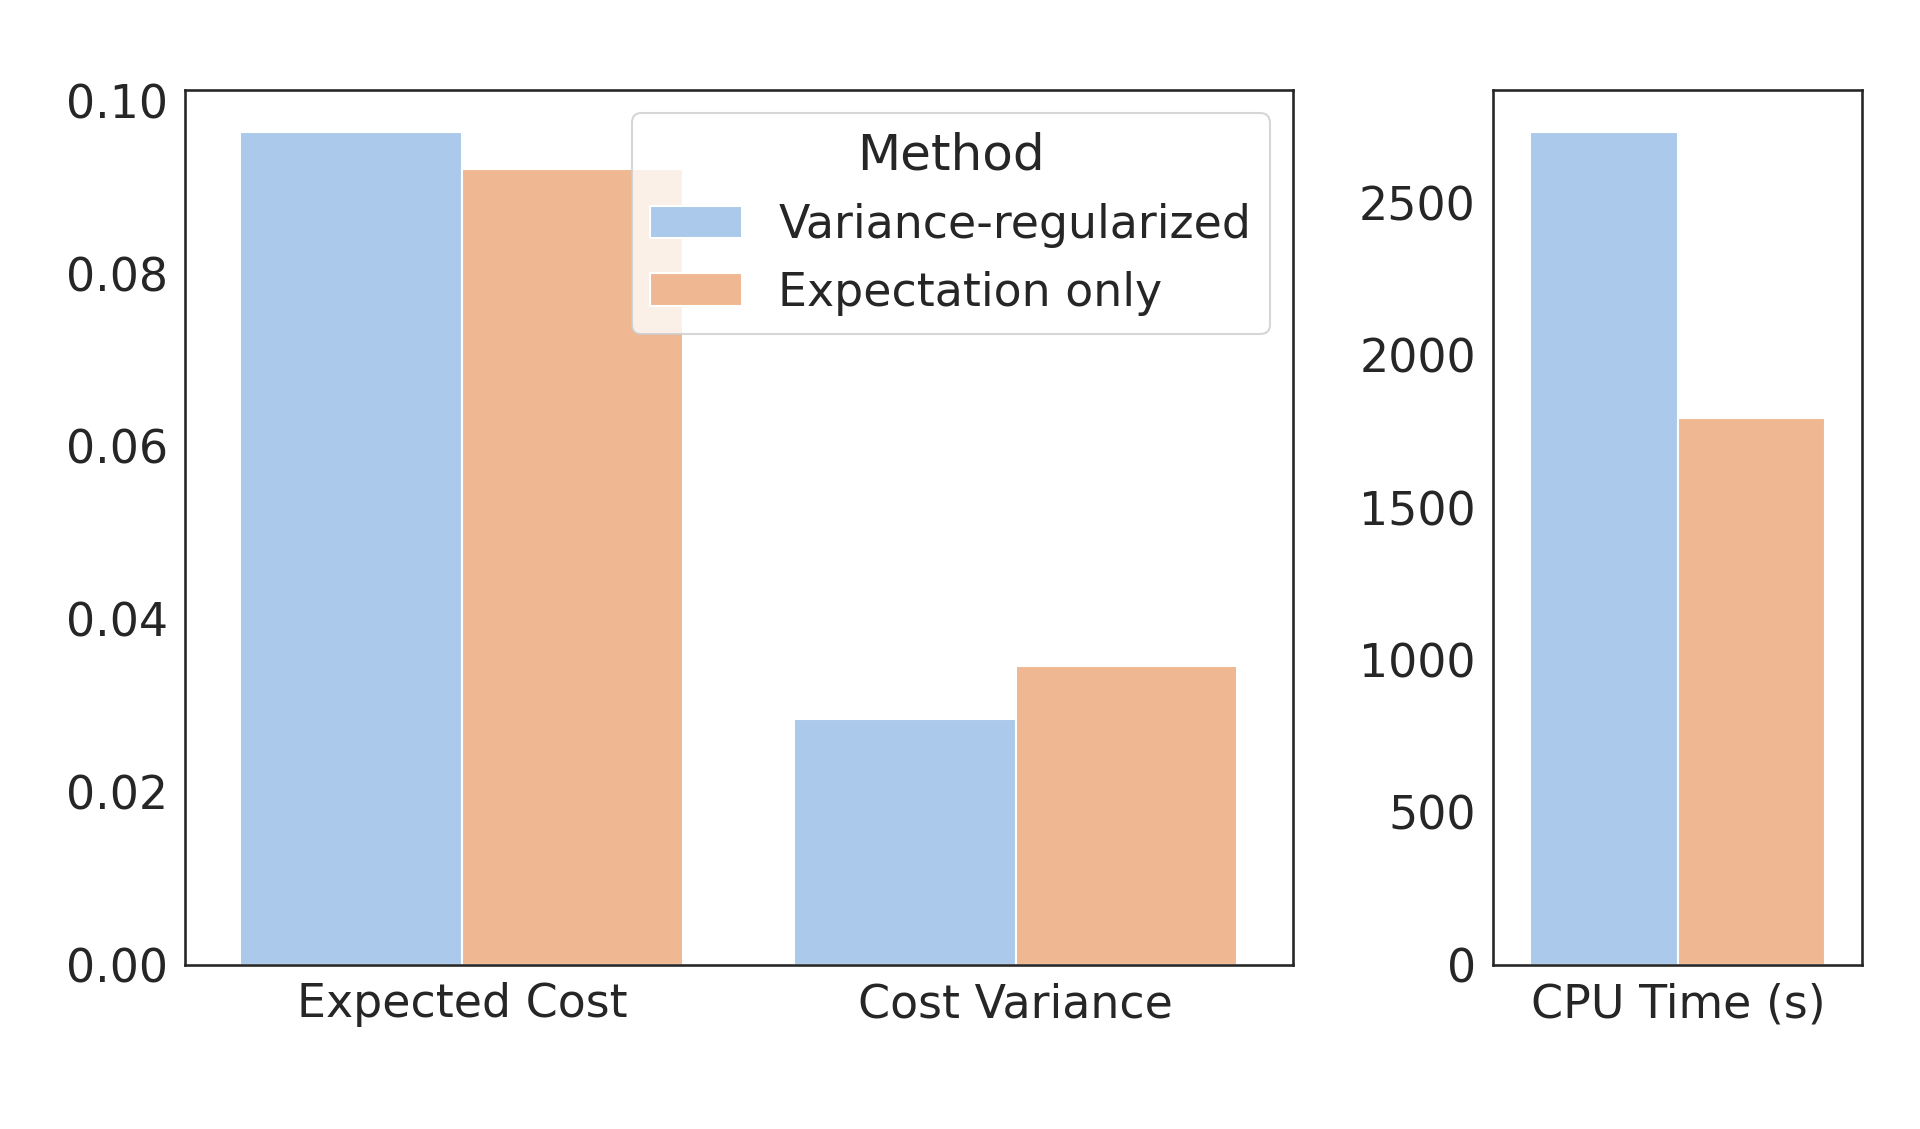
\includegraphics[width=\linewidth]{rss/mam_ablation_vr.png}
%     \end{subfigure}
%     \caption{Comparison of variance-regularized and expectation-only objectives in the sensor placement (top) and collaborative manipulation (bottom) case studies.}
%     \label{ch:rss:fig:vr_ablation}
% \end{figure}

\subsection{Accuracy of robustness analysis}\label{ch:rss:soundness}

To verify the soundness of our statistical robustness analysis methods, we need to determine whether the fit GEVD is likely to either under- or overestimate the worst-case performance of a design. To answer this question, we compare the cumulative distribution function (CDF) of the fit GEVD with an empirical CDF observed from data. Algorithms~\ref{ch:rss:alg:worst_case_cost} and~\ref{ch:rss:alg:sensitivity} both estimate a posterior distribution for $\mu$, $\sigma$, and $\xi$, allowing us to construct an upper-bound and lower-bound GEVD using the 97\% and 3\% confidence level parameter estimates. Using these distributions, we can measure false optimism and conservatism using a one-sided Kolmogorov-Smirnov (KS) test~\cite{nist_ks}.

Fig.~\ref{ch:rss:fig:ks_test} compares the estimated GEVDs and empirical data for worst-case performance in the sensor placement example (fit using Algorithm~\ref{ch:rss:alg:worst_case_cost}) and sensitivity in the manipulation example (fit using Algorithm~\ref{ch:rss:alg:sensitivity}). In the former case, we see that the empirical CDF lies between the upper- and lower-confidence limits for the fit distribution, indicating that the fit is neither falsely optimistic at the 97\% level nor conservative at the 3\% level (these conclusions are confirmed by the KS statistics provided in Table~\ref{ch:rss:tab:ks_test_agv}). In the second case study, even though the empirical CDF extends slightly beyond the estimated bounds in some regions, the statistical analysis in Table~\ref{ch:rss:tab:ks_test_mam} indicates that the estimated GEVD is neither falsely optimistic at the 97\% level nor conservative at the 3\% level. In addition, we see that the gap between the 3\% and 97\% distributions is relatively small in both examples in Fig.~\ref{ch:rss:fig:ks_test}.

\begin{figure}[tb]
    \centering
    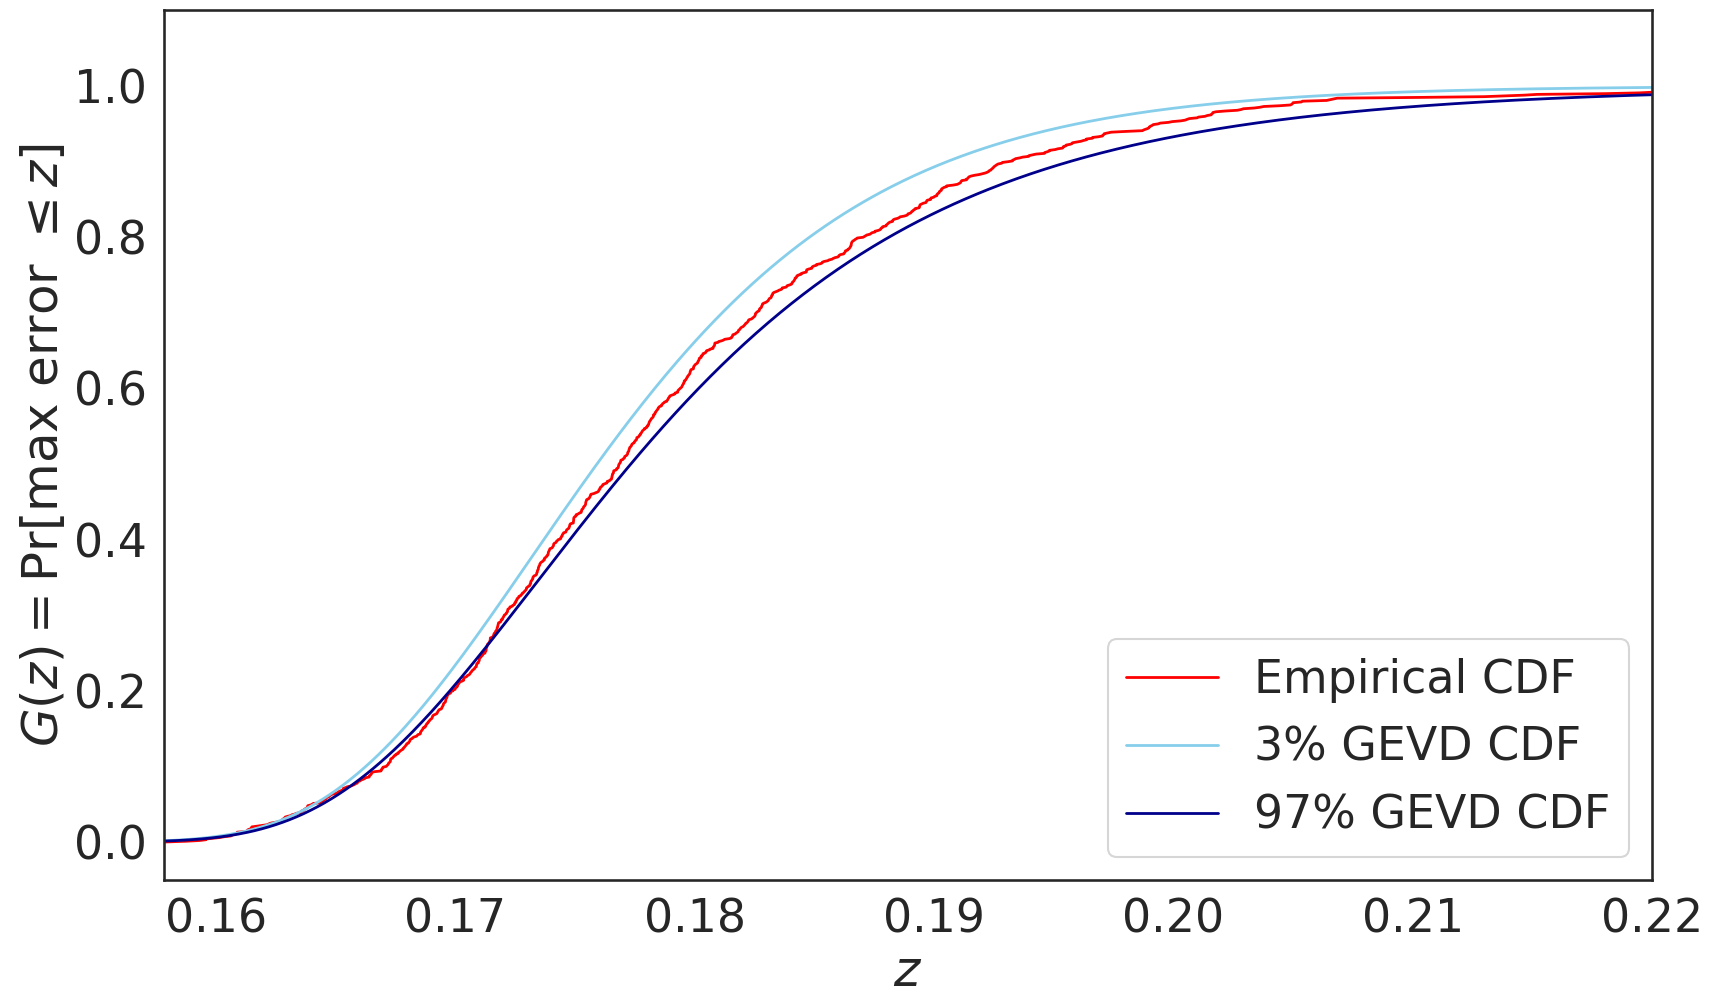
\includegraphics[width=0.45\linewidth]{rss/agv_gevd_comp.png}
    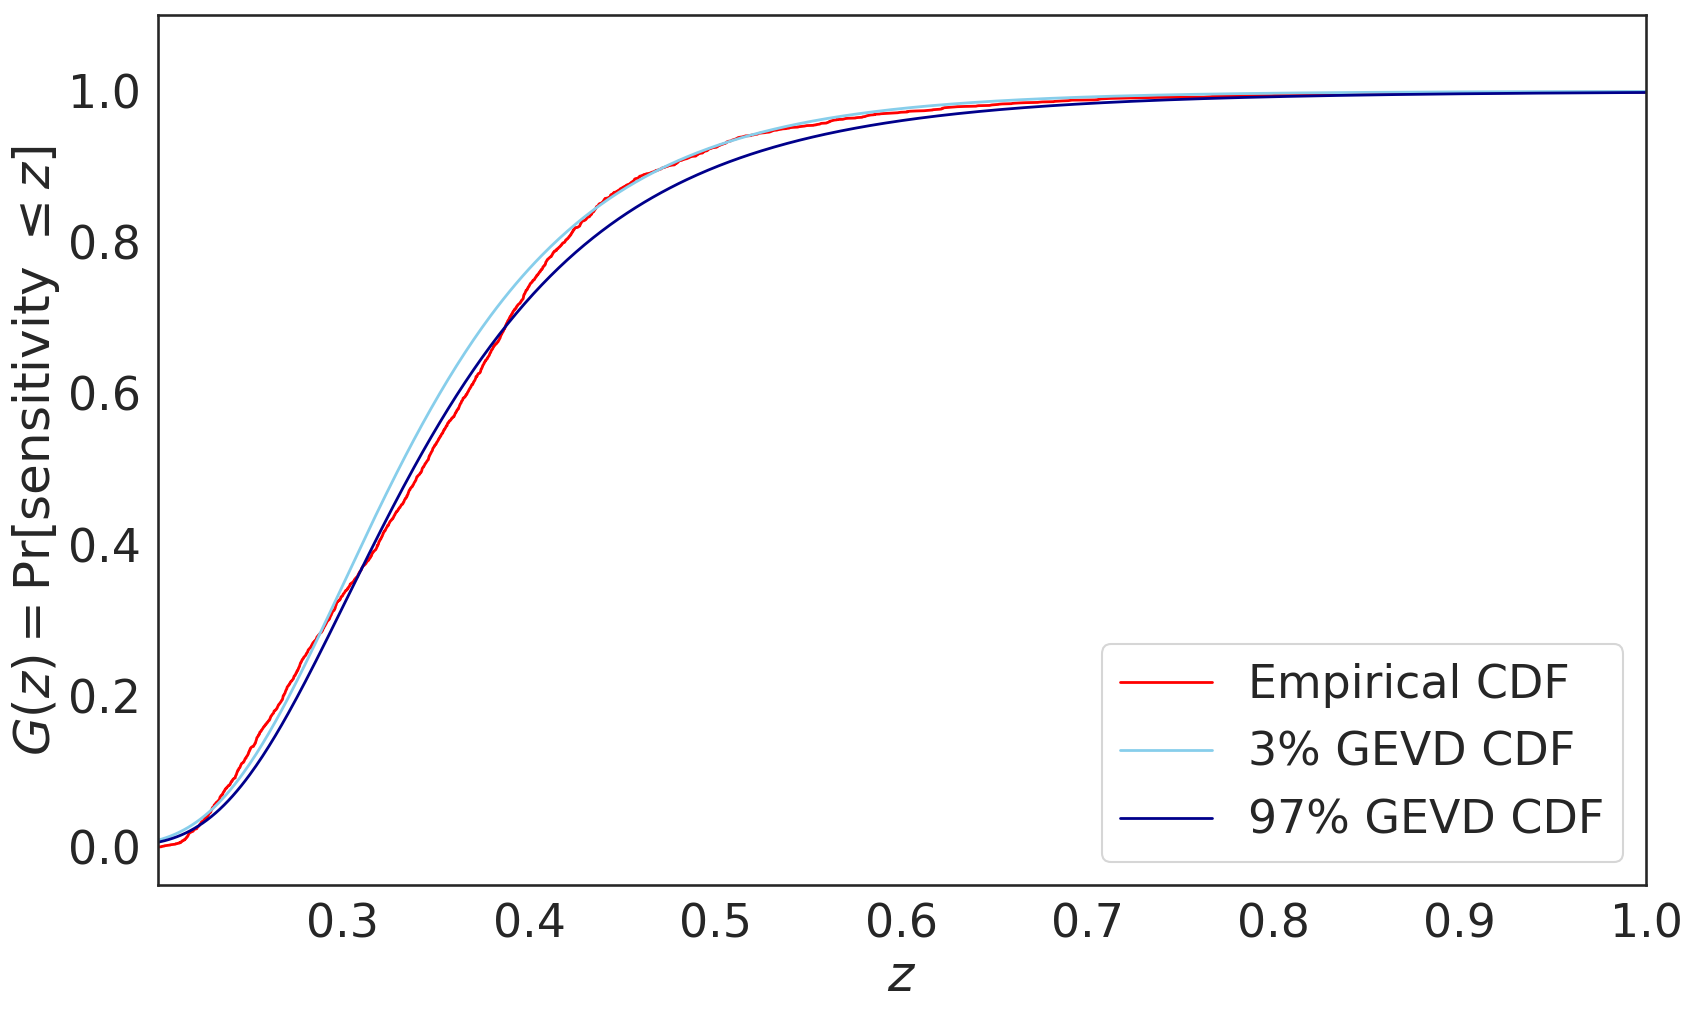
\includegraphics[width=0.45\linewidth]{rss/mam_gevd_comp_friction.png}
    \caption{Comparison of fit GEVD CDFs and empirical CDF for worst-case estimation error in the sensor placement example (top) and sensitivity in the manipulation example (bottom).}
    \label{ch:rss:fig:ks_test}
\end{figure}


\begin{table}[thb]
    \renewcommand{\arraystretch}{1.5}
    \centering
    \begin{tabular}{r||p{4cm}|c|c|p{5cm}}
                       & Null Hypothesis                                  & \shortstack{KS                                                                                       \\ Statistic} & p-value & Conclusion ($p < 0.05$)                                                   \\ \hline\hline
        False Optimism & 97\% GEVD under-estimates worst-case performance & 0.0410         & 0.0337  & Reject; 97\% GEVD \textit{does not} under-estimate worst-case performance \\ \hline
        Conservatism   & 3\% GEVD over-estimates worst-case performance   & 0.0529         & 0.00354 & Reject; 3\% GEVD \textit{does not} over-estimate worst-case performance
    \end{tabular}
    \caption{Results of one-sided KS tests for the sensor placement case study. These results indicate that Algorithm~\ref{ch:rss:alg:worst_case_cost} is sound in this case.}\label{ch:rss:tab:ks_test_agv}
\end{table}

\begin{table}[thb]
    \renewcommand{\arraystretch}{1.5}
    \centering
    \begin{tabular}{r||p{4cm}|c|c|p{5cm}}
                       & Null Hypothesis                       & \shortstack{KS                                                                                         \\ Statistic} & p-value              & Conclusion ($p < 0.05$)                                        \\ \hline\hline
        False Optimism & 97\% GEVD under-estimates sensitivity & 0.0399         & $6.75\times10^{-5}$  & Reject; 97\% GEVD \textit{does not} under-estimate sensitivity \\ \hline
        Conservatism   & 3\% GEVD over-estimates sensitivity   & 0.0618         & $1.03\times10^{-10}$ & Reject; 3\% GEVD \textit{does not} over-estimate sensitivity
    \end{tabular}
    \caption{Results of one-sided KS tests for the collaborative manipulation case study. These results indicate that Algorithm~\ref{ch:rss:alg:sensitivity} is sound in this case.}\label{ch:rss:tab:ks_test_mam}
\end{table}

\section{Summary}

In this chapter, we introduce an automated design tool to improve the productivity of robot designers by a) enabling efficient optimization of robot designs and b) allowing users to certify the robustness of those designs. In developing this framework, we make two main contributions. First, we use differentiable programming for end-to-end optimization of robotic systems, creating a flexible software framework for design optimization. Second, we develop a novel statistical framework for certifying the worst-case performance and sensitivity of optimized designs.
%
We apply these tools to optimize the design of two robotic systems in hardware. We use our statistical certification method to test the robustness of these designs, and we show that the optimized designs are robust enough to deploy in hardware. We hope that by combining flexible design optimization with robustness certification, this framework makes the first steps towards developing the automated design aid for robotics engineers envisioned by this thesis.

That said, there are several limitations with the approach presented in this chapter. First, since our approach relies on sampling from $\Phi$ without any further information, it will require a large number of samples to accurately capture rare events. As we will see in the following chapters, we can close this gap when more information about $\Phi$ is available by using adversarial optimization and Bayesian inference techniques. Second, the statistical verification method yields an estimate of the worst-case cost, but it does not provide any insights into what environmental factors could lead to that worst-case performance. Finally, the optimization approach presented in this chapter is based on gradient descent, which is inherently local (i.e. it risks converging to a suboptimal solution) and prone to failing when the gradients of $J\circ S$ are not well behaved. We will address both of these limitations in the following chapters, starting with an adversarial optimization method that reduces the number of samples from $\Phi$ required for robust solutions, and then discussing a novel reformulation of the end-to-end design optimization problem that allows us to search for (approximately) globally optimal solutions and avoid issues due to poorly conditioned gradients.
% This chapter is based on my IROS paper, for which IEEE holds the copyright.
\newcommand{\ieeecopyright}{\copyright 2022 IEEE}

\chapter{Counterexample-guided Optimization with Formal Specifications}\label{ch:iros}

In the previous chapter, we saw how automatic differentiation can enable end-to-end design optimization for a range of robotic systems. However, the optimization algorithm presented in Chapter~\ref{ch:rss} relies on a variance-regularization heuristic to encourage the robustness of the optimized designs. There are two issues with this approach, which we address in this chapter. First, estimating the cost variance requires a large number of samples of the exogenous parameters $\phi$. Second, the methods presented in Chapter~\ref{ch:rss} provide a statistical estimate of the worst-case cost, but they do not provide concrete counterexamples; i.e., specific values of $\phi$ that lead to high cost.

In this chapter, we address both of these issues through the development of a \textit{counterexample-guided} design optimization pipeline that replaces the variance regularization used in Chapter~\ref{ch:rss} with an adversarial optimization procedure that alternates between optimizing the design $\theta$ and a set of adversarial counterexamples $\phi$. In addition, we use differentiable temporal logic to allow users to formally specify the desired behavior of the robot. This chapter is based on the author's published work~\cite{dawsonRobustCounterexampleguidedOptimization2022b}.

There are different types of temporal logic that may be used to specify robot behaviors, but here we focus on \textit{signal temporal logic} (STL), a formal language for specifying properties of real-values continuous-time signals~\cite{donzeBreachToolboxVerification2010,sunMultiagentMotionPlanning2022,pantSmoothOperatorControl2017}. Using STL, users can specify a variety of robot behaviors by combining logical and temporal operators to specify the desired order and dependencies between subtasks~\cite{plakuMotionPlanningTemporallogic2016,sunMultiagentMotionPlanning2022,takanoContinuousOptimizationBasedTask2021}. Although the syntax of STL can be opaque, there are tools for translating between STL and natural language~\cite{chenNL2TLTransformingNatural2023}.

A number of previous works have approached the problem of synthesizing robot behaviors from STL specifications, using either abstraction-based methods~\cite{plakuMotionPlanningTemporallogic2016}, mixed-integer optimization~\cite{sunMultiagentMotionPlanning2022,yangSynthesisguidedAdversarialScenario2021}, sampling-based planning~\cite{kantaros20,vasile17}, or nonlinear optimization~\cite{pantFlybyLogicControlMultiDrone2018,pantazidesSatelliteMissionPlanning2022,leungBackPropagationSignalTemporal2021}.
%
Abstraction-based methods first discretize the state space, then plan on this discrete domain; these methods have a long history but suffer from exponential dependence on problem dimension. Mixed-integer optimization-based methods encode the STL specification as linear constraints with integer variables, resulting in soundness and completeness guarantees, but the resulting mixed integer programs (MIPs) become intractable for problems with a large state space or long task horizon~\cite{sadraddiniRobustTemporalLogic2016,yangSynthesisguidedAdversarialScenario2021,raman15}. The size of the MIP can be reduced using a timed waypoint representation, but this requires restrictive assumptions (e.g. access to a tracking controller with bounded error~\cite{sunMultiagentMotionPlanning2022}).

Some recent work uses nonlinear optimization to solve robot planning problems with STL specifications~\cite{pantSmoothOperatorControl2017,pantazidesSatelliteMissionPlanning2022,leungBackPropagationSignalTemporal2021,takanoContinuousOptimizationBasedTask2021,leeSignalTemporalLogic2021}. These methods achieve improved scalability through the use of smooth approximations of STL and local gradient-based optimization methods, but they sacrifice completeness and optimality guarantees and can result in solutions with poor robustness (as we demonstrate via our experiments later in this section).

The primary gap in the state-of-the-art for robot optimization with STL constraints is that existing methods do not explicitly consider robustness to environmental uncertainty or disturbances (\cite{leeSignalTemporalLogic2021} considers probability of satisfaction, but not robustness to worst-case uncertainty). Existing methods implicitly encourage robustness by maximizing the margin by which the STL specification is satisfied, but in practice we find that this is not sufficient to prevent failure when confronted with environmental uncertainty. Some methods do explicitly consider worst-case robustness~\cite{raman15}, but our experiments indicate that these methods yield MIPs that are too computationally expensive to solve in practice.

In this chapter, we address this gap by extending the end-to-end optimization method presented in Chapter~\ref{ch:rss} to use counterexamples (i.e. a set of adversarially-chosen environmental parameters $\phi$) to guide the optimization of the design parameters $\theta$. This method uses an iterative adversarial optimization scheme inspired by solution methods for multi-player games, alternating between searching for a design that performs well against a set of known counterexamples and searching for new counterexamples to guide the design process. This approach relies on differentiable simulation, as discussed in Chapter~\ref{ch:rss}, with the addition of differentiable temporal logic for formal task specifications.

This chapter is organized as follows: after briefly reviewing the syntax and semantics of STL, we extend the problem statement from Chapter~\ref{ch:rss} to include STL specifications. We then present our approach to counterexample-guided optimization, and conclude with numerical experiments that demonstrate the improved performance of our method relative to state-of-the-art mixed-integer and nonlinear optimization methods. We find that our approach not only yields designs that satisfy the STL specification despite worst-case environmental uncertainty, but also that it requires less than half of the optimization time as the next-most-successful method. Our counterexample-guided method scales to handle long-horizon tasks that are not tractable for MIP-based methods, and the designs found using our approach are consistently more robust than those generated by competing methods.

\section{Background on signal temporal logic}

Recall from Chapter~\ref{ch:rss} that we described the behavior of the system by the discrete trace of states over a fixed horizon $T$: $s_1, \ldots, s_T$. In this chapter, we extend this view by considering behaviors in continuous time $s(t)$, which for convenience we represent as piecewise-linear interpolation between timed samples $(t_i, s_i)$. Moving from a discrete sequence of states to a piecewise-linear continuous signal allows us to be more precise in specifying the desired robot behavior, since we can now be explicit about the state of the robot in between sampled times while maintaining a finite-dimensional representation.

Given this representation, we can specify the desired behavior of a robot using signal temporal logic (STL). STL is a formal language for specifying how a signal should evolve over time, and it allows us to express complex requirements for how a robot behaves over time. The rest of this section will cover formal STL syntax (how requirements are written) and semantics (how they are interpreted).

\subsection{Syntax of signal temporal logic}

STL requirements are expressed as \textit{formulas}, which can be build out of three basic building blocks: predicates, logical operators, and temporal operators. Predicates are functions that map a continuous-time signal to a Boolean value, and they can be used to express properties of the robot's state or the environment (e.g. is a robot in a given state at a given time). Logical operators are used to combine predicates, and temporal operators are used to express how predicates should evolve over time~\cite{donzeEfficientRobustMonitoring2013a}. We can define the syntax of an STL formula $\psi$ recursively as:
\begin{align}
	\psi = \text{true}\ |\ \mu(x) \geq 0\ |\ \neg \psi\ |\ \psi_1 \wedge \psi_2\ |\ \psi_1 \ \until_I\ \psi_2\label{ch:iros:stl_syntax}
\end{align}
with closed (but potentially unbounded) time interval $I$, predicate $\mu: \mathcal{S} \rightarrow \R$ mapping states to real numbers, logical operators $\neg$ (negation) and $\wedge$ (conjunction), and temporal operator ``until'' $\until_I$, which can be read as ``within interval $I$, $\psi_1$ must be true until $\psi_2$ becomes true''. For convenience, we assume $I = [0, \infty)$ when not explicitly specified. Additional temporal operators can be defined in terms of these basic building blocks:
\begin{enumerate}
	\item Eventually: $\eventually_I\ \psi = \text{true } \until_I\ \psi$; read as ``$\psi$ must be true at least once during $I$''.
	\item Always: $\always_I = \neg \eventually_I\ \neg \psi$; read as ``$\psi$ must be true at all times during $I$''.
\end{enumerate}
Similarly, the usual suite of logical operators (e.g. or, implies) can be defined in terms of the basic logical operators. The syntax of STL can be opaque for unfamiliar readers; wherever possible in this thesis, STL specifications will be accompanied by natural language explanations.

\subsection{Semantics of signal temporal logic}

There are two related ways of interpreting any given STL formula: the Boolean and quantitative semantics. Given an STL formula $\psi$, the Boolean semantics assign a simple true/false value to a signal $s$ at a particular time $t$ indicating whether the STL formula is satisfied at that time~\cite{donzeEfficientRobustMonitoring2013a}:
\begin{alignat*}{3}
	 & s, t &  & \models \text{true}              &  &                                                                            \\
	 & s, t &  & \models \mu(x) \geq 0\quad       &  & \text{iff}\ \mu(s(t)) \geq 0                                               \\
	 & s, t &  & \models \neg \psi                &  & \text{iff}\ s, t \not\models \psi                                          \\
	 & s, t &  & \models \psi_1 \wedge \psi_2     &  & \text{iff}\ s, t \models \psi_1 \text{ and } s, t \models \psi_2           \\
	 & s, t &  & \models \psi_1\ \until_I\ \psi_2 &  & \text{iff } \exists\ t' \in t + I \text{ s.t. } w, t' \models \psi_2       \\
	 &      &  &                                  &  & \phantom{iff} \text{ and } w, t'' \models \psi_1\ \forall\ t'' \in [t, t']
\end{alignat*}

A useful feature of STL is that it also admits a so-called \textit{quantitative semantics}. Intuitively, if the Boolean semantics tell us whether an STL formula is satisfied by a given signal at a given time, the quantitative semantics tell us how well the signal satisfies the formula (i.e. by how much does it exceed the specified requirements, or by how much does it fall short). We denote the quantitative semantics as $\rho \maps \Psi \times \mathcal{S} \times \R^+ \rightarrow \R$, where $\rho(\psi, s, t)$ is the \textit{robustness} of the signal $s$ with respect to the formula $\psi$ at time $t$. The robustness is a real number that quantifies how well the signal satisfies the formula at that time; the formula is satisfied precisely when $\rho \geq 0$. The robustness function is defined recursively as:
\begin{align*}
	\rho(\text{true}, s, t)             & = \top                                                                                             \\
	\rho(\mu(x) \geq 0, s, t)           & = \mu(s(t))                                                                                        \\
	\rho(\neg\psi, s, t)                & = -\rho(\psi, s, t)                                                                                \\
	\rho(\psi_1 \wedge \psi_2, s, t)    & = \min\{\rho(\psi_1, s, t), \rho(\psi_2, s, t)\}                                                   \\
	\rho(\psi_1 \until_I\ \psi_2, s, t) & = \sup_{t_1 \in t + I} \min\{\rho(\psi_2, s, t_1),  \inf_{t_2 \in [t, t_1]} \rho(\psi_1, s, t_2)\}
\end{align*}
where $\top$ is a constant defined to be greater than all other real values. In practice, linear-time algorithms exist to compute $\rho$ from a given piecewise-affine signal $s$~\cite{donzeEfficientRobustMonitoring2013a}.

\section{Problem statement}

In this chapter, we extend the design optimization problem~\eqref{ch:rss:design_optimization_nlp} from Chapter~\ref{ch:rss} in two ways: first, we incorporate STL into the cost function to specify the desired robot behavior. Second, we replace the variance regularization in~\eqref{ch:rss:design_optimization_objective} with a robust adversarial formulation, which we will solve using counterexample-guided optimization. These two changes yield the robust design problem:
%
\begin{subequations}\label{ch:iros:robust_nlp_generic}
	\begin{align}
		\min_\theta\ \max_\phi & \quad \lambda J(\theta, \phi) - \rho\pn{\psi, S(\theta, \phi), 0}  \label{ch:iros:robust_objective_generic}          \\
		\text{s.t.}            & \quad c_{\theta, i}(\theta) \geq 0 \quad \forall i \in \mathcal{I}_{\theta} \label{ch:iros:robust_constraints_theta} \\
		                       & \quad c_{\phi, i}(\phi) \geq 0 \quad \forall i \in \mathcal{I}_{\phi} \label{ch:iros:robust_constraints_phi}
	\end{align}
\end{subequations}
%
where $\rho\pn{\psi, S(\theta, \phi), 0}$ is the robustness margin at the starting time $t=0$ of the system trace simulated with parameters $\theta$ and $\phi$ with respect to STL specification $\psi$. We subtract $\rho$ from a generic cost function $J$ (weighted by $\lambda > 0$) to balance maximizing STL robustness against minimizing other costs (e.g. fuel use). The scaling factor $\lambda$ is typically small to prioritize satisfying the STL specification. For convenience, we denote
\begin{equation}
	J_\psi(\theta, \phi) = J(\theta, \phi) - \rho\pn{\psi, S(\theta, \phi)}.
\end{equation}

In this adversarial formulation, we also include additional constraints~\eqref{ch:iros:robust_constraints_phi} to restrict the values of the exogenous parameters; often, unbounded exogenous parameters can lead to unbounded cost (e.g. large external disturbances that cause a robot to deviate arbitrarily far from a planned path), so bounding the exogenous parameters helps with the stability of this adversarial optimization problem.

\section{Approach}

Problem~\eqref{ch:iros:robust_nlp_generic} is a nonlinear optimization that cannot generally be solved to global optimality. Instead, we take advantage of the two-player game structure of this problem to design an iterative algorithm to find a local \textit{generalized Nash equilibrium}; i.e., the design parameters $\theta$ and corresponding adversarial exogenous parameters $\phi$ such that neither the designer nor the adversary have an incentive to change~\cite{facchineiGeneralizedNashEquilibrium2007}.

In order to solve this problem, we must address two challenges. First, in order to efficiently solve this nonlinear optimization problem, we must be able to compute gradients of $\rho$ with respect to $\theta$ and $\phi$; we address this problem using differentiable programming, as discussed in Section~\ref{ch:iros:diffstl}. Second, although gradient-based optimization is a sample-efficient method for solving problems like~\eqref{ch:iros:robust_nlp_generic}, there is a risk that the resulting local Nash equilibrium will not be robust; i.e., overfitting the design $\theta$ to a particular adversarial $\phi$ so that the design performs poorly when $\phi$ changes. We address this problem by developing a meta-heuristic for counterexample-guided optimization, which we discuss in Section~\ref{ch:iros:cego}.

\subsection{Differentiable signal temporal logic}\label{ch:iros:diffstl}

Although nonlinear problems like~\eqref{ch:iros:robust_nlp_generic} can be solved without derivatives of $\rho$, for example using zero-order gradient estimators~\cite{suh2021_bundled_gradients} or black-box optimizers~\cite{corsoSurveyAlgorithmsBlackBox2021}, it is often much more efficient to make use of gradients when they are available. Despite their usefulness, exact gradients are difficult to derive symbolically for complex problems; instead, we extend our work on differentiable simulation in Chapter~\ref{ch:rss} to include differentiable approximations of STL robustness.

As defined above, $\rho$ is a continuous but non-smooth function of $s$, $t$, and all parameters of the formula $\psi$. Smooth approximations to $\rho$ can be derived by replacing the $\min$ and $\max$ operators with smooth approximations:
\begin{align}
	\min(a, b) \approx \widetilde{\min}_\gamma(a, b) = \frac{1}{\gamma} \log\pn{e^{\gamma a} + e^{\gamma b}} \label{ch:iros:smooth_min} \\
	\max(a, b) \approx \widetilde{\max}_\gamma(a, b) = -\widetilde{\min}_{\gamma}(-a, -b) \label{ch:iros:smooth_max}
\end{align}
where $\gamma > 0$ controls the degree of smoothing; $\lim_{\gamma \to \infty} \widetilde{\min}_\gamma(a, b) = \min_\gamma(a, b)$. This approximation was introduced in~\cite{pantSmoothOperatorControl2017} and later used in~\cite{pantFlybyLogicControlMultiDrone2018,pantazidesSatelliteMissionPlanning2022}; other works \cite{leungBackPropagationSignalTemporal2021} use a related but slightly different approximation.

Using these smooth approximations, we implement a fast, linear-time algorithm for computing the differentiable robustness margin, based on~\cite{donzeEfficientRobustMonitoring2013a}. We use the JAX framework~\cite{jax2018github} for efficient automatic differentiation and just-in-time compilation. In contrast to the implementation in~\cite{leungBackPropagationSignalTemporal2021}, where the time complexity of evaluating the $\until$ operator scales quadratically with signal length, our method achieves linear time complexity. In the next section, we discuss how combining this differentiable robustness margin with gradients from differentiable simulation allows us to solve~\eqref{ch:iros:robust_nlp_generic} using an iterative algorithm for counterexample-guided optimization.

\subsection{Counterexample-guided optimization}\label{ch:iros:cego}

As mentioned above, to solve the robust optimization problem in~\eqref{ch:iros:robust_nlp_generic}, we must find a generalized Nash equilibrium between the designer and the adversary. Moreover, this equilibrium should ideally be robust in that the design $\theta$ should perform well against a wide range of adversarial exogenous parameters $\phi$.
%
A common approach to finding Nash equilibria in two-player games like~\eqref{ch:iros:robust_nlp_generic} is the family of nonlinear Gauss-Seidel-type methods~\cite{facchineiGeneralizedNashEquilibrium2007}, which solve min-max problems alternating between optimizing $\theta$ and $\phi$. These methods tune each set of parameters in turn while holding the other constant; i.e. solving a sequence of optimization problems:
\begin{subequations}
	\begin{align}\label{ch:iros:eq:gauss_seidel}
		\theta^*_{i+1} & = \argmin_\theta J_\psi(\theta, \phi^*_i)   \\
		\phi^*_{i+1}   & = \argmax_\phi J_\psi(\theta^*_{i+1}, \phi)
	\end{align}
\end{subequations}
%
If this sequence converges (which is not guaranteed), then the stationary point $()\theta^*, \phi^*)$ will be a local Nash equilibrium~\cite{facchineiGeneralizedNashEquilibrium2007}.

The risk in using this simple iterative algorithm is that the optimization for both $\theta$ and $\phi$ can get stuck in local minima. These local minima not only lead to suboptimal performance of the design $\theta^*$, but also ``overconfidence'' when $\theta^*$ is overfit to a particular value of $\phi^*$, which might cause the designer to believe that the design is robust because it performs well against a single adversarial example when it may fail for nearby values of $\phi$.
%
To mitigate these issues and improve the robustness of the optimized design, we propose an extended Gauss-Seidel method that takes inspiration from two ideas from the machine learning and optimization literature: domain randomization and counterexample-guided search~\cite{tobinDomainRandomizationTransferring2017,changNeuralLyapunovControl2019}.

First, we build on the success of domain randomization in improving the robustness of machine learning models to environmental uncertainty~\cite{tobinDomainRandomizationTransferring2017}. Instead of optimizing $\theta$ against a single $\phi$, we can maintain a dataset $\mathcal{D}_N = \set{\phi_i}_{i=1}^N$ of exogenous parameters, and optimize $\theta$ against all of them simultaneously.
\begin{subequations}
	\begin{align}\label{ch:iros:eq:gauss_seidel_domain_randomization}
		\theta^* & = \argmin_\theta \mathbb{E}_{\mathcal{D}_N} \left[ J(\theta, \phi_i) \right] \\
		\phi^*   & = \argmax_\phi J(\theta^*, \phi)
	\end{align}
\end{subequations}

This approach encourages the design to be robust to a wide range of adversarial exogenous parameters, rather than overfitting to a single value of $\phi$. Unfortunately, domain randomization is relatively sample-inefficient; it may require a large number of random samples to cover the range of possible exogenous parameters. To address this issue, we take inspiration from a second idea from the optimization and learning literature: learning from counterexamples~\cite{changNeuralLyapunovControl2019}. Our key insight is that we are not limited to constructing the training dataset purely from random examples. Instead, we can use the values of $\phi^*_i$ from successive iterations of the alternating Gauss-Seidel process as adversarial counterexamples to guide the optimization of $\theta$.

Together, these insights lead to our counterexample-guided iterative Gauss-Seidel optimization method, pseudo-code for which is given in Algorithm~\ref{ch:iros:alg:cg_gs}. This algorithm begins by initializing a dataset with $N_0$ i.i.d. $\phi$ sampled randomly from $\Phi$, then alternates between solving the two optimization problems in~\eqref{ch:iros:eq:gauss_seidel_domain_randomization}. At each step, the adversary's current best counterexample $\phi^*$ is added to the dataset, and the process continues until either reaching a fixed point where the best counterexample does not change between iterations or a maximum number of steps is reached. As we demonstrate empirically in Section~\ref{ch:iros:experiments}, this counterexample-guided optimization achieves substantially better sample efficiency than simple domain randomization, in that it finds designs $\theta^*$ that are more robust to disturbances despite using fewer samples of $\phi$.

An important note is that Algorithm~\ref{ch:iros:alg:cg_gs} is enabled by the automatic differentiation approach described in Section~\ref{ch:iros:diffstl}. Without access to the gradients of $J_\psi$, solving the subproblems on lines~\ref{ch:iros:alg:opt_theta} and~\ref{ch:iros:alg:opt_chi} would be much more difficult. Although previous works have used gradients of STL robustness with respect to $\theta$, we are not aware of any prior work using gradients with respect to disturbance parameters $\phi$ for robust optimization. Some prior works have used counterexamples to guide mixed-integer solvers to plan from STL specifications~\cite{raman15}, but as our experiments in Section~\ref{ch:iros:experiments} show, mixed-integer methods are not practical for long-horizon tasks. We find that solving even a single mixed-integer problem can take more than an hour, making it impractical to solve multiple such problems in an iterative robust optimization context.

\begin{algorithm}
	\caption{Counterexample-guided Gauss-Seidel method for solving robust planning problems}\label{ch:iros:alg:cg_gs}
	\DontPrintSemicolon
	\KwInput{Starting dataset size $N_0$, maximum number of iterations $M$}
	\KwOutput{Optimized design parameters $\theta^*$, dataset of counterexamples $\mathcal{D}_N$}
	$\mathcal{D}_N \gets $ $N_0$ examples $\phi_i \in \mathcal{D}$ sampled uniformly i.i.d.\;
	$\phi^*_{prev} \gets \varnothing$\;
	\For{$i \in \set{1, \ldots, M}$}
	{
	$\theta^* = \argmin_\theta \mathbb{E}_{\mathcal{D}_N} \left[ J(\theta, \phi_i) \right] \label{ch:iros:alg:opt_theta}$ \;
	$\phi^* = \argmax_\phi J(\theta^*, \phi)$ \label{ch:iros:alg:opt_chi} \;
	\If{$\phi^* = \phi^*_{prev}$}{\Break}
	$\phi^*_{prev} \gets \phi^*$\;
	Append $\phi^*$ to $\mathcal{D}_N$\;
	}
	\KwRet{$\theta^*$, $\mathcal{D}_N$}
\end{algorithm}

\section{Experiments}\label{ch:iros:experiments}

We validate our robust optimization method on two case studies involving a satellite rendezvous problem, which was originally proposed as a benchmark in~\cite{jewisonSpacecraftBenchmarkProblem2016}. We compare our method against state-of-the-art methods for planning and optimization from STL specifications, showing the robustness and scalability of our approach.

\subsection{Benchmark problems}

In the satellite rendering problem proposed in~\cite{jewisonSpacecraftBenchmarkProblem2016}, a chaser satellite must maneuver to catch a target satellite. We can model the dynamics of the chaser satellite in the Clohessy-Wiltshire-Hill (CHW) coordinate system, which assumes a circular orbit and places the target satellite at the origin, with the $x$-axis pointing away from the Earth, the $y$-axis pointing along the target's orbit, and the $z$-axis pointing out of the orbital plane. In the CHW frame, the chaser satellite's dynamics are approximately linear, with state defined as positions $p_x, p_y, p_z$ and velocities $v_x, v_y, v_z$. The control inputs are the thrusts $u_x, u_y, u_z$ in the $x, y, z$ directions, leading to dynamics:
\begin{align*}
	\mat{\dot{p}_x              \\ \dot{p}_y \\ \dot{p}_z \\ \dot{v}_x \\ \dot{v}_y \\ \dot{v}_z} = \mat{
	v_x                         \\
	v_y                         \\
	v_z                         \\
	3n^2 p_x + 2n v_y + u_x / m \\
	-2n v_x + u_y / m           \\
		-n^2 p_z + u_z / m
	}
\end{align*}
where $n = \sqrt{\mu / a^3}$ is the mean-motion parameter of the target, $\mu = \SI{3.986e14}{m^3/s^2}$ is the Earth's gravitational constant, and $a = \SI{353}{km}$ is the altitude of the target in low Earth orbit. $m = \SI{500}{kg}$ is the mass of the chaser~\cite{jewisonSpacecraftBenchmarkProblem2016}.

We define STL specifications for two tasks of increasing difficulty: a simple low-speed rendezvous and a more complex loiter-then-rendezvous mission, shown in Fig.~\ref{ch:iros:fig:mission_specs}. We define STL specifications for each mission, $\psi_1$ and $\psi_2$:
\begin{align*}
	\psi_1                   & = \psi_\text{reach target} \wedge \psi_\text{speed limit}                           \\
	\psi_2                   & = \psi_\text{reach target} \wedge \psi_\text{speed limit} \wedge \psi_\text{loiter} \\
	\psi_\text{reach target} & = \eventually \pn{r \leq 0.1}                                                       \\
	\psi_\text{speed limit}  & = \pn{r \geq 2.0} \until\ \always \pn{v \leq 0.1}                                   \\
	\psi_\text{loiter}       & = \eventually \always_{[0, T_{obs}]} \pn{2.0 \leq r \wedge r \leq 3.0}
\end{align*}
where $r = \sqrt{p_x^2 + p_y^2 + p_z^2}$ and $v = \sqrt{v_x^2 + v_y^2 + v_z^2}$.

In natural language, these formulae read as follows: $\psi_\text{reach target}$ says that ``the chaser eventually comes within \SI{0.1}{m} of the target'', $\psi_\text{speed limit}$ says that ``once the chaser is within \SI{2.0}{m} of the target, its speed cannot exceed \SI{0.1}{m/s}'', and $\psi_\text{loiter}$ says that ``the chaser should spend $T_{obs}$ seconds between 2--\SI{3}{m} away from the target at some point during the mission''. We use $T_{obs} = \SI{10}{s}$ in our experiments. The two missions are build from these building blocks: mission 1 includes the ``reach target'' and ``speed limit'' requirement, while mission 2 includes all three requirements.

\begin{figure}[t]
	\centering
	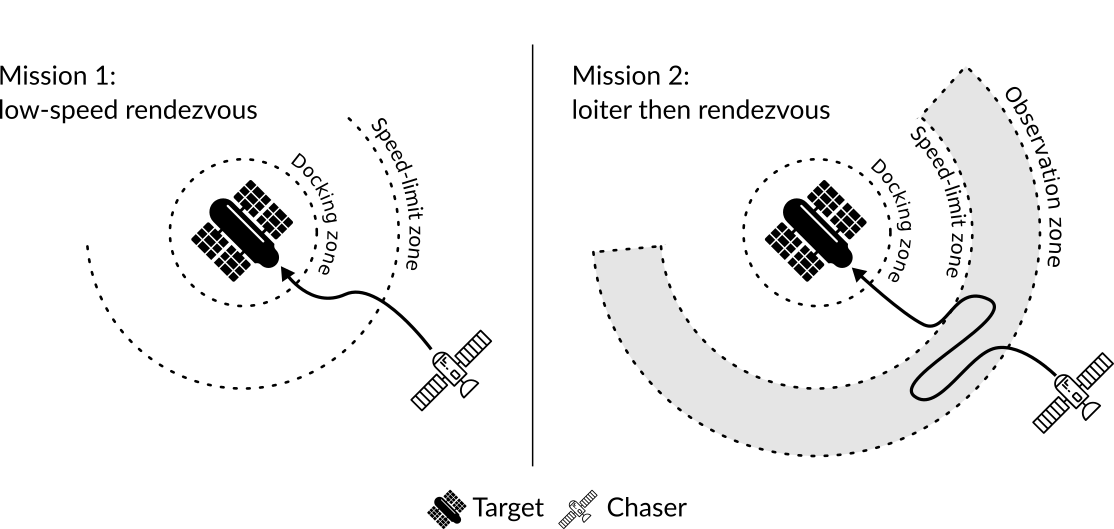
\includegraphics[width=\linewidth]{images/iros/satellite_missions.png}
	\caption{Two satellite rendezvous missions used in our experiments. In the first mission, the chaser satellite must eventually reach the target while respecting a maximum speed constraint in the region immediately around the target. In the second mission, the chaser must still reach the target and obey the speed limit, but it must also loiter in an observation region for some minimum time before approaching. The first mission requires an STL formula with three predicates and three temporal operators, while the second mission requires five predicates and five temporal operators. Figure \textcopyright{} IEEE 2022; used with permission.}
	\label{ch:iros:fig:mission_specs}
\end{figure}

For each mission, the design parameters $\theta$ define the planned trajectory for the chaser (represented as state and input waypoints) as well as the feedback control gains used to track that trajectory, while the exogenous parameters $\phi$ represent bounded uncertainty in the initial state of the chaser ($p_x(0), p_y(0) \in [10, 13]$, $p_z(0) \in [-3, 3]$, $v_x(0), v_y(0), v_z(0) \in [-1, 1]$). We simulate both missions for \SI{200}{s} with a \SI{2}{s} timestep. For each mission, we include a penalty on the total impulse $I$ (in Newton-seconds) required for the maneuver, with $J_\psi = \rho(\psi, S(\theta, \phi), 0) + \lambda I$ and $\lambda = 5\times10^{-5}$.

\subsection{Baselines}

We compare our approach against two baselines: an MIP planner based on that in~\cite{raman15} and~\cite{sadraddiniRobustTemporalLogic2016} and the nonlinear optimization approach from~\cite{pantSmoothOperatorControl2017,pantazidesSatelliteMissionPlanning2022}.

The MIP approach uses a model-predictive control formulation, and~\cite{raman15} proposes to add counterexamples after solving each instance of the problem. Due to the large size of the resulting MIPs (2800-4500 integer variables for these case studies), we could not find an optimal solution for either satellite problem within 1 hour. Because we were not able to solve even a single instance of the MIP planning problem, we were not able to solve it multiple times to generate any MIP-generated counterexamples. For the comparisons below, we take the best feasible solution found after \SI{500}{s} for the first mission and \SI{1000}{s} for the second mission.

We also compare with extensions of the nonlinear optimization method from~\cite{pantSmoothOperatorControl2017,pantazidesSatelliteMissionPlanning2022} that include domain randomization with either 32 or 64 samples of $\phi$. These methods are similar to those proposed in~\cite{leungBackPropagationSignalTemporal2021}, but we re-implement the method to ensure a fair comparison (our implementation uses just-in-time compilation to speed up gradient computation, resulting in a speed increase over the original implementation). We use the same cost function as in our method, with the same penalty on total impulse.

In the following, we denote our method as CG (counterexample-guided), the nonlinear optimization methods as NLopt (with additional notation for the number of domain randomization examples), and the mixed integer programming method as MIP.

\subsection{Results}

Figs.~\ref{ch:iros:fig:mission_1_comparison} and~\ref{ch:iros:fig:mission_2_comparison} show the results of solving the first and second missions, respectively, with each method. In all cases, we compare the results starting the optimization process from 50 random seeds, reporting the time required and the robustness of the optimized plan under an adversarial disturbance computed via local gradient ascent against the optimal solution. Experiments are run on a laptop computer with \SI{8}{GB} of RAM and a \SI{1.8}{GHz} 8-core CPU.

\begin{figure}[tbh]
	\centering
	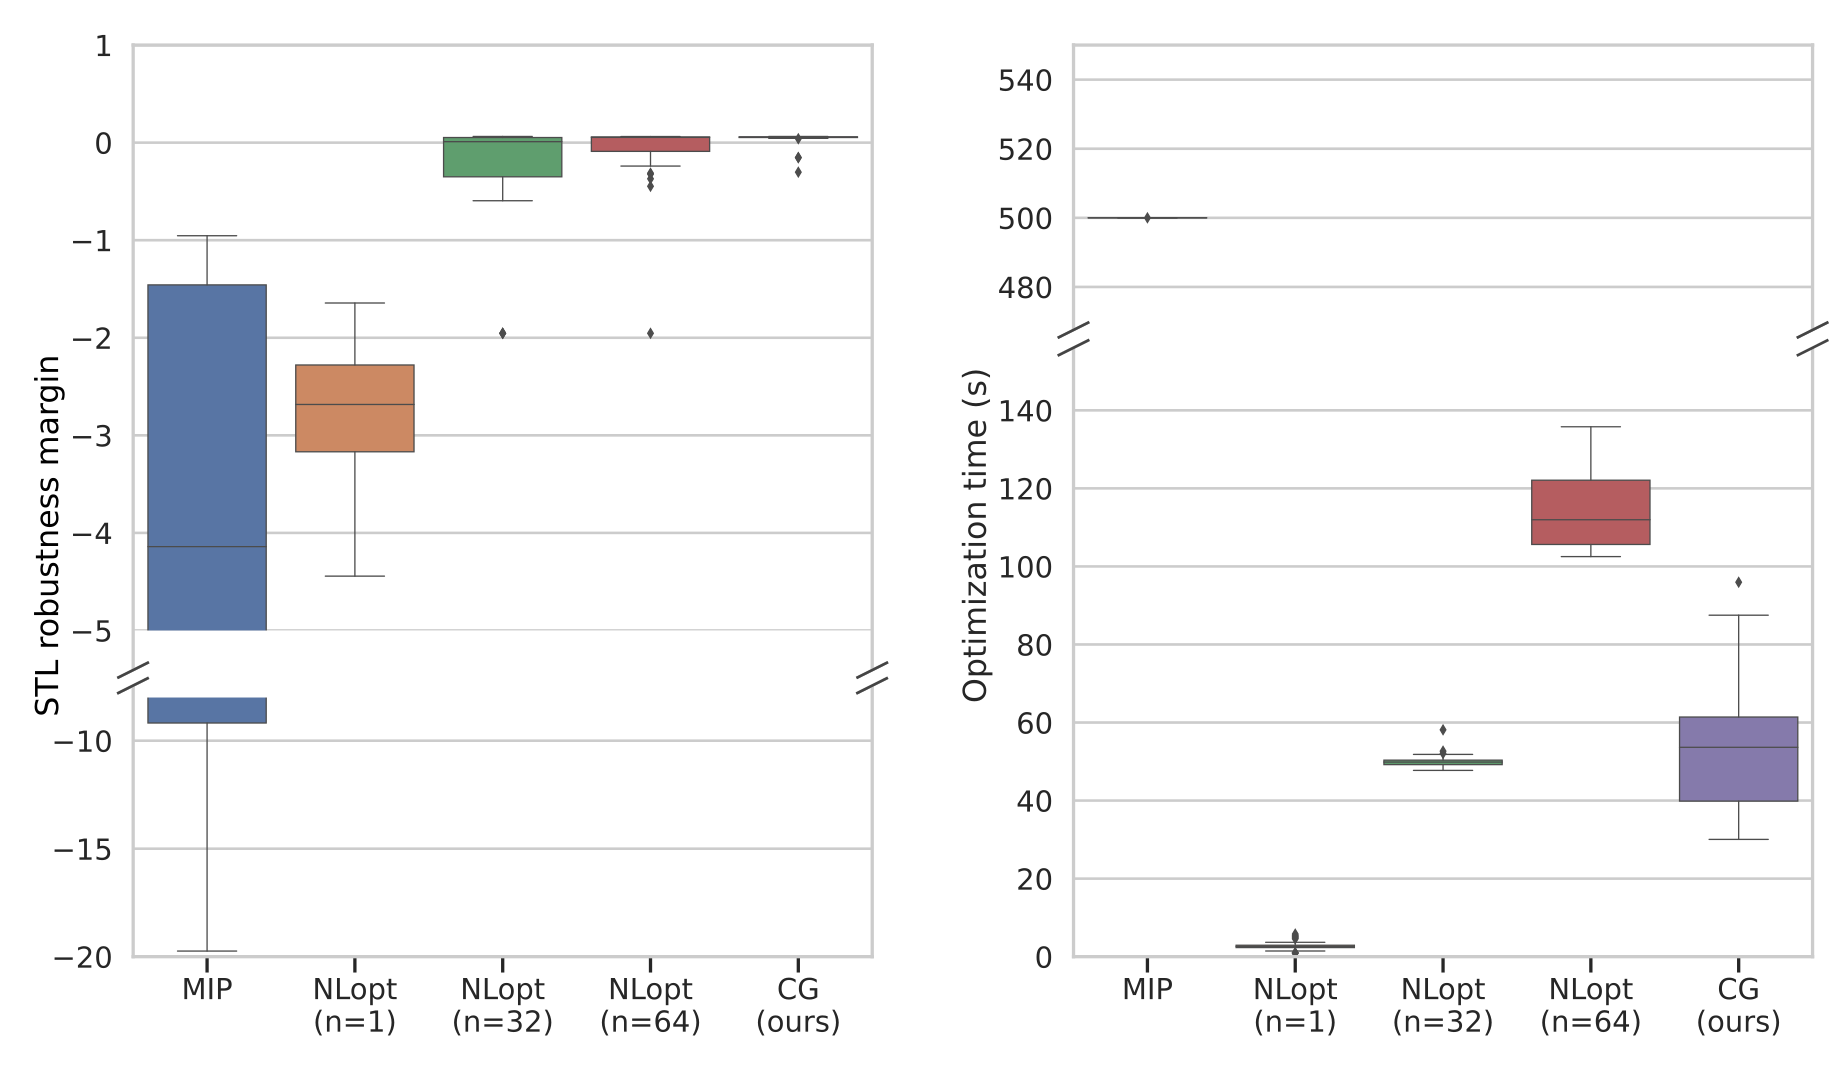
\includegraphics[width=\linewidth]{iros/mission_1_comparison.png}
	\caption{Comparison of different STL planning methods on the first example mission, averaged over 50 random seeds. Left: the robustness margin $\rho(\psi_1)$ computed for the optimized design parameters and worst-case exogenous parameters. Right: the planning time required by each method. Our method (CG) achieves much higher robustness than all other methods (satisfying the STL specification despite adversarial perturbations in all but 3 instances) and runs twice as fast as the next-most-robust method. Figure \textcopyright{} IEEE 2022; used with permission.}
	\label{ch:iros:fig:mission_1_comparison}
\end{figure}

\begin{figure}[tbh]
	\centering
	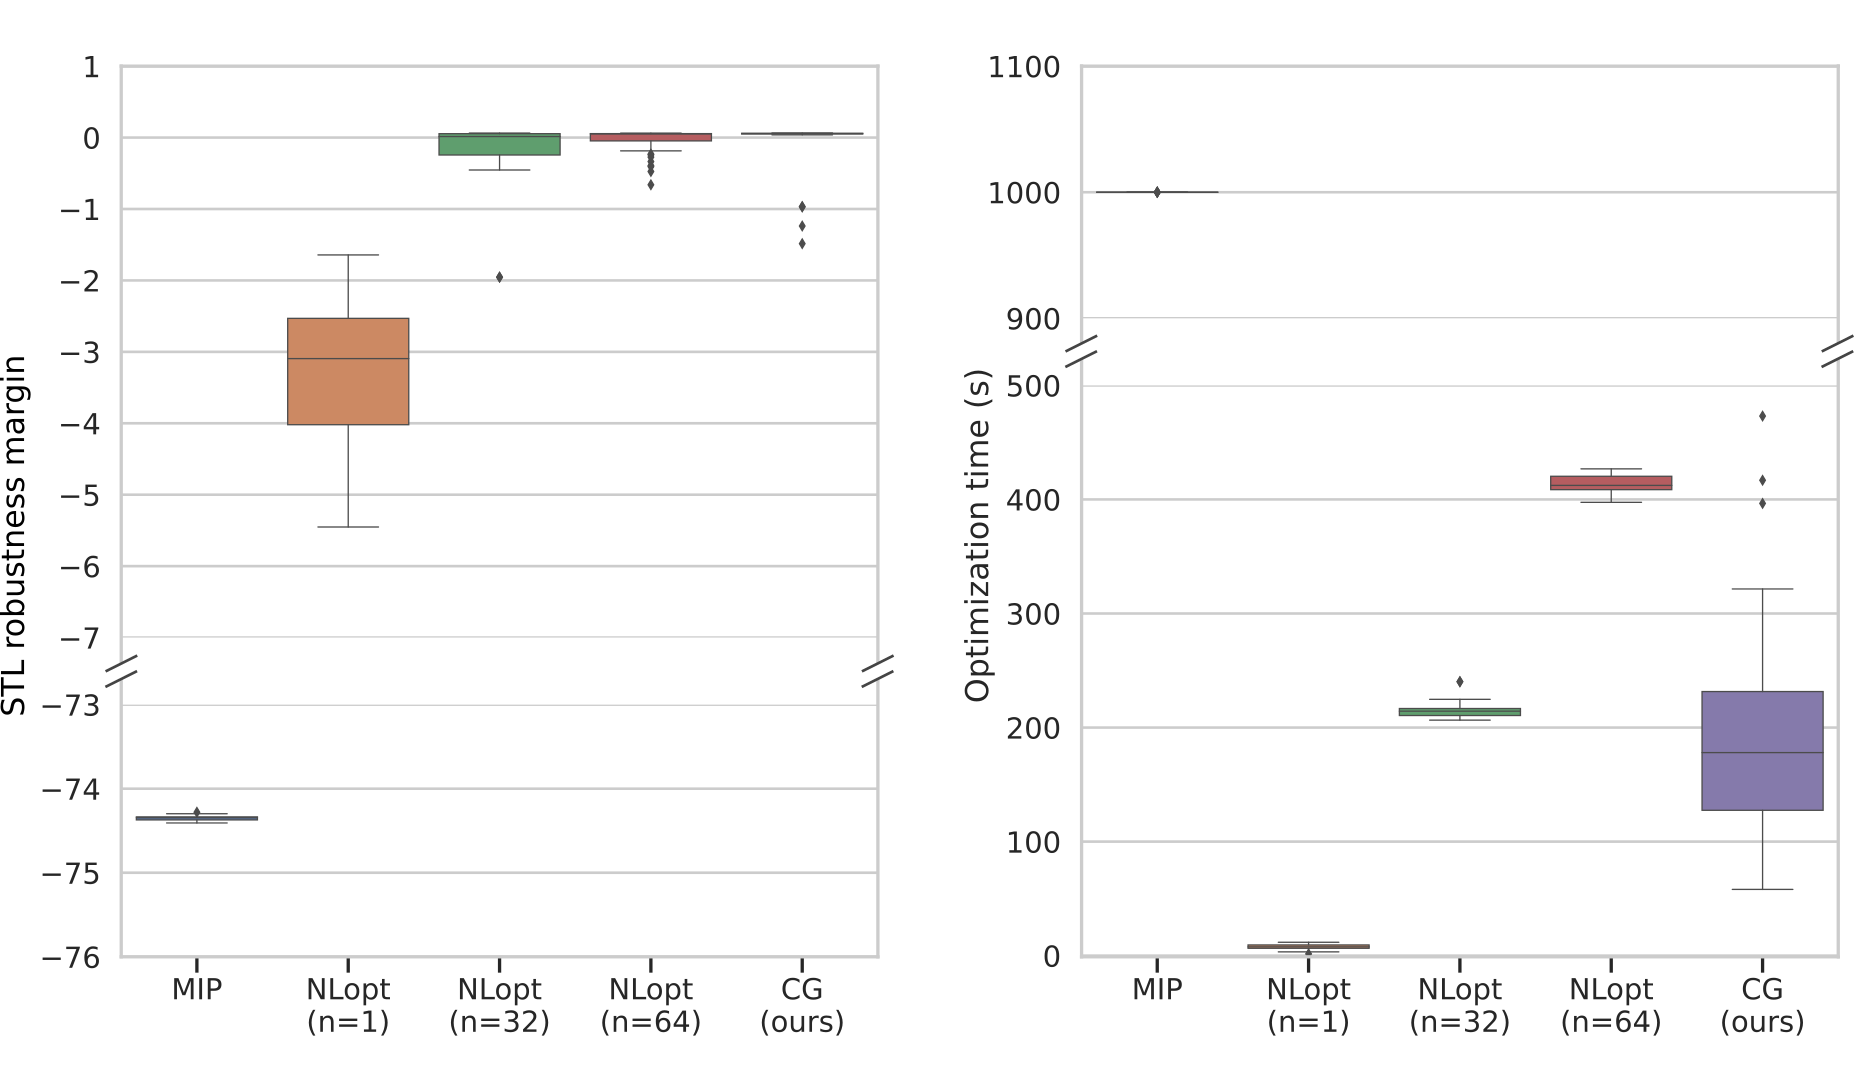
\includegraphics[width=\linewidth]{iros/mission_2_comparison.png}
	\caption{Comparison of different STL planning methods on the second example mission, averaged over 50 random seeds. Left: the robustness margin $\rho(\psi_2)$ computed for the optimized design parameters and worst-case exogenous parameters. Right: time required by each method to find a plan. Our method (CG) finds much more robust plans, satisfying the specification in all but 4 instances compared to 17 failures for the next-best method (NLopt with 64 examples). Our method also runs more than twice as fast as the next-most-robust method. Figure \textcopyright{} IEEE 2022; used with permission.}
	\label{ch:iros:fig:mission_2_comparison}
\end{figure}

Across both missions, we find that our method consistently yields more robust plans than prior methods. In the first mission, our method finds designs that satisfy the STL specifications in all but 3 trials despite the worst-case adversarial disturbance (an example trajectory is shown in Fig.~\ref{ch:iros:fig:mission_1_traj}), while the next-best method (NLopt with 64 domain randomization samples) fails on 14 out of 50 trials and takes more than twice as long to run (\SI{114.3}{s} vs. \SI{53.7}{s} for our method). These results demonstrate the importance of using high-quality counterexamples during optimization: instead of 64 random samples, our method uses 8 initial random samples and 1--4 (median 2) additional counterexamples found using Algorithm~\ref{ch:iros:alg:cg_gs}. Because the MIP cannot practically be solved multiple times to consider variation in $\phi$, the solutions found using the MIP method tend to be less robust; moreover, MIP failed to find a feasible solution for the first mission within \SI{500}{s} in 16 out of 50 trials.

Our method also performs well on the second mission, satisfying the STL requirement on 46 out of 50 random trials; a representative trajectory is shown in Fig.~\ref{ch:iros:fig:mission_2_traj}. Despite an additional \SI{500}{s} of solving time, the MIP method fails to find a feasible solution in $16$ out of 50 trials (the MIP encoding requires 2806 binary variables). The second-most-robust method, after ours, is NLOpt with 64 random examples; this method fails to find a design that satisfies the STL requirement on 17 out of 50 trials despite taking twice as long to run as our method (which required a median of 2 iterations of Algorithm~\ref{ch:iros:alg:cg_gs}).

\begin{figure}[tbh]
	\centering
	\begin{subfigure}[b]{0.45\linewidth}
		\centering
		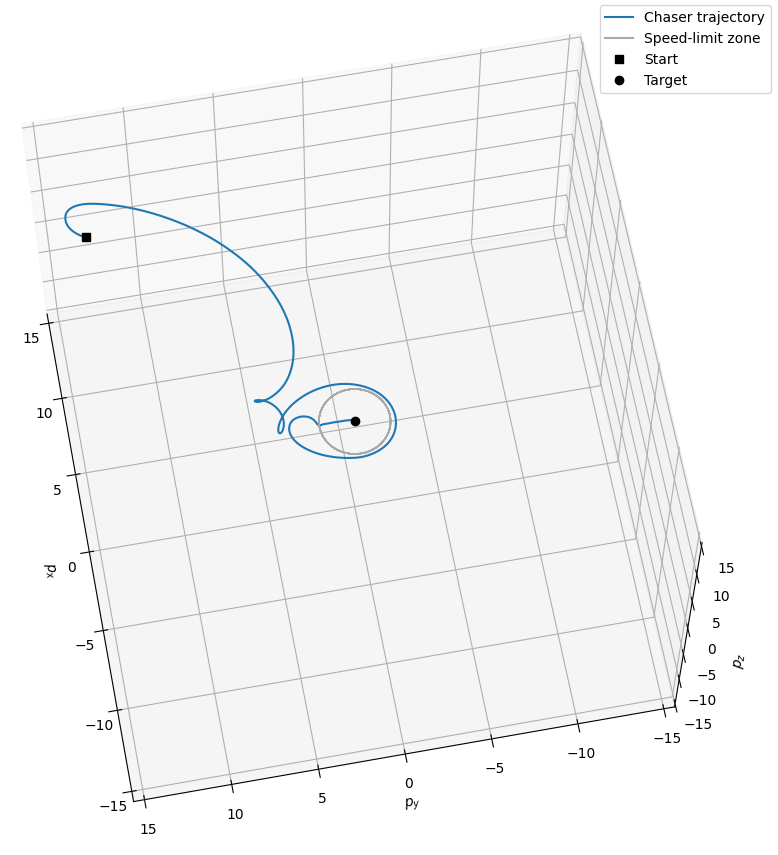
\includegraphics[width=0.9\linewidth]{iros/satellite_mission1_traj.png}
		\caption{Mission 1.}
		\label{ch:iros:fig:mission_1_traj}
	\end{subfigure}
	\quad
	\begin{subfigure}[b]{0.45\linewidth}
		\centering
		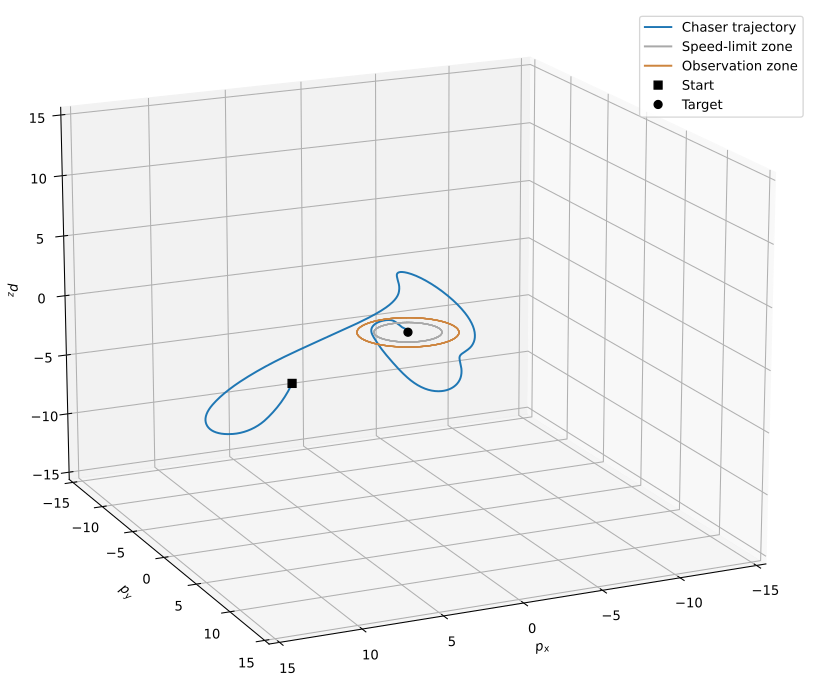
\includegraphics[width=\linewidth]{iros/satellite_mission2_traj.png}
		\caption{Mission 2.}
		\label{ch:iros:fig:mission_2_traj}
	\end{subfigure}
	\caption{Optimized trajectories found using our method for the two satellite rendezvous missions. Figures \textcopyright{} IEEE 2022; used with permission.}
\end{figure}

\section{Summary}

In this chapter, we describe a counterexample-guided approach to end-to-end robot design optimization with formal behavior specifications. This chapter closes two gaps that were left open in Chapter~\ref{ch:rss}. First, by using STL to directly specify the desired behavior, we avoid the need for manual reward design. Second, we consider robustness to worst-case disturbances at design time using counterexample-guided adversarial optimization (rather than the post-hoc statistical method from Chapter~\ref{ch:rss}).

Our empirical results show that our adversarial optimization method yields optimized designs that are more robust than those found by competing methods, despite requiring substantially less computational effort than the next-best method. That said, all methods described in this chapter (aside from intractable MIP-based methods) are inherently local; they rely on local optimization to find both promising designs and adversarial counterexamples. As a result, there is a risk that our method, and any other method that relies on local gradient-based optimization, will get stuck in a local optimum. At first glance, this sub-optimality might not seem like a large issue, since local optimization methods have been successful in many robotics and learning applications~\cite{dawsonCertifiableRobotDesign2022}. Unfortunately, for safety-critical applications, a sub-optimal counterexample is potentially worse than no counterexample at all. This is because a sub-optimal counterexample --- i.e. an artificially easy test case --- can lead to false negatives where we erroneously believe that we have mitigated the worst-case disturbance. We can see this issue manifest in Figs.~\ref{ch:iros:fig:mission_1_comparison} and~\ref{ch:iros:fig:mission_2_comparison} in the few failures that remain even after Algorithm~\ref{ch:iros:alg:cg_gs} converges. In these cases, Algorithm~\ref{ch:iros:alg:cg_gs} has converged to a local Nash equilibrium and has not correctly identified the true worst-case disturbance.

In the next chapter, we will introduce a novel reformulation of the counterexample-guided optimization problem that addresses this issue. By combining (approximately) global probabilistic inference methods with gradients from differentiable simulation, we can find more challenging counterexamples that will lead to correspondingly more robust designs.
\chapter{Gradient-accelerated Inference for Diverse Counterexamples}\label{ch:corl}

In Chapters~\ref{ch:rss} and~\ref{ch:iros}, we introduce local gradient-based optimization methods for design, using standard optimization and adversarial verification-guided optimization. As discussed at the end of Chapter~\ref{ch:iros}, there are a few drawbacks inherent to local methods.

\begin{enumerate}
    \item \textbf{Risk of local minima: } Local gradient-based optimizers are greedy and prone to getting stuck in local minima. This risk is particularly important in safety-critical use cases, since converging to a counterexample that is far from the true worst-case might lead us to falsely believe that a design is safe.
    \item \textbf{Lack of diversity in adversarial examples: } When verifying a system, it is important to consider a diverse set of failure modes. However, optimization-based approaches have difficulty balancing exploration with exploitation; nearby solutions will typically converge to the nearest local optimum.
    \item \textbf{Sensitivity to gradient quality: } Many robotic systems, particularly those involving contact or vision, have dynamics that are not differentiable everywhere, as we assumed in previous chapters. Even when these dynamics are smoothed, there are still regions where the gradients can be poorly conditioned (i.e. arbitrarily large) or flat, which will cause a gradient-based optimizer to diverge or get stuck.
\end{enumerate}

These drawbacks have prompted much discussion in the literature on the limitations of differentiable simulation as a design tool, particularly since certain robotics applications with contact-rich dynamics~\cite{suhDifferentiableSimulatorsGive2022,metzGradientsAreNot2022} or vision in the loop~\cite{zhaoPhysicsbasedDifferentiableRendering2020} can yield poorly conditioned gradients. This has lead to prior work on safety verification for systems with vision in the loop to learn an approximate proxy model for the vision component~\cite{sinhaNeuralBridgeSampling2020} (where it can be difficult to gather enough training data for rare failure events) or skip the rendering step entirely during backpropagation~\cite{hanselmannKINGGeneratingSafetyCritical2022a} (which makes it difficult to repair visual-feedback policies).

In this chapter, we address these drawbacks by re-framing the counterexample-guided optimization problem from Chapter~\ref{ch:iros} as a Bayesian inference problems, which we then solve using gradient-accelerated Markov Chain Monte Carlo (MCMC) methods. We demonstrate empirically how this Bayesian inference framework provides improved performance (in both convergence speed and solution quality) over both gradient-based and gradient-free optimization methods, and we provide a theoretical analysis to support these empirical observations. We also provide a gradient-free variant of our method for use in cases when a differentiable simulator is not available. This chapter is based in part on the author's published work in~\cite{dawsonBayesianApproachBreaking2023}.

The probabilistic approach presented in this chapter builds off of prior work on inference as a verification tool. \cite{okellyScalableEndtoEndAutonomous2018} propose an end-to-end verification tool for autonomous vehicles based on gradient-free adaptive importance sampling. \cite{zhouRoCUSRobotController2021} use gradient-free Markov Chain Monte Carlo (MCMC) to find counterexamples. \cite{sinhaNeuralBridgeSampling2020} and \cite{deleckiModelbasedValidationProbabilistic2023a} use gradient-based MCMC to estimate the risk of failure and find counterexamples, respectively.
%
These prior works are focused only on predicting failure modes; they are not able to improve the system (e.g. by re-optimizing the controller) to fix these failures once they have been discovered. Our method aims to fill this gap by combining failure mode prediction and repair, exploiting the duality between these problems to efficiently search for both a diverse set of counterexamples and updates to the system's policy or design that reduces the severity of those failures.

\section{From optimization to inference}

To motivate the switch from optimization to inference, consider the toy example of optimizing the cost landscape shown on the left in Fig.~\ref{ch:corl:fig:toy_example}. This cost function has local minima at $x = -0.544$ (marked with a square) and $x = 0.919$ (the true global optimum, marked with a circle). If initialized with $x < 0$, a local gradient-based optimizer will naturally converge to the sub-optimal local minimum at $x = -0.544$, missing the global minimum. We can see this behavior in Fig.~\ref{ch:corl:fig:toy_example_convergence}, which plots the convergence of gradient-based optimization with 5 different random starting positions $x\sim\cN(-1.5, 0.1)$. All 5 runs converge to the suboptimal local minimum at $x = -0.544$.

To avoid getting stuck in this local minimum, we can convert this optimization problem into an inference problem; i.e. sampling from the unnormalized probability density:
\begin{align*}
    \argmin_x U(x) \quad \implies \quad x \sim p(x) \propto e^{-U(x)}
\end{align*}
%
This unnormalized distribution is shown on the right in Fig.~\ref{ch:corl:fig:toy_example}. We can see that the distribution is bimodal, with a peak at the suboptimal local minimum and a larger peak at the global minimum. By sampling from this distribution, we can find the global minimum with high probability (this is the so-called \textit{Optimization as Inference} perspective~\cite{maSamplingCanBe2019,levineReinforcementLearningControl2018a}). In practice, we can approximately sample from this distribution using Markov Chain Monte Carlo (MCMC) methods, which we will discuss in more detail shortly. The benefit of these methods is that they balance exploring different regions of the distribution with exploiting high-likelihood areas. We can see this behavior in Fig.~\ref{ch:corl:fig:toy_example_convergence}, which shows the convergence of Metropolis-adjusted Langevin (MALA) MCMC, a gradient-based inference method, on the same cost landscape over 5 different random seeds. MALA is able to find the global minimum with high probability, while gradient-based optimization gets stuck in the local minimum.

\begin{figure}[tb]
    \centering
    \begin{subfigure}[b]{\linewidth}
        \centering
        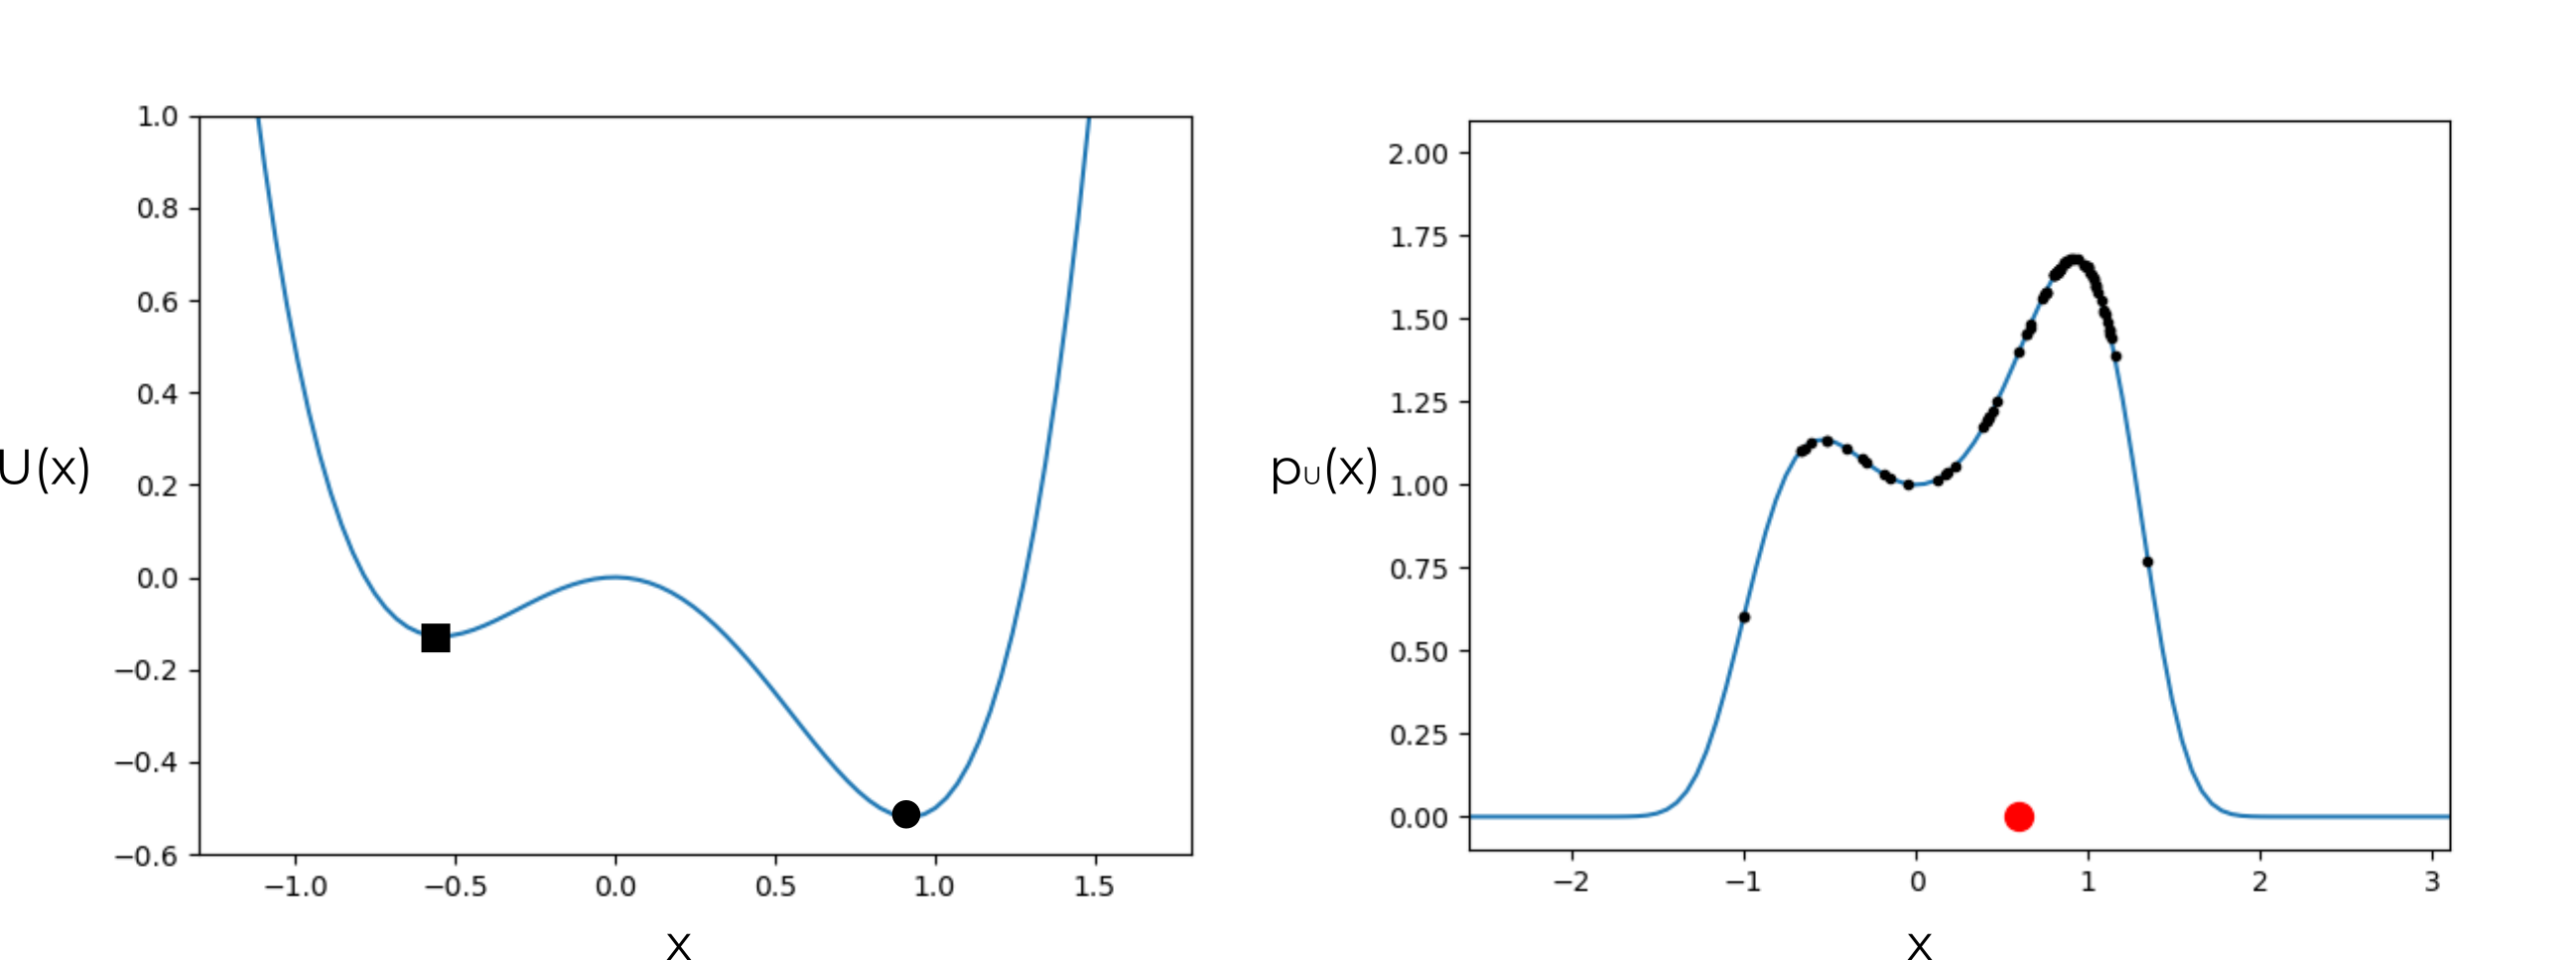
\includegraphics[width=0.7\linewidth]{images/global_methods/sampling_as_optimization.png}
        \caption{Left: a bimodal cost landscape $U(x) = x^4 - 0.5 x^3 - x^2$ with a local optimum at $x\approx -0.544$ and a global optimum at $x\approx 0.919$. Right: the corresponding unnormalized likelihood $p(x) \propto e^{-U(x)}$, samples drawn from this distribution (black dots), and the average of 100 samples (red dot).}
        \label{ch:corl:fig:toy_example}
    \end{subfigure}
    \begin{subfigure}[b]{\linewidth}
        \centering
        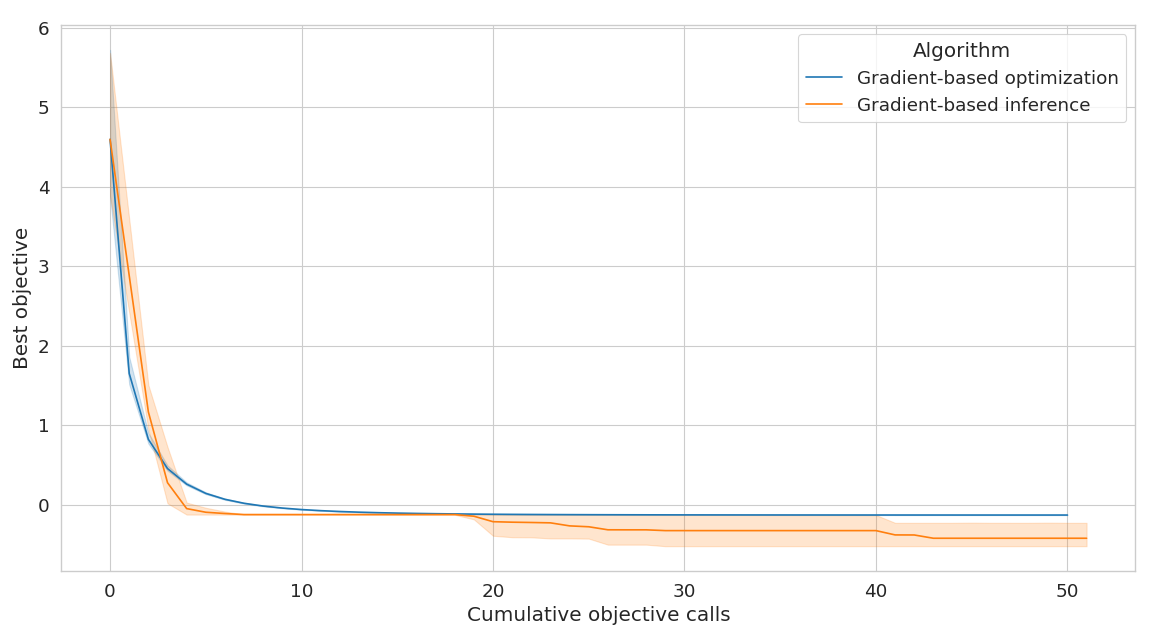
\includegraphics[width=0.7\linewidth]{images/global_methods/double_well_gd_mala.png}
        \caption{Convergence of gradient-based optimization and inference (Metropolis-adjusted Langevin) on the double-well cost landscape from Fig.~\ref{ch:corl:fig:toy_example}, showing how the optimization method gets stuck in a local minimum while the inference method is able to escape and find the global minimum.}
        \label{ch:corl:fig:toy_example_convergence}
    \end{subfigure}
    \caption{A simple example demonstrating the use of MCMC on multimodal optimization problems.}
\end{figure}

A wide variety of MCMC algorithms exist to sample from arbitrary non-normalized probability distributions~\cite{geyerIntroductionMarkovChain2011}; common variants include Random-walk Metropolis-Hastings (RMH), Hamiltonian Monte Carlo (HMC), unadjusted Langevin (ULA), and MALA. RMH is gradient-free, while HMC, ULA, and MALA are gradient-based. MALA, which can be seen as a single-step version of HMC, is outlined in Algorithm~\ref{ch:corl:alg:mala}. Like all MCMC algorithms, it defines a Markov chain with a transition rule designed to preserve the so-called detailed balance condition, which ensures that the stationary distribution of the Markov chain is the same as the target density (see~\cite{geyerIntroductionMarkovChain2011,aiama} for a more complete introduction). MALA defines a transition rule that begins by proposing a candidate state in line~\ref{ch:corl:alg:mala:step} using a gradient-driven drift term and a Gaussian diffusion term. The candidate state is accepted with probability $P_{accept}$ in line~\ref{ch:corl:alg:mala:mh}, which is proportional to the ratio of the target density at the candidate and current states. If the candidate state is accepted, it becomes the new current state; otherwise, the current state is repeated. The algorithm is run for $K$ steps, and the final state is returned as the sample from the target density.

\begin{algorithm}
    \caption{Metropolis-adjusted Langevin algorithm (MALA,~\cite{maSamplingCanBe2019,robertsLangevinDiffusionsMetropolisHastings2002})\label{ch:corl:alg:mala}}
    \DontPrintSemicolon
    \KwInput{Initial $x_0$, steps $K$, stepsize $\epsilon$, density $p(x)$.}
    \KwOutput{A sample drawn from $p(x)$.}
    \For{$i = 1, \ldots, K$}
    {
    Sample $\eta \sim \cN(0, 2\epsilon I)$ \Comment{Gaussian noise}\;
    $x_{i+1} \gets x_i + \epsilon \nabla \log p(x_i) + \eta$ \Comment{Propose next state}\;\label{ch:corl:alg:mala:step}
    $P_{accept} \gets \frac{p(x_{i+1}) e^{-||x_i - x_{i+1} - \epsilon \nabla \log p(x_{i+1})||^2 / (4\epsilon)}}{p(x_{i}) e^{-||x_{i+1} - x_{i} - \epsilon \nabla \log p(x_{i})||^2 / (4\tau)}}$ \;
    With probability $1 - \min(1, P_{accept})$:
    \hspace{2em}$x_{i+1} \gets x_{i}$ \Comment{Accept/reject proposal}\;\label{ch:corl:alg:mala:mh}
    }
    \KwRet{$x_K$}
\end{algorithm}

We have shown how transitioning from gradient-based optimization to inference (in particular, gradient-based inference using MALA) addresses the first drawback identified at the start of this chapter (the risk of getting stuck in local minima). Next, we will discuss how gradient-based inference also addresses the other two drawbacks (the difficulty of sampling diverse failure modes and sensitivity to gradient quality).

\subsection{Sampling diverse solutions}

MCMC sampling methods provide a principled means for balancing exploration and exploitation, and so they are well-suited to problems with multiple modes (particularly when the modes are close together in the search space). However, although MCMC methods enjoy good asymptotic guarantees, including ergodicity and convergence to the target distribution in the infinite-sample limit, any finite-sample implementation will struggle to explore a highly multi-modal target distribution if the modes are well separated (any finite MCMC run will be biased towards the modes near its starting point). A family of algorithms known as sequential Monte Carlo (SMC) algorithms exist to solve this problem by smoothly interpolating between a sequence of distributions, starting from a simple distribution (e.g., a Gaussian) and ending at the target distribution~\cite{chopinIntroductionSequentialMonte2020}. SMC algorithms are particularly useful for inference problems with multiple modes, since they can be used to sample from the target distribution in a way that is less biased by the initialization. In the following section, we will discuss how SMC can be applied to sample diverse solutions (both failure modes and designs) for practical autonomous system design and verification problems.

\subsection{Sensitivity to gradient quality}

As discussed at the start of this chapter and in prior work~\cite{suhDifferentiableSimulatorsGive2022,suh2021_bundled_gradients}, many practical robotics problems involve non-smooth dynamics that may not be differentiable, or even continuous, at all points. For example, dynamics involving rigid body contact are discontinuous at the point when contact is made or broken~\cite{suhDifferentiableSimulatorsGive2022}, and many image rendering algorithms are not directly differentiable~\cite{zhaoPhysicsbasedDifferentiableRendering2020}. Even when these functions can be smoothed, they may still have poorly behaved gradients (e.g. gradients that are either flat or very large). Prior work~\cite{suhDifferentiableSimulatorsGive2022} identifies the ballistic optimization problem shown in Fig.~\ref{ch:corl:fig:ballistic} as a simple problem that illustrates the effect of both flat gradients and discontinuities.

Fig.~\ref{ch:corl:fig:ballistic_convergence} shows the cost of the best solution found by local optimization using gradient descent, inference using MALA (a gradient-based method), and inference using RMH (a gradient-free method), all starting from a point left of the flat region. As expected, we see that gradient descent gets stuck in the flat region, but both inference methods are able to explore the flat region and eventually discover the global optimum. A natural next question is whether and to what extent gradients help the inference methods explore this distribution; to answer this question, we define a high-dimensional version of the ballistic problem that simply runs $N$ instances in parallel (using an $N$-dimensional decision vector with one element for each instance) and returns the total cost across all problems. In low dimensions, there is no discernible difference between the gradient-free and gradient-based inference methods. In higher dimensions $N > 10$, gradient-free RMH does not even reach the flat region where gradient descent gets stuck, while gradient-based MALA converges even in $N=1000$ dimensions.

We attribute this improved performance to three factors. First, the Gaussian diffusion term in the MALA proposal allows it to explore the flat region of the cost landscape and eventually find the optimal solution. Second, the accept/reject step provides some robustness to stiff or inaccurate gradients; if a bad gradient causes MALA to propose a state with much higher cost (lower likelihood), then it will likely reject that proposal and try again. Third, the gradient-based drift term in the proposal provides a valuable heuristic for exploring high-dimensional space, where the exponentially decreased volume of the region around the optimal solution makes it difficult to explore using gradient-free methods.

\begin{figure}[t]
    \centering
    \begin{subfigure}[t]{0.6\linewidth}
        \centering
        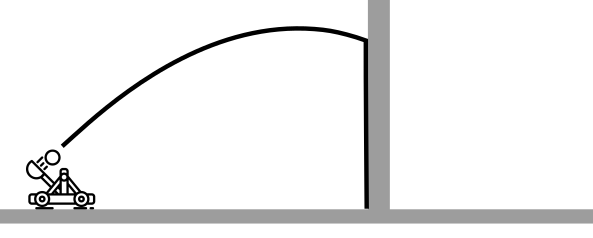
\includegraphics[width=\linewidth]{images/global_methods/ballistic.png}
    \end{subfigure}
    \begin{subfigure}[t]{0.3\linewidth}
        \centering
        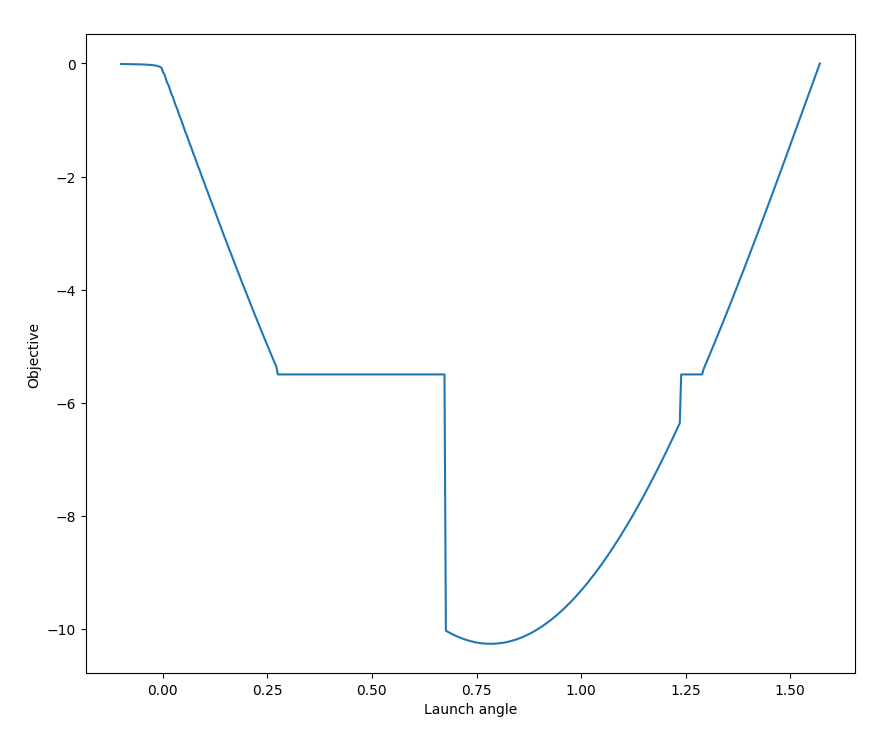
\includegraphics[width=\linewidth]{images/global_methods/ballistic_cost.png}
    \end{subfigure}%
    \caption{Left: the ballistic optimization problem from~\cite{suhDifferentiableSimulatorsGive2022}. Right: the corresponding cost landscape.}
    \label{ch:corl:fig:ballistic}
\end{figure}

\begin{figure}[tb]
    \centering
    \begin{subfigure}[t]{0.24\linewidth}
        \centering
        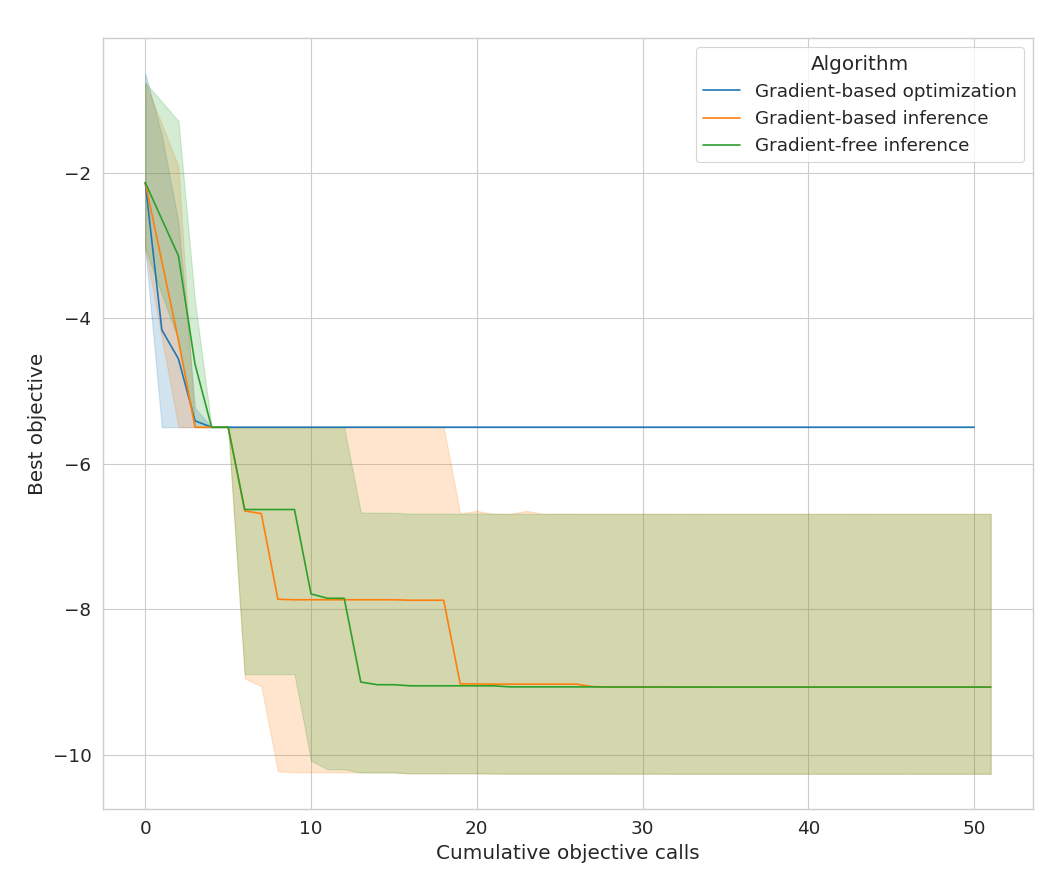
\includegraphics[width=\linewidth]{images/global_methods/ballistic_1.png}
        \caption{$N=1$}
    \end{subfigure}
    \begin{subfigure}[t]{0.24\linewidth}
        \centering
        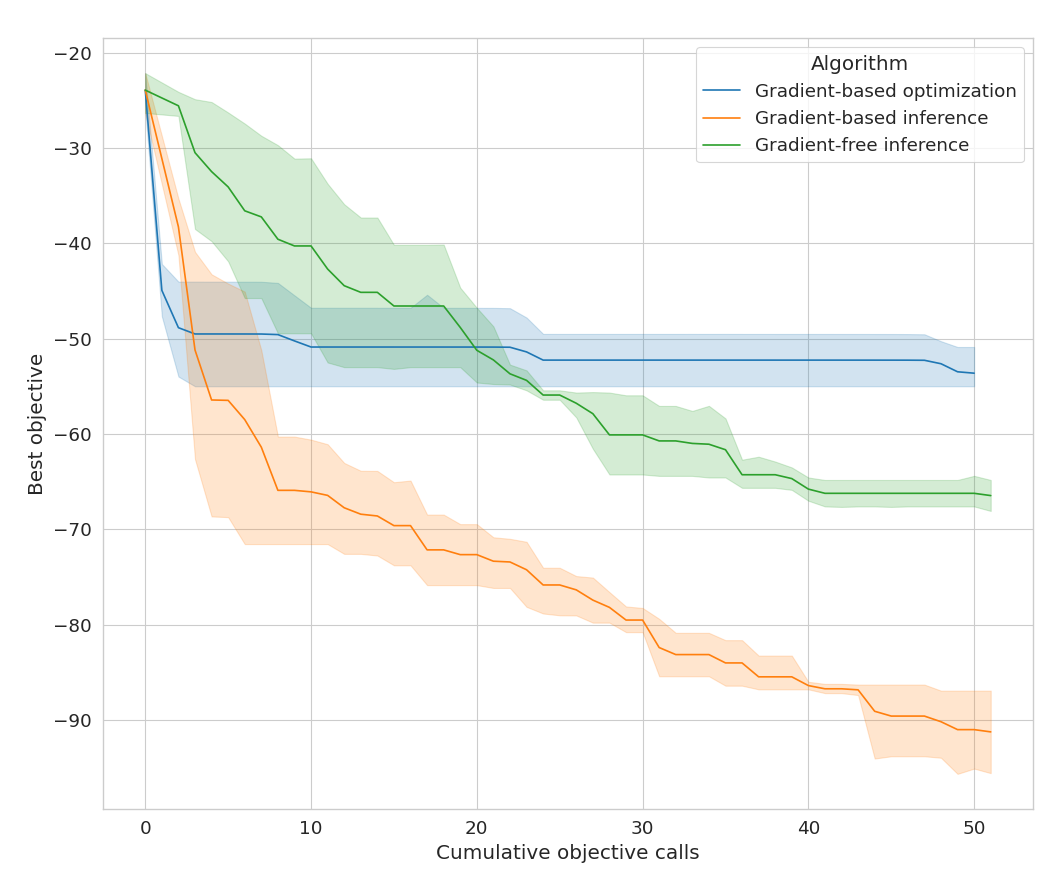
\includegraphics[width=\linewidth]{images/global_methods/ballistic_10.png}
        \caption{$N=10$}
    \end{subfigure}
    \begin{subfigure}[t]{0.24\linewidth}
        \centering
        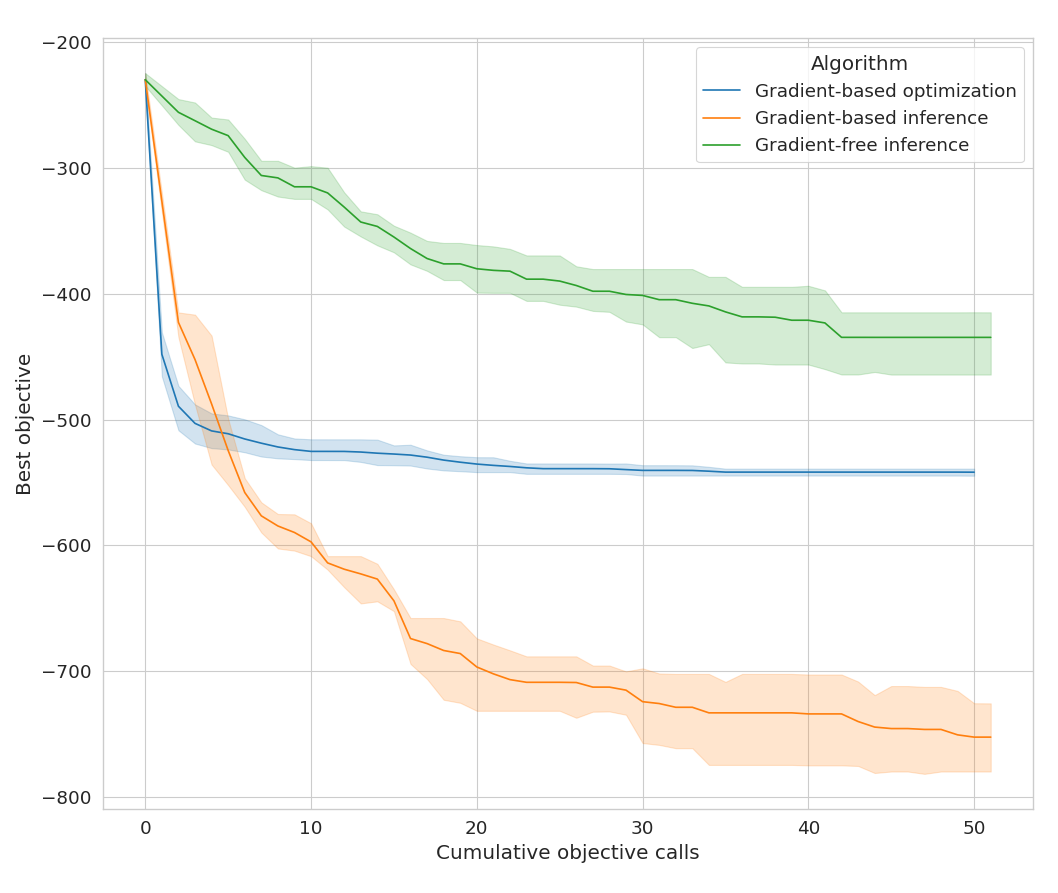
\includegraphics[width=\linewidth]{images/global_methods/ballistic_100.png}
        \caption{$N=100$}
    \end{subfigure}
    \begin{subfigure}[t]{0.24\linewidth}
        \centering
        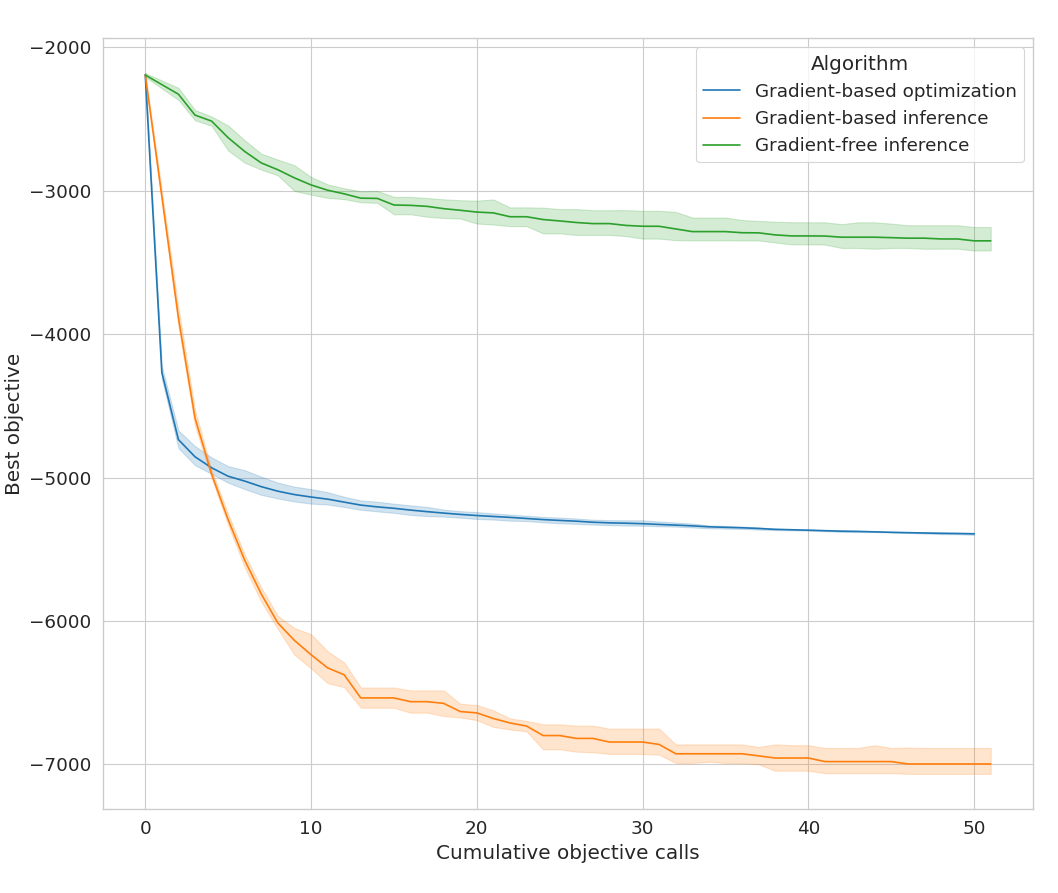
\includegraphics[width=\linewidth]{images/global_methods/ballistic_1000.png}
        \caption{$N=1000$}
    \end{subfigure}
    \caption{Convergence of gradient-based optimization (gradient descent), gradient-based inference (MALA), and gradient-free inference (RMH) on the ballistic cost landscape from Fig.~\ref{ch:corl:fig:toy_example}.}
    \label{ch:corl:fig:ballistic_convergence}
\end{figure}

\section{Sampling and repairing diverse failure modes}

Now that we have motivated the switch from optimization to inference, we will reframe the adversarial optimization from Chapter~\ref{ch:iros} as a sequential inference problem, then demonstrate how we can used gradient-accelerated MCMC sampling (i.e. MALA) to efficiently sample diverse failure modes and find more robust optimized designs.

\subsection{Preliminaries}

Let us define a ``failure mode'' as a set of environmental parameters $\phi$ that induce high cost for given policy parameters $\theta$, i.e. finding multiple solutions $\phi^*(\theta) = \text{find}_\phi J(\theta, \phi) \geq J^*$ for failure threshold $J^*$. In this context, \textit{failure prediction} is the search for such $\phi^*$ given a design $\theta$, while \textit{failure repair} is the search for updated design parameters $\theta^*$ that achieve low costs despite possible variation in $\phi$. Note that this is a slightly different framing than used in the adversarial setting in Chapter~\ref{ch:iros} due to the use of a cost threshold, which is intended to encourage diversity in the predicted failure modes and makes our theoretical analysis later in this chapter more straightforward.

In the following, we will frame the failure prediction and repair in the language of Bayesian inference. We assume that $\phi$ are distributed according to some prior distribution $p_{\phi, 0}$; unlike in Chapter~\ref{ch:rss}, we assume the ability to evaluate and automatically differentiate $\log p_{\phi, 0}$. Similarly, we assume knowledge of a prior over design parameters $p_{\theta, 0}$, which is used to regularize the design parameters during the repair process.

Given this context, \textit{failure prediction} entails sampling from a pseudo-posterior distribution that balances the prior likelihood of a disturbance with the severity of the induced failure:
%
\begin{equation}
    p_{\rm{failure}}(\phi; \theta) \propto p_{\phi, 0}(\phi)e^{-[J^* - J(\theta, \phi)]_+} \label{ch:corl:eq:failure_logprob_basic}
\end{equation}
%
where $J^*$ is the cost threshold for a failure event and $[\cdot]_+$ is the exponential linear unit. Intuitively, we can interpret this likelihood as a posterior over environmental parameters $\phi$ conditioned on a failure occurring \cite{sinhaNeuralBridgeSampling2020,zhouRoCUSRobotController2021,maSamplingCanBe2019,dawsonBayesianApproachBreaking2023}. By framing the search for failures prediction as a sampling problem, rather than the traditional adversarial optimization, we gain advantages discussed in the previous section, including the ability to sample diverse failure modes and robustness to poorly conditioned gradients.

This is not the first paper to take a sampling-based approach to failure prediction; for example, \cite{okellyScalableEndtoEndAutonomous2018}, \cite{sinhaNeuralBridgeSampling2020}, and \cite{zhouRoCUSRobotController2021} also approach failure prediction using this lens. One of our key insights is that this sampling framework can be extended to not only predict failures but also repair the underlying policy, thus mitigating the impact of the failure.
%
Given initial design parameters $\theta_0$ and a population of anticipated failure modes $\phi_1, \ldots, \phi_n$, we can increase the robustness of our policy by sampling from a corresponding repair pseudo-posterior, similar to Eq.~\eqref{ch:corl:eq:failure_logprob_basic},
%
\begin{equation}
    p_{\rm{repair}}(\theta; \phi_1, \ldots, \phi_n) \propto p_{\theta, 0}(\theta; \theta_0)e^{-\sum_{\phi_i}[J(\theta, \phi_i) - J^*]_+ / n} \label{ch:corl:eq:repair_logprob_basic}
\end{equation}
%
where the prior likelihood $p_{\theta, 0}$ regularizes the search for repaired policies that are close to the original policy.

Intuitively, this distribution of repaired policies can be seen as a posterior over policies conditioned on the event that a failure \textit{does not} occur in the given scenarios. Sampling from this posterior can be seen as a form of regularized re-training on the set of predicted failures, since maximizing the log of~\eqref{ch:corl:eq:repair_logprob_basic} is equivalent to minimizing the empirical risk $\sum_{\phi_i}[J(\theta, \phi_i) - J^*]_+ / n$ with regularization $||\theta-\theta_0||_2^2$ (assuming a Gaussian prior). This connection helps motivate our use of~\eqref{ch:corl:eq:repair_logprob_basic}, but we find empirically in Section~\ref{ch:corl:experiments} that the increased diversity from sampling rather than straightforward gradient optimization yields better solutions in practice.

\subsection{Approach}

Previous works have shown that sampling from a failure distribution like Eq.~\eqref{ch:corl:eq:failure_logprob_basic} can generate novel failures~\cite{zhouRoCUSRobotController2021,sinhaNeuralBridgeSampling2020,deleckiModelbasedValidationProbabilistic2023a}, but several challenges have prevented these works from considering end-to-end policy repair as well. Our main contribution is a framework for resolving these challenges and enabling simultaneous failure prediction and repair, which we call \textit{RADIUM} (Robustness via Adversarial Diversity using MCMC, illustrated in Fig.~\ref{ch:corl:fig:architecture}). We have designed this framework to take advantage of problem structure (e.g. differentiability) when possible, but we provide the ability to swap gradient-based subsolvers for gradient-free ones when needed, and we include a discussion of the associated trade-offs.

\begin{figure}[tb]
    \centering
    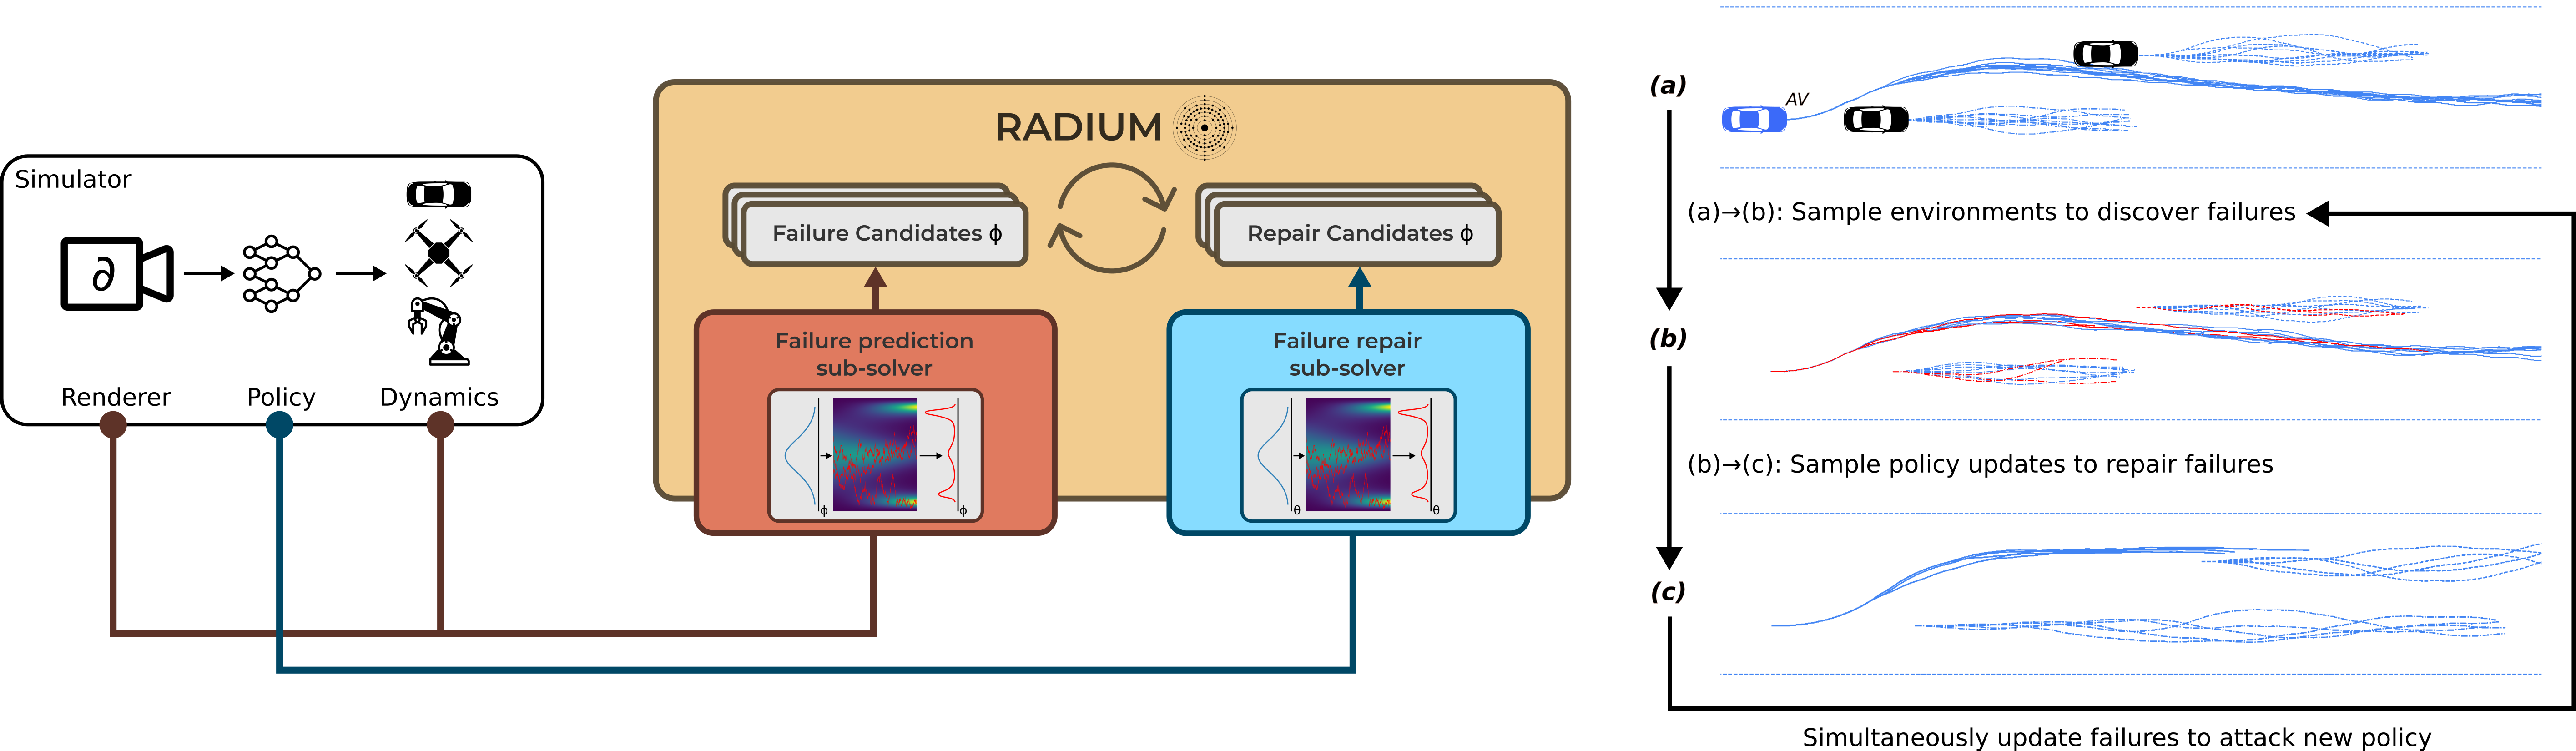
\includegraphics[width=\linewidth]{images/corl/architecture.png}
    \caption{An overview of our approach for closed-loop rare-event prediction, which efficiently predicts and repairs failures in autonomous systems. Our framework alternates between failure prediction and repair sub-solvers, which use a simulated environment to efficiently sample from the distributions~\eqref{ch:corl:eq:failure_logprob_basic} and~\eqref{ch:corl:eq:repair_logprob_basic}. We use differentiable rendering and simulation to accelerate our method with end-to-end gradients, but we also propose a gradient-free implementation.}\label{ch:corl:fig:architecture}
\end{figure}

\paragraph{Challenge 1: Distribution shift during retraining} Previous methods have proposed generating failure examples for use in retraining, but there is an inherent risk of distribution shift when doing so. Once we repair the policy, previously-predicted failures become stale and are no longer useful for verification (i.e. the distribution of likely failures has shifted). In the worst case, this can lead to overconfidence if we claim to have repaired all previously-discovered failures while remaining vulnerable to other failures. To address this issue, we interleave failure and repair steps to continuously update the set of predicted failures as we repair the policy, creating an adversarial sampling process that generates a robust repaired policy along with a set of salient failure cases.

\paragraph{Challenge 2: Exploring diverse failure modes} Traditional methods like Markov chain Monte Carlo (MCMC) are able to sample from non-normalized likelihoods like~\eqref{ch:corl:eq:failure_logprob_basic} and \eqref{ch:corl:eq:repair_logprob_basic}, but they struggle to fully explore the search space when the likelihood is highly multi-modal. To mitigate this issue, we take inspiration from the recent success of diffusion processes \cite{songScoreBasedGenerativeModeling2023,zhongGuidedConditionalDiffusion2022} and sequential Monte Carlo algorithms \cite{rubinoIntroductionRareEvent2009a} that interpolate between an easy-to-sample prior distribution and a multi-modal target distribution. Instead of sampling directly from the posterior, we begin by sampling from the unimodal, easy-to-sample prior and then smoothly interpolate to the posterior distributions~\eqref{ch:corl:eq:failure_logprob_basic}-\eqref{ch:corl:eq:repair_logprob_basic}. This process yields the tempered likelihood functions:
%
\begin{align}
    \tilde{p}_{\rm{failure}} & \propto p_{\phi, 0}(\phi)e^{-\tau[J^* - J(\theta, \phi)]_+} \label{ch:corl:eq:failure_logprob_tempered}                                     \\
    %
    \tilde{p}_{\rm{repair}}  & \propto p_{\theta, 0}(\theta, \theta_0)e^{-\frac{\tau}{n}\sum_{\phi_i}[J(\theta, \phi_i)-J^*]_+} \label{ch:corl:eq:repair_logprob_tempered}
\end{align}
%
where the tempering parameter $\tau$ is smoothly varied from $0$ to $1$. When $\tau = 0$, this is equivalent to sampling from the prior distributions, and when $\tau \to 1$ we recover the full posteriors~\eqref{ch:corl:eq:failure_logprob_basic}-\eqref{ch:corl:eq:repair_logprob_basic}. This tempering process reduces the risk of overfitting to one particular mode of the failure distribution and encourages even exploration of the failure space.

\paragraph{Challenge 3: Efficiently sampling in high dimension}
%
Previous works have proposed a wide variety of sampling algorithms that might be used as sub-solvers in our framework, including MCMC methods like random-walk Metropolis-Hastings (RMH;~\cite{hastingsMonteCarloSampling1970}), Hamiltonian Monte Carlo (HMC;~\cite{nealMCMCUsingHamiltonian2011}), and the Metropolis-adjusted Langevin algorithm (MALA;~\cite{julianbresagCommentsGrenadierMiller1994}), variational inference methods like Stein Variational Gradient Descent (SVGD;~\cite{liuSteinVariationalGradient2016a}), and other black-box methods like adaptive importance sampling~\cite{okellyScalableEndtoEndAutonomous2018}. RADIUM is able to use any of these sampling methods as sub-solvers for either prediction or repair. Generally, these sampling methods can be classified as either gradient-free or gradient-based. Theoretical and empirical evidence suggests that gradient-based methods can enjoy faster mixing time in high dimensions on certain classes of sufficiently smooth non-convex problems~\cite{maSamplingCanBe2019}, but autonomous systems with visual feedback have historically  been treated as black-boxes due to an inability to backpropagate through the rendering step \cite{zhouRoCUSRobotController2021,okellyScalableEndtoEndAutonomous2018,sinhaNeuralBridgeSampling2020}.
%
To enable the use of gradient-based samplers in RADIUM, we draw upon recent advances in differentiable simulation and rendering~\cite{huDiffTaichiDifferentiableProgramming2019,lelidecDifferentiableRenderingPerturbed2021} provide end-to-end gradients. In Sections~\ref{ch:corl:theory} and~\ref{ch:corl:experiments}, we provide theoretical and empirical evidence of a performance advantage for gradient-based samplers, but in order to make RADIUM compatible with existing non-differentiable simulators we also conduct experiments using gradient-free sampling subroutines.

\subsection{RADIUM}

Pseudocode for RADIUM is provided in Algorithm~\ref{ch:corl:alg:adv_diffusion}. The algorithm maintains a population of candidate repaired policies $[\theta_1, \ldots, \theta_n]$ and failures $[\phi_1, \ldots, \phi_n]$ that are updated over $N$ sampling rounds. In each round, we sample a set of new candidate policies from the repair pseudo-posterior~\eqref{ch:corl:eq:repair_logprob_tempered}, then sample a new set of failures that attack the current population of policies. In practice, we average the tempered failure log probability~\eqref{ch:corl:eq:failure_logprob_tempered} over the population of candidate designs, which results in a smoother distribution.

RADIUM supports a wide range of subroutines for sampling candidate failures and repaired policies. In our experiments, we include RMH and MALA (gradient-free and gradient-based MCMC algorithms, respectively). We choose these particular methods to provide a direct comparison between similar algorithms with and without gradients, as MALA reduces to RMH when the gradient is zero. Pseudocode for MALA is included in Algorithm~\ref{ch:corl:alg:mala}.

A final practical consideration is that although the stochasticity in our sampling-based approach can help us explore the design and failure spaces, we incur a degree of sub-optimality as a result. When using gradient-based sampling, we have the option to reduce this sub-optimality by ``quenching'' the solution: switching to simple gradient descent (e.g. using MALA for the first 90 rounds and then gradient descent on the last 10 rounds). In practice, we find that quenching can noticeably improve the final cost without compromising the diversity of predicted failure modes. Quenching is particularly important on problems where the cost function includes penalty terms for constraint satisfaction, where a few rounds of gradient descent can help to satisfy these constraints.

\begin{algorithm}
    \SetAlgoLined
    \SetKwInput{Input}{Input}
    \SetKwInput{Return}{Return}
    \Input{$N$ rounds, $K$ steps per round, stepsize $\lambda$, population size $n$, tempering rate $\alpha$, sampling algorithm (e.g. MALA as in Alg.~\ref{ch:corl:alg:mala})}

    Sample initial failures and policies using priors: $[\phi_1, \ldots, \phi_n]_0 \overset{\mathrm{iid}}{\sim} p_{\phi, 0},\ [\theta_1, \ldots, \theta_n]_0 \overset{\mathrm{iid}}{\sim} p_{\theta, 0}$\;

    \For{$i = 1, \ldots, N$}{
        $\tau \gets 1 - e^{-\alpha i / N}$\tcp*{Tempering schedule}
        %
        Sample $[\theta_1, \ldots, \theta_n]_i \overset{\mathrm{iid}}{\sim}$ \eqref{ch:corl:eq:repair_logprob_tempered}\tcp*{Sample repaired policies}\label{ch:corl:line:policy_update1}
        %
        % ${\theta_i}^* \gets \overset{\phantom{iid}}{\argmax_i} $ \eqref{ch:corl:eq:repair_logprob_tempered}\tcp*{Choose new best policy}\label{ch:corl:line:policy_update2}
        %
        Sample $[\phi_1, \ldots, \phi_n]_i \overset{\mathrm{iid}}{\sim}$ \eqref{ch:corl:eq:failure_logprob_tempered}\tcp*{Generate failures attacking $\theta^*_i$}\label{ch:corl:line:env_update}
    }

    \Return{Repaired policy $\theta^*_N = \argmax_i$ \eqref{ch:corl:eq:repair_logprob_tempered} and failures $[\phi_1, \ldots, \phi_n]_N$ attacking that policy.}

    \caption{RADIUM: Robustness via Adversarial Diversity Using MCMC}\label{ch:corl:alg:adv_diffusion}
\end{algorithm}

\subsection{Theoretical analysis}\label{ch:corl:theory}

The iterative adversarial sampling process defined in Alg.~\ref{ch:corl:alg:adv_diffusion} raises a few theoretical questions. First, when can we expect the individual sampling steps on lines~\ref{ch:corl:line:policy_update1} and~\ref{ch:corl:line:env_update} to converge, and under what conditions might we expect a gradient-based sampling sub-routine to converge faster than a gradient-free one? Second, assuming that these individual samplers converge, what sort of policies will result from the adversarial sampling loop in Alg.~\ref{ch:corl:alg:adv_diffusion}?

\paragraph{Convergence and gradient acceleration}
RADIUM inherits the asymptotic convergence guarantees of the particular subsolvers used for each sampling step. For example, when using an MCMC sampler, so long as that sampler can propose arbitrarily large steps with non-zero probability and satisfies the detailed balance condition (e.g. through the use of a Metropolis adjustment), then the sampler will produce samples asymptotically close to the target sampling distribution. Since the conditions for asymptotic convergence of MCMC samplers are relatively weak~\cite{hastingsMonteCarloSampling1970}, it is more interesting to ask about finite-sample convergence rates; in particular, under what conditions can we expect gradient-based samplers like MALA to accelerate convergence to the target distribution?

In many robotics problems, even when analytical gradients are available, it is unclear whether these gradients are useful for optimization (i.e. low empirical bias and variance;~\cite{suhDifferentiableSimulatorsGive2022}). Here, we build on recent theoretical results by~\cite{maSamplingCanBe2019} to provide sufficient conditions for fast, polynomial-time convergence of gradient-based samplers in our setting. With slight abuse of notation, we use $J(\theta, \phi)$ to denote the composition of the simulator and cost function.

\begin{theorem}\label{ch:corl:thm:convergence}
    Let $J(\theta, \phi)$ be a $L$-Lipschitz smooth cost function (i.e. $\nabla J$ is $L$-Lipschitz continuous), let the log prior distributions $\log p_{\phi ,0}$ and $\log p_{\theta,0}$ be Lipschitz smooth everywhere and $m$-strongly convex outside a ball of finite radius $R$, and let $d = \max\pn{\dim{\theta}, \dim{\phi}}$ be the dimension of the search space. If $m > L$, then MALA with appropriate step size will yield samples within $\epsilon$ total variation distance of the target distributions~\eqref{ch:corl:eq:failure_logprob_tempered} and~\eqref{ch:corl:eq:repair_logprob_tempered} with total number of sampling steps $\leq \widetilde{\mathcal{O}}\pn{d^2 \ln\frac{1}{\epsilon}}$.
\end{theorem}

The key idea of the proof is to rely on the log-concavity of the prior distributions to dominate the non-convexity of the cost function sufficiently far from the central modes.

\begin{proof}
    We will show the proof for sampling from the failure generating process with likelihood given by Eq.~\eqref{ch:corl:eq:failure_logprob_tempered}; the proof for the repair generating process follows similarly. The log-likelihood for the failure generating process is
    \begin{equation}
        \log p_{\phi, 0}(\phi) - \tau [J^* - J(\theta, \phi)]_+ \label{ch:corl:eq:failure_logprob}
    \end{equation}

    \cite{maSamplingCanBe2019} show that MALA sampling enjoys the convergence guarantees of Theorem~\ref{ch:corl:thm:convergence} so long as the target log likelihood is strongly convex outside of a ball of finite radius $R$ (see Theorem 1 in \cite{maSamplingCanBe2019}). Since $\log p_{\phi, 0}(\phi)$ is assumed to be strongly $m$-convex, it is sufficient to show that as $||\phi|| \to \infty$, the strong convexity of the log-prior dominates the non-convexity in $\tau [J^* - J(\theta, \phi)]_+$.

    For convenience, denote $f(\phi) = -\tau [J^* - J(\theta, \phi)]_+$ and $g(\phi) = \log p_{\phi, 0}(\phi)$. We must first show that $f(\phi) + g(\phi)$ is $(m-L)$-strongly convex, for which it suffices to show that $f(\phi) + g(\phi) - (m-L)/2 ||\phi||^2$ is convex. Note that
    \begin{align}
        f(\phi) + g(\phi) - \frac{m-L}{2} ||\phi||^2 & = f(\phi) + \frac{L}{2} ||\phi||^2 + g(\phi) - \frac{m}{2} ||\phi||^2
    \end{align}
    $g(\phi) - \frac{m}{2} ||\phi||^2$ is convex by $m$-strong convexity of $g$, so we must show that the remaining term, $f(\phi) + L/2 ||\phi||^2$, is convex. Note that the Hessian of this term is $\nabla^2 f(\phi) + LI$. Since we have assumed that $J$ is $L$-Lipschitz smooth (i.e. its gradients are $L$-Lipschitz continuous), it follows that the magnitudes of the eigenvalues of $\nabla^2 f$ are bounded by $L$, which is sufficient for $\nabla^2 f(\phi) + LI$ to be positive semi-definite, completing the proof.
\end{proof}

Theorem~\ref{ch:corl:thm:convergence} requires smoothness assumptions on the cost; we recognize that this assumption is difficult to verify in practice and does not hold in certain domains (notably when rigid body contact is involved). However, in the problems we consider it is possible to smooth the simulator (e.g. using smoothed dynamics and a blurred renderer and scene representation), thus smoothing the gradients of $J$. The smoothness and convexity conditions hold for many common prior distributions, such as Gaussian and smoothed uniform distributions.

\paragraph{Adversarial Joint Distribution} Even if the samplers for both policy and environmental parameters converge within each round of Alg.~\ref{ch:corl:alg:adv_diffusion}, it is not clear what will be the effect of running these samplers repeatedly in an adversarial manner. Our next theoretical result defines the joint distribution of $\theta$ and $\phi$ as a result of this adversarial sampling loop. To simplify the theoretical analysis, we consider the case when population size $n=1$, and we replace the smooth ELU with a ReLU in~\eqref{ch:corl:eq:failure_logprob_basic} and~\eqref{ch:corl:eq:repair_logprob_basic}.

\begin{theorem}\label{ch:corl:thm:joint}
    The iterative adversarial sampling procedure in Alg.~\ref{ch:corl:alg:adv_diffusion} yields policies drawn from a marginal distribution with unnormalized density function
    \begin{equation}
        f_\theta(\theta^*) = p_{\theta, 0}(\theta^*) \pn{\frac{\expectation_{\phi \sim p_{\phi, 0}}\left[ e^{J(\theta^*, \phi) - J^*} | J(\theta^*, \phi) \leq J^* \right]}{\expectation_{\phi \sim p_{\phi, 0}}\left[ e^{J(\theta^*, \phi) - J^*} \right]} +
            %
            \frac{\mathbb{P}[J(\theta^*, \phi) > J^*]}{\expectation_{\phi \sim p_{\phi, 0}}\left[ e^{J(\theta^*, \phi) - J^*}\right]}}\label{ch:corl:eq:marginal}
    \end{equation}
    where $\mathbb{P}(J(\theta^*, \phi) > J^* = \expectation_{\phi \sim p_{\phi, 0}}[\mathbbm{1}(J(\theta^*, \phi) \geq J^*)]$ is the probability of failure when $\phi$ is sampled from the prior distribution.
\end{theorem}

The first term in the parenthesis in~\eqref{ch:corl:eq:marginal} is bounded above by $1$ and maximized when the policy does not experience failure (in which case the conditional and unconditional expectations will be equal). The numerator of the second term bounded $[0, 1]$, while the denominator grows exponentially large when a failure occurs. As a result, the marginal distribution of $\theta^*$ assigns higher probability (relative to the prior) for policies that avoid failure.

\begin{proof}
    We can treat Alg.~\ref{ch:corl:alg:adv_diffusion} as a two-stage Gibbs sampling procedure and apply the Hammersley-Clifford Theorem~\cite{robertMonteCarloStatistical2004} to get the joint distribution
    \begin{equation}
        f_{\theta, \phi}(\theta^*, \phi^*) = p_{\theta, 0}(\theta^*) p_{\phi, 0}(\phi^*) \frac{e^{-[J^* - J(\theta^*, \phi^*)]_+}}{\expectation_{\phi \sim p_{\phi, 0}}\left[ e^{J(\theta^*, \phi) - J^*} \right]} \label{ch:corl:eq:joint}
    \end{equation}

    Integrating over $\phi$ yields the marginal distribution of $\theta$, completing the proof.
    \begin{align}
        f_{\theta^*} & = \int_\phi f_{\theta, \phi}(\theta^*, \phi) d\phi = \frac{p_{\theta, 0}(\theta^*)}{\expectation_{\phi \sim p_{\phi, 0}}\left[ e^{J(\theta^*, \phi) - J^*} \right]}  \int_\phi p_{\phi, 0}(\phi) e^{-[J^* - J(\theta^*, \phi^*)]_+} d\phi                                                                               \\
        %
                     & = p_{\theta, 0}(\theta^*)\frac{\expectation_{\phi \sim p_{\phi, 0}}\left[ e^{-[J^* - J(\theta^*, \phi)]_+} \right]}{\expectation_{\phi \sim p_{\phi, 0}}\left[ e^{J(\theta^*, \phi) - J^*} \right]}                                                                                                                     \\
        %
                     & = p_{\theta, 0}(\theta^*)\frac{\expectation_{\phi \sim p_{\phi, 0}}\left[ e^{-(J^* - J(\theta^*, \phi))} | J^* - J(\theta^*, \phi) \geq 0 \right] + \expectation_{\phi \sim p_{\phi, 0}}\left[ 1 | J^* - J(\theta^*, \phi) < 0 \right]}{\expectation_{\phi \sim p_{\phi, 0}}\left[ e^{J(\theta^*, \phi) - J^*} \right]} \\
        %
                     & = p_{\theta, 0}(\theta^*)\frac{\expectation_{\phi \sim p_{\phi, 0}}\left[ e^{-(J^* - J(\theta^*, \phi))} | J^* \geq J(\theta^*, \phi) \right] + \expectation_{\phi \sim p_{\phi, 0}}\left[ 1 | J^* < J(\theta^*, \phi) \right]}{\expectation_{\phi \sim p_{\phi, 0}}\left[ e^{J(\theta^*, \phi) - J^*} \right]}         \\
                     & = p_{\theta, 0}(\theta^*)\frac{\expectation_{\phi \sim p_{\phi, 0}}\left[ e^{-(J^* - J(\theta^*, \phi))} | J^* \geq J(\theta^*, \phi) \right] + \mathbb{P}[J(\theta^*, \phi) > J^*]}{\expectation_{\phi \sim p_{\phi, 0}}\left[ e^{J(\theta^*, \phi) - J^*} \right]}                                                    \\
    \end{align}
\end{proof}

\section{Simulation experiments}\label{ch:corl:experiments}

In this section, we provide empirical comparisons of RADIUM with existing methods for adversarial optimization and policy repair in a range of simulated environments. We have two main goals in this section. First, we seek to understand whether re-framing the failure repair problem from optimization to inference leads to better solutions (i.e. more robust designs and better coverage by the predicted failures). Second, we study whether the gradient-based version of our method yields any benefits over the gradient-free version. After the empirical comparisons in this section, Section~\ref{ch:corl:case_studies} then provides three case studies with a more in-depth discussion of how RADIUM can be applied to practical verification and design problems, including two case studies demonstrating how repaired designs can be transferred from simulation to hardware.

We conduct simulation studies on a range of problems from the robotics and cyberphysical systems literature, comparing against previously-published adversarial optimization methods. More detail on each benchmark, baseline, and implementation is provided in the appendix.

\subsection{Experimental setup}

\subsubsection{Baselines}

We compare with three baselines taken from the adversarial optimization and testing literature.
%
\textit{Gradient descent with randomized counterexamples (\gdr)} optimizes the design using a fixed set of random counterexamples, representing a generic policy optimization with domain randomization approach.
%
\textit{Gradient descent with adversarial counterexamples (\gda)} alternates between optimizing the design and optimizing for maximally adversarial failure modes, as in~\cite{hanselmannKINGGeneratingSafetyCritical2022a,dawsonRobustCounterexampleguidedOptimization2022b}.
%
\textit{Learning to collide (\ltc)} uses black-box optimization (REINFORCE) to search for failure cases~\cite{dingLearningCollideAdaptive2020a}.
%
We denote the gradient-free and gradient-based variants of RADIUM as $R_0$ and $R_1$, respectively.
%
All methods were run on the same GPU model with the same number of rounds for each task. Hyperparameters for all experiments are given in the appendix.

\subsubsection{Benchmark problems}

We rely on two classes of benchmark problem in this work: three problems without vision in the loop, and four problems with vision in the loop. Some of these problem domains include multiple environments of varying complexity, for a total of 13 different environments. A summary of these environments is given in Fig~\ref{ch:corl:fig:environments}. More details on the parameters and cost functions used for each environment are given in the appendix.

\begin{figure*}[t]
    \centering
    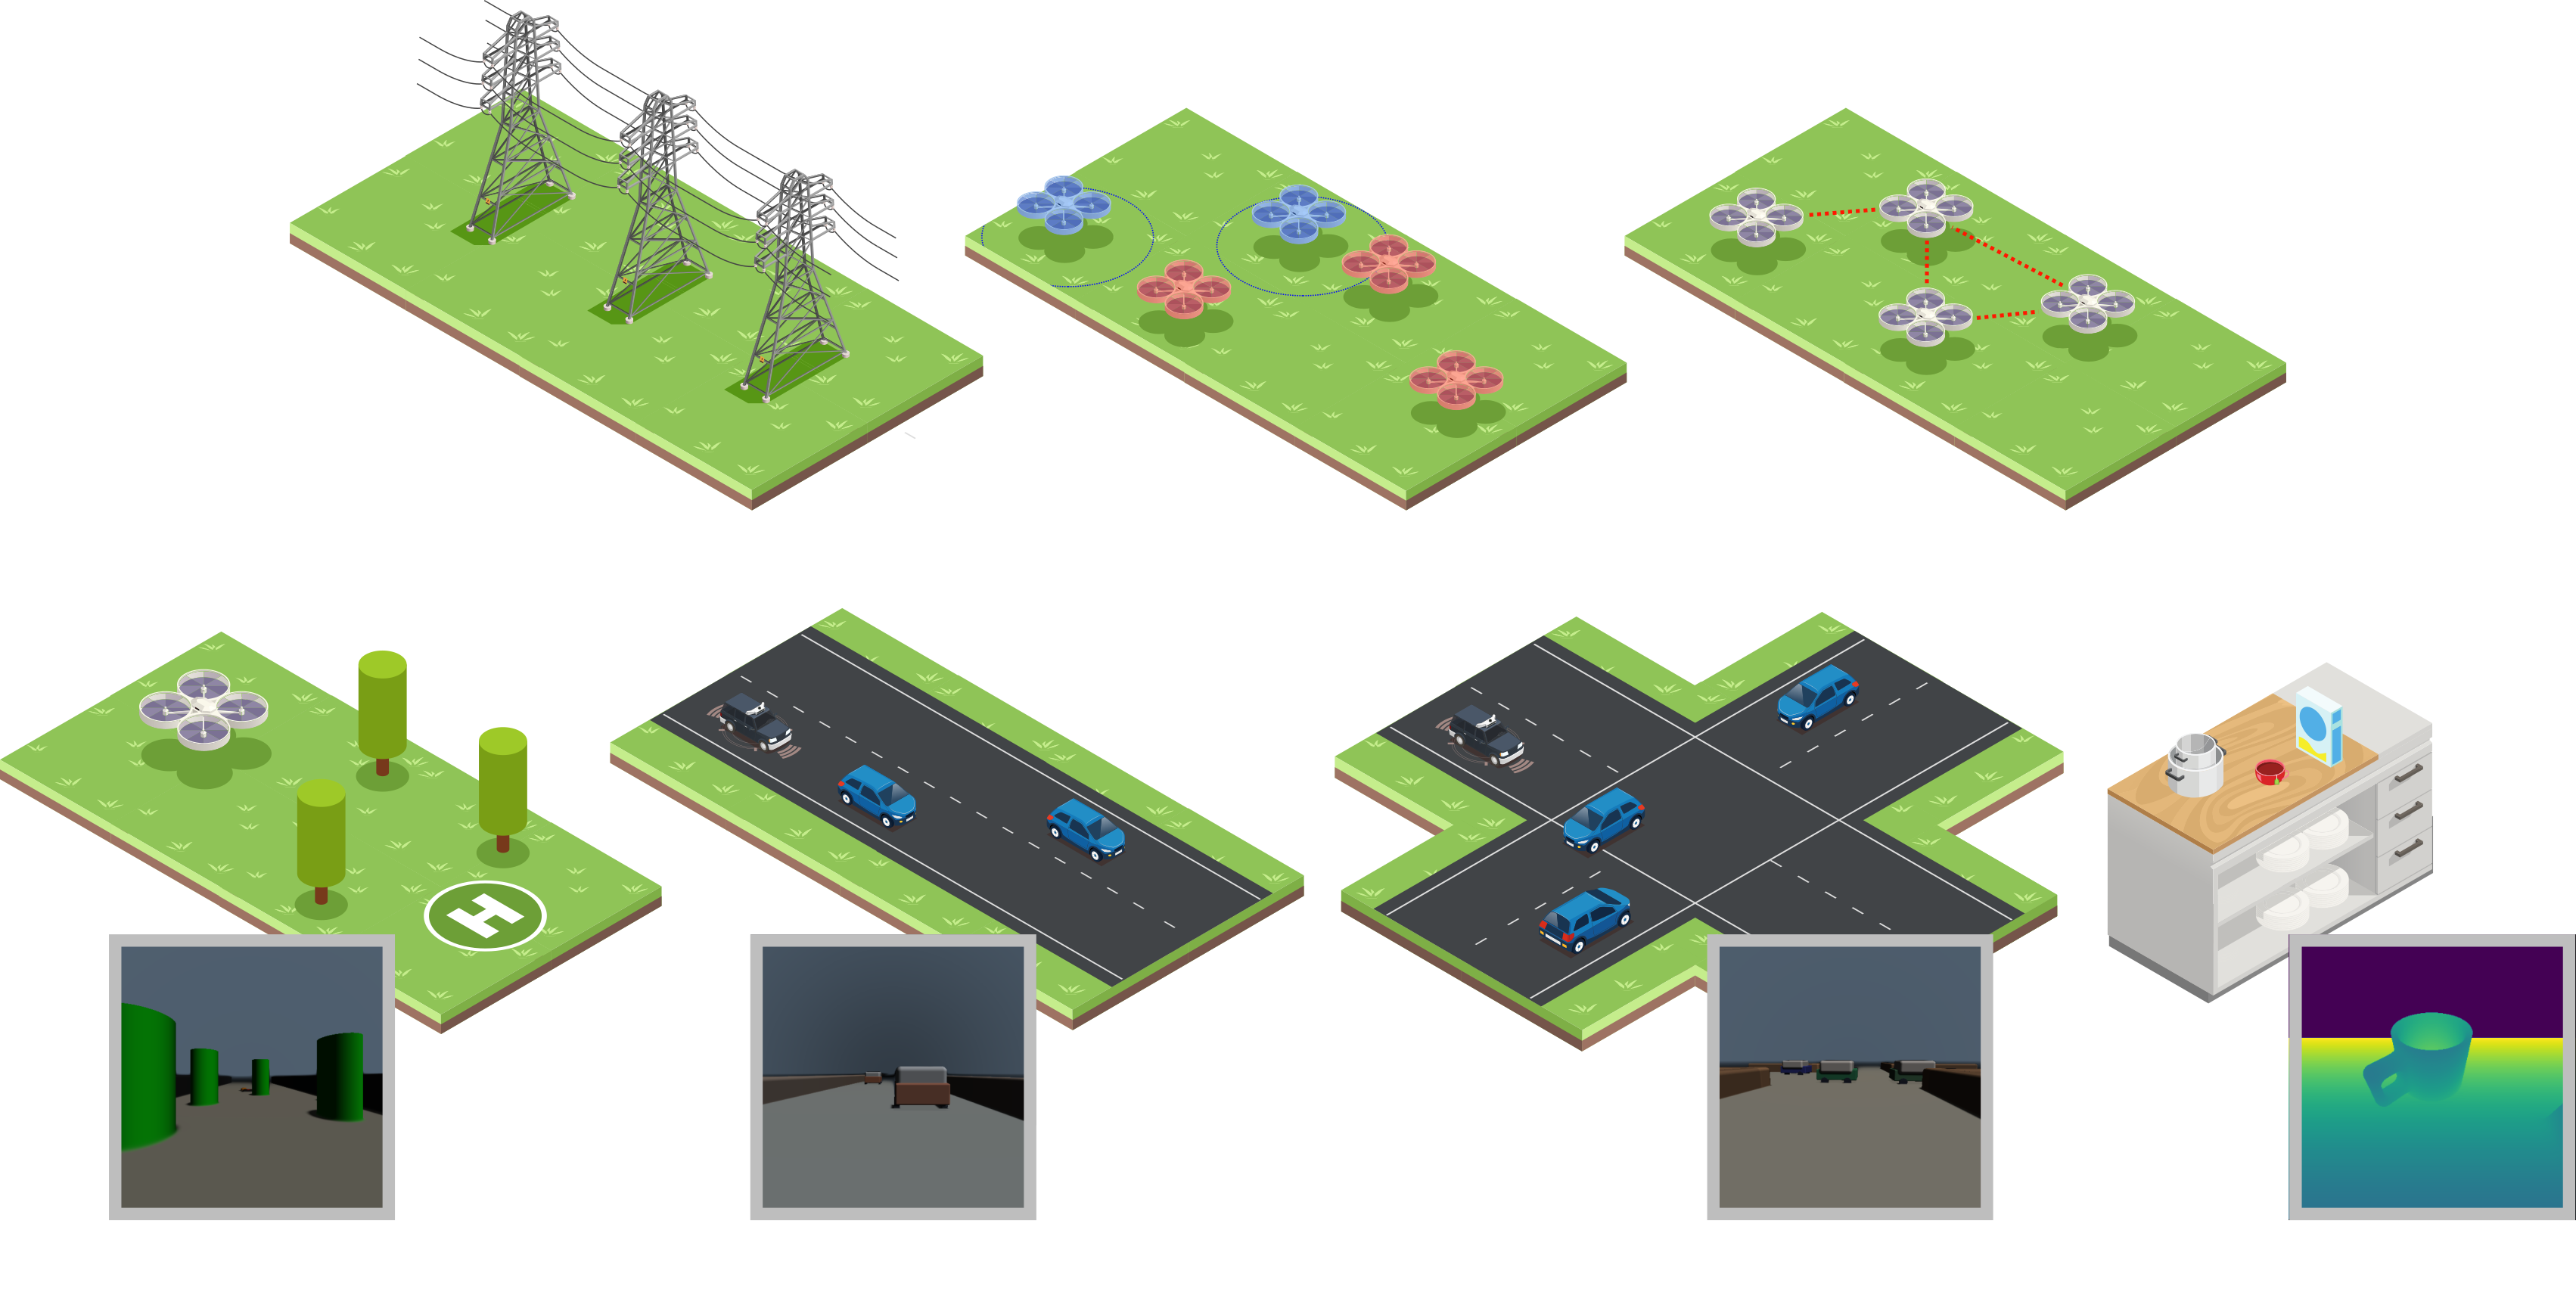
\includegraphics[width=\linewidth]{images/corl/all_examples.png}
    \caption{The different environments used in our simulation studies, including 3 domains without visual feedback (power grid, search, and formation control) and 4 domains with vision in the loop (drone, AV highway, AV intersection, and grasping). The inset shows the robot's perspective in the vision-in-the-loop tasks.}\label{ch:corl:fig:environments}
\end{figure*}

\paragraph{Non-vision benchmarks}
%
\textit{Search:} a set of seeker robots must cover a region to detect a set of hiders. $\theta$ and $\phi$ define trajectories for the seekers and hiders, respectively. Failure occurs if any hider escapes detection by the seekers (which have fixed sensing radius). This environment has two variants: small (6 seeker vs. 10 hider, $\dim{\theta} = 60$, $\dim{\phi} = 100$) and large (12 seeker vs. 20 hider, $\dim{\theta} = 120$, $\dim{\phi} = 200$).
%
\textit{Formation control:} a swarm of drones fly to a goal while maintaining full connectivity with a limited communication radius. $\theta$ defines trajectories for each robot in the swarm, while $\phi$ defines an uncertain wind velocity field. Failure occurs when the second eigenvalue of the graph Laplacian is close to zero. This environment has small (5 agent, $\dim{\theta} = 30$, $\dim{\phi} = 4$) and large (10 agent, $\dim{\theta} = 100$, $\dim{\phi} = 4$) variants.
%
\textit{Power grid dispatch:} electric generators must be scheduled to ensure that the network satisfies voltage and maximum power constraints in the event of transmission line outages. $\theta$ specifies generator setpoints and $\phi$ specifies line admittances; failures occur when any of the voltage or power constraints are violated. This environment has small (14-bus, $\dim{\theta} = 32$, $\dim{\phi} = 20$) and large (57-bus, $\dim{\theta} = 98$, $\dim{\phi} = 80$) versions.
% %
% \textit{GCAS:} a ground collision avoidance system (GCAS) must be designed to prevent a jet aircraft, modeled with aerodynamic effects and engine dynamics, from crashing into the ground. $\theta$ defines a control policy neural network ($\dim{\theta}\approx 1.8\times10^3$) and $\phi$ defines the initial conditions ($\dim{\phi} = 5$).
% %
% \textit{Pushing:} a robot manipulator must push an object out of the way to reach another object. Failure occurs if the object is knocked over while pushing. $\theta$ defines a planning policy network ($\dim{\theta} \approx 1.2\times10^3$) and $\phi$ defines the unknown inertial and frictional properties of the object being pushed, as well as measurement noises ($\dim{\phi} = 7$).

\paragraph{Vision-in-the-loop benchmarks}

\textit{AV (highway):} An autonomous vehicle must overtake two other vehicles.
%
\textit{AV (intersection):} the autonomous vehicle must navigate an uncontrolled intersection with crossing traffic.
%
In both AV tasks, the actions of the non-ego vehicles are uncertain, and the AV observes RGBd images from a front-facing camera as well as its own speed.
%
\textit{Drone:} A drone must safely navigate through a cluttered environment in windy conditions. There is uncertainty in the wind speed and location of all obstacles.
%  \textit{Drone (dynamic):} the same but the obstacles move with uncertain velocities.
%
Initial convolutional neural network (CNN) policies $\theta_0$ for drone and intersection environments were pre-trained using behavior cloning, and CNN-based policies for the highway environment were pre-trained using PPO~\cite{schulmanProximalPolicyOptimization2017}.
%
\textit{Grasp (box/mug): } a robot must locate and grasp an object using a depth image of the scene. There is uncertainty in the location of the objects and in the location of a nearby distractor object. The grasp detector is trained with labels of ground-truth grasp affordances.

The dimension of the failure space is 20 for the highway task, 30 for the intersection task, 12 for the drone task, and 4 for the grasping tasks. The dimension of the policy space is 64k for the highway and intersection tasks, 84k for the drone task, and 266k for the grasping tasks.

\subsubsection{Implementation}

Since we require a differentiable renderer and simulation engine for our work, we were not able to use an off-the-shelf simulator like CARLA~\cite{Dosovitskiy17}. Instead, we write our own simulator and basic differentiable renderer using JAX, which is available at \url{github.com/MIT-REALM/architect_corl_23}.
%
Likewise, our method and all baselines were implemented in JAX and compiled using JAX's just-in-time (JIT) compilation. Each metric reports the mean and standard deviation across four independent random seeds. All methods are given the same total sample budget for both prediction and repair (except for \gdr, which does not update the predicted failure modes).

The non-vision benchmarks were all initialized with random $\theta_0$, and the vision benchmarks were initialized using $\theta_0$ trained using reinforcement learning or behavior cloning with domain randomization. We include comparisons with \gdr, \gda, and \ltc{} on all non-vision benchmarks. Since $\theta_0$ on the vision benchmarks was trained using domain randomization, \gdr{} is not able to improve the initial parameters, and so we include comparisons with $\theta_0$, \gda, and \ltc{} for the vision benchmarks.

\subsubsection{Metrics}

To measure the robustness of the optimized policies, we report the failure rate (FR) on a test set of 1,000 i.i.d. samples of $\phi$ from the prior $p_{\phi, 0}$. We also report the mean cost on this test set as well as the maximum cost on the vision-in-the-loop benchmarks (where cost is bounded by construction) and the 99\textsuperscript{th}-percentile cost for non-vision benchmarks (some of which have unbounded cost, making the 99\textsuperscript{th} percentile more representative). Costs are normalized by the maximum cost observed across any method. Finally, for each task, we report the time required to run a simulation both with and without reverse-mode differentiation.

\subsection{Results}

Fig.~\ref{ch:corl:fig:nonvision_results} shows the results from benchmark problems without vision in the loop, while Fig.~\ref{ch:corl:fig:vision_results} shows the results from problems with vision in the loop. For ease of comparison, each plot groups the gradient-free methods (\ltc{} and $R_0$) and the gradient-based methods (\gdr, \gda, and $R_1$). Since the initial parameters for the vision-in-the-loop benchmarks in Fig.~\ref{ch:corl:fig:vision_results} were trained using RL or behavior cloning (which do not require differentiable simulation), we group $\theta_0$ with the gradient-free results in Fig.~\ref{ch:corl:fig:vision_results}. We also compare the convergence rates of each method in Fig.~\ref{ch:corl:fig:convergence}. Table~\ref{ch:corl:tab:runtime} shows the time required for simulating with and without automatic differentiation.

\begin{figure}[tb]
    \centering
    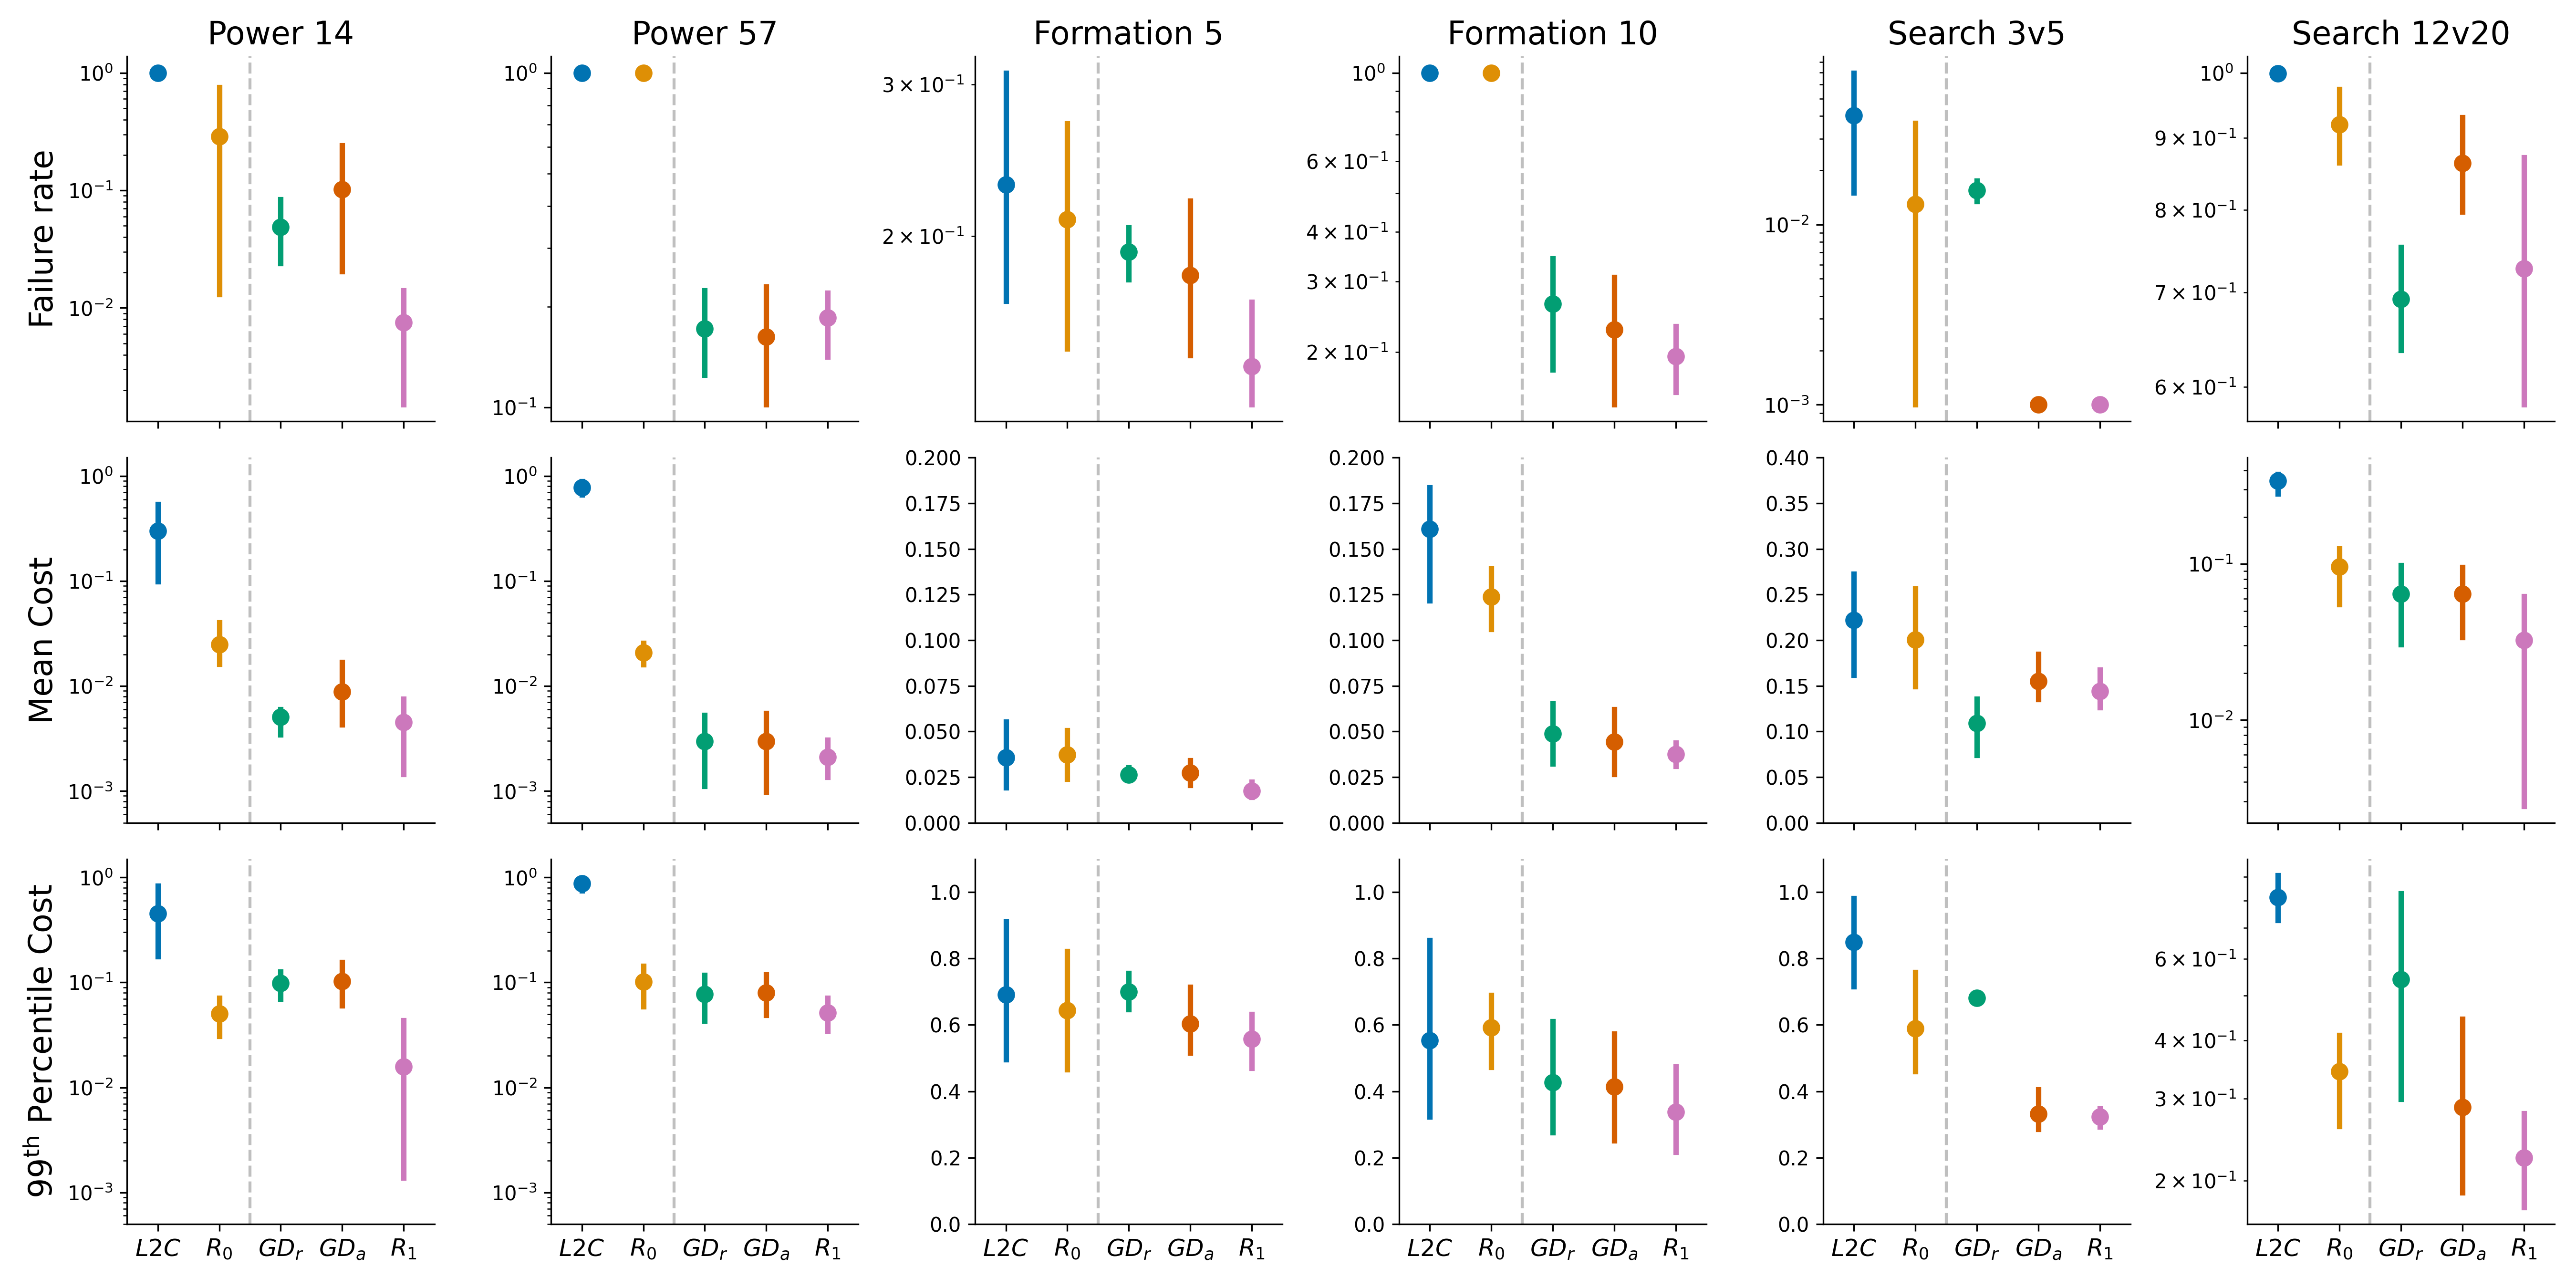
\includegraphics[width=\linewidth]{images/corl/nonvision.png}
    \caption{Comparison of our method (gradient-free and gradient-based variants $R_0$ and $R_1$, respectively) and baseline methods on benchmark problems without vision in the loop, showing failure rate, mean cost, and 99\textsuperscript{th} percentile cost on a test set of 1,000 randomly sampled $\phi$. The dashed gray lines separate gradient-free and gradient-based methods.}\label{ch:corl:fig:nonvision_results}
\end{figure}

\begin{figure}[tb]
    \centering
    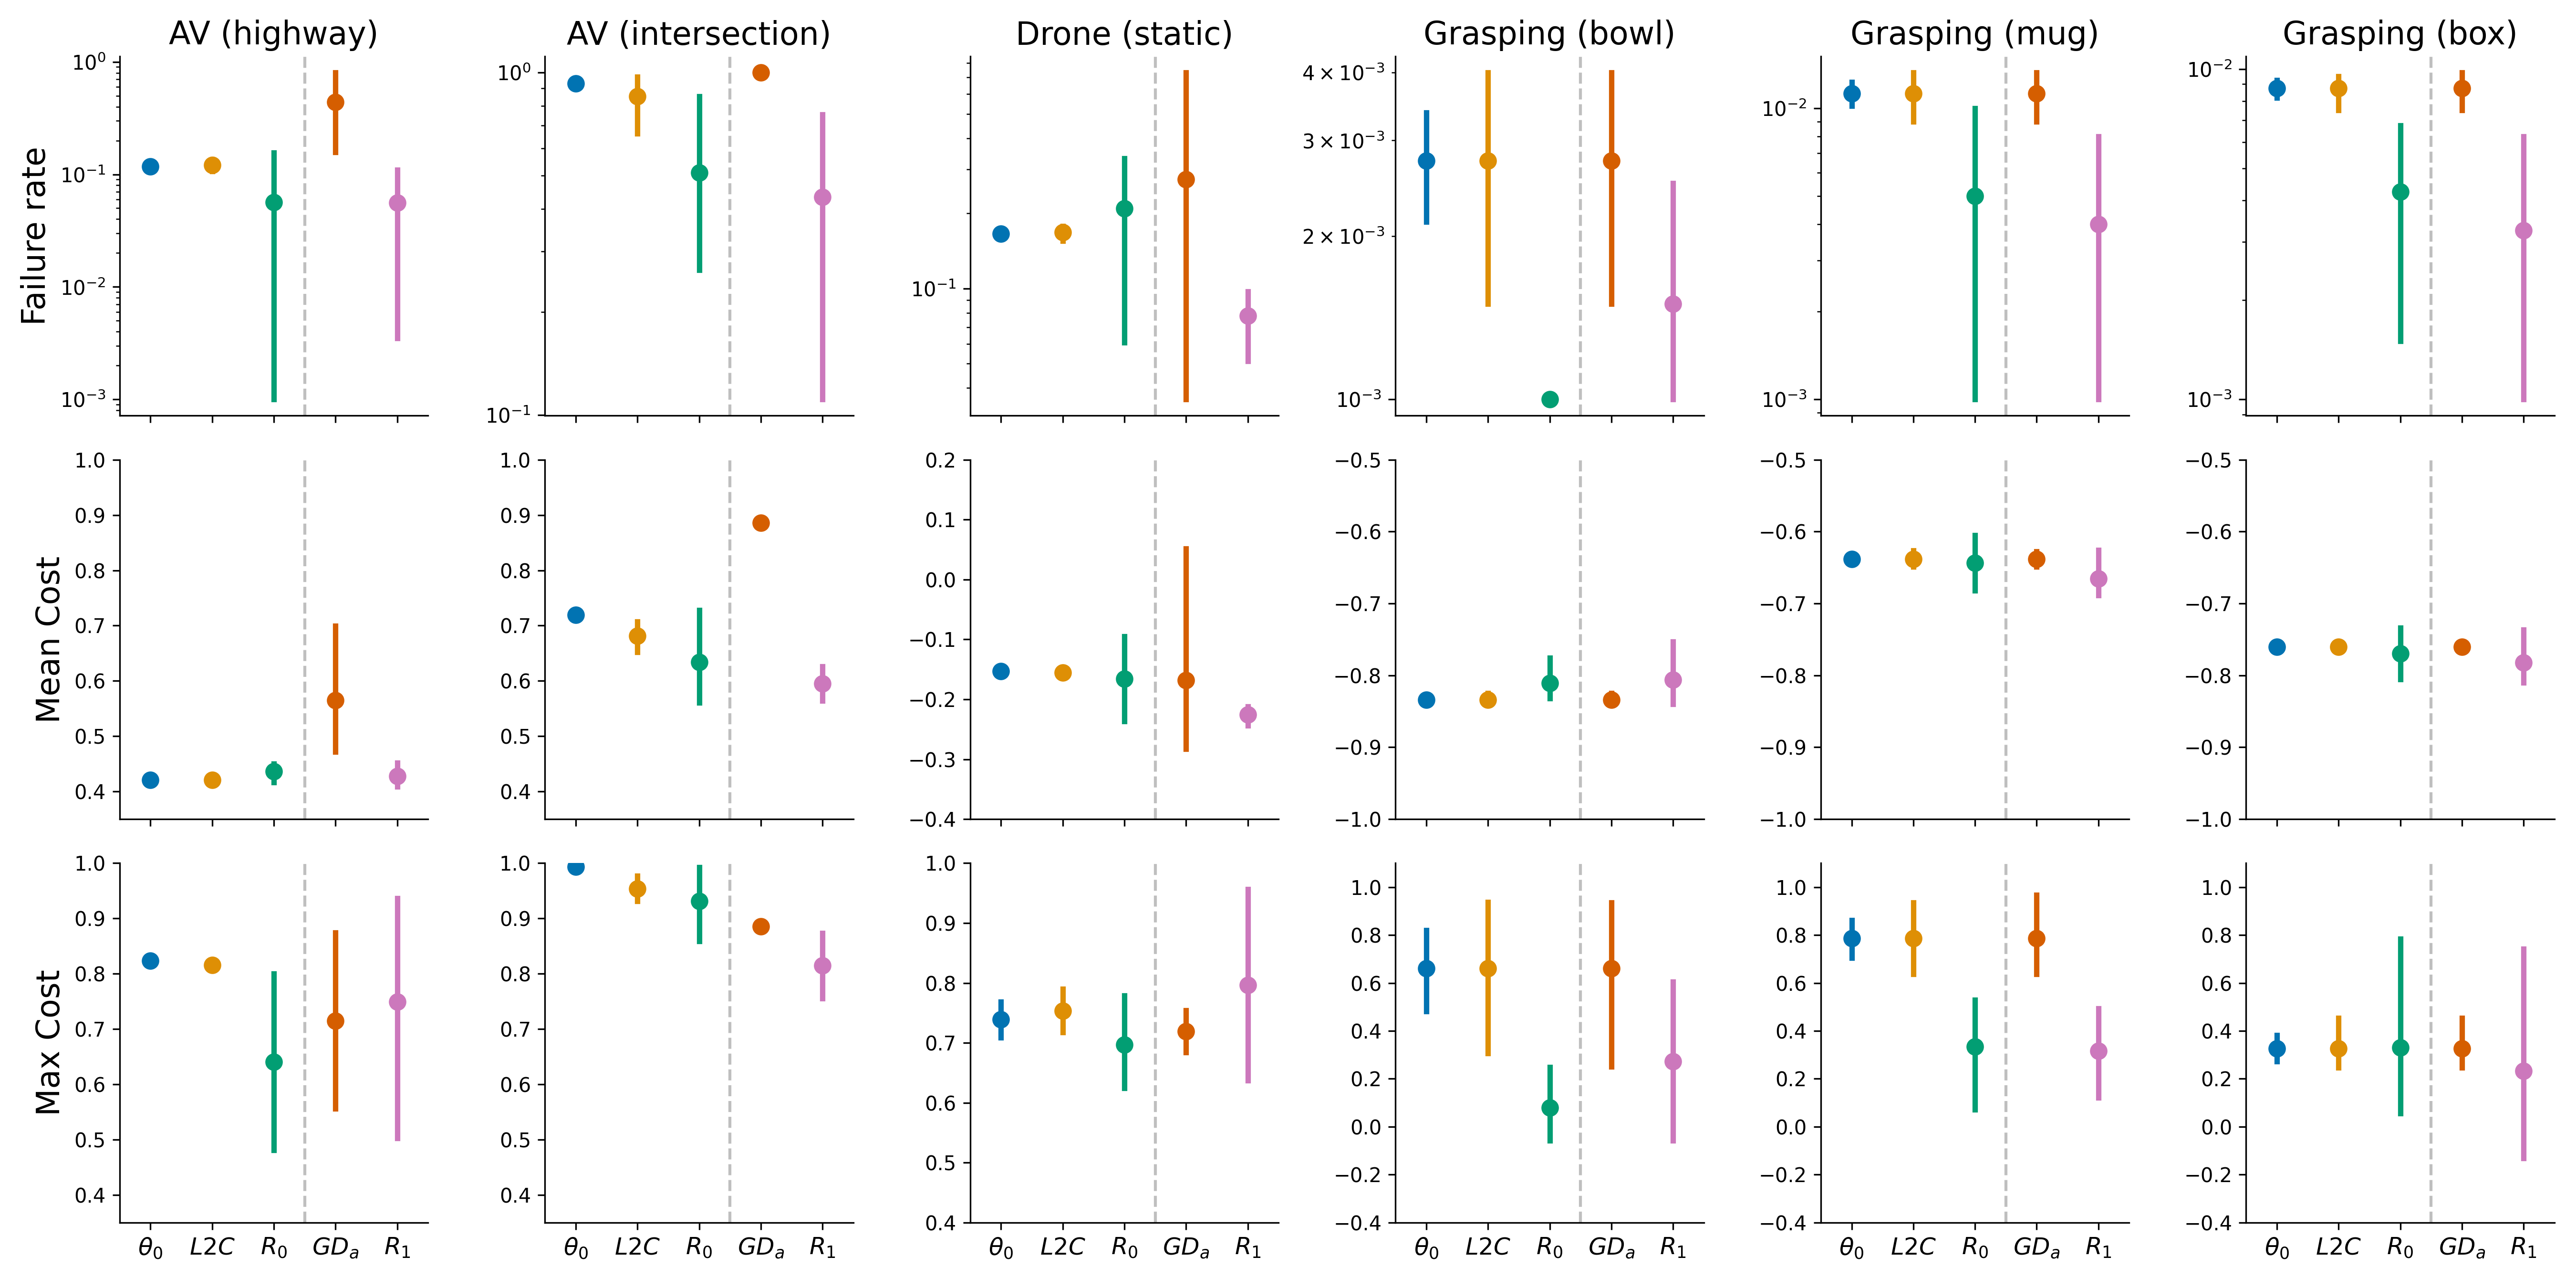
\includegraphics[width=\linewidth]{images/corl/vision.png}
    \caption{Comparison of our method (gradient-free and gradient-based variants $R_0$ and $R_1$, respectively) and baseline methods on benchmark problems with vision in the loop, showing failure rate, mean cost, and max cost on a test set of 1,000 randomly sampled $\phi$. The dashed gray lines separate gradient-free and gradient-based methods.}\label{ch:corl:fig:vision_results}
\end{figure}

\begin{figure}[tb]
    \centering
    \begin{subfigure}[t]{\linewidth}
        \centering
        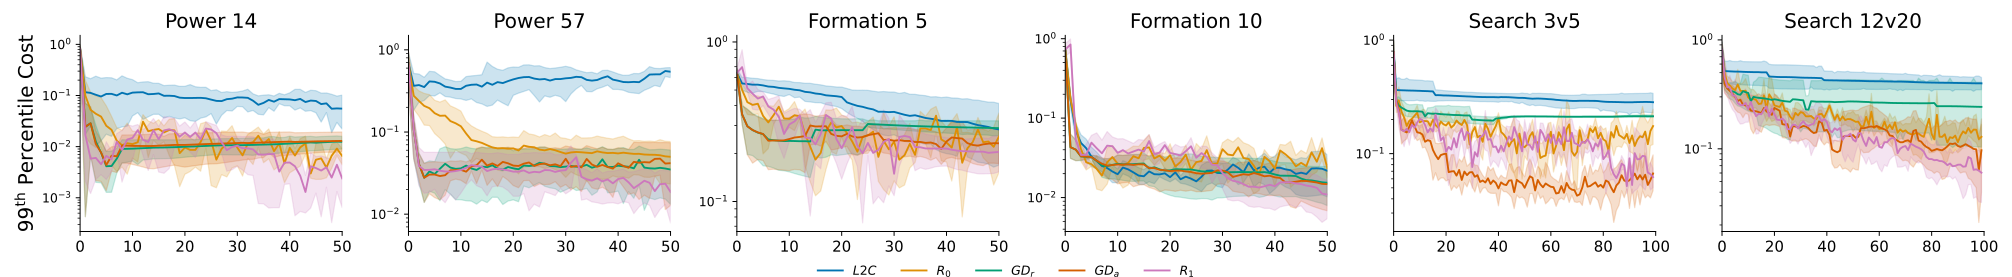
\includegraphics[width=\linewidth]{images/corl/nonvision_convergence.png}
        \caption{Non-vision benchmarks}\label{ch:corl:fig:convergence:nonvision}
    \end{subfigure}
    \begin{subfigure}[t]{\linewidth}
        \centering
        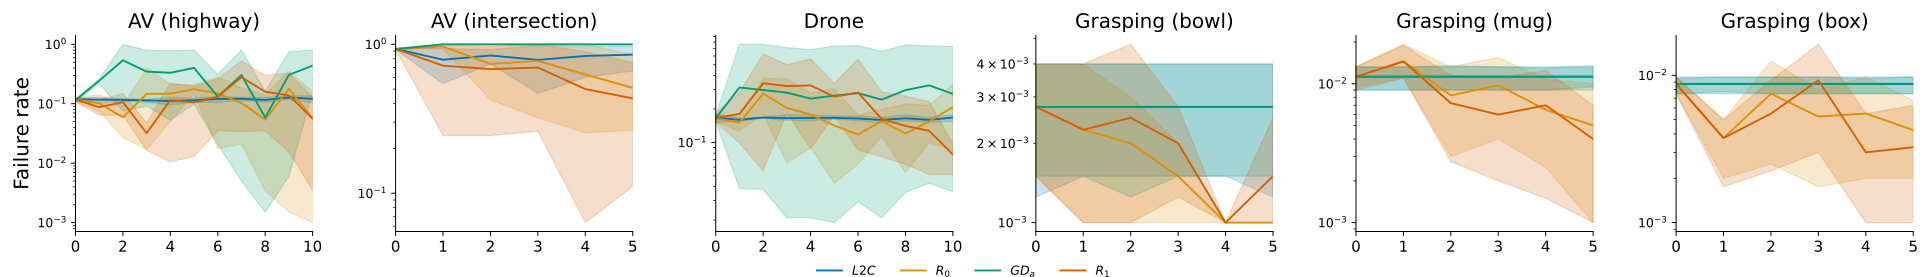
\includegraphics[width=\linewidth]{images/corl/vision_convergence.png}
        \caption{Vision-in-the-loop benchmarks}\label{ch:corl:fig:convergence:vision}
    \end{subfigure}
    \caption{Convergence rates of our method and baselines on tasks with (top) and without (bottom) vision in the loop.}\label{ch:corl:fig:convergence}
\end{figure}

Fig.~\ref{ch:corl:fig:repairs} shows examples of failure cases and repaired policies generated using $R_1$ on three vision-in-the-loop tasks: AV (highway), AV (intersection), and drone. The left of Fig.~\ref{ch:corl:fig:repairs} shows the initial policy $\theta_0$ and failure modes discovered using our method (sampling $\phi$ while holding $\theta_0$ fixed), while the right shows the repaired policy and updated challenging counterexamples. Since the distribution of failure modes shifts as we repair the policy, we continuously re-sample the failure modes to be relevant to the updated policy. In all cases, we see that the repaired policy found using our method experiences fewer failures, despite the updated adversarial failure modes. In certain cases, the repaired policy exhibits a qualitatively different behavior; for example, in the vision-in-the-loop highway control task, the repaired policy is less aggressive than the original policy, avoiding the risky overtake maneuver (top row of Fig.~\ref{ch:corl:fig:repairs}).

\begin{figure}[t]
    \centering
    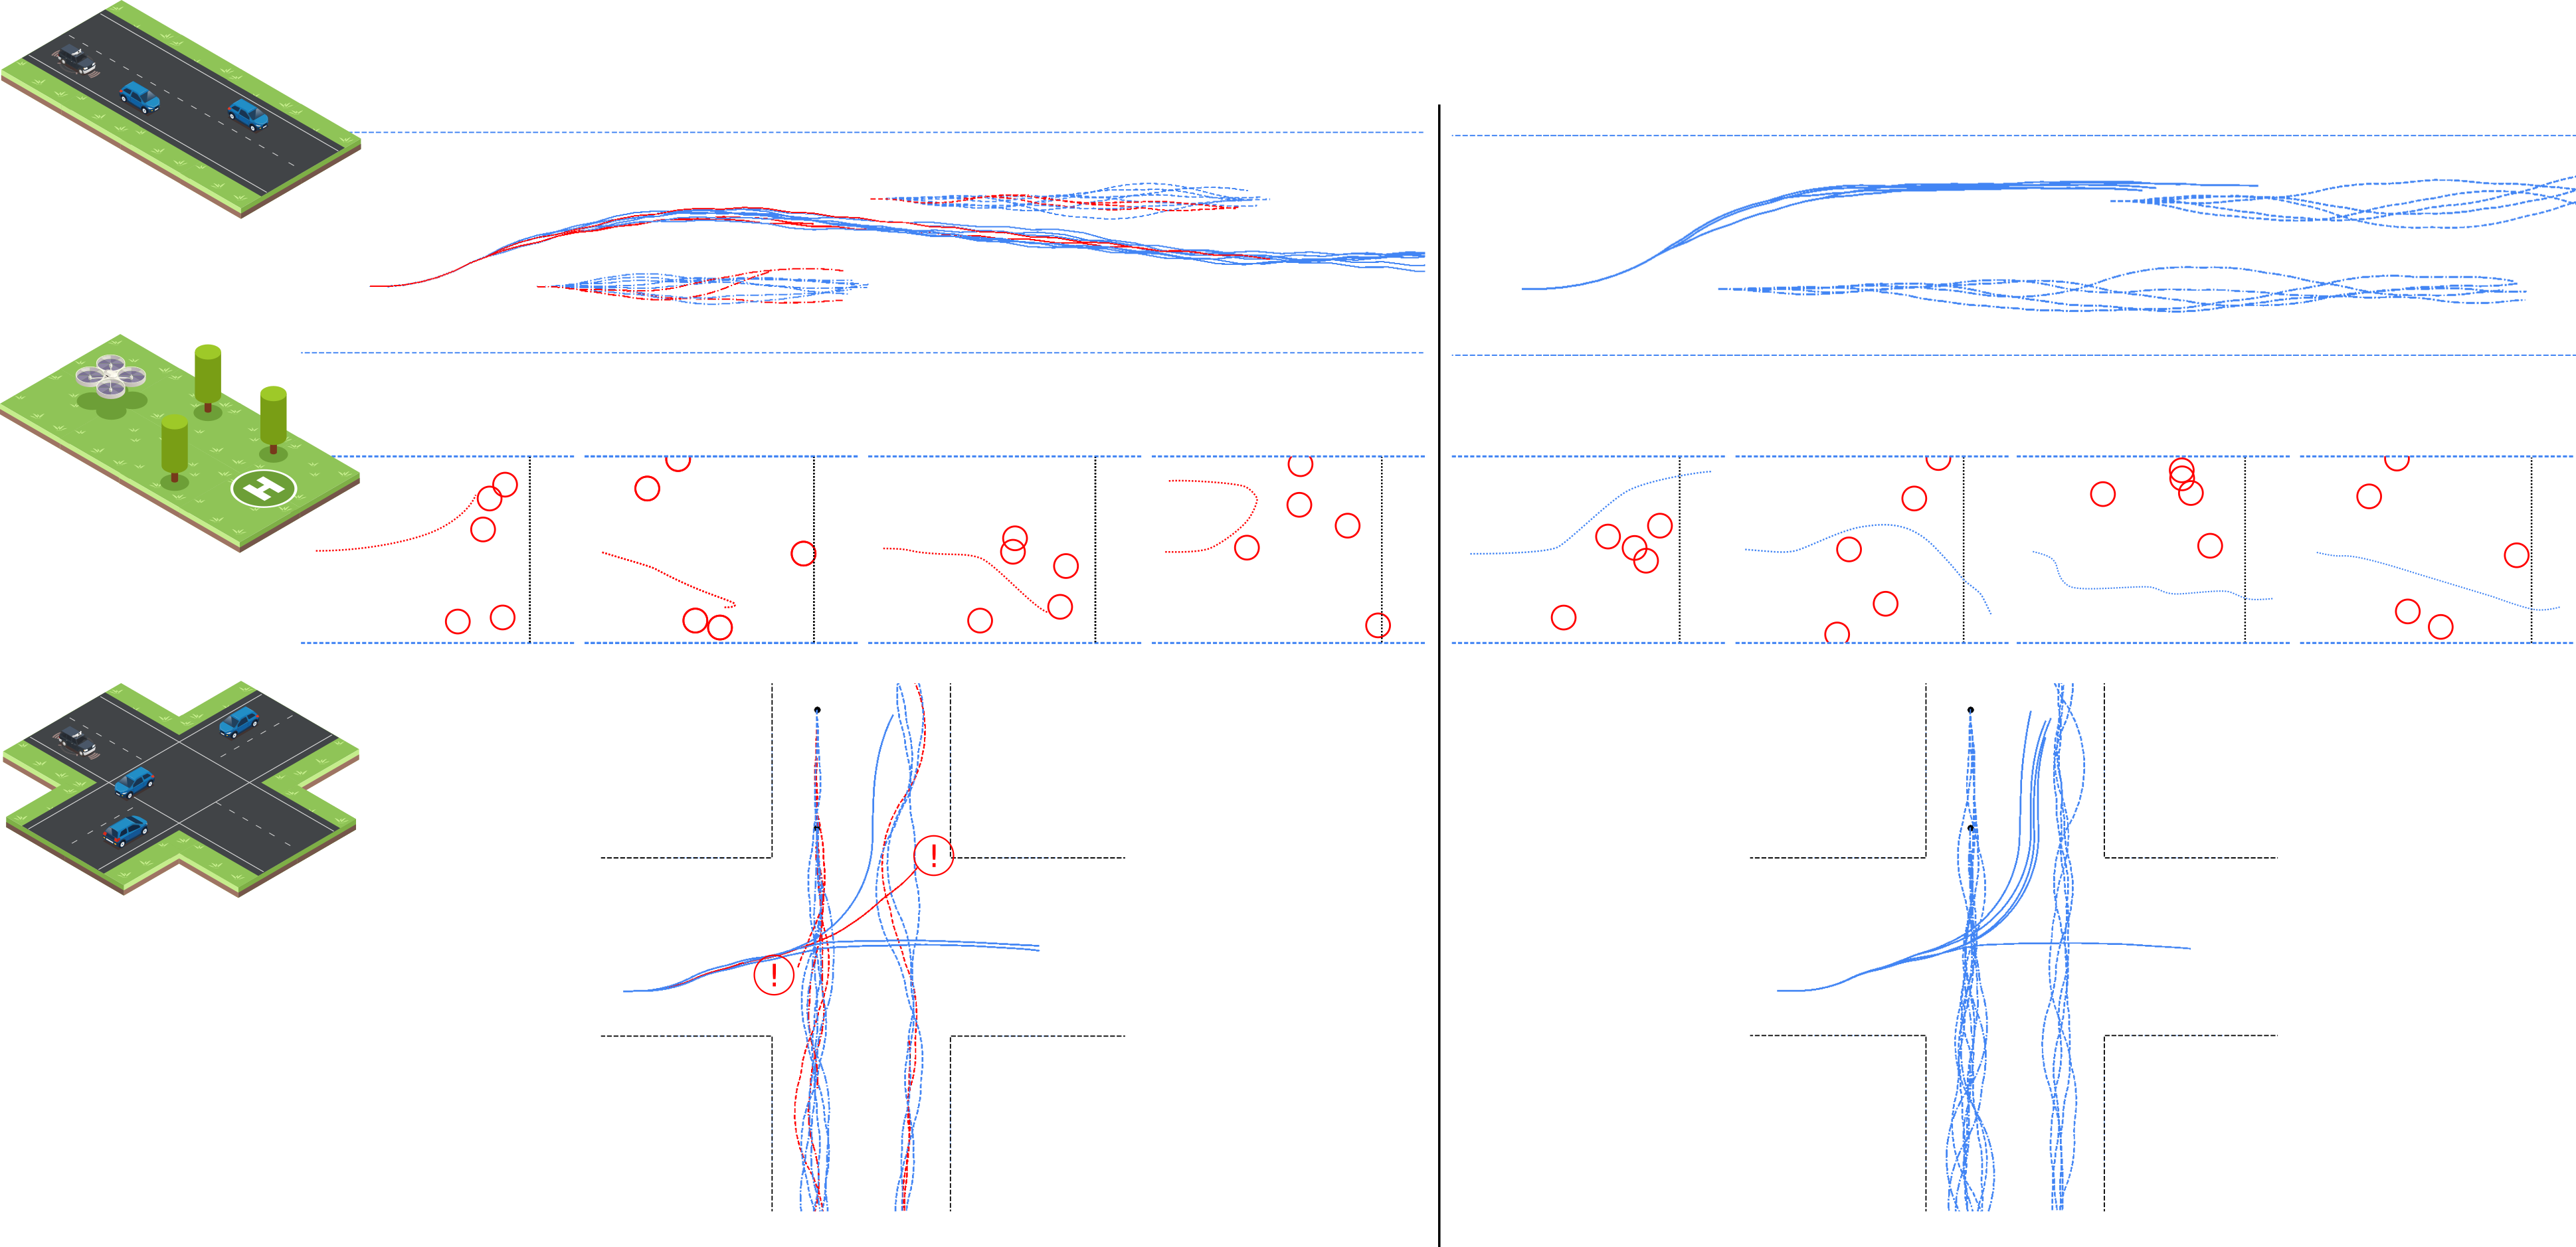
\includegraphics[width=\linewidth]{images/corl/repairs.png}
    \caption{Examples of failure cases (left) and repaired policies (right) generated using our method. Failed trajectories are shown in red.}\label{ch:corl:fig:repairs}
\end{figure}

\begin{table}
    \caption{Time required for simulating a rollout with and without autodiff (AD) for each task (in seconds). Average and standard deviation (subscript) reported across 100 trials on AMD Ryzen Threadripper 3990X 64-Core Processor (non-vision tasks) and an NVIDIA RTX A4000 (vision-in-the-loop tasks).}
    \label{ch:corl:tab:runtime}
    \centering
    \scriptsize
    \begin{tabular}{rcccccc}
        \toprule
        \multicolumn{1}{l}{} & \multicolumn{6}{c}{Non-vision tasks}                                                                                                                       \\
        \cmidrule(r){2-7}
                             & Power (14)                             & Power (57)         & Formation (5)     & Formation (10)               & Search (3v5)        & Search (12v20)      \\
        \midrule
        w/o AD               & $0.00122_{0.00413}$                    & $0.0107_{0.00893}$ & $0.0326_{0.0173}$ & $0.628_{0.296}$              & $0.00147_{0.00461}$ & $0.00461_{0.00747}$ \\
        w/ AD                & $0.00165_{0.00488}$                    & $0.0136_{0.0111}$  & $0.0543_{0.0212}$ & $0.714_{0.306}$              & $0.00358_{0.00704}$ & $0.0107_{0.00851}$  \\
        \midrule
        \multicolumn{1}{l}{} & \multicolumn{6}{c}{Vision-in-the-loop}                                                                                                                     \\
        \cmidrule(r){2-7}
                             & AV (hw.)                               & AV (int.)          & Drone             & Grasp (all)                  &                     &                     \\
        \midrule
        w/o AD               & $0.70_{0.003}$                         & $2.22_{0.01}$      & $0.39_{0.002}$    & $0.0045_{5.1\times 10^{-5}}$ &                                           \\
        w/ AD                & $1.72_{0.003}$                         & $6.65_{0.14}$      & $1.77_{0.06}$     & $0.0049_{3.8\times 10^{-5}}$ &                                           \\
        \bottomrule
    \end{tabular}
\end{table}

\subsection{Discussion}

In our results on problems without vision in the loop (Fig.~\ref{ch:corl:fig:nonvision_results}), we see several high-level trends. First, we see that gradient-based techniques (\gdr, \gda, and $R_1$) achieve lower failure rates, mean cost, and 99\textsuperscript{th} percentile costs relative to gradient-free methods (\ltc{} and $R_0$) on the test set, likely because gradient information helps the former methods explore the high-dimensional search space (as seen in the faster convergence of gradient-based methods in Fig.~\ref{ch:corl:fig:convergence:nonvision}). Moreover, we find that our methods ($R_0$ and $R_1$) outperform other methods within each of their respective categories; i.e. $R_0$ yields repaired solutions with lower costs and failure rates than \ltc, and $R_1$ likewise outperforms \gdr{} and \gda{}.

We see a slightly different pattern in our results for problems with vision in the loop. On these problems, we find that existing gradient-based methods like \gda{} do not achieve lower failure rates than gradient-free methods like \ltc{}, possibly due to poor gradient quality from the differentiable renderer (where occlusions can lead to large variance in the automatically-derived gradients). In contrast, both variants of our method achieve low failure rates for repaired policies in the vision-in-the-loop tasks, and $R_1$ in particular is able to achieve better performance on some tasks because the Metropolis-Hastings adjustment on line~\ref{ch:corl:alg:mala:mh} of Algorithm~\ref{ch:corl:alg:mala} allows it to reject large steps caused by poorly conditioned gradients.

\section{Case studies}\label{ch:corl:case_studies}

In this next section, we present three case studies to illustrate the practical use of our method. We first demonstrate how RADIUM can be used to solve a challenging optimization problem arising in the control of electrical power systems. We then provide two case studies showing how RADIUM can be applied to robotics problems and transferred to hardware, including one case study demonstrating sim2real transfer of vision-in-the-loop robot control policies.

\subsection{Robust generation dispatch for secure power networks}

For our first case study, we consider the problem of controlling an electric power grid subject to failures in transmission lines. Two simple networks (the IEEE 14- and 57-node test system) are shown in Fig.~\ref{ch:corl:fig:networks}. The goal in this problem is to find control inputs (power injection and voltage at each generator, and power demand at each load) that ensure that the voltage seen by each load is stable, even in the event of transmission outages (which we model using a bimodal distribution for the admittance of each line). The simulator models the AC power flow through this network, and the cost function penalizes excessively high or low voltages or any violation of rated generator capacities. More details on this motivating example is provided in the appendix.

Given a transmission network, the so-called \textit{security-constrained optimal power flow problem} (or SCOPF~\cite{capitanescuStateoftheartChallengesFuture2011}) is the problem of scheduling generator setpoints and power demand from loads to minimize the economic cost of generation and ensure that the network operates safely (satisfying voltage and maximum power constraints) in the event of transmission line outages. The design parameters $x = (P_g, |V|_g, P_l, Q_l)$ include the real power injection $P_g$ and AC voltage amplitude $|V|_g$ at each generator in the network and the real and reactive power draws at each load $P_l, Q_l$; all of these parameters are subject to minimum and maximum bounds that we model using a uniform prior distribution $p_{x, 0}$. The exogenous parameters are the state $y_i \in \R$ of each transmission line in the network; the admittance of each line is given by $\sigma(y_i) Y_{i, nom}$ where $\sigma$ is the sigmoid function and $Y_{i, nom}$ is the nominal admittance of the line. The prior distribution $p_{y, 0}$ is an independent Gaussian for each line with a mean chosen so that $\int_{-\infty}^0 p_{y_i, 0}(y_i) dy_i$ is equal to the likelihood of any individual line failing (e.g. as specified by the manufacturer; we use $0.05$ in our experiments). The simulator $S$ solves the nonlinear AC power flow equations~\cite{cainHistoryOptimalPower2012} to determine the state of the network, and the cost function combines the economic cost of generation $c_g$ (a quadratic function of $P_g, P_l, Q_l$) with the total violation of constraints on generator capacities, load requirements, and voltage amplitudes:
\begin{align}
    J = & c_g + v(P_g, P_{g, min}, P_{g, max}) + v(Q_g, Q_{g, min}, Q_{g, max}) \\
        & + v(P_l, P_{l, min}, P_{l, max}) + v(Q_l, Q_{l, min}, Q_{l, max})     \\
        & + v(|V|, |V|_{min}, |V|_{max}) \label{ch:corl:eq:scopf_cost}
\end{align}
where $v(x, x_{min}, x_{max}) = L\pn{[x - x_{max}]_+ + [x_{min} - x]_+}$, $L$ is a penalty coefficient ($L=100$ in our experiments), and $[\circ]_+ = \max(\circ, 0)$ is a hinge loss.

Efficient solutions to SCOPF are the subject of active research~\cite{capitanescuStateoftheartChallengesFuture2011,u.s.departmentofenergyGridOptimizationCompetition}. In addition to its potential economic and environmental impact~\cite{cainHistoryOptimalPower2012}, SCOPF is also a useful benchmark problem for 3 reasons: 1) it is highly non-convex, 2) it has a large space of possible failures, and 3) it can be applied to networks of different sizes to test an algorithm's scalability. In our case, the 14-bus network has 32 design parameters and 20 exogenous parameters, while the 57-bus network has 98 design parameters and 80 exogenous parameters.

\begin{figure}[tb]
    \centering
    \begin{subfigure}[t]{0.4\linewidth}
        \centering
        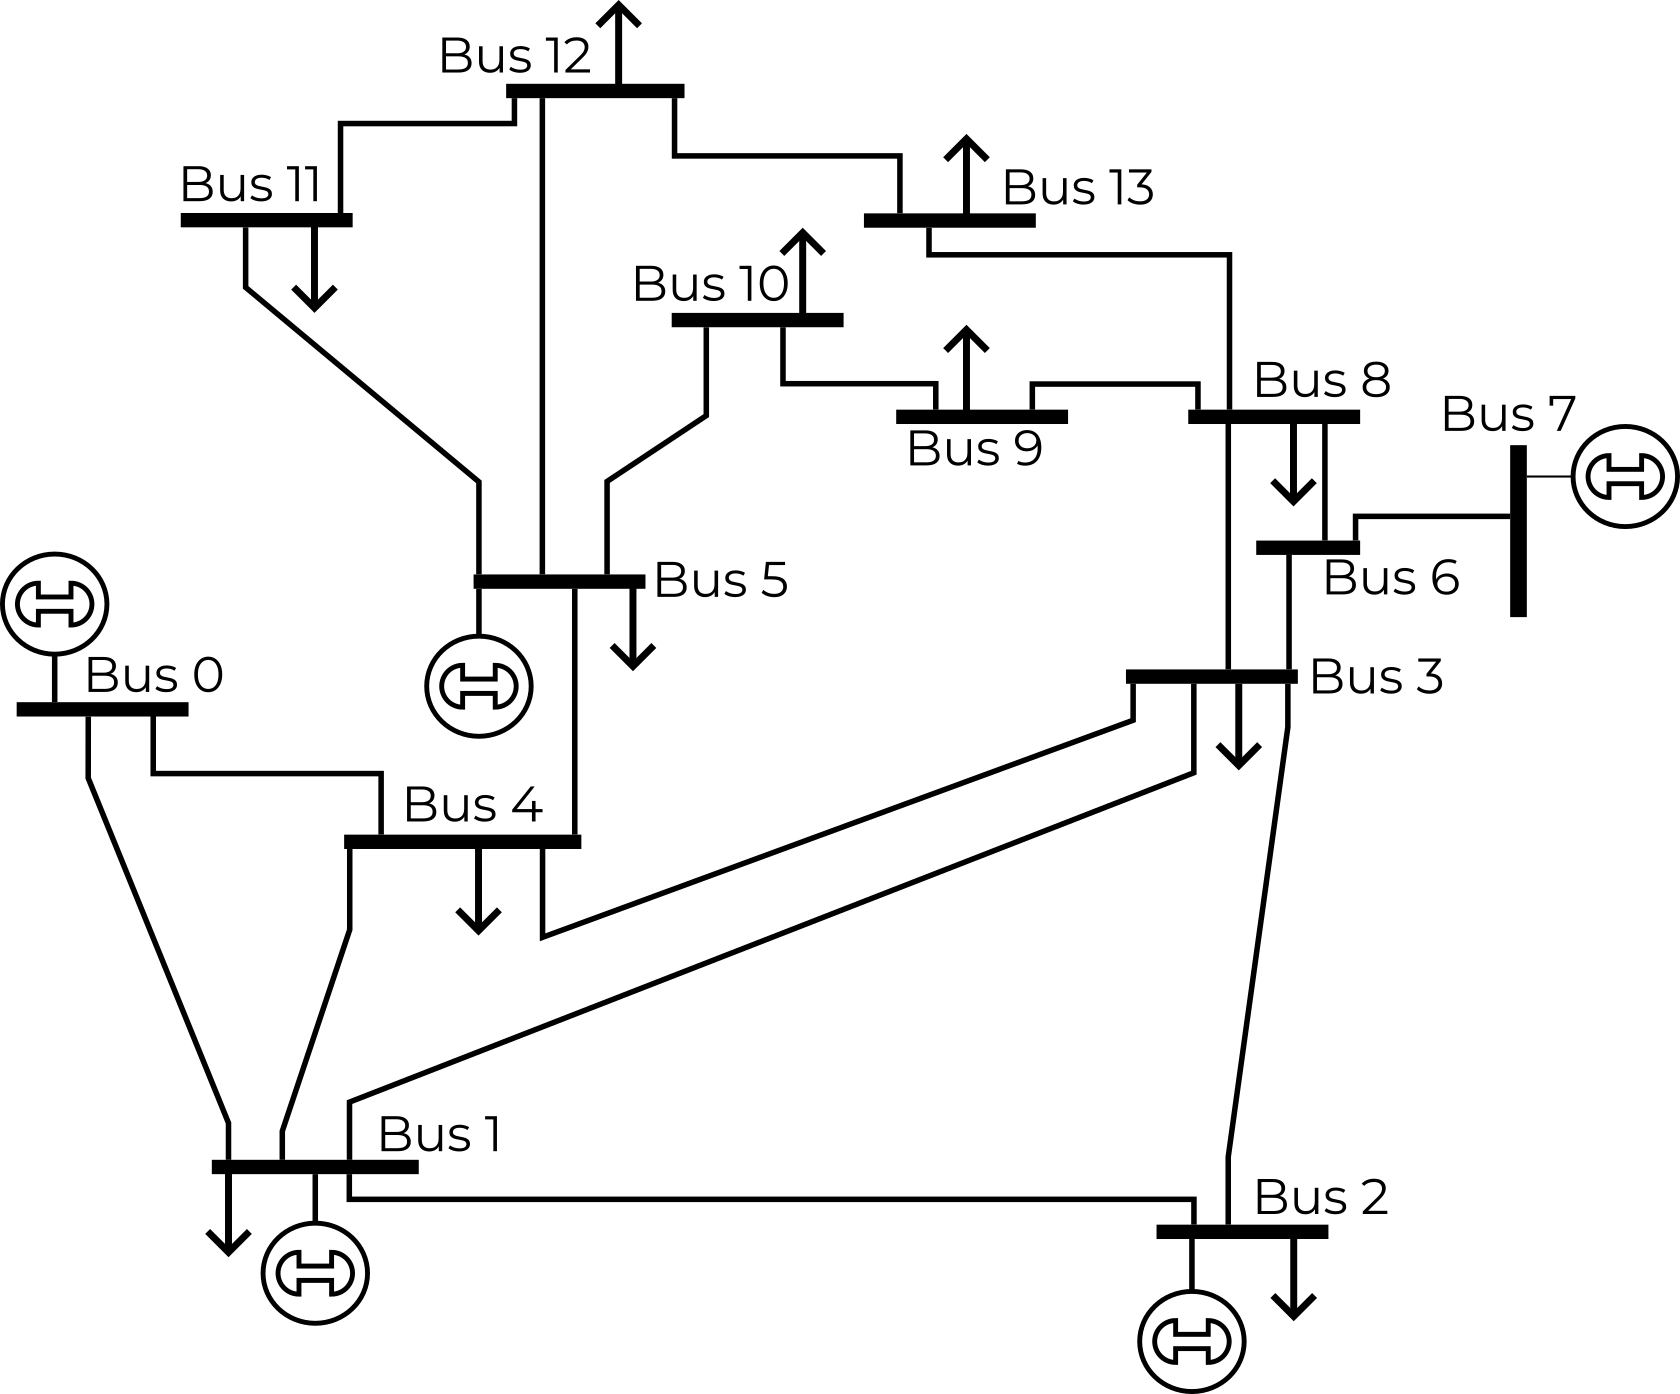
\includegraphics[width=\linewidth]{images/global_methods/base_14_bus.png}
    \end{subfigure}
    \begin{subfigure}[t]{0.4\linewidth}
        \centering
        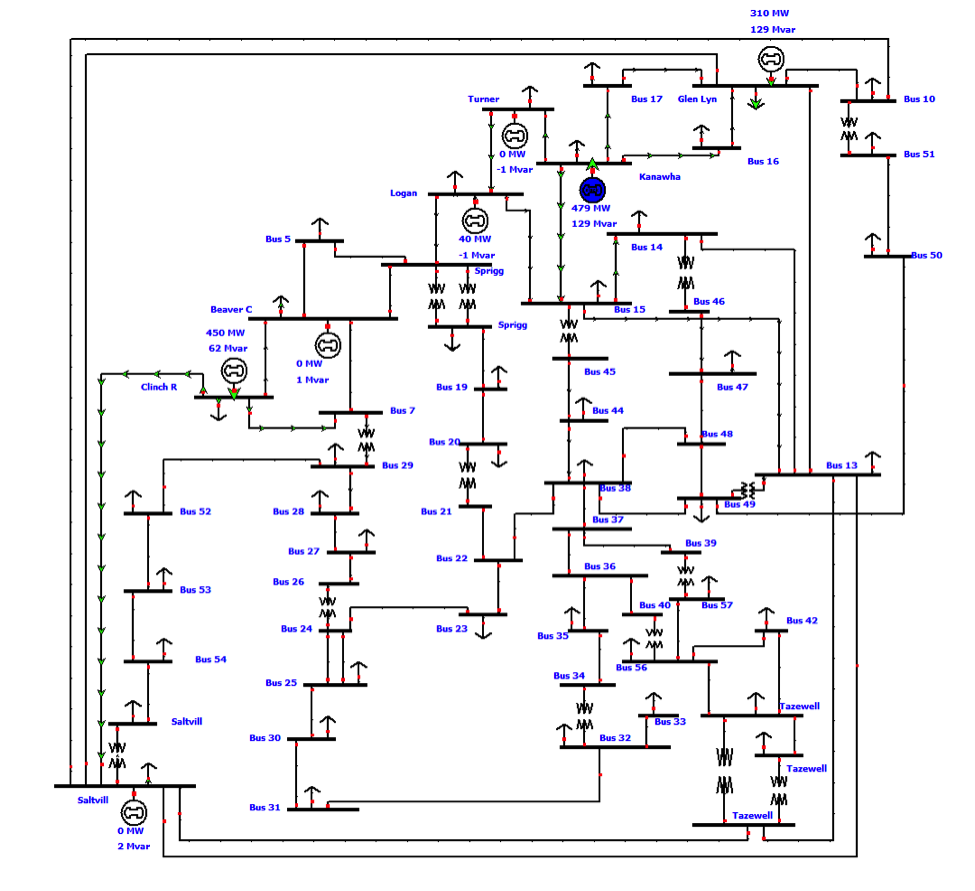
\includegraphics[width=\linewidth]{images/global_methods/IEEE57.png}
    \end{subfigure}%
    \caption{Example 14- and 57-bus electricity transmission networks~\cite{illinoiscenterforasmarterelectricgridIEEE57BusSystem}.}
    \label{ch:corl:fig:networks}
\end{figure}

A high-level comparison of RADIUM with existing methods on these SCOPF problems is shown in Figs.~\ref{ch:corl:fig:nonvision_results} and~\ref{ch:corl:fig:convergence:nonvision}; in this section, we provide a more detailed comparison between RADIUM and optimization-based methods that are the state-of-the-art for this SCOPF problem~\cite{dontiAdversariallyRobustLearning2021} (the comparison with \ltc{} is not shown in this section, since it is not able to solve the SCOPF problem).

\paragraph{Solution quality} To compare the quality of these methods' solutions, we use each method to optimize $10$ candidate designs and predict $10$ failure modes using Algorithm~\ref{ch:corl:alg:adv_diffusion}. We then select the design that achieves the highest likelihood according to Eq.~\eqref{ch:corl:eq:repair_logprob_tempered}, then use one additional round to sample new failure modes that attack the chosen design. The maximum cost across these final predicted failure modes provides a measure of each algorithm's confidence in its solution. We then compare the performance on these predicted failure modes to the maximum cost observed on a test set of $10^6$ exogenous parameters sampled randomly from the prior $p_{y, 0}$. Fig.~\ref{ch:corl:fig:scopf_comparison:14_bus} shows the predicted and observed costs for each method on the IEEE 14-bus test case. The prediction-and-mitigation process takes \SI{30.5}{s} for \gdr{}, \SI{61.5}{s} for \gda{}, \SI{111.5}{s} for $R_0$, and \SI{141.7}{s} for $R_1$ (including the cost of JAX just-in-time compilation).

\begin{figure}[tb]
    \centering
    \begin{subfigure}[t]{0.45\linewidth}
        \centering
        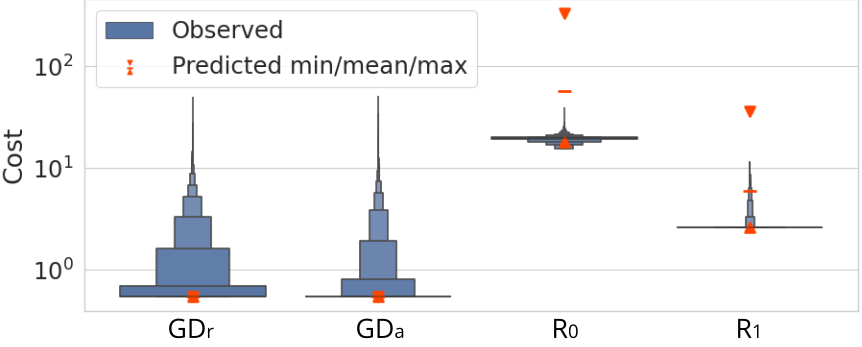
\includegraphics[width=\linewidth]{images/global_methods/14_bus_comparison.png}
        \caption{14-bus network}\label{ch:corl:fig:scopf_comparison:14_bus}
    \end{subfigure}
    \begin{subfigure}[t]{0.45\linewidth}
        \centering
        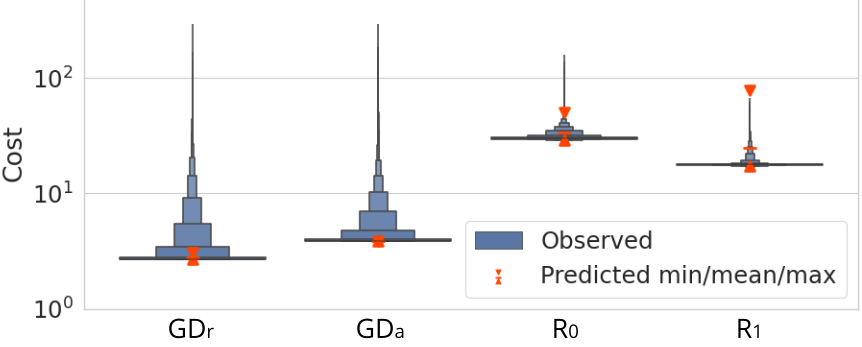
\includegraphics[width=\linewidth]{images/global_methods/57_bus_comparison.png}
        \caption{57-bus network}\label{ch:corl:fig:scopf_comparison:57_bus}
    \end{subfigure}
    \caption{Comparison of our method with baselines for failure prediction and mitigation on power transmission networks. Red markers show the maximum, mean, and minimum-cost failure modes predicted by each method after optimizing the design, while the box plot shows the distribution of costs on a test set of $10^6$ random failures.}
    \label{ch:corl:fig:scopf_comparison}
\end{figure}

We can assess these methods in two ways: by the quality of the optimized design and by the quality of the predicted failure cases. The two optimization-based methods, \gda{} and \gdr{}, find solutions with the lowest best-case cost, but their solutions are not robust. Not only do these methods find solutions that are susceptible to a heavy tail of failures, but they are overconfident and fail to predict those failures (instead predicting that all 10 candidate failures will be successfully mitigated). In contrast, $R_0$ is not overconfident (it successfully predicts failure modes that match the range of the empirical failure distribution), but it finds a solution that is 10 times costlier than those found by $R_1$. Only $R_1$ is able to find a robust, low-cost solution without being overconfident.

Once we have a robust design optimized using our method, we can examine the predicted failure modes to understand the remaining ways in which our design might fail. Of the ten failure modes predicted by $R_1$, four include attacks on the transmission line connecting the generator at bus 7 to the rest of the network (this was the most commonly attacked line). Interestingly, of these four attacks, only one (shown in Fig.~\ref{ch:corl:fig:predicted_failure_modes}) is able to cause a violation of the voltage stability constraints. It is only by fully disconnecting the generator at bus 7 (dotted red line) and partially impairing the line between buses 1 and 4 (solid red; $15\%$ impairment) that we see the voltage drop at several buses (shown in orange). This information about potential failure modes can be very useful to system designers; in this example, the designer may choose to focus monitoring and infrastructure hardening efforts on the two affected lines.

\begin{figure}[tb]
    \centering
    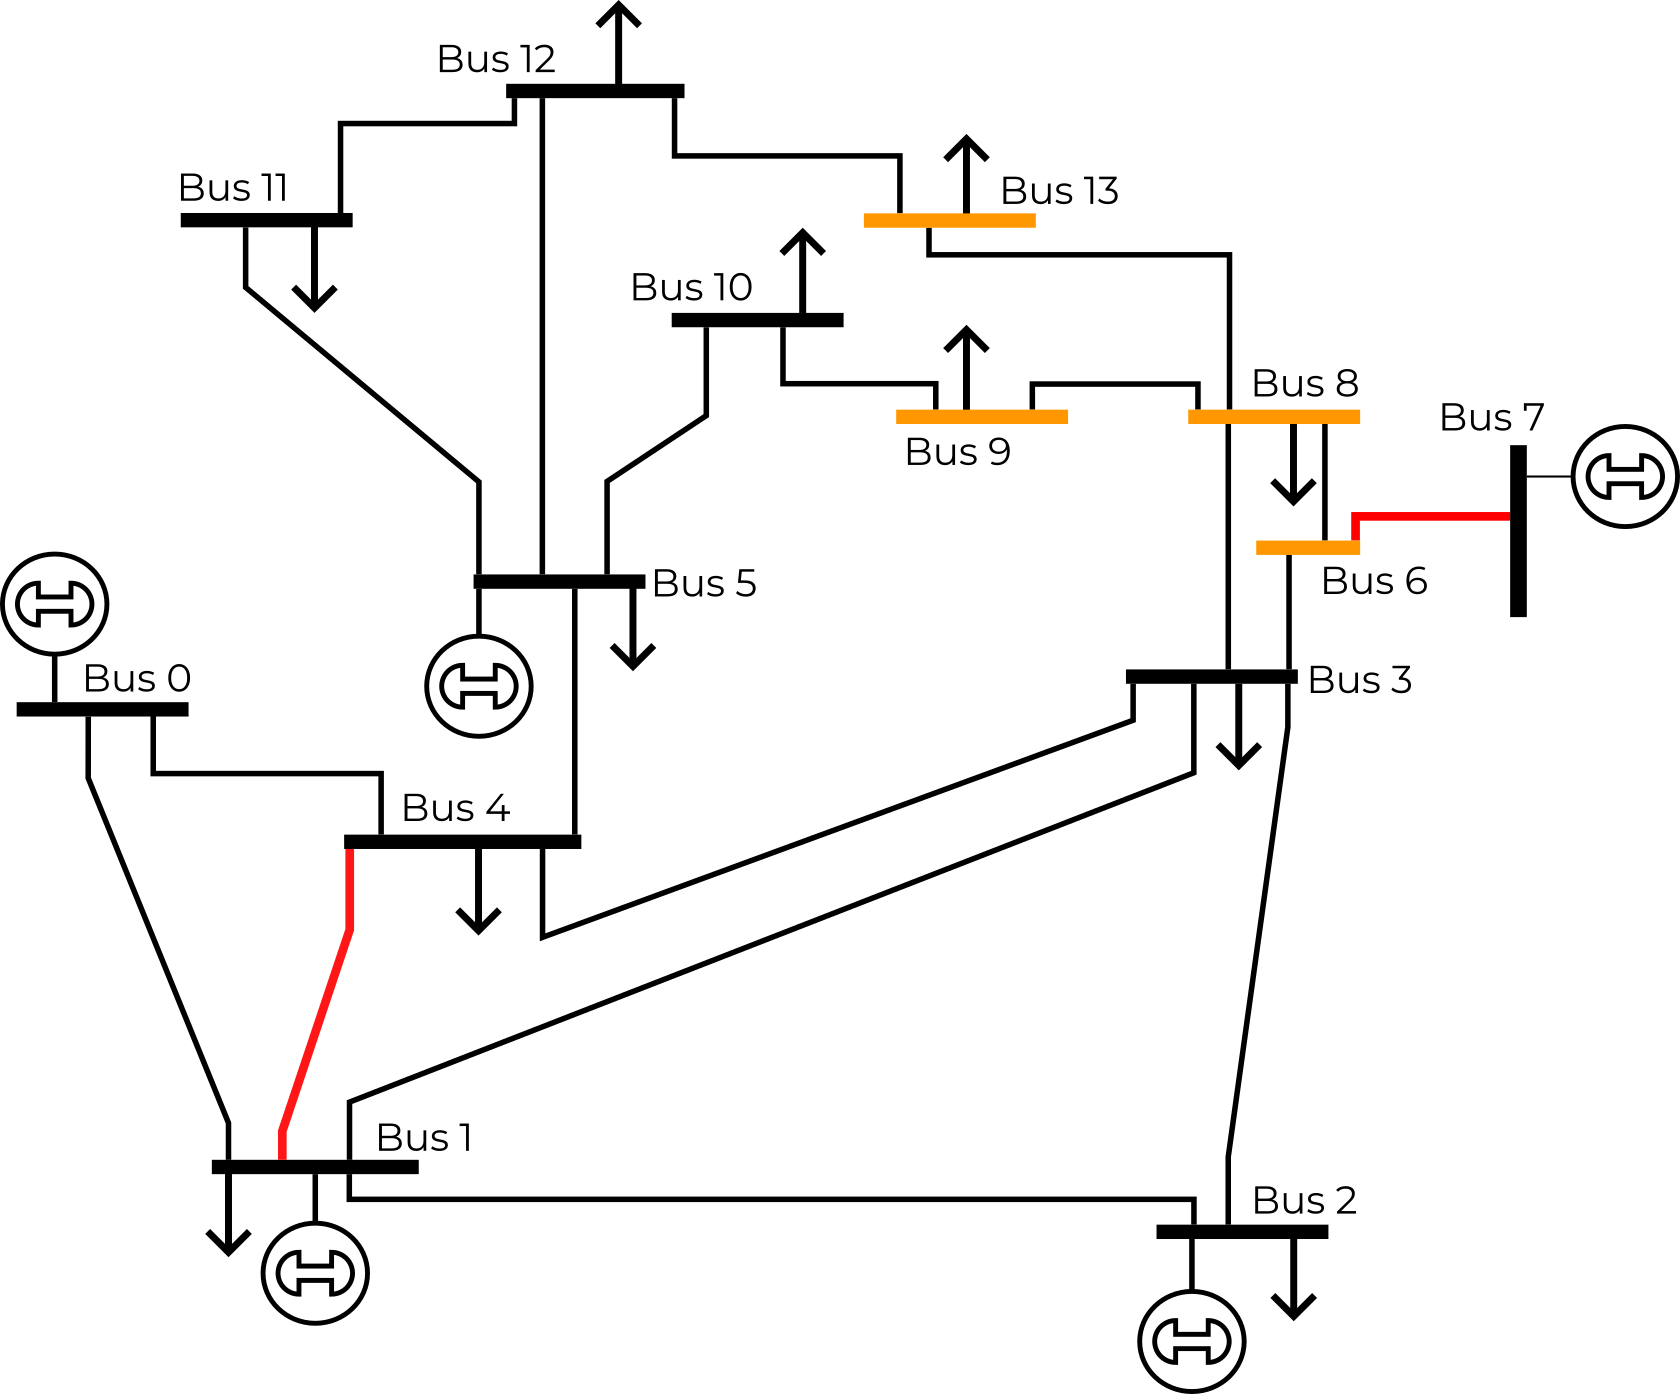
\includegraphics[width=0.4\linewidth]{images/global_methods/predicted_failure_modes.png}
    \caption{The only predicted failure modes (of 10 candidates) that causes violation of voltage constraints on the 14-bus transmission network, using the optimized design found using $R_1$. Fully disconnecting the generator at bus 7 (dotted red line) is not enough; other predicted failures include this outage but do not cause a constraint violation. It is only by additionally impairing the line between buses 1 and 4 that the voltage constraint is violated at the buses shown in orange.}
    \label{ch:corl:fig:predicted_failure_modes}
\end{figure}

To understand the scalability of our approach, we repeat this experiment on a larger 57-bus network with 80 transmission lines. All hyperparameters were the same except for the step size for exogenous parameters, which was reduced to $10^{-3}$. The results are shown in the bottom panel of Fig.~\ref{ch:corl:fig:scopf_comparison:14_bus}; we see that $R_1$ continues to not only find a robust solutions (with a relatively light tail of failures) but also accurately predicts the range of possible failure modes ($R_0$ does not explore the full failure space in this case). Running \gdr{} on this example takes \SI{406.2}{s}, \gda{} takes \SI{803.4}{s}, $R_0$ takes \SI{1002.3}{s}, and $R_1$ takes \SI{1438.5}{s}.

\paragraph{Convergence rate} From comparing solution quality, there is a clear separation between the sampling- and optimization-based methods, with sampling able to find more robust designs and more accurately cover the range of possible failures (although gradient-based sampling finds higher-quality solutions than gradient-free sampling in both cases). A natural next question is how quickly these methods converge to a solution.

To measure the relative convergence rate of \gdr{}, \gda{}, $R_0$, and $R_1$, we measure the 99\textsuperscript{th} percentile cost $J$ of the candidate design $[x]_i$ with the highest log likelihood~\eqref{ch:corl:eq:repair_logprob_tempered} on a test set of 1000 exogenous parameters sampled randomly from the prior. The convergence of this test-set performance as a function of the number of sampling rounds is shown in Fig.~\ref{ch:corl:fig:power_training_curves} for both the 14- and 57-bus networks.

\begin{figure}[tb]
    \centering
    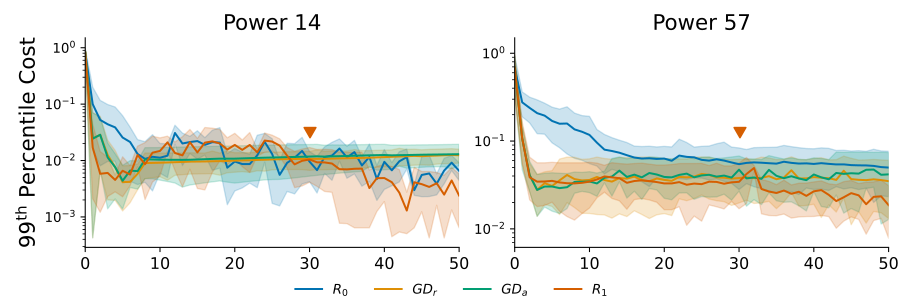
\includegraphics[width=\linewidth]{images/corl/power_convergence.png}
    \caption{Comparison of convergence rates of different methods on 14- (left) and 57-bus (right) power networks, showing the 99\textsuperscript{th} percentile cost of the best design after each round. The {\color{orange} $\blacktriangledown$} symbol indicates the start of quenching for $R_1$.}
    \label{ch:corl:fig:power_training_curves}
\end{figure}

There are two important conclusions to be drawn from comparing the convergence rates in Fig.~\ref{ch:corl:fig:power_training_curves}. The first is that the gradient-based methods, \gdr{}, \gda{}, and $R_1$, converge faster than gradient-free $R_0$. Although the SCOPF problem (as well as ACOPF, the non-adversarial version) are non-convex optimization problems, there are known convex relaxations~\cite{huangReviewConvexificationMethods2019}, and gradient descent-based methods have been shown to work well for finding local optima~\cite{dontiAdversariallyRobustLearning2021,dontiDC3LearningMethod2021}, so the good performance of gradient-based methods is not surprising.

The second important conclusion from Fig.~\ref{ch:corl:fig:power_training_curves} is the importance of quenching $R_1$ on this problem (i.e. disabling the stochastic part of the sampling algorithm and taking a few gradient descent steps during the final rounds). Prior to quenching, $R_1$ converges to a solution with similar 99\textsuperscript{th} percentile cost as \gdr{} and \gda{}, but after quenching (in the last 20 rounds), $R_1$ is able to find a solution with a much lower cost. This is likely because of the constraints on $P$, $Q$, and $|V|$ in the SCOPF problem; sampling based methods may struggle to exactly satisfy constraints like these, as $MALA$ and $RMH$ are constantly injecting noise into the solution, and so running a few steps of gradient descent on $\theta$ towards the end of the repair process likely helps drive constraint violations to zero by converging to the local minima nearest to the solutions explored by the sampling process. The fact that $R_1$ converges to a lower-cost solution than \gdr{} or \gda{}, despite running the same gradient-based optimization process during the quenching phase, suggests that the improved exploration of designs and failures due to sampling provides an advantage over pure optimization-based methods on this problem.

\subsection{Multi-agent control and path planning}

We return to the search problem used as a baseline in Section~\ref{ch:corl:experiments}, where a team of seeker robots must cover a region to detect a set of hiders. The simulation environment includes $n_{seek}$ seeker robots and $n_{hide}$ hider robots. Each robot is modeled using single-integrator dynamics and tracks a pre-planned trajectory using a proportional controller with saturation at a maximum speed chosen to match that of the Robotarium platform~\cite{wilsonRobotariumGloballyImpactful2020}. The trajectory $\vec{x}_i(t)$ for each robot is represented as a Bezier curve with 5 control points $\vec{x}_{i, j}$,
\begin{align*}
    \vec{x}_i(t) = \sum_{j=0}^4 \binom{4}{j}(1-t)^{4-j}t^j \vec{x}_{i, j}
\end{align*}

The design parameters are the 2D position of the control points for the trajectories of the seeker robots, while the exogenous parameters are the control points for the hider robots. The prior distribution for each set of parameters is uniform over the width and height of the Robotarium arena ($\SI{3.2}{m}\times\SI{2}{m}$).

We simulate the behavior of the robots tracking these trajectories for \SI{100}{s} with a discrete time step of \SI{0.1}{s} (including the effects of velocity saturation that are observed on the physical platform), and the cost function is
\begin{align*}
    J = \sum_{i=1}^{n_{hide}}\pn{\mathop{\widetilde{\min}}_{t = t_0, \ldots, t_{n}} \pn{\mathop{\widetilde{\min}}_{j=1, \ldots, n_{seek}}\norm{\vec{p}_{hide, i}(t) - \vec{p}_{seek, j}(t)} - r}}
\end{align*}
%
where $r$ is the sensing range of the seekers (\SI{0.5}{m} for the $n_{seek} = 2$ case and \SI{0.25}{m} for the $n_{seek}=3$ case); $\widetilde{\min}(\cdot) = -\frac{1}{b}\text{logsumexp}(-b\ \cdot)$ is a smooth relaxation of the element-wise minimum function where $b$ controls the degree of smoothing ($b=100$ in our experiments); $t_0, \ldots, t_{n}$ are the discrete time steps of the simulation; and $\vec{p}_{hide, i}(t)$ and $\vec{p}_{seek, j}(t)$ are the $(x, y)$ position of the $i$-th hider and $j$-th seeker robot at time $t$, respectively. In plain language, this cost is equal to the sum of the minimum distance observed between each hider and the closest seeker over the course of the simulation, adjusted for each seeker's search radius.

We deploy the optimized hider and seeker trajectories in hardware using the Robotarium multi-robot platform~\cite{wilsonRobotariumGloballyImpactful2020} (we use 3 seekers and 5 hiders, since we had difficulty testing with more agents in the limited space). We first hold the search pattern (design parameters) constant and optimize evasion patterns against this fixed search pattern, yielding the results shown on the left in Fig.~\ref{fig:hw_experimental_results} where the hiders easily evade the seekers. We then optimize the search patterns using our approach (with $K=100$ rounds and $M=10$ substeps per round, taking \SI{41}{s}), yielding the results on the left where the hiders are not able to evade the seekers. Trajectories for the hiders and seekers were planned offline and then tracked online using linear trajectory-tracking controllers.

\begin{figure}[tb]
    \centering
    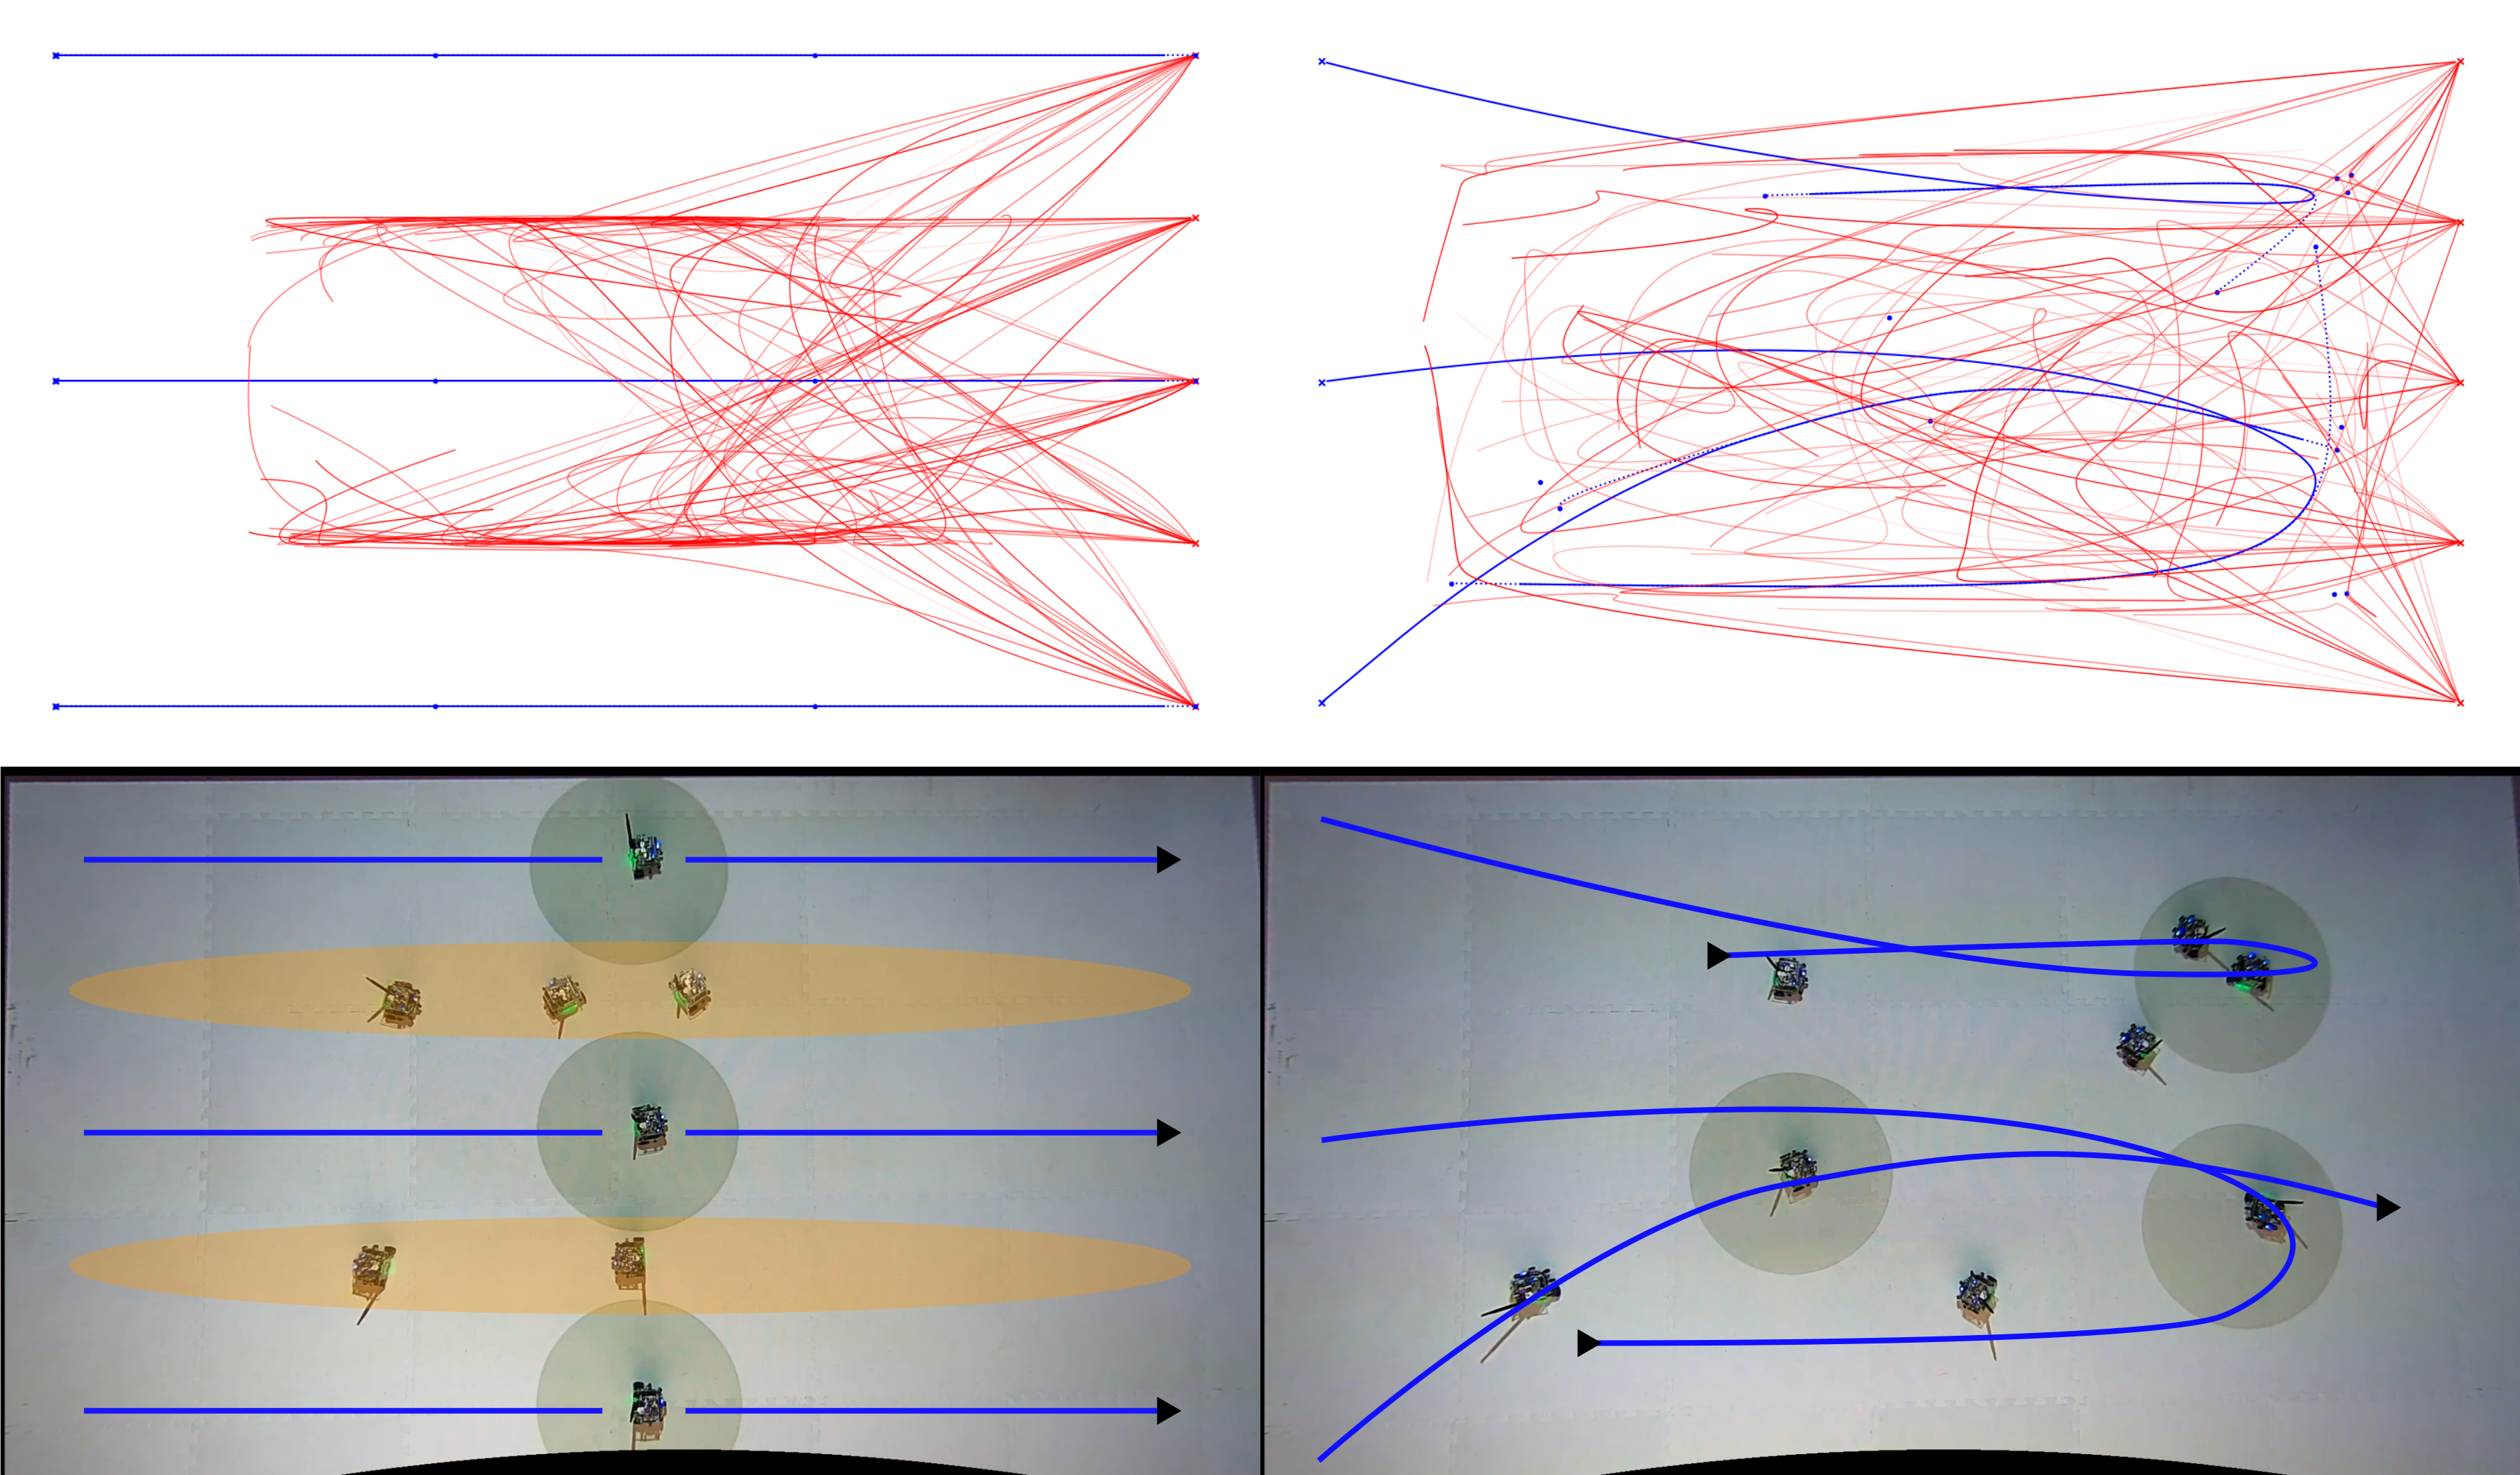
\includegraphics[width=\linewidth]{images/corl/hw_results.png}
    \caption{(Left) HW results for search-evasion with 5 hiders and 3 seekers, showing an initial search pattern (seeker trajectories; blue) and predicted failure modes (hider trajectories; red). (Right) HW results for an optimized search pattern leaves fewer hiding places. The top row shows the predicted failure modes (i.e. hider trajectories), while the bottom row shows a snapshot from hardware executions of these trajectories.}
    \label{fig:hw_experimental_results}
\end{figure}

Although the gap between simulation and reality is not particularly large in this case, there are effects present in the hardware system that we did not model in our simulator (e.g. the collision-avoidance safety filter used by the Robotarium). Despite this small gap, this case study serves as a useful proof-of-concept for transferring optimized designs from simulation to hardware.

In the next case study, we will demonstrate the transfer of failure modes and repaired designs in a much more challenging environment with vision in the loop.

\subsection{Vision-in-the-loop control of a 1/10-scale race car}

In our simulation studies in Section~\ref{ch:corl:experiments}, we introduced a highway driving task where an autonomous vehicle must overtake two slower cars using visual feedback to avoid collision with other agents. In this case study, we return to this example, developing a hardware test environment where the autonomous agent controls a 1/10\textsuperscript{th}-scale race car and the two non-ego agents are represented by TurtleBots.

We pre-train a policy for the highway task that has three components: a tracking controller that follows a pre-planned trajectory, a model-based collision avoidance controller that attempts to avoid rear-ending cars in front of the ego vehicle (using the depth camera to measure the distance to the next car), and a neural network controller that accelerates and steers based on the depth image received from a forward facing camera. The parameters of the neural network and the pre-planned trajectory are optimized via vanilla gradient descent during pre-training. The cost function is the negative minimum reward observed during each rollout:
\begin{align}
    J   & = -\widetilde{\min}_t\pn{r_t}            \\
    r_t & = 0.1 (x_t - x_{t-1}) - 5 \sigma(-5 d_t)
\end{align}
where $\widetilde{\min}_t$ is a soft minimum (as defined in Chapter~\ref{ch:iros}) over time, with sharpness parameter $10$. $r_t$ is the reward at each timestep, defined as the weighted sum of the distance traveled along the highway and a term that penalizes collisions. $\sigma$ is the sigmoid function and $d_t$ is the minimum distance between the ego vehicle and the nearest obstacle at time $t$.

We then use $R_1$ to predict failure modes for this pre-trained, vision-in-the-loop policy in simulation, then transfer both the pre-trained policy and predicted failure modes to hardware. As shown in Fig.~\ref{ch:corl:fig:hw:car:fail}, the failure modes predicted in simulation correspond to real failures on hardware. We then repair the policy using $R_1$, which results in an updated policy and new predicted worst-case failure mode, shown in Fig.~\ref{ch:corl:fig:hw:car:repair}. Since $R_1$ predicts different failure modes for the nominal and repaired policies, Table~\ref{ch:corl:tab:hw:metrics} compares the failure rates of both policies on 20 independent samples of $\phi$ from the prior distribution, showing that the repaired policy is 5x safer than the original policy.

These results demonstrate that both the predicted failure modes and the repaired policy can successfully transfer from simulation to hardware, despite the gap between the simulated dynamics and rendering system and reality. A benefit of the sampling-based approach proposed in $R_0$ and $R_1$ is that the noise added during the sampling step helps us avoid converging to narrow local minima, avoiding failures that occur only due to quirks in the simulation environment.

\begin{figure}[tb]
    \centering
    \subfloat[Nominal policy]{
        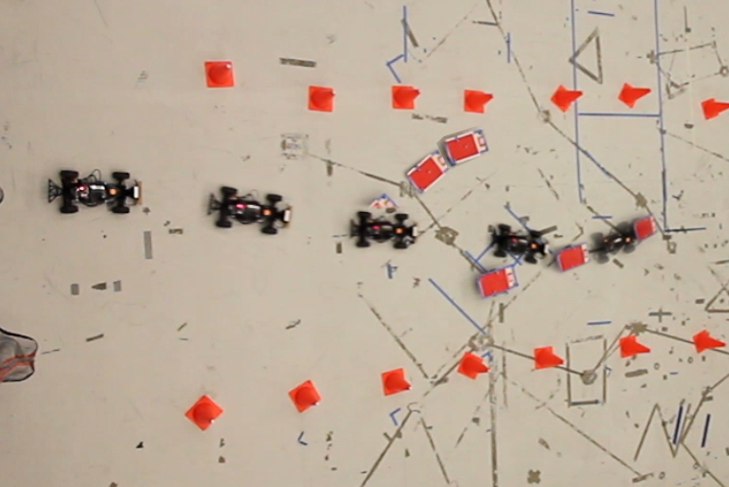
\includegraphics[height=6cm]{images/corl/f1tenth/nominal_crash/composite_cropped.png}
        \label{ch:corl:fig:hw:car:fail}
    }
    \subfloat[Repaired policy]{
        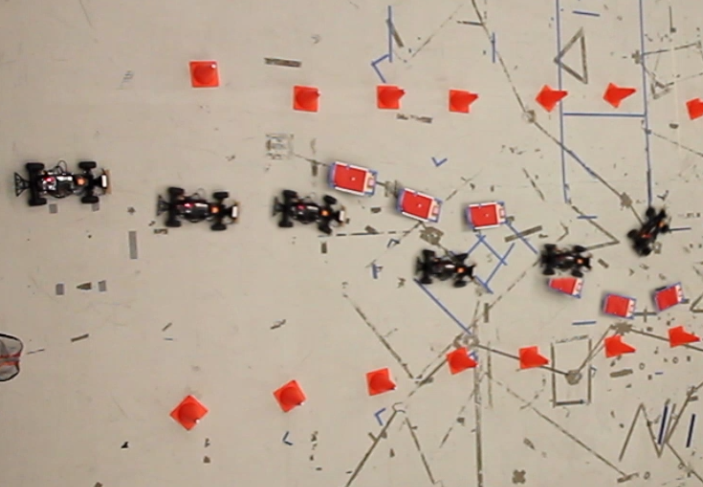
\includegraphics[height=6cm]{images/corl/f1tenth/repaired_nocrash/composite_crop.png}
        \label{ch:corl:fig:hw:car:repair}
    }
    \caption{Composite images from hardware experiments with vision-in-the-loop controllers. (Left) the nominal policy and the worst adversarial example found using our method, where a crash occurs. (Right) the repaired policy and new worst adversarial example (both found using our method); the repaired policy avoids crashing in this case.}
    \label{ch:corl:fig:hw:car}
\end{figure}

\begin{table}[htb]
    \caption{
        Failure rate on 1000 simulated and 20 hardware trials of nominal and repaired policies with exogenous parameters sampled i.i.d. from the prior $p_{\phi, 0}$.
    }
    \label{ch:corl:tab:hw:metrics}
    \begin{center}
        \begin{tabular}{lcc}
            \toprule
            Policy   & Failure rate (simulation) & Failure rate (hardware) \\
            \midrule
            Nominal  & 4.4 \%                    & 25\%                    \\
            Repaired & 0.6 \%                    & 5\%                     \\
            \bottomrule
        \end{tabular}
    \end{center}
\end{table}

\section{Summary}

In this chapter, we close several key gaps in the prior work on adversarial design optimization. In particular, we reframe the adversarial optimization problem studied in Chapter~\ref{ch:iros} as a inference problem solved by sampling from specially constructed pseudo-posterior distributions. This reformulation brings three key advantages. First, it allows us to use gradient-based sampling algorithms that are robust to high-variance or poorly conditioned gradients that would otherwise cause a gradient-based optimization algorithm to diverge. Second, our stochastic sampling-based methods is able to avoid local minima that cause gradient-based optimizers to get stuck. Finally, since our method focused on sampling a range of high-severity failures, rather than finding a single most-severe failure, we are able to find a much more diverse set of counterexamples than prior optimization-based methods. Ultimately, these diverse counterexamples allow us to optimize against a more challenging curriculum of failure modes, leading to more robust designs.

We apply our approach to a range of robotics and cyberphysical control problems, demonstrating how the use of gradients from differentiable simulation and rendering can help accelerate convergence. However, we acknowledge that a differentiable simulation environment is not always available, and that substantial engineering effort can be required to develop such a simulator. Because of this difficulty, and because simulators of certain phenomena (e.g., contact~\cite{huDiffTaichiDifferentiableProgramming2019} and rendering with occlusion~\cite{zhaoPhysicsbasedDifferentiableRendering2020}) can yield inaccurate gradients if care is not taken, we build graceful degradation into our approach, providing a gradient-free version of our algorithm that can be used when gradients are not available. When gradient quality is poor, we find empirically that the acceptance rate of $R_1$ tends to zero, providing feedback to the user to either improve their differentiable simulator or switch to $R_0$ (which we find outperforms gradient-free baselines on the benchmark problems studied in this chapter).

Although the RADIUM framework developed in this chapter closes a number of important technical gaps from previous chapters, there are several limitations that remain to be addressed. First, these methods rely on a manually-specified cost function to define failures. For some complex systems, it may be difficult to specify an appropriate cost function \textit{a priori}, and doing so may lead our method to focus only on those failures defined by the cost function, preventing the discovery of other undesirable behaviors. Second, RADIUM relies entirely on simulation for discovering failures and repairing designs; although we can transfer RADIUM's designs and predicted failures from simulation to hardware, there is no immediately obvious way to feed the results of hardware experiments back into RADIUM. In the next chapter, we introduce a method for data-driven failure analysis that allows us to close the loop between simulation and real-world data, while avoiding the need for a hand-specified cost function.

% \chapter{Robust anomaly diagnosis with calibrating normalizing flows}\label{ch:icml}

The methods developed in previous chapters rely heavily on simulation to predict and repair failures in autonomous systems. Although simulation-driven testing is an important part of the development process for these systems, the ultimate goal is to deploy the system in the real world. Unfortunately, testing a system in the real world presents a number of challenges for the methods presented thus far in this thesis. Whereas simulation testing allows us to vary environmental parameters in order to preemptively predict failures, in reality we are often faced with the problem of analyzing a failure after the fact (often called a \textit{post-mortem} analysis). The goal of this analysis is to infer, based on data collected during a particular failure event, what went wrong; i.e. what changes in the environment were associated with the observed failure.

This analysis is challenging for a number of reasons. First, data collected from a system operating in the real world is often noisy and prone to outliers. Second, if we have been responsible in developing and deploying our system, failures should be relatively rare, meaning that while we may have a large amount of data from normal operation of the system, we typically have very little data from the failure itself. This data imbalance makes it difficult to apply many learning and inference methods directly to post-mortem analysis.

To formalize this problem, we can frame post-mortem analysis as a Bayesian inverse problem (IP), where we aim to infer the distribution of latent variables $z$ from noisy observations $x$ of a stochastic process $x \sim p(x | z; y)$, where $y$ are known context variables~\cite{stuartInverseProblemsBayesian2010,molinaroNeuralInverseOperators2023,liuOptimizationAmortizedInverse2023,asimInvertibleGenerativeModels2020}\footnote{In this chapter, we use $x$, $y$, and $z$ to denote the observation, context, and latent variables to align with standard inverse problem notation. In the context of the notation used in previous chapters, $x$ denotes the system's behavior, represented as a trace of states $s_1, \ldots, s_T$, while $y$ and $z$ denote known and unknown components of the exogenous parameters, respectively}.
%
In a traditional Bayesian IP setting, we are given one or more i.i.d. samples $\set{y_i, x_i}$, but in the anomaly diagnosis setting there is a \textit{data imbalance} between a large number of samples $\Dn = \set{y_i, x_i}_{i=1, \ldots, N_n}$ from nominal operations and a much smaller number of examples observed during the anomaly $\Df = \set{y_j, x_j}_{j=1, \ldots, N_a}$, where $N_a \ll N_n$. This data-constrained setting is related to, but distinct from, out-of-distribution detection (where $\Df$ is not known;~\cite{liangEnhancingReliabilityOutofdistribution2020,hendrycksDeepAnomalyDetection2018,kirichenkoWhyNormalizingFlows2020}) and few-shot learning (where $\Df$ is unknown during training but known at inference time;~\cite{wangGeneralizingFewExamples2020}).

Given these data, anomaly diagnosis aims to infer the \textit{nominal distribution} $p(z | \Dn)$ conditioned solely on the nominal data and the \textit{anomaly distribution} $p(z | \Df, \Dn)$ conditioned on all available data. Sampling from each of these distributions helps us understand what changes in the latent variables were associated with the observed anomaly (helping us ask ``what went wrong''), while comparing the likelihoods of these distributions allows us to test for the presence of anomalies in future data. Unfortunately, imbalanced data in anomaly diagnosis problems makes it challenging to apply existing inference methods, which risk either overfitting to noise in the limited anomaly data or underfitting the anomaly in favor of the large nominal dataset.

In this chapter, we address this gap by introducing \ouralg, or calibrated normalizing flows. To make full use of available data, \ouralg{} amortizes inference over both the nominal and anomaly data, learning a shared representation for both posteriors, but it prevents overfitting using a novel subsample-then-calibrate approach to learn an optimal representation for the anomaly posterior.
%
In contrast to existing methods for regularized distribution learning, our method does not require manual hyperparameter tuning, and it exceeds the performance of hand-tuned baselines on a range of challenging data-constrained inference problems.

To demonstrate the real-world applicability of \ouralg{}, we apply our method to a post-mortem analysis of the 2022 Southwest Airlines scheduling crisis, which stranded more than 2 million passengers during a winter storm and led to more than \$750 million in financial losses~\cite{roseSouthwestWillPay2023}. Our analysis provides new insights into the dynamics of the Southwest network and suggests that an imbalanced distribution of aircraft at key airports (other than those affected by the storm) may have contributed to the failure.

This chapter is organized as follows. Section~\ref{ch:icml:background} provides relevant background on inverse problems and normalizing flows. Section~\ref{ch:icml:methodology} introduces \ouralg{}, and Section~\ref{ch:icml:experiments} compares our approach to existing regularized inference methods on a range of benchmarks. Section~\ref{ch:icml:wn-case-study} presents our main case study: a data-driven post-mortem analysis of the 2022 Southwest Airlines scheduling crisis. Section~\ref{ch:icml:conclusion} concludes and identifies directions for future work.

\section{Background}\label{ch:icml:background}

\subsection{Variational inference for Bayesian inverse problems}

There is a large body of work dealing with IPs from a Bayesian perspective. Historically, Markov chain Monte Carlo (MCMC) methods have been the gold standard for posterior sampling, but the computational expense of MCMC motivates the use of approximate algorithms like variational inference (VI;~\cite{stuartInverseProblemsBayesian2010}). These methods optimize the parameters of a variational guide that approximates the true posterior $q_{\phi}(z) \approx p(z | x; y)$ by maximizing the evidence lower bound (ELBO) on the dataset $\mathcal{D}$,
\begin{align}
    \mathcal{L}(\phi, \mathcal{D}) = & \expectation_{(x, y) \in \mathcal{D}} \expectation_{z\sim q_{\phi}(z)}\left[ \log \frac{p(x, z; y)}{q_\phi (z)} \right]. \label{ch:icml:eq:elbo}
\end{align}
In general, $q$ may also depend on $x$ and $y$~\cite{kingmaAutoEncodingVariationalBayes2014}.

\subsection{Normalizing flows}

$\mathcal{L}$ is maximized when the variational guide matches the true posterior $q_\phi(z) = p(z | x; y)$. Classical VI methods use simple representations for $q_\phi$, such as independent Gaussians, which are often not capable of matching the true posterior, motivating the use of more flexible guides like normalizing flows (NFs). NFs represent $q_\phi$ as the transformation of a simple base distribution $q_0$ (e.g. Gaussian) through an invertible mapping; e.g., $z = f_\phi(z_0)$, with $z_0 \sim \mathcal{N}(0, I)$ and a smooth bijection $f_\phi$ with inverse $f_\phi^{-1}$~\cite{tabakDensityEstimationDual2010, rezendeVariationalInferenceNormalizing2015}. We can sample from this distribution by passing samples from the base distribution through $f$, and the exact likelihood is given in terms of the Jacobian of $f$ as:
\begin{equation}
    \log q_\phi(z) = \log q_0(f^{-1}(z)) - \log \abs{\det J_f\pn{f^{-1}(z)}}.
\end{equation}

Normalizing flows have seen substantial success as flexible representations for image generation, density estimation, and inverse problems~\cite{asimInvertibleGenerativeModels2020}. Substantial effort has been devoted to developing flows based on different choices for $f$~\cite{papamakariosNormalizingFlowsProbabilistic2021,grathwohlFFJORDFreeFormContinuous2018,onkenOTFlowFastAccurate2021,huangNeuralAutoregressiveFlows2018,durkanNeuralSplineFlows2019}. Our focus in this chapter is not on proposing and evaluating a new architecture for $f$ but rather on addressing the challenges involved in training normalizing flows in data-constrained settings.

\section{Method: calibrated normalizing flows}\label{ch:icml:methodology}

The key challenge in applying existing VI methods, including those using normalizing flows, to our setting is the imbalance in the size of the nominal and failure datasets. Relying solely on anomaly data risks overfitting to noise in those data, but using both datasets risks underfitting the anomaly in favor of the much larger nominal dataset.

Existing methods attempt to resolve this issue by first learning the nominal posterior, then using it as a prior to regularize the anomaly posterior. This is commonly done by training $q_{\phi_n}$ on nominal data alone, then learning $q_{\phi_a}$ subject to a penalty on divergence from the nominal distribution~\cite{asimInvertibleGenerativeModels2020,higginsBetaVAELearningBasic2016}; for example, by solving:
%
\begin{align}
    \phi_{n} & = \argmax_\phi \mathcal{L}(\phi, \mathcal{D}_n),                                                                                 \\
    \phi_{a} & = \argmax_\phi \mathcal{L}(\phi, \mathcal{D}_a) - \beta D_{KL}(q_{\phi} || q_{\phi_{n}}), \label{ch:icml:eq:elbo_kl_regularized}
\end{align}
where $\beta$ is a hyperparameter that controls how close the anomaly posterior is to the nominal distribution. The Kullback-Leibler divergence $D_{KL}$ is often used to measure closeness to the nominal distribution, but other measures may be used instead. The main challenge with this approach is that $\beta$ can be difficult to tune. As we show in Fig.~\ref{ch:icml:fig:toy_example}, too little regularization results in overfitting to noise in the scarce data, while too much makes it difficult to distinguish between the nominal and anomalous cases. There is no clear choice for how much regularization is appropriate, and so it must be tuned manually, leaving substantial room for error.

\begin{figure}[ht]
    \centering
    \includegraphics[width=\textwidth]{images/icml/toy_results_overview.pdf}
    \caption{\textbf{Illustrating the effect of data imbalance.} (a) The ground truth distribution. (b) An imbalanced dataset. (c) When the regularization strength $\beta$ is too small, existing methods overfit to noise in the anomaly dataset. (d) When $\beta$ is too large, the learned distribution underfits the anomaly and struggles to distinguish between nominal and anomalous data. (e) Our method yields a more accurate reconstruction of the anomaly distribution by constraining the divergence between the nominal and anomaly distributions.}
    \label{ch:icml:fig:toy_example}
\end{figure}

Our first insight is that instead of choosing a specific regularization strength $\beta$ beforehand, we can train a single normalizing flow to learn a family of distributions that interpolate between the nominal and anomaly distributions (e.g. by training a single normalizing flow with a label to distinguish between the two cases), then choose the best representation from this family of distributions. Unfortunately, it is not immediately clear how the ``best'' representation should be chosen; simply picking the representation that best explains the anomaly data (i.e. by maximizing the evidence for the anomaly data) recovers the distribution learned without any regularization. Instead, our second key insight is that we can interpolate between the distribution of the nominal data and the distribution of different random subsets of the anomaly data, then find the best interpolation between these subsets that explains the full anomaly dataset. The family of distributions learned using this approach is shown in Fig.~\ref{ch:icml:fig:grid}, where we use a one-hot label to learn the distribution of each random subset. We see that distributions learned for each of the random subsets is somewhat overfit to noise in that particular subset, but we can find a better representation of the anomaly distribution by finding the label that interpolates between these distributions and maximizes the evidence on the overall anomaly dataset. This approach takes inspiration from the intuition behind robust regression methods like RANSAC~\cite{fischlerRandomSampleConsensus1981}.

\begin{figure}[ht]
    \centering
    \includegraphics[width=\textwidth]{images/icml/grid.png}
    \caption{\textbf{Uncalibrated vs. calibrated posteriors.} (Left) The family of distributions learned prior to the calibration step. The red and blue points are samples from the nominal $q_\phi(z; \mathbf{0})$ and anomaly posteriors $q_\phi(z; \lambda \mathbf{1}_i)$ for $\lambda \in [0, 1]$, respectively. Even though the individual posteriors overfit to their respective subsets, the calibrated posterior (right) fits well across the full anomaly dataset.}
    \label{ch:icml:fig:grid}
\end{figure}

We call this approach calibrated normalizing flows, or \ouralg{}. The architecture of \ouralg{} is shown in Fig.~\ref{ch:icml:fig:architecture}, which shows the label used to distinguish between different subsets of the anomaly data and the nominal data in more detail. In the rest of this section, we describe this architecture and the training process more formally.

\begin{figure}[htb]
    \centering
    \includegraphics[width=\linewidth]{images/icml/architecture.pdf}
    \caption{
        \textbf{CalNF architecture}: A normalizing flow is trained on random subsets of the anomaly data and the full nominal dataset, using one-hot labels to identify different subsets ($\bullet$) and the zero vector to identify the nominal data ($\circ$). The model is calibrated by optimizing the label to find a posterior distribution that best explains the entire anomaly training dataset ($\bigstar$).}
    \label{ch:icml:fig:architecture}
\end{figure}

\ouralg{} begins by randomly sampling $K$ subsets of the anomaly data $\Df^1, \ldots, \Df^K$ and using a conditional flow $q_\phi(z; c)$ to learn a posterior for each, identifying the different subsets with one-hot labels $c_i = \mathbf{1}_i$:
\begin{align*}
    q_\phi(z; \mathbf{1}_i) & \approx p(z | \Df^i),\ i=1,\ldots,K \\
    q_\phi(z; \mathbf{0}_K) & \approx p(z | \Dn),
\end{align*}
where the zero label $c = \mathbf{0}_K$ is used to identify the nominal dataset. Once posteriors have been learned for each of these subsets, we calibrate the model by finding an optimal mixture of these posteriors to explain the full anomaly dataset; i.e. holding the model weights $\phi$ constant and finding the optimal label $c^*$ such that $q_\phi(z; c^*) \approx p(z | \Df)$.

This two-step process is illustrated in Fig.~\ref{ch:icml:fig:architecture}. On an intuitive level, our approach learns a family of anomaly posteriors parameterized by the low-dimensional label $c$, then optimizes in the lower-dimensional label space to find a good estimate of the overall anomaly posterior, as shown in Fig.~\ref{ch:icml:fig:architecture}.

It is important to note that \ouralg{} is agnostic to the specific architecture chosen for normalizing flow (e.g. the form of $f_\phi$). Our main contribution is the higher-level framework for training the model in the context of scarce anomaly data, which could in theory be used with any learned posterior representation.

\begin{algorithm}[tb]
    \caption{Calibrated Normalizing Flows}
    \label{ch:icml:alg:calnf}
    \DontPrintSemicolon
    \KwInput{Nominal data $\Dn$, anomaly data $\Df$, step size $\gamma$, number of anomaly subsamples $K$}
    \KwOutput{Model parameters $\phi$ and calibrated label $c^*$}
    \For{$k = 1, \ldots, K$}
    {
        $\Df^k \gets \text{$\lfloor N_a/2 \rfloor$-element random subset of } \Df$\;
    }
    Initialize $\phi,\ c$\;
    \While{$\phi$ not converged}
    {
        Compute $L = L_a(\phi) + L_n(\phi) + L_{\text{cal}}(\phi, c)$\;
        Update model $\phi \gets \phi + \gamma \nabla_\phi L$\;
        Update calibration $c \gets c + \gamma \nabla_c L_{\text{cal}}(\phi, c)$\;
    }
\end{algorithm}

The \ouralg{} model, together with the optimized label, can be trained using Algorithm~\ref{ch:icml:alg:calnf}. This algorithm modifies the standard variational inference training process in two ways: by training on multiple random subsets of the anomaly data, and by interleaving model updates and label calibration.

First, we split the anomaly training data into $K$ random subsets with one-hot labels and train the model to learn the posterior for each subset. Each subset $\Df^i$ is created by independently drawing $\lfloor N_a/2 \rfloor$ samples from $\Df$ without replacement. We denote the ELBO on a given dataset $\mathcal{D}$ as
\begin{equation}
    \mathcal{L}\pn{\phi, c, \mathcal{D}} = \frac{1}{\abs{\mathcal{D}}} \sum_{(x, y) \in \mathcal{D}} \expectation_{z\sim q_{\phi}(z; c)}\left[ \log \frac{p(x, z; y)}{q_\phi(z; c)} \right].
\end{equation}

The model parameters are updated to maximize the sum of several ELBOs: for each anomaly subset (with one-hot labels), for the nominal dataset (with a zero label), and for the full anomaly dataset (with the calibrated label $c$):
\begin{align}
    L_{a}(\phi) =    & -\frac{1}{K} \sum_{i=1}^K \mathcal{L}\pn{\phi, \mathbf{1}_i, \Df^i}, \\
    L_{n}(\phi) =    & -\mathcal{L}\pn{\phi, \mathbf{0}_K, \Dn},                            \\
    L_{cal}(\phi, c) & = -\mathcal{L}(\phi, c, \Df)
\end{align}
This leads to the overall loss,
\begin{align}
    L(\phi, c) = & L_{a}(\phi) + L_{n}(\phi) + L_{cal}(\phi, c).
\end{align}

The mixture label $c$ is initialized at $[1/K, \ldots, 1/K]$ and updated to minimize $L_{cal}(\phi, c)$. In practice, we find that we can interleave optimization for $\phi$ and $c$.

\section{Experiments}\label{ch:icml:experiments}

\subsection{Benchmark problems}\label{ch:icml:examples}

This section briefly introduces the data-constrained anomaly diagnosis problems used in our experiments. More details on each problem is provided in the appendix. The first benchmark is newly developed to support our case study, but the second and third are previously-published benchmark problems~\cite{keipourALFADatasetUAV2021,dengOpenFWILargescaleMultistructural2022}. We implement all baselines using the Pyro framework for probabilistic programming in Python~\cite{binghamPyroDeepUniversal2019}.

\paragraph{Air traffic disruptions} We develop a stochastic queuing model of the Southwest Airlines network using actual flight arrival and departure data published by the US Bureau of Transportation Statistics~\cite{bureauoftransportationstatisticsTranStatsDepartmentTransportation}. This model tracks the movement of aircraft between airports in the network, accounting for randomness in travel times, runway use times, and air traffic control (ATC) delays, as well as runway congestion and varying aircraft reserves at each airport. We base our model off of that in~\cite{pyrgiotisModellingDelayPropagation2013}, with extensions to account for aircraft reserves. The latent variables represent travel times between airports, runway delays at each airport, and the number of aircraft stationed at each airport at the start of the day. The context includes the scheduled departures and arrivals for the day, and the observations include the actual departure and arrival time for each flight.

The nominal and anomaly datasets include data from December 1 through December 20 and December 21 through December 30 of 2022, respectively. For benchmarking, we consider only the four busiest airports in the Southwest network, but we consider larger sub-networks in our case study in Section~\ref{ch:icml:wn-case-study}. The four-airport sub-network has 24 latent variables. We train on $N_n = 9$ and $N_f = 4$ data points and evaluate on $4$ anomalous data points (each data point is a single day with between 88--102 flights).

\paragraph{Geophysical imaging} Seismic waveform inversion (SWI) is a well-known geophysics problem used as a benchmark for inference and physics-informed learning~\cite{gouveiaBayesianSeismicWaveform1998,dengOpenFWILargescaleMultistructural2022,zhangBayesianSpatialModelling2016}. SWI seeks to infer the properties of the Earth's subsurface using seismic measurements. A source emits a sound wave that travels through the Earth before being measured by several receivers. The wave is simulated by solving the elastic wave partial differential equation (PDE) numerically, with latent variables $z$ for the subsurface density profile, context $y$ for the source signal, and observations $x$ of the signal measured at each receiver~\cite{richardsonDeepwave2023}. The latent space has 100 dimensions. We train using $N_n = 100$ and $N_a = 4$ samples and evaluate on $500$ synthetic anomaly samples.

\paragraph{Aerial vehicle control} We also consider a failure detection benchmark for unmanned aerial vehicles (UAVs) using the ALFA dataset~\cite{keipourALFADatasetUAV2021}. This dataset includes real-world data from a UAV during normal flight and during a series of failures where various control surfaces are deactivated. In this case, $z$ parameterizes the nonlinear attitude dynamics, $y$ includes the current state and desired orientations, and $x$ is the next state. The latent space has 22 dimensions; we train on 10 nominal trajectories with $N_n = 2235$ data points and 1 anomalous trajectory with $N_a = 58$, and we evaluate on a second anomalous trajectory with $69$ data points (both the training and evaluation anomalies are rudder failures).

\paragraph{Other benchmarks} For completeness, we include results from the toy 2D problem in Fig.~\ref{ch:icml:fig:toy_example} ($N_n = 1000$, $N_f = 20$).

\subsection{Baselines and metrics}

Our main claim is that our \ouralg{} framework is an effective way to learn the posterior when a small number of anomaly data points are available. As a result, the most relevant comparisons are to methods for posterior learning with dataset bias, which typically involve regularizing the learned posterior. In particular, we compare against two baselines: a ``state-of-the-practice'' method regularizing the KL divergence~\cite{asimInvertibleGenerativeModels2020,higginsBetaVAELearningBasic2016} and a state-of-the-art method specific to normalizing flows that regularizes the Wasserstein distance $W_2$. This second method follows RNODE and related works by penalizing the squared norm of the vector field of a continuous normalizing flow~\cite{finlayHowTrainYour2020,onkenOTFlowFastAccurate2021}. We implement the KL-regularized method using neural spline flows~\cite{durkanNeuralSplineFlows2019} and label this method $\beta$-NSF. Since each of these baselines relies on a hyperparameter to determine the strength of the regularization ($\beta$ for KL regularization and $\lambda_K$ for RNODE), we provide results for a range of hyperparameters.

Since the relatively large amount of nominal data makes it easy to fit the nominal distribution, we compare primarily on the basis of the evidence lower bound $\mathcal{L}$ computed on held-out anomaly data. It is important to note that while our method requires less hyperparameter tuning than the other methods, it requires additional likelihood evaluations to fit the subsampled anomaly data. To quantify this trade-off, we report the training time for all methods. All metrics report the mean and standard deviation over four random seeds. When useful, we also provide visual comparisons of the posterior distributions learned using different methods.

We implement \ouralg{} using neural spline flows (NSF) as the underlying normalizing flow~\cite{durkanNeuralSplineFlows2019}. Since \ouralg{} is agnostic to the underlying flow architecture, we also tried masked autoregressive flows~\cite{huangNeuralAutoregressiveFlows2018}, which trained faster but had slightly worse performance, and continuous normalizing flows~\cite{chenNeuralOrdinaryDifferential2018}, which trained much more slowly.
%
We implement $\beta$-NSF using neural spline flows with a KL regularization penalty between the learned anomaly and nominal posteriors. We implement an RNODE-derived method that includes only the $W_2$ regularization term, not the Frobenius norm regularization term (which is used only to speed training and inference, not to regularize the learned posterior;~\cite{finlayHowTrainYour2020}).

All methods were implemented in Pytorch using the Zuko library for normalizing flows~\cite{ProbabilistsZuko2024}. The neural spline flows used 3 stacked transforms, and all flows used two hidden layers of 64 units each with ReLU activation (except for the continuous flows on the 2D problem, which use two hidden layers of 128 units each). All flows were trained using the Adam optimizer with the learning rate $10^{-3}$ (except on the UAV problem, which used a learning rate of $10^{-2}$) and gradient clipping. \ouralg{} used $K=5$ on all problems. All methods were trained on a single NVIDIA GeForce RTX 2080 Ti GPU, with 200, 500, 1000, and 300 epochs for the 2D, SWI, UAV, and ATC problems, respectively.

\subsection{Results \& discussion}

\begin{table}[htb]
    \caption{ELBO (nats/dim) on held-out anomaly data and training times (in minutes) on benchmark problems. 2D and SWI use synthetic data, so additional anomaly data were generated for the test set; in all other cases, half of the anomaly data was withheld for testing. Mean and standard deviation across four seeds are reported. Our method takes longer to train (requiring $K$ times as many likelihood evaluations) but meets or exceeds the state of the art without needing additional hyperparameter tuning. {}\textsuperscript{\textdagger}scaled by $\times 10^{-3}$}
    \label{ch:icml:tab:results}
    \begin{center}
        \begin{small}
            \begin{sc}
                \begin{tabular}{lcccc}
                    \toprule
                                                 & 2D                          & SWI                                              & UAV                        & ATC                                              \\ % & MNIST                \\
                                                 & nats/dim  $\uparrow$        & nats/dim\textsuperscript{\textdagger} $\uparrow$ & nats/dim  $\uparrow$       & nats/dim\textsuperscript{\textdagger} $\uparrow$ \\ % & nats/dim  $\uparrow$ \\
                    \midrule
                    $\beta$-NSF ($\beta = 0.01$) & $-3.22_{\pm 0.13}$          & $43.8_{\pm 0.61}$                                & $3.30_{\pm 0.83}$          & $-2.33_{\pm 0.05}$                               \\ % &                      \\
                    $\beta$-NSF ($\beta = 0.1$)  & $-2.03_{\pm 0.04}$          & $43.9_{\pm 0.79}$                                & $3.64_{\pm 1.27}$          & $-2.30_{\pm 0.05}$                               \\ % &                      \\
                    $\beta$-NSF ($\beta = 1.0$)  & $-1.04_{\pm 0.06}$          & $44.1_{\pm 0.84}$                                & $2.78_{\pm 1.71}$          & $-2.12_{\pm 0.09}$                               \\ % &                      \\
                    RNODE ($\lambda_K = 0.01$)   & $-4.58_{\pm 0.18}$          & $36.0_{\pm 3.14}$                                & $0.76_{\pm 2.31}$          & $-4.36_{\pm 1.02}$                               \\ % &                      \\
                    RNODE ($\lambda_K = 0.1$)    & $-2.95_{\pm 0.14}$          & $36.0_{\pm 3.13}$                                & $0.76_{\pm 2.28}$          & $-4.39_{\pm 1.08}$                               \\ % &                      \\
                    RNODE ($\lambda_K = 1.0$)    & $-1.67_{\pm 0.05}$          & $36.0_{\pm 3.06}$                                & $1.14_{\pm 2.50}$          & $-4.35_{\pm 1.04}$                               \\ % &                      \\
                    CalNF (ours)                 & $\mathbf{-0.90}_{\pm 0.10}$ & $\mathbf{46.3}_{\pm 0.18}$                       & $\mathbf{6.95}_{\pm 1.24}$ & $\mathbf{-2.01}_{\pm 0.10}$                      \\ % &                      \\
                    % CalNF w/o $c^*$              & $-0.96_{\pm 0.2}$           & $46.2_{\pm 0.4}$                                 & $\mathbf{7.86}_{\pm 1.0}$ & $-2.02_{\pm 0.1}$                                \\
                    % CalNF w/o $L_n$              & $-1.12_{\pm 0.2}$           & $46.1_{\pm 0.4}$                                 & $-9.22_{\pm 10}$          & $-2.03_{\pm 0.2}$                                \\
                    % CalNF w/o $\Df^i$            & $-1.03_{\pm 0.2}$           & $43.9_{\pm 2.8}$                                 & $-3.65_{\pm 11}$          & $-2.05_{\pm 0.1}$                                \\
                    \midrule
                                                 & Time $\downarrow$           & Time $\downarrow$                                & Time $\downarrow$          & Time $\downarrow$                                \\ % & Time $\downarrow$    \\
                    $\beta$-NSF ($\beta = 0.01$) & $\mathbf{0.43}_{\pm 0.02}$  & $33.5_{\pm 0.2}$                                 & $\mathbf{16.9} \pm 0.09$   & $\mathbf{81.6}_{\pm 9.2}$                        \\ % &                      \\
                    $\beta$-NSF ($\beta = 0.1$)  & $\mathbf{0.45}_{\pm 0.03}$  & $33.6_{\pm 0.2}$                                 & $\mathbf{17.0} \pm 0.08$   & $\mathbf{81.7}_{\pm 8.5}$                        \\ % &                      \\
                    $\beta$-NSF ($\beta = 1.0$)  & $\mathbf{0.45}_{\pm 0.03}$  & $33.6_{\pm 0.1}$                                 & $\mathbf{16.9} \pm 0.28$   & $\mathbf{81.4}_{\pm 8.7}$                        \\ % &                      \\
                    RNODE ($\lambda_K = 0.01$)   & $5.37_{\pm 0.17}$           & $\mathbf{25.1}_{\pm 0.5}$                        & $68.0 \pm 2.98$            & $\mathbf{82.0}_{\pm 8.4}$                        \\ % &                      \\
                    RNODE ($\lambda_K = 0.1$)    & $5.38_{\pm 0.19}$           & $\mathbf{25.1}_{\pm 0.7}$                        & $67.5 \pm 3.60$            & $\mathbf{82.2}_{\pm 7.6}$                        \\ % &                      \\
                    RNODE ($\lambda_K = 1.0$)    & $5.23_{\pm 0.06}$           & $\mathbf{24.9}_{\pm 0.7}$                        & $69.7 \pm 12.6$            & $\mathbf{81.8}_{\pm 8.7}$                        \\ % &                      \\
                    CalNF (ours)                 & $0.53_{\pm 0.02}$           & $80.1_{\pm 0.5}$                                 & $45.9 \pm 0.32$            & $148.8_{\pm 16.5}$                               \\ % &                      \\
                    \bottomrule
                \end{tabular}
            \end{sc}
        \end{small}
    \end{center}
    % \vskip -0.1in
\end{table}
\begin{table}[htb]
    \caption{ELBO (nats/dim) on held-out anomaly data for ablations of \ouralg{}. The first is our proposed method, the second fixes $c$, the third excludes the nominal data during training, and the fourth does not subsample the anomaly data. {}\textsuperscript{\textdagger}scaled by $\times 10^{-3}$}
    \label{ch:icml:tab:ablation}
    \vspace{-1em}
    \begin{center}
        \begin{small}
            \begin{sc}
                \begin{tabular}{lcccc}
                    \toprule
                                & 2D                         & SWI\textsuperscript{\textdagger} & UAV                       & ATC\textsuperscript{\textdagger} \\
                    \midrule
                    CalNF       & $\mathbf{-0.90}_{\pm 0.1}$ & $\mathbf{46.3}_{\pm 0.2}$        & $6.95_{\pm 1.2}$          & $\mathbf{-2.01}_{\pm 0.1}$       \\
                    w/o $c^*$   & $-0.96_{\pm 0.2}$          & $46.2_{\pm 0.4}$                 & $\mathbf{7.86}_{\pm 1.0}$ & $-2.02_{\pm 0.1}$                \\
                    w/o $L_n$   & $-1.12_{\pm 0.2}$          & $46.1_{\pm 0.4}$                 & $-9.22_{\pm 10}$          & $-2.03_{\pm 0.2}$                \\
                    w/o $\Df^i$ & $-1.03_{\pm 0.2}$          & $43.9_{\pm 2.8}$                 & $-3.65_{\pm 11}$          & $-2.05_{\pm 0.1}$                \\
                    \bottomrule
                \end{tabular}
            \end{sc}
        \end{small}
    \end{center}
    % \vskip -0.1in
\end{table}
\begin{figure}[tb]
    \centering
    \includegraphics[width=\linewidth]{images/icml/swi_results/swi_summary.pdf}
    \caption{\textbf{Seismic waveform inversion.} (a) The ground truth nominal and anomalous density profiles. (b) The waveforms observed in each case. (c-e) The posteriors fit using KL regularization, $W_2$ regularization, and our \ouralg{} method. Ours is the only method to correctly infer the shape of the anomaly density profile.}
    \label{ch:icml:fig:swi_results}
\end{figure}

Our main empirical results are shown in Table~\ref{ch:icml:tab:results}. We find that our method achieves better performance on held-out anomaly data than baselines on all problems; moreover, our method does not require manual hyperparameter tuning ($K=5$ was sufficient for all problems). \ouralg{}'s improved performance comes at the cost of increased training time, requiring $K$ additional likelihood evaluations per step; this difference is most significant on the SWI and ATC problems, where evaluating the likelihood is particularly expensive. On problems where the likelihood is easy to evaluate, the RNODE-derived methods are slowest to train due to their use of neural ODEs.

To understand the difference in performance, Fig.~\ref{ch:icml:fig:swi_results} compares the learned anomaly posteriors on the SWI example, which lend themselves to easy visualization. \ref{ch:icml:fig:swi_results}a shows the ground truth subsurface profiles, and \ref{ch:icml:fig:swi_results}b shows the noisy observations.
%
We see that the two regularization-based methods are partially successful: the KL-regularized method (\ref{ch:icml:fig:swi_results}c) partially infers the break in the anomaly subsurface profile, and while the $W_2$-regularized method (\ref{ch:icml:fig:swi_results}d) does not infer the break, it does infer the increased uncertainty in the anomaly case. However, only our method (\ref{ch:icml:fig:swi_results}e) is able to correctly infer the shape of the anomaly profile. This suggests that our method is able to appropriately balance the information gained from the nominal distribution with the limited number of anomaly data points.

We also provide the results of an ablation study in Table~\ref{ch:icml:tab:ablation}, comparing the ELBO achieved when we omit the calibration step (using a constant $c$), omit the nominal data, and remove the subsampling step. These results indicate that most of the performance improvement from \ouralg{} is due to training on random subsamples of the anomaly data. We observe that in cases with plentiful nominal data (like the UAV problem), including the $L_n$ term also substantially boosts performance. We find that the benefit of optimizing $c$ is relatively minor compared to the other components, but this step can be included for little additional computational cost, re-using the likelihood evaluation and backward pass from the main model update.

\section{Post-mortem analysis of the 2022 Southwest Airlines scheduling crisis}\label{ch:icml:wn-case-study}

In this section, we apply our method to a post-mortem analysis of the 2022 Southwest Airlines scheduling crisis. In the period between December 21\textsuperscript{st} and December 30\textsuperscript{th}, 2022, a series of cascading delays and cancellations severely disrupted the Southwest network, starting in Denver and spreading across the United States. The disruption occurred in roughly two stages, as shown in Figs.~\ref{ch:icml:fig:wn_cancellations:timeline} and~\ref{ch:icml:fig:wn_cancellations:cancellations}. In the first stage, from 12/21 to 12/24, weather and operational difficulties caused cancellations to increase from a $< 5\%$ baseline to over $50\%$ of scheduled flights. In the second phase, after trying and failing to recover normal operations, Southwest flight dispatchers started preemptively canceling flights and ferrying crew between airports to reset the network, canceling up to $77\%$ of scheduled flights between 12/25 and 12/29 before returning to near-normal operations on 12/30. Southwest ultimately canceled more than 16,000 flights, affecting more than 2 million passengers, and the airline later paid a \$140 million penalty imposed by the US Department of Transportation ($28\%$ of its 2023 net income;~\cite{roseSouthwestWillPay2023}) in addition to lost revenue.

\begin{figure}[tb]
    \centering
    \begin{subfigure}[t]{0.45\linewidth}
        \includegraphics[width=\linewidth]{images/icml/wn/wn_cancellations.png}
        \caption{Timeline of cancellations during the 2022 Southwest Airlines scheduling crisis.}
        \label{ch:icml:fig:wn_cancellations:timeline}
    \end{subfigure}\
    \begin{subfigure}[t]{0.45\linewidth}
        \includegraphics[width=\linewidth]{images/icml/wn/wn_cancellations_by_origin.png}
        \caption{Cancellations at the 10 busiest airports in Southwest's network during the first four days of the disruption.}
        \label{ch:icml:fig:wn_cancellations:cancellations}
    \end{subfigure}
    \caption{Analysis of data observed during the 2022 Southwest Airlines incident.}
    % \label{ch:icml:fig:wn_cancellations}
\end{figure}

This incident has been the subject of extensive investigation, with a report from Southwest Airlines~\cite{southwestairlinesFinalSummaryAction2023}, testimony before the US Senate from the Southwest Airlines Pilots Association (SWAPA;~\cite{MurrayTestimony}), and press coverage~\cite{roseSouthwestWillPay2023,cramerWhatCausedChaos2022}. These sources propose a number of hypotheses on the root cause of the 2022 incident. While there is broad agreement that winter weather was a major factor, sources differ on the role of other factors; e.g. the SWAPA report emphasizes poor crew management, while press coverage emphasizes the point-to-point nature of the Southwest network.

Given this context, we have two goals for our case study. First, we are interested in identifying changes in the network state that coincided with the disruption, and how those disrupted parameters compare to the nominal state of the network. Second, we aim to produce a generative model of the nominal and disrupted network conditions to act as a tool for network design and analysis, so that future operational, scheduling, and recovery policies might be proactively stress-tested.

\subsection{Implementation}

Due to the difficulty of modeling the decision-making process of the Southwest flight dispatchers during the second half of the disruption, we focus on the first four days of the scheduling crisis, prior to the wave of cancellations aimed at resetting the network. We conduct our analysis at multiple levels of spatial resolution, looking at both the top-4 and top-10 subnetworks that include only flights between the 4 and 10 busiest airports in the Southwest network, respectively.

We modify the \ouralg{} framework slightly for this use case; instead of randomly subsampling the anomaly data (one data point for each of the first four days of the crisis), we use each day of the crisis as a separate subsample $\Df^i$. This allows us to simultaneously fit a posterior for the overall disruption (using the calibrated label $c^*$) and for each individual day of the disruption, respecting the time-varying nature of this problem.

The input to our air traffic model is a list of scheduled flights, each specifying an origin and destination airport and a scheduled departure and arrival time. The latent state $z$ includes the mean travel time between each origin/destination pair, the mean service time at each airport (which affects both arriving and departing aircraft and models taxi, deicing, and ATC delays), the mean turnaround time at each airport (the minimum time that must elapse before an arriving aircraft may depart), the baseline cancellation rate at each airport, and the initial number of aircraft at each airport.

The model steps through the scheduled flights in 15 minute increments. In each increment, it checks for the flights that are scheduled to depart from each airport. Each of these flights receives a certain probability of cancellation given by
\begin{equation}
    P(\text{canceled}) = 1 - (1 - p_c) \sigma\pn{10 \frac{\text{\# available aircraft}}{\text{\# departing flights in this block}}}
\end{equation}
where $p_c$ is the baseline cancellation rate for the origin airport and $\sigma$ is the sigmoid function, so the probability of cancellation is $p_c$ when there are more available aircraft than scheduled departures and approaches $1$ as the number of available aircraft decreases. Cancellations are sampled from a relaxed Bernoulli distribution with this cancellation probability and a straight-through gradient estimator. If a flight is canceled, it is marked as such and will not include actual departure and arrival times. If the flight is not canceled, then it is moved to the runway queue if there are enough aircraft available; otherwise, it is delayed until the next time block.

Both departing and arriving flights are served using a single M/M/1 queue for each airport, with service times drawn from an exponential distribution with the mean specified according to each airport's mean service time. Once airborne, departing flights are assigned a random flight time from a Gaussian with mean given by the mean travel time for each route and fixed variance. Once this travel time has elapsed, they enter the runway queue at the destination airport. Once an aircraft has landed, it does not become available to serve new flights until the minimum turnaround time has elapsed (which is sampled from a Gaussian with mean given by the mean turnaround time for each airport). Observations for non-canceled flights include the simulated arrival and departure times, plus some fixed-variance Gaussian noise. For reference, Table~\ref{ch:icml:tab:airport_codes} includes a key of relevant three-letter airport codes.

\begin{table}[htb]
    \caption{International Air Transport Association (IATA) codes and full names of the ten busiest airports in the Southwest network.}
    \label{ch:icml:tab:airport_codes}
    \begin{center}
        \begin{small}
            \begin{tabular}{cl}
                \toprule
                DEN & Denver International Airport                                 \\
                DAL & Dallas Love Field Airport                                    \\
                MDW & Chicago Midway International Airport                         \\
                PHX & Phoenix Sky Harbor International Airport                     \\
                HOU & William P. Hobby Airport                                     \\
                LAS & McCarran International Airport                               \\
                MCO & Orlando International Airport                                \\
                BNA & Nashville International Airport                              \\
                BWI & Baltimore/Washington International Thurgood Marshall Airport \\
                OAK & Oakland International Airport                                \\
                \bottomrule
            \end{tabular}
        \end{small}
    \end{center}
    % \vskip -0.1in
\end{table}

\subsection{Results}

\paragraph{Localized delays due to winter weather.} Our first observation confirms a common explanation for the disruption: that localized delays at airports across the US coincided with winter weather. For example, Fig.~\ref{ch:icml:fig:wn_service_times} shows \ouralg{}'s posterior estimates of nominal and disrupted service times, which include taxiing, deicing, and ATC delays, at the four busiest airports. Of these four, DEN, MDW, and DAL, which saw severe cold temperatures, experienced a 50\% increase in average service time, while there was no corresponding increase at LAS, which did not experience severe weather.
%
This result agrees with press and official accounts that identify winter weather and a lack of deicing equipment at critical airports like DEN as a contributing factor~\cite{southwestairlinesFinalSummaryAction2023,cramerWhatCausedChaos2022}. However, the more important question is how these localized service delays cascaded into the nationwide disruption.

\begin{figure}[t]
    \centering
    \includegraphics[width=\linewidth]{images/icml/wn/wn_top4_service_times.pdf}
    \caption{The posterior distribution (inferred using our method) indicates that service times (including taxiing, de-icing, and ATC delays) increased at DEN, MDW, and DAL, which were hit by a winter storm, but were unchanged at LAS, which did not see severe weather.}
    \label{ch:icml:fig:wn_service_times}
\end{figure}

\paragraph{Cascading failures due to aircraft flow interruption.}
%
Our main finding comes from modeling the movement of aircraft within the Southwest network. The number of aircraft that start the day at each airport provides an important measure of robustness, since if there are insufficient aircraft to meet demand, then departing flights must be delayed or canceled.\footnote{The same logic holds for the crew distribution. Our model assumes that crews and aircraft move together, but a separate crew model with duty time limits would be an important extension.} A lack of aircraft can also cause cancellations to cascade through the network if down-stream airports are deprived of the aircraft needed to serve scheduled departures. Despite its importance, aircraft distribution is not directly observable from public data, and so it must be inferred.

\begin{figure}[htb]
    \centering
    \includegraphics[width=\linewidth]{images/icml/wn/wn_reserves.pdf}
    \caption{(a) Posterior estimates (inferred using our method) of the distribution of Southwest aircraft at the start of the first four days of the disruption, normalized by the number of scheduled departures at each airport; positive/negative indicates more/fewer aircraft than in the nominal case, respectively. We see that LAS, DAL, and PHX accumulate a large aircraft deficit over the course of the disruption.
        %
        (b) Cancellations during the first four days of the disruption were concentrated in DEN and MDW.
        %
        (c) During normal operations, LAS, DAL, and PHX (together with DEN and MDW) host the five largest overnight aircraft reserves in the network (i.e. the largest number of arrivals on the last leg of each aircraft's daily sequence). Cancellations at DEN and MDW may have cascaded to create the deficits at LAS/DAL/PHX that we observe using our method.
        %
        (d) The large majority of normally-scheduled flights in the network connect through either DEN/MDW or LAS/DAL/PHX. Our analysis with \ouralg{} suggests that the overnight aircraft reserves at LAS, PHX, and DAL played a key role in propagating weather-related disruptions at DEN and MDW to the rest of the network.
    }
    \label{ch:icml:fig:wn_reserves}
\end{figure}

Fig.~\ref{ch:icml:fig:wn_reserves} shows our results from inferring the distribution of aircraft in the top-10 network. We use \ouralg{} to learn the posterior distribution for each of the first four days of the disruption, then plot this inferred aircraft distribution over time. Fig.~\ref{ch:icml:fig:wn_reserves}a shows that there was no detectable deviation from the nominal aircraft distribution on the first day of the disruption, but we see a steadily increasing deficit at LAS, DAL, and PHX over the following three days. The fact that the aircraft deficit at these airports continued to worsen may have been a factor in Southwest's decision to ``hard reset'' the network by ferrying empty planes between airports.

Figs.~\ref{ch:icml:fig:wn_reserves}(b-d) show how these accumulating deficits connect localized weather-related disruptions to system-wide failure. Fig.~\ref{ch:icml:fig:wn_reserves}(b) shows how cancellations during the first four days were concentrated at DEN and MDW; these cancellations likely contributed to decreased aircraft reserves at LAS, PHX, and DAL, which receive nearly 50\% of their last-leg flights\footnote{Aircraft arriving on the last leg of their flight sequence for the day, which remain at the airport overnight.} from either DEN or MDW, per Fig.~\ref{ch:icml:fig:wn_reserves}(c). LAS, PHX, and DAL, together with DEN and MDW, host the five largest overnight aircraft reserves in the network, and the rest of the Southwest network receives the vast majority of their incoming flights from routes visiting these airports, as shown in Fig.~\ref{ch:icml:fig:wn_reserves}(d). Even though LAS and PHX did not see the same severe winter weather as DEN and MDW (DAL did experience freezing temperatures), our analysis suggests that LAS, PHX, and DAL may have played a key role in allowing the disruption to spread throughout the Southwest network. Our results indicate that trends in overnight aircraft reserves at these airports may be a valuable warning sign for detecting future disruptions.

\paragraph{Generative modeling} Once we have learned the nominal and disruption posteriors for the Southwest network, we can use these as generative models for stress-testing proposed modifications to the Southwest network or scheduling system. In future work, these generative models could be used to design more resilient schedule recovery algorithms.

\section{Summary}\label{ch:icml:conclusion}

In this chapter, we propose a novel algorithm for data-constrained posterior inference, which uses a subsampling and calibration strategy to avoid overfitting to scarce data. We apply our algorithm to anomaly diagnosis problems, achieving competitive performance on challenging inverse problem benchmarks with both simulated and real data. We also apply our algorithm to a real-world anomaly diagnosis problem, providing new insight into the factors behind the 2022 Southwest Airlines scheduling crisis.

There are two major limitations of our work, which indicate directions for future research. First, it has been reported that normalizing flows struggle on out-of-distribution detection tasks, since they can assign high likelihoods to out-of-distribution samples~\cite{kirichenkoWhyNormalizingFlows2020}. Since our method relies heavily on normalizing flows, more work is needed before our method can be used to detect previously-unseen anomalies, building on existing out-of-distribution detection techniques.

Second, our method does not provide any estimate of the risk associated with that anomaly (i.e. how likely was it?). Estimating the risk of failure is challenging due to the size of the dataset, but we hope that future work will close this gap, potentially through the application of large deviation theory~\cite{demboLargeDeviationsTechniques2010}, allowing us to not only explain observed anomalies but also estimate their probability of occurrence.
% \chapter{Local methods for design \& verification}\label{section:local_methods}

To design complex systems, engineers in many fields use computer-aided tools to boost their productivity. Mechanical engineers can use a suite of 3D CAD (computer-aided design) and FEA (finite-element analysis) tools to design structures and understand their performance. Likewise, electrical engineers use electronic design automation tools, including hardware description languages like Verilog, to design and analyze large-scale, reliable, and yet highly complex integrated circuits. Sadly, when it comes to designing autonomous systems and robots, engineers often take an ad-hoc approach, relying heavily on experience and tedious parameter tuning.

Two factors have made it difficult to develop automated design tools for robotics. The first is complexity: most robots are composed of many interacting subsystems. Although some tools may aid in designing certain subsystems (e.g. Simulink for controllers, SolidWorks or CATIA for hardware, custom software for training perception systems), these tools cover only a small part of the overall robotics design problem, which includes sensing, actuation, perception, navigation, control, and decision-making subsystems. In addition to being interconnected, these subsystems often have a large number of parameters that require tuning to achieve good performance (neural network-based perception is an extreme example of this trend). Moreover, since few robotic systems are exactly alike, an effective design tool must allow the user to select an appropriate level of abstraction for the problem at hand. As a result, there is a need for flexible computational tools that can help designers optimize complex robotic systems.

The second difficulty is uncertainty. Robots operate in dynamic environments that cannot be fully specified \textit{a priori}, and nonlinear interactions between the robot and its environment can make this uncertainty difficult to quantify. Nevertheless, we must account for this uncertainty during the design process and ensure that our designs perform robustly. The nature of this uncertainty can vary from problem to problem, reiterating the requirement that an automated design tool must be flexible enough to adapt to different robot design problems.

To be successful, an automated robot design tool must address these two challenges (complexity and uncertainty). In addition, just as mechanical and electrical engineers use automated tools to both \textit{design} and \textit{verify} their designs, a robot design tool must enable its user to both design autonomous systems and test the robustness of those designs. In addition, we would also like the ability to close the loop between design and verification, feeding the results of verification back into the design process to make the system more robust (i.e. \textit{verification-guided design}).

In this section, we frame these three tasks as optimization problems in order to develop local optimization-based solution methods. In doing so, we introduce terminology and notation that will be used in the rest of this proposal. Approaching these problems through the lens of optimization is a natural first step, and we will show empirically that it can lead to good results in a number of robotics settings; however, a purely optimization-based mindset has several limitations, which we will discuss at the end of this chapter with an eye towards resolving in the next.

\subsection{Problem statement}

% Math-ify the setting: free parameters, exogenous parameters, simulator, cost function. Maybe a table to summarize the notation.

% Show how that works for the motivating example

At the heart of any design process is the tension between the factors a designer can control and those she cannot. For instance, a designer might be able to choose the locations of sensors and tune controller gains, but she cannot choose the sensor noise or disturbances (e.g. wind) encountered during operation.
Robot design is therefore the process of choosing feasible values for the controllable factors (here referred to as \textit{design parameters}) that achieve good performance despite the influence of uncontrollable factors (\textit{exogenous parameters}).

Of course, this is a deliberately narrow view of engineering design, since it focuses on parameter optimization and ignores important steps like problem formulation and system architecture selection. Our focus on parameter optimization is intentional, as it allows the designer to focus her creative abilities and engineering judgment on the architecture problem, using computational aids as interactive tools in a larger design process \cite{sharpe_thesis,cascaval2021differentiable}. This focus is common in design optimization (e.g. aircraft design in~\cite{sharpe_thesis} and 3D CAD optimization in~\cite{cascaval2021differentiable}). Formally, we can model the design process as having four components, as illustrated in Fig.~\ref{local:fig:block_diagram}.

\paragraph{Design parameters} The system designer has the ability to tune certain continuous free parameters $x \in \cX \subseteq \R^n$; e.g., control gains or the positions of nodes in a sensor network. We assume that constraints on the design parameters are captured in the structure of $\cX$.

\paragraph{Exogenous parameters} Some factors are beyond the designer's control, such as wind speeds or sensor noise. We model these effects as continuous paramaters $y \in \cY \subseteq \R^m$, which we assume follow some prior likelihood $p_{0, y}$ supported on $\cY$. In this section, we assume no knowledge of $p_{0, y}$ other than the ability to sample from it, but we will revisit this assumption in subsequent chapters to see what insights can be gained from the structure of $p_{0, y}$.

\paragraph{Simulator} Given particular choices for $x$ and $y$, the system's state $s \in \mathcal{S}$ evolves in discrete time according to a known simulator $S : \cX \times \cY \mapsto \mathcal{S}^T$. This simulator describes the system's behavior over a finite horizon $T$ as a trace of states $s_1, \ldots, s_T$. We assume that $S$ is deterministic; randomness must be ``imported'' via the exogenous parameters.

\paragraph{Cost} We assume access to a function $J: \mathcal{S}^T \mapsto \mathbb{R}$ mapping system behaviors (i.e. a trace of states) to a scalar performance metric that the designer seeks to minimize. We assume that the composition $J(S(x, y))$ is automatically differentiable everywhere (we will relax this assumption in the next chapter).

\ \\

\begin{figure}[tb]
    \centering
    \includegraphics[width=0.6\linewidth]{images/local_methods/block_diagram.png}
    \caption{A high-level model of the design and verification problem for an autonomous system. Design optimization involves finding a set of design parameters so that the simulated cost is minimized, while verification involves understanding how changes in the exogenous parameters affect the simulated cost.}
    \label{local:fig:block_diagram}
\end{figure}

In this context, we can formalize the design, verification, and verification-guided design tasks as optimization problems. For the time being, we take a worst-case approach to verification, but we will revisit this in Section~\ref{section:global_methods}.

\begin{align}
    \textit{Design: }                     & x = \argmin_{x \in \cX} \expectation_{y \sim \cY}\left[ J(S(x, y)) \right] \label{ch5:eq:design}     \\
    \textit{Verification: }               & y = \argmin_{y \in \cY} J(S(x, y))    \label{ch5:eq:verification}                                    \\
    \textit{Verification-guided design: } & x = \argmin_{x \in \cX} \max_{y \in \cY} J(S(x, y)) \label{ch5:eq:verification_guided_design_minmax}
\end{align}

These problems have been studied in various forms throughout the prior literature, but previous works tend to either use sample-inneficient black-box optimization techniques~\cite{corsoAdaptiveStressTesting2019,corsoSurveyAlgorithmsBlackBox2021,dingLearningCollideAdaptive2020a,wangAdvSimGeneratingSafetyCritical2021a} or focus on developing application-specific algorithms for certain cases where gradients can be derived~\cite{Schulz_robogami,du2016computational,du2021underwater,ma2021diffaqua,xu_uav_controllers}. The first contribution in this chapter is to expand on these application-specific works to demonstrate how automatic differentiation enables us to easily apply gradient-based optimization methods to solve the design and verification problems.

Unfortunately, while simply feeding AD-derived gradients into off-the-shelf optimizers is a natural (and often effective) first step, it provides few assurances of that our optimized designs will be robust, and does little to connect the results of verification back into the design process. The second contribution in this chapter is to close this gap by developing a framework that uses AD-derived gradients to accelerate adversarial testing.

This chapter presents work published in RSS 2022~\cite{dawsonCertifiableRobotDesign2022} and IROS 2022~\cite{dawsonRobustCounterexampleguidedOptimization2022}. In the interest of brevity, we defer implementation details to the appendix and focus here on the key ideas, results, and limitations.

\subsection{Efficient design optimization using differentiable simulation}

A natural first instinct when presented with gradients from an automatic differentiation system is to apply a gradient-based optimizer to find low-cost design parameters. This approach is simple (relying on pre-existing optimization methods), flexible (using general-purpose AD libraries to model subsystems with varying levels of abstraction), and efficient (making use of gradients to accelerate the search for high-performing designs).

Although it is possible to directly optimize the objective in~\eqref{ch5:eq:design} to find low-cost design parameters, in many practical use-cases we are interested in designs that are not only low-cost but robust to variation in $y$, which we can encode by regularizing the objective with respect to the variance of the cost:
%
\begin{subequations}\label{ch5:eq:design_optimization_nlp_generic}
    \begin{align}
        \min_{x \in \cX} & \quad \expectation_{y \sim \cY} \Big[ J\circ S\pn{x, y} \Big] + \lambda \rm{Var}_{y\sim\cY}\Big[ J\circ S\pn{x, y} \Big] \label{ch5:eq:design_optimization_objective_generic}
    \end{align}
\end{subequations}
%
To yield a tractable problem, we replace the expectation and variance with unbiased estimates over $N$ samples $y_i \sim \cY, i=1,\ldots,N$.
%
\begin{subequations}\label{ch5:eq:design_optimization_nlp}
    \begin{align}
        \min_{x \in \cX} & \quad \frac{1}{N}\sum_{i=1}^{N} \Big[J\circ S\pn{x, y_i}\Big] + \lambda \left[ \frac{\sum_{i=1}^N \pn{J\circ S\pn{x, y_i}}^2}{N-1} - \frac{\pn{\sum_{i=1}^N J\circ S\pn{x, y_i}}^2}{(N-1)N} \right] \label{ch5:eq:design_optimization_objective}
    \end{align}
\end{subequations}

Since computing this objective requires multiple calls to the simulator $S$, approximating the gradients of~\eqref{ch5:eq:design_optimization_objective} using finite-differences or stochastic multi-sample estimators would incur a large computational cost (requiring $O(N\dim{x})$ calls to $S$). Fortunately, backwards-mode AD allows us to obtain these gradients much more cheaply, with a constant $O(N)$ simulator calls, regardless of the dimension of the search space. On high-dimensional problems, like optimizing a neural network planning system for the multi-robot collaborative manipulation system shown in Fig.~\ref{local:fig:mam_hw}, the improved scaling of AD is clearly apparent. In this example, where the cost measures how close the robots were able to maneuver the box to its desired pose (which varies randomly along with uncertain coefficients of friction in the environment), $\dim{x} = 454$ and $N = 512$, so AD requires two orders of magnitude fewer simulator evaluations than a finite-difference scheme.

This improved scaling can be seen empirically if we compare the time required to run L-BFSG-B (a quasi-Newton first-order optimizer) until convergence using both AD-derived and finite-difference gradients. Fig.~\ref{local:fig:ablation} shows that although both methods achieve a similar optimal cost, AD-based optimization runs 20x faster (even after accounting for the additional computational overhead of backwards-mode AD).

\begin{figure}[tb]
    \centering
    \includegraphics[width=\linewidth]{images/local_methods/mam_composite_w_sim.png}
    \caption{Left: Initial (top) and optimized (bottom) manipulation strategies in simulation (light/dark colors indicate initial/final positions, stripes indicate desired position). Right: Optimized manipulation strategy deployed in hardware (video included in the supplementary materials). (a) The robots first move to positions around the box. (b) Using the optimized neural network, the robots plan a cubic spline trajectory pushing the box to its desired location. (c-d) The robots execute the plan by tracking that trajectory.}
    \label{local:fig:mam_hw}
\end{figure}

\begin{figure}[t]
    \centering
    \includegraphics[width=0.7\linewidth]{images/local_methods/mam_ablation_ad_fd.png}
    \caption{Improvement of automatic differentiation (AD) over finite differences (FD) on the multi-agent manipulation case study shown in Fig.~\ref{local:fig:mam_hw}.}
    \label{local:fig:ablation}
\end{figure}

\subsection{Local adversarial testing for verification-guided design}

The results in the previous section show how we can use AD for efficient and robust gradient-based optimization; however, the computational expense of averaging over exogenous parameters makes it difficult to scale to larger systems that may be more difficult to simulate. In addition, in many safety-critical contexts we are interested in verifying not only the average-case but the worst-case behavior.

These difficulties motivate the next contribution of this chapter, where we introduce an adversarial optimization approach to solving the min/max problem~\eqref{ch5:eq:verification_guided_design_minmax}. Of course, solving~\eqref{ch5:eq:verification_guided_design_minmax} to global optimality in the general nonlinear case is intractable. Instead, we take advantage of this game structure to design an iterative algorithm to find the \textit{generalized Nash equilibrium}: the design parameters $x$ and corresponding $y$ such that neither the planner nor the adversary have an incentive to change their choice~\cite{facchineiGeneralizedNashEquilibrium2007a}.

To solve for such an equilibrium, a common strategy is the family of nonlinear Gauss-Seidel-type methods. These methods solve max-min problems like~\eqref{ch5:eq:verification_guided_design_minmax} by alternating between $x$ and $y$, tuning one set of parameters while keeping the others constant; i.e. alternating between the two optimization problems:
\begin{subequations}
    \begin{align}\label{ch5:eq:gauss_seidel}
        x^* & = \argmin_x J(x, y^*) \\
        y^* & = \argmax_y J(x^*, y)
    \end{align}
\end{subequations}
Although these methods are not guaranteed to converge, it is known that if they do, then the convergence point $(x^*, y^*)$ is a Nash equilibrium~\cite{facchineiGeneralizedNashEquilibrium2007a}.

A risk of applying such a simple alternating scheme is that the nonlinear optimization for both $x$ and $y$ can easily get caught in local minima, which increases the risk of ``overfitting'' the design to a particular value of $y^*$. To mitigate the risk of overfitting and improve the robustness of our optimized design, we extend the standard Gauss-Seidel method with two ideas from the machine learning and optimization literature. First, we take inspiration from the success of domain randomization in robust machine learning~\cite{tobinDomainRandomizationTransferring2017}: instead of optimizing $x$ with respect to a single fixed $y^*$, we can maintain a dataset $\cY_N = \set{y_i}_{i=1,\ldots,N}$ and optimize the performance of $x$ across all of these samples:
\begin{subequations}
    \begin{align}\label{ch5:eq:gauss_seidel_domain_randomization}
        x^* & = \argmin_x \mathbb{E}_{\cY_N} \left[ J(x, y_i) \right] \\
        y^* & = \argmax_y J(x^*, y)
    \end{align}
\end{subequations}

This domain-randomized objective is similar to that used in the previous section and has the potential to improve the robustness of the resulting equilibria, but it is relatively sample inefficient; it may require a large number of random samples $y_i$ to cover the range of possible system behaviors. To address this sample inefficiency, we take inspiration from a second idea in the optimization and learning literature: learning from counterexamples~\cite{changNeuralLyapunovControl2019}. The key insight here is that we can do better than simply randomly sampling $y_i$; we can use the values of $y^*$ found during successive iterations of the Gauss-Seidel process as high-quality counterexamples to guide the optimization of $x$. This insight results in our counterexample-guided Gauss-Seidel optimization method, which is outlined in pseudocode in Algorithm~\ref{ch5:alg:cg_gs}.

Our algorithm proceeds as follows. We begin by initializing the dataset with $N_0$ i.i.d. examples $y_i$, then we alternate between solving the two optimization problems in~\eqref{ch5:eq:gauss_seidel_domain_randomization}. At each iteration, we add our current estimate of the adversary's best response $y^*$ to the dataset, and we stop either when the algorithm reaches a fixed point (the adversary's best response after solving~\eqref{ch5:eq:gauss_seidel_domain_randomization} is the same as the best response from the previous round) or when a maximum number of iterations is reached. As we will show in our experiments in the next section, this counterexample-guided optimization achieves a higher sample efficiency than simple domain randomization ---  it finds designs that are more robust to adversarial disturbance while considering a much smaller dataset. Although our use of nonlinear optimization means that our algorithm is not complete, we find empirically that it succeeds in finding a satisfactory design in the large majority of cases.

It is important to note that this algorithm is enabled by automatic differentiation; without access to the gradients of $J$ it would be much more difficult to solve the subproblems in lines~\ref{ch5:alg:opt_theta} and~\ref{ch5:alg:opt_chi} of Algorithm~\ref{ch5:alg:cg_gs}. We are not aware of any approaches that make use of automatically-derived gradients with respect to disturbance parameters for adversarial verification-guided optimization.

\begin{algorithm}
    \caption{Counterexample-guided Gauss-Seidel method for solving robust planning problems}\label{ch5:alg:cg_gs}
    \DontPrintSemicolon
    \KwInput{Starting dataset size $N_0$\\\phantom{Input: } Maximum number of iterations $M$}
    \KwOutput{Optimized design parameters $x^*$\\\phantom{Output: } Dataset of counterexamples $\set{y^*}$}
    $\set{y^*} \gets $ $N_0$ examples $y_i \in \cY$ sampled uniformly i.i.d.\;
    $y^*_{prev} \gets \varnothing$\;
    \For{$i \in \set{1, \ldots, M}$}
    {
        $x^* = \argmin_x \mathbb{E}_{\cY_N} \left[ J(x, y_i) \right] \label{ch5:alg:opt_theta}$ \;
        $y^* = \argmax_y J(x^*, y)$ \label{ch5:alg:opt_chi} \;
        \If{$y^* = y^*_{prev}$}{\Break}
        $y^*_{prev} \gets y^*$\;
        Append $y^*$ to $\set{y^*}$\;
    }
    \KwRet{$x^*$, $\set{y^*}$}
\end{algorithm}

To validate this approach, we can use two case studies involving planning and control for the satellite rendezvous problem posed in~\cite{jewisonSpacecraftBenchmarkProblem2016}. We define this planning problem using signal temporal logic (STL), which provide a formal language for capturing complex behavioral requirements and specifying how a robot behaves over time. For a brief introduction to the syntax and semantics of STL, see~\cite{dawsonRobustCounterexampleguidedOptimization2022}. By restricting this case study to focus on planning, we are able to benchmark against state-of-the-art planning algorithms to show the robustness and scalability benefits of our adversarial optimization-based approach. We implement a smooth differentiable version of STL following the approach in~\cite{leungBackPropagationSignalTemporal2021,pantSmoothOperatorControl2017}.

In this satellite rendezvous problem, the goal is to maneuver a chaser satellite to catch a target satellite. In this setting, we construct STL specifications for two rendezvous missions: a simple low-speed rendezvous and a more complex loiter-then-rendezvous mission, illustrated in Fig.~\ref{local:fig:mission_specs}. The STL specifications for each mission, $\psi_1$ and $\psi_2$, are given formally as:
\begin{align*}
    \psi_1                   & = \psi_\text{reach target} \wedge \psi_\text{speed limit}                           \\
    \psi_2                   & = \psi_\text{reach target} \wedge \psi_\text{speed limit} \wedge \psi_\text{loiter} \\
    \psi_\text{reach target} & = \eventually \pn{r \leq 0.1}                                                       \\
    \psi_\text{speed limit}  & = \pn{r \geq 2.0} \until\ \always \pn{v \leq 0.1}                                   \\
    \psi_\text{loiter}       & = \eventually \always_{[0, T_{obs}]} \pn{2.0 \leq r \wedge r \leq 3.0}
\end{align*}
where $r = \sqrt{p_x^2 + p_y^2 + p_z^2}$ and $v = \sqrt{v_x^2 + v_y^2 + v_z^2}$.

These formulae can be read as follows: $\psi_\text{reach target}$ specifies that ``the chaser eventually comes within \SI{0.1}{m} of the target'', $\psi_\text{speed limit}$ specifies that ``once the chaser is within \SI{2.0}{m} of the target, its speed cannot exceed \SI{0.1}{m/s}'', and $\psi_\text{loiter}$ specifies that ``at some point during the mission, the chaser should spend $T_{obs}$ seconds between 2--\SI{3}{m} away from the target''. The two missions are build from these three building blocks: mission 1 includes the ``reach target'' and ``speed limit'' requirement, while mission 2 includes all three requirements.

For each mission, the design parameters $x$ include both state/input waypoints along a planned trajectory and the feedback gains used to track that trajectory, and the exogenous parameters $y$ represent bounded uncertainty in the initial state of the chaser ($p_x(0), p_y(0) \in [10, 13]$, $p_z(0) \in [-3, 3]$, $v_x(0), v_y(0), v_z(0) \in [-1, 1]$). We use a \SI{200}{s}-long simulation with a \SI{2}{s} timestep for both missions, and $T_{obs} = \SI{10}{s}$.

\begin{figure}[t]
    \centering
    \includegraphics[width=0.7\linewidth]{images/local_methods/satellite_missions.png}
    \caption{Two satellite rendezvous missions used to test our adversarial optimization framework. In the first mission, the chaser satellite must eventually reach the target while respecting a maximum speed constraint in the region immediately around the target. In the second mission, the chaser must still reach the target and obey the speed limit, but it must also loiter in an observation region for some minimum time before approaching. The first mission requires an STL formula with three predicates and three temporal operators, while the second mission requires five predicates and five temporal operators.}
    \label{local:fig:mission_specs}
\end{figure}

For each mission $i=1, 2$, we define a cost function as $J_i = -\rho_i + \lambda I$, where $\rho_i = \rho(\psi_i, S(x, y), 0)$ is the STL robustness margin at the start of the trajectory (i.e. how satisfied/unsatisfied the requirements are), $I$ is the total impulse required to execute the maneuver (in Newton-seconds), and $\lambda = 5\times10^{-5}$. By applying our iterative counterexample-guided optimization strategy to this problem, we find the optimized trajectories for mission 1 and 2 shown in Fig.~\ref{local:fig:mission_trajs} along with the worst-case $y$. In these examples, we use $N_0=8$ initial examples and $M=10$ maximum rounds, but the algorithm converges in less than 10 rounds in all trials. In both missions, our approach reliably finds a solution that remains feasible despite worst-case variation in the exogenous parameters, achieving a positive STL robustness margin in $>90\%$ of trials in each case. Our counterexample-guided approach requires an average of \SI{53.7}{s} to solve mission 1 and \SI{194.2}{s} to solve mission 2 (averaged across 50 trials).

\begin{figure}[t]
    \centering
    \begin{subfigure}[t]{0.4\linewidth}
        \centering
        \includegraphics[width=\linewidth]{images/local_methods/satellite_mission1_traj.png}
        \caption{Mission 1}
    \end{subfigure}
    \begin{subfigure}[t]{0.4\linewidth}
        \centering
        \includegraphics[width=\linewidth]{images/local_methods/satellite_mission2_traj.png}
        \caption{Mission 2}
    \end{subfigure}%
    \caption{(a) The optimized trajectory found using our counterexample-guided optimization strategy for mission 1 (rendezvous with speed constraint). The chaser satellite only enters the speed-limit zone once it has slowed down sufficiently. (b) The optimized trajectory for mission 2 (loiter then rendezvous with speed constraint), satisfying the additional mission requirement of spending time in the observation region before approaching the target.}
    \label{local:fig:mission_trajs}
\end{figure}

To quantify the advantage of our AD-enabled adversarial optimization method relative to the state-of-the-art, there are two salient comparisons. First, what advantage does adversarial optimization have relative to domain randomization? Second, since we are solving a specialized motion planning problem, how does our method compare against application-specific solvers for this STL planning problem?

To answer the first question, we compare our adversarial method with non-adversarial optimization with domain randomization with 64 and 32 samples, as well as non-adversarial optimization without any domain randomization (1 sample). To answer the second question, we compare with a mixed-integer programming (MIP) approach to solving STL planning problems~\cite{sunMultiagentMotionPlanning2022}. The results of this comparison are shown in~\ref{local:fig:stl_comparisons}. All experiments were run on a laptop computer with \SI{8}{GB} RAM and a \SI{1.8}{GHz} 8-core processor, with no GPU, and results are averaged over 50 random seeds.

We find that our method is consistently more robust than prior methods; in the first mission, it satisfies the STL specification in all but 3 trials, despite adversarial disturbances. For comparison, the next-best method (domain randomization with 64 samples) failed to solve the first mission in 14 out of 50 trials and took more than twice as long on average to find a plan (\SI{114.3}{s} as opposed to \SI{53.7}{s} for our method). This advantage is due to the quality of the examples used during optimization; instead of 64 random samples, our method uses 8 initial random samples and between 1 and 4 counterexamples (median 2) representing worst-case variation in $y$, making our method much more sample-efficient. This pattern also holds on the second mission, where 64-sample domain randomization takes more than twice as long as our method and fails to satisfy the STL specification in 17 out of 50 trials (compared to only 4 failures for our method). Our method required a median of 2 counterexamples in addition to the 8 initial examples to solve the second mission (the slowest trial required 7 additional examples).

We also find that our method finds more robust solutions than the MIP method, since MIP cannot tractably consider variation in $y$ (the MIP method is also unable to find a feasible solution within \SI{500}{s} in 16 out of 50 trials). MIP's performance also suffers due to discretization error, since we were forced to discretize the continuous-time dynamics with relatively few knot points (one every \SI{2}{s}) to yield a tractable MIP optimization problem.


\begin{figure}[t]
    \centering
    \begin{subfigure}[t]{0.45\linewidth}
        \centering
        \includegraphics[width=\linewidth]{images/local_methods/mission_1_comparison.png}
        \caption{Mission 1}
    \end{subfigure}
    \begin{subfigure}[t]{0.45\linewidth}
        \centering
        \includegraphics[width=\linewidth]{images/local_methods/mission_2_comparison.png}
        \caption{Mission 2}
    \end{subfigure}%
    \caption{Comparison of different STL planning methods on mission 1 (a) and 2 (b), averaged over 50 random seeds. (left subfigures) The robustness margin $\rho(\psi_1)$ computed for the optimized design parameters and worst-case exogenous parameters. (right subfigures) The planning time required by each method. Our method (CG) achieves much higher robustness than all other methods (satisfying the STL specification despite adversarial perturbations in all but 3 instances) and runs twice as fast as the next-most-robust method.}
    \label{local:fig:stl_comparisons}
\end{figure}

\subsection{Discussion \& Limitations}

In this chapter, I have presented my previous work on auto-diff-enabled design optimization and verification, with three key takeaways. The first two takeaways are technical and regard the utility of AD for design optimization and verification. First: AD enables a flexible, general-purpose framework for optimizing and verifying a wide-range of robotics problems, with support for multiple interacting subsystems, rich dynamics, and complex task specifications. Second: the use of gradients from AD enables solution methods (such as variance regularization and adversarial optimization) that would be much more computationally expensive if these gradients had to be estimated by other means. The final takeaway is agnostic to the use of AD and concerns how using adversarial optimization can improve both the robustness and the sample efficiency of design optimization (relative to domain randomization).

The main limitation of the work presented in this chapter is its reliance on local gradient-based optimization. As a result, there is still a need for algorithms that take a more global perspective, particularly for verification, which we will introduce in the next chapter.

% Advantages of the differentiable simulation perspective

% Connection to how it can impact working engineers

% Limitations of the local perspective, set up the next section

% \include{chapters/global_methods}
% \include{chapters/post_mortem}

%%% Appendicies of thesis  %%%%%%%%%%%%%%%%%%%%%%%%%%%%%%%%%%%%%%%%%%%%%%%%%%%%%%%%%%%%%%%%%%%%%%%%

\appendix
\chapter{Appendix to Chapter~\ref{ch:rss}}

% TODO keep implementation details here, but move KS tables and box figure up. Also make KS figures fit in a single line

% TODO fix formatting of tables

\section{Sensor Placement Design Problem Statement}

We model the robot with discrete-time Dubins dynamics with three state variables ($q = [x, y, \theta]$), two control inputs for linear and angular velocity ($u = [v, \omega]$), and noisy transition model
\begin{align*}
    \mat{x \\ y \\ \theta}_{t+1} = \mat{x \\ y \\ \theta}_{t} + \mat{\Delta t v \cos(\theta + \Delta t \omega / 2) \\ \Delta t v \sin(\theta + \Delta t \omega / 2) \\ \Delta t \omega} + w_t
\end{align*}
where $\Delta t = 0.5$ and $w_t \in \R^3$ is the actuation noise ($w_t \sim \mathcal{N}(0, Q)$ with covariance $Q \in \R^{3\times3}$). The measurement model is
\begin{align*}
    z_t = \mat{(x_t - x_{b1})^2 + (y_t - y_{b1})^2 \\ (x_t - x_{b2})^2 + (y_t - y_{b2})^2 \\ \theta} + v_t
\end{align*}
where $v_t$ is the measurement noise ($v_t \sim \mathcal(0, R)$ and covariance $R \in \R^{3\times3}$), modeling range measurements from radio or acoustic beacons $b_1$ and $b_2$ and inertial or magnetic measurements of $\theta$. The initial state of the robot is normally distributed $q_0 \sim \mathcal{N}(\bar{q}_0, P_0)$ for mean initial state $\bar{q}_0 \in \R^3$ and initial covariance $P_0 \in \R^{3\times3}$. The navigation function (shown in Fig.~\ref{ch:rss:fig:agv_representative_trajectories}) is $V_t(x_t, y_t) = 2 (x_t^2 + y_t^2) + 0.05 / d_t$ ($d_t$ is the distance from the robot to the nearest obstacle at step $t$). Formally, we define this problem in the language of our framework in Table~\ref{ch:rss:tab:agv_design_problem}.

\begin{table}[tb]
    \renewcommand{\arraystretch}{1.5}
    \caption{Formal statement of the sensor placement design problem with $T$ discrete timesteps.}
    \label{ch:rss:tab:agv_design_problem}
    \begin{tabular}{|p{2.5cm}|p{14cm}|}
        \hline
        Design\ \ parameters & \begin{tabular}[c]{@{}l@{}}
                                   $\theta = [b_1, b_2, k] \in \R^6$ \\ Beacon locations: $b_i = (x_{bi}, y_{bi}) \in \R^2$ for $i=1,2$ \\
                                   Feedback gains: $k \in \R^2$
                               \end{tabular}                                                                                                                                                                                                                                                                                                                                                                                                                                             \\ \hline
        %
        Exogenous parameters & \begin{tabular}[c]{@{}l@{}}
                                   $\phi = [q_0, w_0, \ldots, w_{T-1}, v_0, \ldots, v_{T-1}] \in \R^{3 + 6T}$ \\ Initial state: $q_0 \in \R^3,\ q_0 \sim \mathcal{N}(\bar{q}_0, P_0)$;\\\phantom{Initial State: }$P_0 = 0.001 I_{3\times3}$\\ Actuation noise: $w_t \in \R^3,\ w_t\sim \mathcal{N}(0, Q)$;\\\phantom{Actuation noise: }$Q = (\Delta t)^2 \text{diag}\pn{[0.001, 0.001, 0.01]}$\\ Measurement noise: $v_t \in \R^3,\ v_t\sim \mathcal{N}(0, R)$\\\phantom{measurement noise: }$R = \text{diag}\pn{[0.1, 0.01, 0.01]}
                                   $\end{tabular} \\ \hline
        %
        Simulator            & $S$ initializes the robot with state $q_0$ and EKF state estimate $\bar{q}_0$ and error covariance $P_0$, then steps forward with interval $\Delta t = 0.5$ for $T = 60$ total steps. At each step, the simulator
        \begin{enumerate}
            \item Evaluates the navigation function to find a collision-free path to the goal,
            \item Uses a feedback controller to track that path,
            \item Updates the state using forward Euler integration,
            \item Performs an EKF prediction, obtains a measurement $z_t$, and performs an EKF update.
        \end{enumerate}

        $S$ returns a trace $s_t = [q, \hat{q}, P_{t|t}, V_t]$ containing true states, estimated states, estimated posterior error covariance, and the value of the navigation function at each time step.
        \\ \hline
        %
        Cost                 & $J$ has three components. The first ($\norm{q_t - \hat{q}_t}^2$) minimizes the estimation error of the EKF, the second ($\norm{q_t}$) guides the robot towards the goal, and the third (both $V_t$ terms) avoids collision with the environment:
        $J = \frac{1}{T} \sum_{t=1}^T \pn{100 \norm{q_t - \hat{q}_t}^2 + \norm{q_t}^2 + 0.1 V_t}$ $+ 0.1 \max_t V_t$
        \\ \hline
        %
        Constraints          & $(x_{bi}, y_{bi}) \in [-3, 0] \times [-1, 1]$ for $i=1, 2$                                                                                                                                                                                                                                                                                                                                                                                                                                                                                                                                     \\ \hline
    \end{tabular}
\end{table}

\section{Multi-agent Manipulation Design Problem Statement}

We model each ground robot as a double integrator with states $[p_x, p_y, \theta, v_x, v_y, \omega]$. Given control inputs representing desired linear velocity $v_d$ in the $[\cos\theta, \sin\theta]$ direction and desired angular velocity $\omega_d$, the robot tracks those desired velocities by applying forces and torques subject to a friction cone constraint. The box is modeled as a rigid body with friction against the ground. Contact forces between the box and each robot are modeled using a penalty method described in~\cite{suh2021_bundled_gradients}, where the normal force is given by $f_n = k_c \min(\phi, 0) - k_d \dot{\phi} \mathbbm{1}_{\phi < 0}$ ($\phi$ is the signed distance between the robot and the box, $k_c = \SI{300}{N/m}$ is the contact stiffness, $k_d$ is a damping coefficient chosen to ensure critical damping, and $\mathbbm{1}_{\phi < 0}$ is the indicator function equal to 1 when the box and robot are in contact and 0 otherwise). Friction in the box/ground and box/robot contacts was modeled as Coulomb friction, resulting in a tangential force $f_t = \mu f_n$ with $\mu = c\psi$ if $\psi < \psi_s$ and $\mu = \mu_d$ otherwise, where $mu_d$ is the coefficient of dynamic friction ($\mu_d$ varies for each contact pair), $\psi$ is the tangential velocity at the point of contact, $\psi_s = \SI{0.3}{m/s}$ is the tangential velocity where slipping begins, and $c = \mu_d / \psi_s$ was chosen to ensure a continuous friction model.

Each ground robot uses a proportional controller (with tunable gains) to find $v_d$ and $\omega_d$ to track a cubic spline reference trajectory. The start point of each spline is set to match the robot's current position, the end point is set based a known offset from the desired box location, and the central control point of the spline is set using a neural network (with tunable parameters). The neural network is given inputs including the current position of each robot and the desired box pose, all referenced against the current box pose, and it predicts $(x, y)$ locations for the control point for each robot. The network uses $\tanh$ activations on each hidden layer.

Formally, we define this problem in the language of our framework (design parameters, exogenous parameters, etc.) in Table~\ref{ch:rss:tab:mam_design_problem}. The design parameters include the trajectory tracking control gains and network parameters, while the exogenous parameters include the desired box pose, coefficients of friction, box mass, and initial robot poses.

\begin{table}[tb]
    \renewcommand{\arraystretch}{1.5}
    \caption{Formal statement of the collaborative manipulation design problem using a planning network with $n_p$ total parameters (weights and biases).}
    \label{ch:rss:tab:mam_design_problem}
    \begin{tabular}{|p{2.5cm}|p{14cm}|}
        \hline
        Design\ \ parameters & \begin{tabular}[c]{@{}l@{}}$\theta = [k_v, k_\omega, w_i, b_i] \in \R^{2 + n_p}$\\ Trajectory tracking gains: $[k_v, k_w] \in \R^2$\\ Network weights and biases: $(w_i, b_i)$ for $i=1,\ldots,n_p$\end{tabular}                                                                                                                                                                                                                                                                                                                                                                                                                                                                                                                                                             \\ \hline
        Exogenous parameters & \begin{tabular}[c]{@{}l@{}}$\phi = [\mu_{rg}, \mu_{bg}, \mu_{br}, m_b, p_{bd}, p_{r1}, p_{r2}] \in \R^{13}$  \\ Robot/ground, box/ground, box/robot coefficients of friction:\\\quad$[\mu_{rg}, \mu_{bg}, \mu_{br}] \in [0.6, 0.8] \times [0.4, 0.6] \times [0.1, 0.3]$ \\
                                   Box mass: $m_b \in [0.9, 1.1]$                                                                \\
                                   Desired box pose:                                                                             \\\quad $p_{bd} = [x_d, y_d, \theta_d] \in [0, 0.5]^2 \times [-\pi/4, \pi/4]$ \\ (Above parameters are uniformly distributed) \\
                                   Initial robot pose: $p_{ri} = [x_{0}, y_0, \theta_0] \sim \mathcal{N}(\bar{p}_{ri}, \Sigma)$; \\\quad $\Sigma = 0.01 I_{3\times3}$, $i=1,2$.\end{tabular}                                                                                                                                                                                                                                                                                                                                                                                 \\ \hline
        Simulator            & $S$ initializes the robots at the initial states in $\phi$ relative to the box. Since these initial states may be in contact, we simulate \SI{0.5}{s} of settling time at a \SI{0.01}{s} timestep, then re-index the robot positions and desired box pose relative to the settled box pose. We then evaluate the planning network and track the planned path for \SI{4}{s} at a \SI{0.01}{s} timestep. At each timestep, 1) evaluate the spline tracking controller, 2) evaluate contact dynamics between the box, robots, and ground, and 3) integrate forces and torques to obtain box and robot states at the next timestep. $S$ returns a trace $s_t = [q_{r1}, q_{r2}, q_{b}]$ containing the states of each robot and the box over time (relative to the initial pose of the box after the settling period). \\ \hline
        Cost                 & $J$ is simply the squared distance between the final box pose and the desired box position $(x - x_d)^2 + (y - y_d)^2 + (\theta - \theta_d)^2$                                                                                                                                                                                                                                                                                                                                                                                                                                                                                                                                                                                                                                                                     \\ \hline
        Constraints          & Network parameters were not constrained. $k_v$ and $k_w$ were constrained to be less than 10.                                                                                                                                                                                                                                                                                                                                                                                                                                                                                                                                                                                                                                                                                                                      \\ \hline
    \end{tabular}
\end{table}

\chapter{Appendix to Chapter~\ref{ch:corl}}

\section{Environment details}

This section provides more details on the environments used as benchmark problems in Chapter~\ref{ch:corl}.

\subsection{AC power flow problem definition}
The design parameters $x = (P_g, |V|_g, P_l, Q_l)$ include the real power injection $P_g$ and AC voltage amplitude $|V|_g$ at each generator in the network and the real and reactive power draws at each load $P_l, Q_l$; all of these parameters are subject to minimum and maximum bounds that we model using a uniform prior distribution $p_{x, 0}$. The exogenous parameters are the state $y_i \in \R$ of each transmission line in the network; the admittance of each line is given by $\sigma(y_i) Y_{i, nom}$ where $\sigma$ is the sigmoid function and $Y_{i, nom}$ is the nominal admittance of the line. The prior distribution $p_{y, 0}$ is an independent Gaussian for each line with a mean chosen so that $\int_{-\infty}^0 p_{y_i, 0}(y_i) dy_i$ is equal to the likelihood of any individual line failing (e.g. as specified by the manufacturer; we use $0.05$ in our experiments). The simulator $S$ solves the nonlinear AC power flow equations~\cite{cainHistoryOptimalPower2012} to determine the AC voltage amplitudes and phase angles $(|V|, \theta)$ and the net real and reactive power injections $(P, Q)$ at each bus (the behavior $\xi$ is the concatenation of these values). We follow the 2-step method described in~\cite{dontiDC3LearningMethod2021} where we first solve for the voltage and voltage angles at all buses by solving a system of nonlinear equations and then compute the reactive power injection from each generator and the power injection from the slack bus (representing the connection to the rest of the grid). The cost function $J$ is a combination of the generation cost implied by $P_g$ and a hinge loss penalty for violating constraints on acceptable voltages at each bus or exceeding the power generation limits of any generator, as specified in Eq.~\ref{eq:scopf_cost}. The data for each test case (minimum and maximum voltage and power limits, demand characteristics, generator costs, etc.) are loaded from the data files included in the MATPOWER software~\cite{zimmermanMATPOWERSteadyStateOperations2011}.

\paragraph{Cost} The cost function combines the economic cost of generation $c_g$ (a quadratic function of $P_g, P_l, Q_l$) with the total violation of constraints on generator capacities, load requirements, and voltage amplitudes:
\begin{align}
    J = & c_g + v(P_g, P_{g, min}, P_{g, max}) + v(Q_g, Q_{g, min}, Q_{g, max}) \\
        & + v(P_l, P_{l, min}, P_{l, max}) + v(Q_l, Q_{l, min}, Q_{l, max})     \\
        & + v(|V|, |V|_{min}, |V|_{max}) \label{eq:scopf_cost}
\end{align}
where $v(x, x_{min}, x_{max}) = L\pn{[x - x_{max}]_+ + [x_{min} - x]_+}$, $L$ is a penalty coefficient ($L=500$ in our experiments), and $[\circ]_+ = \max(\circ, 0)$ is a hinge loss.

\paragraph{Hyperparameters} Prediction and repair experiments were run for $N=50$ rounds of $K=10$ steps with $n=10$, learning rate $\lambda = 10^{-2}$ for $\phi$ and $10^{-6}$ for $\theta$, tempering parameter $\alpha = 10$, and $J^* = 4$ and $6$ for the 14-bus and 57-bus networks, respectively. $R_1$ was quenched for 25 and 20 rounds for the small and large networks, respectively. Gradients were clipped with magnitude $100$ times the square root of the dimension of the parameter space.

\subsection{Search problem definition}

This problem includes $n_{seek}$ seeker robots and $n_{hide}$ hider robots. Each robot is modeled using single-integrator dynamics and tracks a pre-planned trajectory using a proportional controller with saturation at a maximum speed chosen to match that of the Robotarium platform~\cite{wilsonRobotariumGloballyImpactful2020}. The trajectory $\vec{x}_i(t)$ for each robot is represented as a Bezier curve with 5 control points $\vec{x}_{i, j}$,
\begin{align*}
    \vec{x}_i(t) = \sum_{j=0}^4 \binom{4}{j}(1-t)^{4-j}t^j \vec{x}_{i, j}
\end{align*}

The design parameters are the 2D position of the control points for the trajectories of the seeker robots, while the exogenous parameters are the control points for the hider robots. The prior distribution for each set of parameters is uniform over the width and height of the Robotarium arena ($\SI{3.2}{m}\times\SI{2}{m}$).

\paragraph{Cost} We simulate the behavior of the robots tracking these trajectories for \SI{100}{s} with a discrete time step of \SI{0.1}{s} (including the effects of velocity saturation that are observed on the physical platform), and the cost function is
\begin{align*}
    J = 100 \sum_{i=1}^{n_{hide}}\pn{\mathop{\widetilde{\min}}_{t = t_0, \ldots, t_{n}} \pn{\mathop{\widetilde{\min}}_{j=1, \ldots, n_{seek}}\norm{\vec{p}_{hide, i}(t) - \vec{p}_{seek, j}(t)} - r}}
\end{align*}
%
where $r$ is the sensing range of the seekers (\SI{0.5}{m} for the $n_{seek} = 2$ case and \SI{0.25}{m} for the $n_{seek}=3$ case); $\widetilde{\min}(\circ) = -\frac{1}{b}\text{logsumexp}(-b\ \circ)$ is a smooth relaxation of the element-wise minimum function where $b$ controls the degree of smoothing ($b=100$ in our experiments); $t_0, \ldots, t_{n}$ are the discrete time steps of the simulation; and $\vec{p}_{hide, i}(t)$ and $\vec{p}_{seek, j}(t)$ are the $(x, y)$ position of the $i$-th hider and $j$-th seeker robot at time $t$, respectively. In plain language, this cost is equal to the sum of the minimum distance observed between each hider and the closest seeker over the course of the simulation, adjusted for each seeker's search radius.

\paragraph{Hyperparameters} Prediction and repair experiments were run for $N=100$ rounds of $K=50$ steps with $n=10$, learning rate $\lambda = 10^{-2}$ for $\phi$ and $\theta$, tempering parameter $\alpha = 5$, and $J^* = 0$.  $R_1$ was quenched for 20 and 40 rounds for the small and large problems, respectively.

\subsection{Formation control problem definition}

This problem includes $n$ drones modeled using double-integrator dynamics, each tracking a pre-planned path using a proportional-derivative controller. The path for each drone is represented as a Bezier, as in the pursuit-evasion problem.

The design parameters are the 2D position of the control points for the trajectories, while the exogenous parameters include the parameters of a wind field and connection strengths between each pair of drones. The wind field is modeled using a Gaussian kernel with saturation at a maximum speed that induces \SI{0.5}{N} of drag force on each drone.

\paragraph{Cost} We simulate the behavior of the robots tracking these trajectories for \SI{30}{s} with a discrete time step of \SI{0.05}{s}, and the cost function is
\begin{align*}
    J = 50 ||COM_T - COM_{goal}|| + 5 \max_{t} \frac{1}{\lambda_2(q_t) + 10^{-2}}
\end{align*}
%
where $COM$ indicates the center of mass of the formation and $\lambda_2(q_t)$ is the second eigenvalue of the Laplacian of the drone network in configuration $q_t$. The Laplacian $L = D - A$ is defined in terms of the adjacency matrix $A = \set{a_{ij}}$, where $a_{ij} = s_{ij}\sigma\pn{20 (R^2 - d_{ij}^2)}$, $d_ij$ is the distance between drones $i$ and $j$, $R$ is the communication radius, and $s_{ij}$ is the connection strength (an exogenous parameter) between the two drones. The degree matrix $D$ is a diagonal matrix where each entry is the sum of the corresponding row of $A$.

\paragraph{Hyperparameters} Prediction and repair experiments were run for $N=50$ rounds of $K=50$ steps with $n=5$, learning rate $\lambda = 10^{-5}$ for $\phi$ and $\theta$ on the small problem and $10^{-4}$ on the large problem, tempering parameter $\alpha = 5$, and $J^* = 10.0$.  $R_1$ was quenched for 20 rounds. Gradients were clipped with magnitude $100$ times the square root of the dimension of the parameter space.

\subsection{Grasping}

Each task in the grasping environment involved a target object (either a box or a mug) on a table along with a distractor object (a cube). A 64x64 depth image was rendered from a fixed camera position and passed to a grasp identification policy, which was structured as an auto-encoder with 3 convolutional layers and 3 transposed convolutional layers (each with kernel size 7, stride 2, and 32 channels, and ReLU activations). The policy was trained to identify grasp affordances on the object in the form of an image of the same size as the output highlighting the ``graspable'' regions of the object (this is a common strategy in robot manipulation). $\theta$ includes all parameters of the autoencoder, and the environmental parameters $\phi$ included the 2D pose $[x, y, \psi]$ of the target object and the $x$ position of the distractor object, all treated as Gaussian random variables. The affordance autoencoder network was trained using ground-truth affordances from hand-labeling of the target object.

\paragraph{Cost} The cost function for all grasping tasks was the mean square error between the predicted and ground-truth grasp affordances.

\paragraph{Hyperparameters} We ran experiments for $N=5$ rounds of $K=5$ steps with population size $n=5$. All methods used learning rate $\lambda = 10^{-3}$ for $\phi$ and $10^{-5}$ for $\theta$, with tempering parameter $\alpha = 40$. Quenching was not used on this problem.

\subsection{Drone}

All drone environments included a corridor \SI{8}{m} wide and \SI{30}{m} long, with the drone starting roughly \SI{10}{m} away from the target (placed at the origin and marked by a black square and red ``H''). There are 5 obstacles in the scene, modeled as green cylinders with radius \SI{0.5}{m}. The drone has Dubins car dynamics restricted to the $xy$ plane, with control actions for velocity and yaw rate. Control actions are predicted by a policy that takes 32x32 RGB and depth images as input, encodes the images using three convolutional layers (kernel size 7, stride 1, 32 channels), and predicts control actions using a fully connected network with 4 hidden layers of 32 units each (all layers used ReLU activation). $\theta$ includes all parameters of the policy, and the environmental parameters $\phi$ include the initial position of the drone (treated as a Gaussian random variable centered \SI{10}{m} away from the target) and the initial positions of all obstacles (treated as uniformly distributed throughout the corridor between the starting point and the target). The drone's initial policy was trained to mimic an oracle with perfect state information, which we implemented as an optimization-based receding-horizon path planner with perfect information about the state and velocity of the drone and all obstacles.

\paragraph{Cost} The cost for both drone examples was the (soft) minimum reward over a trajectory plus the distance to the goal at the end of the trajectory:
\begin{align}
    J   & = -\text{logsumexp}(-r_t) + \frac{1}{2} \sqrt{x_T^2 + y_T^2} \\
    r_t & = -10 \sigma(5 \min_i d_i)
\end{align}
where the reward at each timestep $r_t$ is based on the minimum distance $\min_i d_i$ to any obstacle in the scene and $sigma$ is the sigmoid function (used as a smooth approximation of the indicator function).

\paragraph{Hyperparameters} We ran experiments for $N=5$ rounds of $K=5$ steps with $n=5$ and learning rate $\lambda = 10^{-2}$ for $\phi$ and $\theta$, with tempering parameter $\alpha = 40$. Quenching was not used on this problem.

\subsection{AV}

All AV examples use bicycle kinematics for all agents, with state $[x, y, \psi, v]$, including position, heading, and velocity, and control actions $[\delta, a]$ for steering angle and acceleration. The continuous time dynamics
\begin{align}
    \dot{x}    & = v \cos\psi             \\
    \dot{y}    & = v \sin\psi             \\
    \dot{\psi} & = \frac{v}{l} \tan\delta \\
    \dot{v}    & = a
\end{align}
were discretized with timestep \SI{0.1}{s}. The parameter $l$ denotes axle length and was set to \SI{1}{m}. Control actions were predicted based on 32x32 RGB and depth images using the same structure as the drone policy (3 convolutional layers and 4 fully connected layers, but the convolutional layers had kernel size 6). In both the highway and intersection tasks, $\theta$ includes all trainable parameters of the policy network.

\subsubsection{Highway}

The highway example included 2 lanes of traffic, with total width \SI{15}{m}. We placed one non-ego agent in each lane; these agents track a series of waypoints using an LQR controller. The environmental parameters $\phi$ include all of these waypoints (5 2D waypoints per non-ego agent), which we modeled as drawn from a Gaussian distribution about a straight-line path. Future work could explore using a generative model as the prior for non-ego driving agents. The task was simulated for 60 timesteps. The driving policy was pre-trained using proximal policy optimization (PPO) with the same reward as used for testing.

\paragraph{Cost} The cost was the soft minimum reward observed over the course of the trajectory:
\begin{align}
    J   & = -\text{logsumexp}(-r_t)            \\
    r_t & = -10 \sigma(5 \min_i d_i) + 0.1 v_t
\end{align}
where the reward at each timestep $r_t$ is based on the minimum distance $\min_i d_i$ to any obstacle in the scene and the forward velocity ; $sigma$ is the sigmoid function (used as a smooth approximation of the indicator function).

\paragraph{Hyperparameters} We ran experiments for $N=10$ rounds of $K=10$ steps with population size $n=5$. All methods used learning rate $\lambda = 10^{-2}$ for $\phi$ and $2\times10^{-5}$ for $\theta$, with tempering parameter $\alpha = 20$. Quenching was not used on this problem.

\subsubsection{Intersection}

The intersection example included a 4-way intersection, with 2 lanes of traffic in each \SI{15}{m} wide road. We placed two non-ego agent moving left to right in the crossing street and one non-ego agent crossing right to left. Similarly to the highway task, these agents were controlled via LQR to track uncertain trajectories centered about straight lines. The task was simulated for 70 timesteps. The driving policy was trained using behavior cloning with supervision from an oracle with perfect information about the state of the other agents, which we implemented as a receding-horizon optimization-based path planner.

\paragraph{Cost} The cost was the soft minimum reward observed over the course of the trajectory plus a term to test whether the ego agent successfully crosses the intersection.
\begin{align}
    J   & = -\text{logsumexp}(-r_t) + 0.1 [x_T - x_{target}]_+ \\
    r_t & = -10 \sigma(5 \min_i d_i)
\end{align}
where the reward at each timestep $r_t$ is based on the minimum distance $\min_i d_i$ to any obstacle in the scene and $x_{target} = 20$; $sigma$ is the sigmoid function (used as a smooth approximation of the indicator function).

\paragraph{Hyperparameters} Prediction and repair experiments were run for $N=10$ rounds of $K=10$ steps with $n=5$ and learning rate $\lambda = 10^{-2}$ for $\phi$ and $10^{-4}$ for $\theta$, with tempering parameter $\alpha = 20$. Quenching was not used on this problem.


%%% Bibliography  %%%%%%%%%%%%%%%%%%%%%%%%%%%%%%%%%%%%%%%%%%%%%%%%%%%%%%%%%%%%%%%%%%%%%%%%%%%%%%%%%
\singlespacing

\printbibliography[title={References},heading=bibintoc]

% biblatex also supports chapter-by-chapter bibliography, https://tex.stackexchange.com/a/296502/119566
% see the biblatex manual, section 3.14.3


%%%% Option for natbib %%%%%%%%%%%%%

%%   use an appropriate style (.bst) and your own .bib file[s]

%\bibliographystyle{plainnat}
%\bibliography{mitthesis-sample.bib}

\end{document}
